
\documentclass[10pt, openright, twoside]{memoir}\setstocksize{23.5cm}{17.5cm}
\usepackage{./sty/EditusPackages}

\renewcommand{\subsubsection} {\textsl{ }\\ }

\makeindex

\begin{document}
% --------------------------------------------------------------------
\frontmatter

\include{./sub_ug/aaaFrontCover}      % Front Cover Page

\thispagestyle{empty}

\vspace{8.6cm}
\begin{center}
  %% don's use \RR{} in the title the following looks much better
  \LARGE\textsc{Tinn-R \\ Editor - GUI for {\color[rgb]{0.0, 0.53, 0.74} \RR{}} Language and Environment}\par

  \vspace{1.6cm}
\end{center}
\begin{center}

  \LARGE{\textsc{
  \textbf{AUTHOR}: \\
    Faria, Jos� Cl�udio}}\par

  \vspace{2.0cm}

  \LARGE{\textsc{
  \textbf{COLLABORATORS}: \\
    Grosjean, Philippe \\
    Jelihovschi, Enio Galinkin \\
    Pietrobon, Ricardo \\
    Farias, Philipe Silva \\
    Kramer, Philiphe Alexandre Ribeiro \\
    Farnese, Balthazar Mattos}}\par

\end{center}
\vspace*{\fill}
\newcommand*{\publisher}{Tinn-R Team - 2024}%
\begin{center}
  \settowidth{\droptitle}{\textsc{\publisher}}%
  \textsc{\publisher} \\[0.2\baselineskip]
  % \includegraphics[width=\droptitle]{anvil2.mps}
  \setlength{\droptitle}{0pt}%
\end{center}
\clearpage

           % Title Page
\include{./sub_ug/aaaDedication}      % Dedication Page
\include{./sub/aaaTableOfContents}    % Table of Contents page
\include{./sub/aaaListOfFigures}      % List of Figures Page
\include{./sub/aaaListOfTables}       % List of Listings

% --------------------------------------------------------------------
\mainmatter


% Experimental:
\renewcommand{\subsubsection} {\textsl{ }\\ }

\chapter{Overview}
\index{overview}
This chapter provides a brief overview of the Tinn-R project.

\newpage
\hypertarget{overview_quickstart}{}
\section{Quick start}
\index{overview!quick start}

Let's say you don't have time to read the full user guide just yet.
That's OK, we know it is huge, so let's just give you a few tips on how to get started:

\begin{itemize}
  \item If your version is the same or above 3.0.1.0, Tinn-R does not require any special configuration.
      That is, the program is ready to be used. One important thing to be done before using it:
      set a \RR{} mirror as close as possible to where you work. For that, first click on \texttt{CTRL + F8}.
      This opens the \texttt{Tools} window, then click on \texttt{R/Mirrors}.
      Select the \RR{} mirror and push the button that shows an hourglass in the taskbar.
      The chosen repository will be the new default for all actions dependent repository
      (install packages, upgrade packages, etc);
  \item If your version is the below the 3.0.1.0, read the \href{\#basic\_configuration\_installconfigure}{basic instructions to install and
      configure} \RR{} and Tinn-R:
    \texttt{it's a small and easy to follow document};
  \item Choose either Rgui or Rterm: \texttt{it takes one mouse click};
  \item Open \textit{Help/Example of script.R}: \texttt{another
      mouse click};
  \item Use the \textit{R toolbar} to control \RR{}: \texttt{it only takes one
      mouse click for each action};
  \item Have fun!
\end{itemize}

If you have any questions we suggest you consult this user guide.


\section{What is Tinn-R?}
\index{overview!what is Tinn-R?}

\begin{figure}[H]
  \begin{center}
    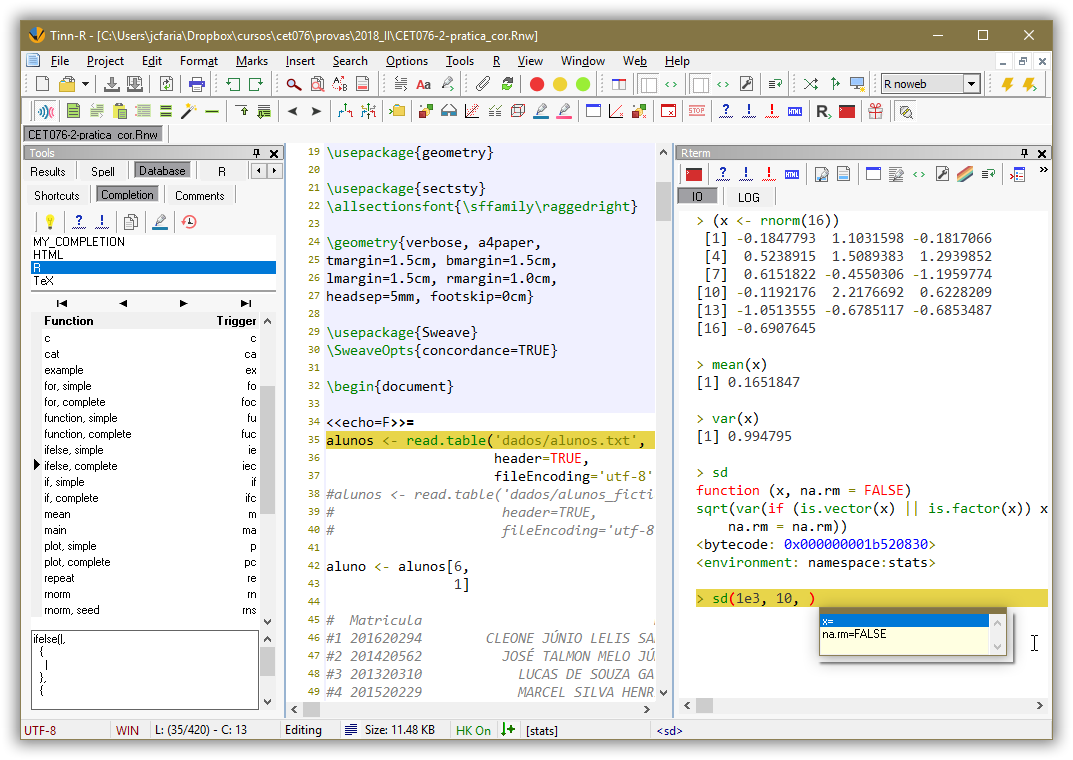
\includegraphics[width=\headwidth]{./res/general.png}
  \end{center}
  \caption{Tinn-R screenshot.}
  \label{fig:tinn-r_screenshot}
\end{figure}

\href{http://tinn.solarvoid.com}{Tinn} is a small ASCII file
editor primarily intended as a better replacement for the default Notepad 
running under the Windows OS. The name is the recursive acronym: 
\underline{T}inn \underline{i}s \underline{n}ot \underline{N}otepad.

\href{https://tinn-r.org/en/}{Tinn-R}
(Figure \ref{fig:tinn-r_screenshot})
is an extension of the original Tinn editor (ASCII and UNICODE), providing additional functionality
to control \href{http://cran.r-project.org}{R} running as Rgui
(in SDI mode) or Rterm and a whole lot of additional resources.

Tinn-R can also be thought of as feature-rich replacement of the basic 
script editor provided with Rgui. It provides syntax-highlighting, code 
submission as a whole or line-by-line, in addition to many other useful 
tools to ease the writing and debugging of \RR{} code.

Both Tinn and Tinn-R are distributed under the 
\href{http://www.gnu.org/copyleft/gpl.html}{GPL 2} license or above.


\newpage
\hypertarget{overview_whytinnr}{}
\section{Why Tinn-R?}
\index{overview!why Tinn-R?}

Do you:

\begin{itemize}
  \item like the open source initiative?
  \item need a simple but powerful GUI/Editor for the \RR{} environment?
  \item enjoy the ability to have syntax highlighting in your source code?
  \item need a tool that is simple to use but with the capabilities of a mighty editor?
  \item need a tool to work with plain text files?
  \item need a tool with simple commands for working with \LaTeX, Sweave and Txt2tags?
  %\item want to have access to the functionality of commercial and professional products but without having to pay for it?
  \item want to have access to the functionality of commercial and professional products?
\end{itemize}

\textit{\textbf{If you have answered YES to any of the questions above, then Tinn-R is a good option for you!}}


\hypertarget{overview_whatdoyouget}{}
\section{What do you get by using Tinn-R?}
\index{overview!what do you get?}

\begin{itemize}
  \item The ability to communicate with the \RR{} environment by sending
    instructions, controling its processing, and receiving results:
    \begin{itemize}
      \item Rterm.exe
      \item Rgui.exe. From Tinn-R version 8.02.01.01 onwards, Rgui must be launched from within Tinn-R so that it is properly
          identified at startup
    \end{itemize}
  \item Projects:
    \begin{itemize}
      \item Create project files to organize your work including 
        one level of sub-folders and automatic file name sorting
      \item Easy project management in graphical and text modes
    \end{itemize}
  \item Work with unlimited length files
  \item Work on multiple documents at the same time, choosing 
    between multiple-document interface (MDI) and tabbed 
    document interface (TDI)
  \item Single-document window splitting
  \item Support to macros (volatile):
    \begin{itemize}
      \item Record
      \item Playback commonly used sequences
    \end{itemize}
  \item Search and replace not restricted to your active file, but 
    also extendable to all open files, all project files, or any 
    folder
  \item View file differences with color highlighting
  \item Syntax highlighting, which can be set by file type
  \item Spell checking
  \item Multiple undo/redo
  \item Highlighted color syntax with print preview
  \item Ability to select:
    \begin{itemize}
      \item Normal
      \item Column
      \item Lines
    \end{itemize}
  \item Ability to bookmark:
    \begin{itemize}
      \item Line
      \item Block
    \end{itemize}
  \item Line numbers
  \item Special characters
  \item Sort multiple variable types:
    \begin{itemize}
      \item String
      \item Data
      \item Number
    \end{itemize}
  \item Count:
    \begin{itemize}
      \item Character
      \item Words
      \item Spaces
    \end{itemize}
  \item ASCII chart
  \item Export with highlight to clipboard RTF
  \item Matching bracket highlighting
  \item Conversion tools:
    \begin{itemize}
      \item Pandoc
      \item Deplate
      \item Txt2tags
    \end{itemize}
  \item \LaTeX ~support:
    \begin{itemize}
      \item Edition
      \item Compilation
      \item Inverse DVI search.
    \end{itemize}
\end{itemize}

We are constantly on the move!


\section{Do I have to pay for Tinn-R?}

The Tinn-R Team have been developing Tinn-R project under the GPL since june of 2003 (almost 15 years).
All this time it was distributed as free software. Currently, there are corporative
alternatives (paid or free as RStudio and RTVS) to lead with R environment. So, to cover the costs,
we are evaluating the possibility that it will be distributed as sharewere in the near future.

\section{What was the motivation to start and maintain the Tinn-R project?}

\begin{description}
  \item[Motivation to start Tinn-R:]
    We could not find a GUI/Editor for \RR{} running in the Windows OS that
    would give us all the ease of use and flexibility we wanted. So, we 
    started this project using an open source editor called 
    \href{http://tinn.solarvoid.com}{Tinn} as our initial
    platform.
  \item[Motivation to maintain Tinn-R:]
    The most difficult phase of the project was getting started: choosing
    the editor; all the preliminary performance and stability tests;
    understanding source structure; among many other struggles. Making
    it to run more and more smoothly and according to our daily needs was
    then a natural consequence. This is all to say that the open source
    movement has substantially changed our lives for better. We strongly
    believe in making software more widely available so that more people
    can benefit from it. We consider Tinn-R to be our small contribution
    to this fantastic open source initiative.
\end{description}


\section{What is the sentence that we, from the development team, most like to hear?}

Tinn-R made my life easier ... thanks for creating it.

% I wonder the below it is not necessary to the ebook! jcfaria
%\section{Which tools were used to create this user guide?}

%\begin{itemize}
%  \item Tinn-R was used to:
%    \begin{itemize}
%      \item Organize all source files under our project directory;
%      \item Edit the Txt2tags source files;
%      \item Manage the conversion and visualization of the final HTML code;
%    \end{itemize}
%  \item To manage external resources available within Tinn-R we used the following:
%    \begin{itemize}
%      \item Txt2tags, a python script to make the conversion from Txt2tags to HTML;
%      \item Python interpreter;
%      \item CSS to create the layout of the HTML content;
%    \end{itemize}
%  \item Pictures:
%    \begin{itemize}
%      \item \href{http://www.irfanview.com/}{IrfanView} was used
%        to select areas of the figures created using print screen function.
%    \end{itemize}
%\end{itemize}

%\begin{quotation}
%  That was all!
%\end{quotation}

%This user guide can be easily converted to the following formats: HTML, 
%XHTML, SGML, LaTeX, Lout, UNIX man page, Wikipedia, Google Code Wiki, 
%DokuWiki, MoinMoin, MagicPoint (mgp), and PageMaker. Just use the 
%Tinn-R GUI/Editor to do that.


\section{Acknowledgment}

We would like to thank those who have assisted us with the Tinn-R project, 
either by sending suggestions or by contributing to its development.


\section{Feedback, suggestions and bug reports}
\index{overview!bug reports}

Please submit feedback to 
\href{mailto:joseclaudio.faria@gmail.com}{Jos� Cl�udio Faria}.
If you submit a bug report, please provide as much detail as possible. This 
includes indicating the Tinn-R version, your operating system (Windows XP, 
Windows 7, etc) and language (English, French, Portuguese). If the bug is 
related to an interface with \RR{}, please also indicate which version of \RR{}
you are using, as well as whether you are running Rterm or Rgui. Ideally, 
please also add the content of the \textit{Tools/Results/Ini log} interface 
since this will help us address the issue more promptly.

\section{What tools were used to make this guide?}

It were used mainly:
\begin{enumerate}
   \item \href{https://tinn-r.org/en/}{Tinn-R}
    to edit, manager (as project) and submit to compilation the \LaTeX ~source files;
   \item \href{http://texstudio.sourceforge.net/}{\TeX studio}
    was also used in some parts where, to improve the productivity, it was necessary a more specialized \LaTeX ~editor;
   \item \href{http://www.vim.org/}{Vim}
    and 
    \href{https://github.com/LaTeX-Box-Team/LaTeX-Box}{\LaTeX ~Box plugin}
    when working under openSUSE (the actual preferred OS of the project leader);
   \item \href{http://www.ntwind.com/software/winsnap.html}{WinSnap}
    to get all images from the application;
   \item \href{http://www.faststone.org/}{FastStone Image Viewer}
    to browser and manager images;
   \item \href{http://www.r-project.org/}{R}
    as interpreter;
   \item \href{http://miktex.org/}{Mik\TeX}
    to compile the \LaTeX ~source files to final PDF format;
   \item \href{http://blog.kowalczyk.info/software/sumatrapdf/free-pdf-reader.html}{SumatraPDF} as PDF viewer.
\end{enumerate}
         % Tinn-R Overview

% DW: Experimental:
\renewcommand{\subsubsection} {\textsl{ }\\ }

% DW: Check \Rtables positioning
% workaround: \vspace{-0.5cm}

\hypertarget{basic}{}
\chapter{Basics}

This chapter provides the basics about the Tinn-R project.

\newpage

\hypertarget{basic_configuration}{}
\section{Configuration}
\index{configuration}

This section provides information on Tinn-R configuration and associated
applications.


\subsection{Uninstall Tinn-R}
\index{installation}

\begin{itemize}
  \item \textbf{ALWAYS UNISTALL ANY PRIOR VERSION OF Tinn-R BEFORE
      INSTALLING A NEW ONE!} Tinn-R has its own uninstall option.
  \item The folder where Tinn-R project stores the ini files will
    not be removed when unistalling it. Why? Because whenever you
    install a different version all your preferences will be
    preserved.
  \item You can check where these files are located by checking
    \textit{Help/Ini files (path information)}. If you prefer,
    you may delete these settings by removing the entire folder manually.
    \textbf{All your preferences will be lost forever if you don't
      have a backup file}.
\end{itemize}


\hypertarget{basic_configuration_installconfigure}{}
\subsection{Install and configure Tinn-R and R}


\subsubsection{R basic configuration:}\\

\begin{itemize}
  \item Starting from version 1.18.X.X, \texttt{Tinn-R requires
      Rgui.exe to run in SDI mode}. So, Tinn-R is not compatible neither
    with Rgui.exe in MDI mode (only SDI) nor with S-PLUS. The
    latest compatible version was the historic 1.17.2.4.
  \item Starting from version 2.0.0.0, \texttt{Tinn-R requires
      \RR{} to run either Rterm.exe or Rgui.exe (in SDI mode)}.
  \item Starting from version 8.02.01.01, Rgui.exe must be launched from within Tinn-R so that it is properly
          identified at startup.
  \item You have three basic options in order to switch Rgui.exe from
    MDI to SDI:
    \begin{enumerate}
      \item In Rgui.exe, select \texttt{Edit/GUI preferences...},
        set SDI and click on \texttt{Save}, then \texttt{OK}
        without changing the name of the proposed file. Then,
        click \texttt{OK} or \texttt{Cancel} in the
        \texttt{Rgui.exe Configuration Editor} (ignore any eventual
        messages), and restart Rgui.exe (changes will not be taken
        into account in the current session).
      \item Manually edit the file \texttt{Rconsole}:
        \begin{Scode}
          ## Style
          # This can be yes (for MDI) or no (for SDI).
          MDI = no
        \end{Scode}
      \item Create a shortcut to \RR{} on your desktop (or anywhere that is convenient),
        and type in the switch \texttt{--sdi} after the \texttt{...$\backslash$Rgui.exe}
        in the \texttt{Target} box. To do this, right click on your shortcut, select
        \texttt{Properties} and navigate to the \texttt{Shortcut} tab.
    \end{enumerate}
\end{itemize}


\subsubsection{If you have any version of Tinn-R ($>$= 3.0.1.0) installed:}\\

If your version is the same or above 3.0.1.0, Tinn-R does not require any special configuration.
That is, the program is ready to be used. One important thing to be done before using it:
set a \RR{} mirror as close as possible to where you work. For that, first click on \texttt{CTRL + F8}.
This opens the \texttt{Tools} window, then click on \texttt{R/Mirrors}.
Select the \RR{} mirror and push the button that shows an hourglass in the taskbar.
The chosen repository will be the new default for all actions dependent repository
(install packages, upgrade packages, etc).


\subsubsection{If you have any version of Tinn-R ($<$= 2.2.0.2) installed:}\\

\begin{enumerate}
  \item Uninstall previous versions of Tinn-R
  \item Edit the file Rprofile.site (folder \textit{etc} where
    \RR{} is installed) and comment (or remove) all prior configuration
    scripts RELATED TO TINN-R
  \item Start \RR{}
  \item Install the following packages:
    \begin{enumerate}
      \item \href{http://cran.r-project.org/web/packages/TinnR/index.html}{TinnR}
      \item \href{http://cran.r-project.org/web/packages/svSocket/index.html}{svSocket}
      \item \href{http://cran.r-project.org/web/packages/formatR/index.html}{formatR}
    \end{enumerate}
  \item Close \RR{}
  \item Install the new version of Tinn-R
  \item Start Tinn-R
  \item From the Tinn-R main menu, choose the option
    \texttt{R/Configure/Permanent (Rprofile.site)}. It will write the
    following text to the file Rprofile.site:
    {\footnotesize
      {\color {darkred}
        \begin{verbatim}
          ##===============================================================
          ## Tinn-R: necessary packages and functions
          ## Tinn-R: >= 2.4.1.1 with TinnR package >= 1.0.3
          ##===============================================================
          ## Set the URL of the preferred repository, below some examples:
          options(repos='http://cran.at.r-project.org/')      # Austria/Wien
          #options(repos='http://cran-r.c3sl.ufpr.br/')       # Brazil/PR
          #options(repos='http://cran.fiocruz.br/')           # Brazil/RJ
          #options(repos='http://www.vps.fmvz.usp.br/CRAN/')  # Brazil/SP
          #options(repos='http://brieger.esalq.usp.br/CRAN/') # Brazil/SP

          library(utils)

          ## Check necessary packages
          necessary <- c('TinnR',
                         'svSocket',
                         'formatR')

          installed <- necessary %in% installed.packages()[, 'Package']
          if (length(necessary[!installed]) >=1)
          install.packages(necessary[!installed])

          ## Load packages
          library(TinnR)
          library(svSocket)

          ## Uncomment the two lines below if you want Tinn-R to always start R at start-up
          ## (Observation: check the path of Tinn-R.exe)
          #options(IDE='C:/Tinn-R/bin/Tinn-R.exe')
          #trStartIDE()

          ## Option
          options(use.DDE=T)

          ## Start DDE
          trDDEInstall()

          ## Short paths
          .trPaths <- paste(paste(Sys.getenv('APPDATA'),
                                  '\\Tinn-R\\tmp\\',
                                  sep=''),
                      c('',
                        'search.txt',
                        'objects.txt',
                        'file.r',
                        'selection.r',
                        'block.r',
                        'lines.r',
                        'reformat-input.r',
                        'reformat-output.r'),
                      sep='')
        \end{verbatim}
      } % color
    } % footnotesize
  \item Start Rgui.exe or Rterm.exe from within Tinn-R
  \item Read the content from the links below:
    \begin{itemize}
      \item \textit{\href{\#basic\_card}{Card}}: to know
        the shortcuts related with \RR{} and all others
      \item \textit{\href{\#whatisnew}{What is new}}:
        to know the news.
    \end{itemize}
\end{enumerate}


Information about how to customize the \texttt{Rprofile.site} file can be obtained from
\href{http://stat.ethz.ch/R-manual/R-patched/library/base/html/Startup.html}{Initialization at Start of an R Session}
and an example of this file from \href{http://sourceforge.net/p/tinn-r/news/?source=navbar}{SourceForge}.


\subsubsection{If you have any version of Tinn-R ($>$= 2.2.0.2) installed and configured:}\\

\begin{enumerate}
  \item Uninstall the prior version of Tinn-R 2.X.X.X
  \item Install the new version of Tinn-R
  \item Run it.
\end{enumerate}


\subsubsection{If you want to install any old version of Tinn-R ($<$= 2.0.0.0"):}\\

\begin{itemize}
  \item \textbf{Downgrading}: \texttt{rename (or delete) the folder
      where Tinn-R stores the ini files}. The uninstall is necessary
    since Tinn-R does not downgrade automatically. If you encounter
    any problems while downgrading, check the ini folder and respective
    files.
  \item Download and install Tinn-R.
  \item Install the \texttt{SciViews} bundle, then type
    \texttt{guiDDEInstall()} in \RR{} and \texttt{that's all}!

    \begin{footnotesize}
      \begin{verbatim}
        > install.packages('SciViews', dep=T)
        > guiDDEInstall()
      \end{verbatim}
    \end{footnotesize}

  \item Perhaps the best way to get \RR{} to communicate with
    Tinn-R from the time it is started is to add the
    following commands to \texttt{../etc/Rprofile.site}
    in the \RR{} install directory:

    \begin{Scode}
      #===============================================================
      # Tinn-R: necessary packages and functions
      #===============================================================
      library(utils)
      necessary = c('svIDE', 'svIO', 'svSocket', 'R2HTML')
      installed = necessary %in% installed.packages()[, 'Package']
      if (length(necessary[!installed]) >=1)
      install.packages(necessary[!installed], dep = T)

      library(svIDE)
      library(svIO)
      library(svSocket)
      library(R2HTML)
      guiDDEInstall()
    \end{Scode}

  \item If you chose the latter option \texttt{.../etc/Rprofile.site},
    a nice additional functionality is provided by adding the two
    lines below \texttt{BEFORE} the \texttt{library(svIDE)} command:

    \begin{Scode}
      options(IDE = 'C:/Tinn-R/bin/Tinn-R.exe')
      options(use.DDE = T)
    \end{Scode}

    The first line tells \RR{} that you want to use Tinn-R as your IDE (Integrated
    Development Environment).  To make this happen, you should change the path
    that leads to where \texttt{Tinn-R.exe} is installed if it happens to be
    different from the default configuration. The second line indicates that
    you want to start the DDE server automatically.

    By doing this, Tinn-R will start automatically once you invoke \RR{}.
\end{itemize}


\subsection{Rgui.exe}
\index{Rgui}

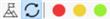
\includegraphics[scale=0.50]{./res/focus.png}

\begin{itemize}
  \item Tinn-R has an icon within the \textit{Options toolbar}
    containing the hint \texttt{Options: return focus to editor
      after send/control Rgui.exe} which enables the user to configure
    the focus control. When \texttt{checked}:
    \begin{itemize}
      \item If the editor has the focus: it will \texttt{go back}
        to the editor after any \textit{send to} or \textit{R control}
        action;
      \item Otherwise, the focus will be set to the Rgui.exe interface.
    \end{itemize}
\end{itemize}


\subsection{Rterm.exe}
\index{Rterm}

\begin{itemize}
  \item The above-mentioned icon will be disabled with Term interface.
    The following will then happen:
    \begin{itemize}
      \item If the focus is placed on the editor it will \texttt{go back}
        to the editor after any \textit{send to} or \textit{R control} action;
      \item If the focus is placed on the Term (\textit{IO} or \textit{LOG}),
        it will be \texttt{maintened} in this interface (\textit{IO});
      \item Situations above are also the case when working with two monitors.
    \end{itemize}
\end{itemize}


\newpage
\subsection{Term interface and debug package}
\index{debugging}

\begin{itemize}
  \item Several changes were made to the debug package (1.0.2) regarding
    the messaging system (\textit{stdout} and \textit{stderr}). The
    default option is no longer compatible with Term interface
    implementation.
  \item The best way to make it compatible again is to add the option
    below to the Rprofile.site file:

    \begin{footnotesize}
      \begin{verbatim}
        options(debug.catfile = 'stdout')
      \end{verbatim}
    \end{footnotesize}

   \item This option is automatically sent to the \RR{} interpreter from version 3.0.3.0 of Tinn-R project.
\end{itemize}


\hypertarget{configuration_spellerinstalation}{}
\subsection{Speller installation}
\index{speller}

\begin{itemize}
  \item To install this resource:
    \begin{enumerate}
      \item Close Tinn-R (if it is running);
      \item Download the
        \href{http://www.luziusschneider.com/Speller/English/index.htm}{dictionaries}
        you would like to add to Tinn-R;
      \item Install the file (for example ISpEnFrGe.exe);
    \end{enumerate}
  \item Upon start, Tinn-R will recognize all installed dictionaries.
    You should choose one as your default.
  \item Before installing new dictionaries, it is strongly
    recommended that you close Tinn-R.
  \item Another useful tool is the \texttt{UserDicEditor} which
    enables the editing of dictionaries.
\end{itemize}


\subsection{Inverse DVI search}
\index{inverse DVI search}
\index{search!inverse DVI }
\index{DVI!inverse search}

\begin{itemize}
  \item Tinn-R is able to perform \texttt{inverse DVI search}. To get this
    function to work, include in your DVI previewer the path of the
    binary executable file for Tinn-R along with the parameters for
    file and line.  For example, using YAP under Miktex, the configuration
    would be (assuming a default path for Tinn-R):
    \index{Miktex}

    \begin{footnotesize}
      \begin{verbatim}
        C:\Tinn-R\bin\Tinn-R.exe "%f;%l"
        
        Note:
        %f: file
        %l: line
      \end{verbatim}
    \end{footnotesize}

    \begin{itemize}
      \item Please make sure that there is no space between the
        parameters \%f(related to file) and \%l(related to line);\\\\
        \includegraphics[scale=0.50]{./res/yap_01.png}~~
        \includegraphics[scale=0.50]{./res/yap_02.png}\\
      \item It is necessary to add the parameter for \TeX~Live or Mik\TeX~compilation
        within Tinn-R (\textit{Options/Application/Processing/Latex/DVI}):
        latex -c-style-errors \texttt{--src-specials};

        \begin{footnotesize}
          \begin{verbatim}
            latex -c-style-errors --src-specials
            and
            bibtex --src-specials
          \end{verbatim}
        \end{footnotesize}

        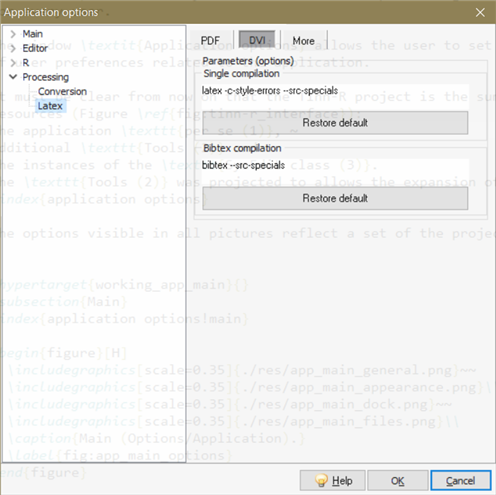
\includegraphics[scale=0.50]{./res/app_processing_latex_dvi.png}\\
    \end{itemize}
\end{itemize}


\subsection{Inverse PDF search}
\index{inverse PDF search}
\index{search!inverse PDF}
\index{PDF!inverse search}

\begin{itemize}
  \item Tinn-R is able to perform \texttt{inverse PDF search}. To get this
    function to work, include in your PDF previewer (we recomend Sumatra) the path of the
    binary executable file for Tinn-R along with the parameters for
    file and line.  For example, using Sumatra, the configuration
    would be (assuming a default path for Tinn-R):
    \index{Sumatra}

    \begin{footnotesize}
      \begin{verbatim}
        C:\Tinn-R\bin\Tinn-R.exe "%f;%l"
        
        Note:
        %f: file
        %l: line
      \end{verbatim}
    \end{footnotesize}

    \begin{itemize}
      \item Please make sure that there is no space between the
        parameters \%f(related to file) and \%l(related to line);\\\\
        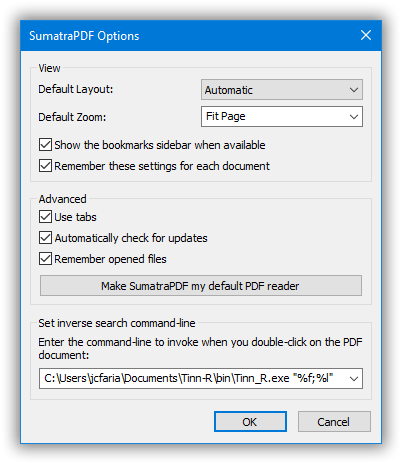
\includegraphics[scale=0.80]{./res/sumatra.png}\\
      \item It is necessary to add the parameter for Miktex compilation
        within Tinn-R (\textit{Options/Application/Processing/Latex/PDF}):
        pdflatex -c-style-errors \texttt{ --synctex=1};
      \item Tinn-R can do all of this automatically by setting the
        option \textit{Restore default}:

        \begin{footnotesize}
          \begin{verbatim}
            pdflatex -c-style-errors --synctex=1
            and
            bibtex
          \end{verbatim}
        \end{footnotesize}

        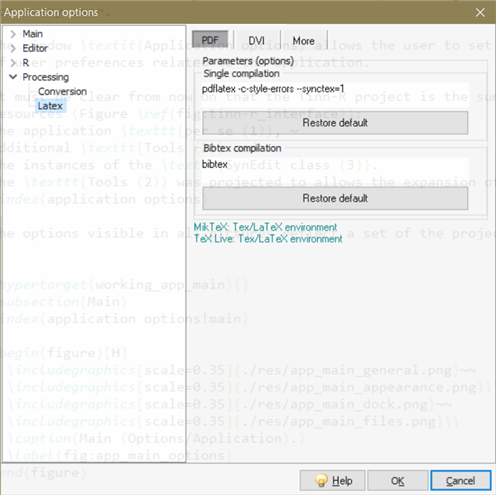
\includegraphics[scale=0.60]{./res/app_processing_latex_pdf.png}\\
    \end{itemize}
\end{itemize}


\subsection{Ruby and Deplate}
\index{Ruby}
\index{Deplate}

\begin{itemize}
  \item \href{http://deplate.sourceforge.net/}{Deplate}
    \href{http://deplate.sourceforge.net/deplate.html}{(user guide here)}
    is a remote
    \href{http://www.ruby-lang.org/en/}{Ruby} based tool for
    converting documents written in wiki-like markup to \LaTeX, HTML, HTML slides,
    or DocBook format. Deplate supports page templates, embedded \LaTeX ~code,
    footnotes, citations, bibliographies, automatic generation of indices, tables
    of contents, among others. Deplate can also be used to create Web pages and,
    via \LaTeX ~or DocBook, high-quality printouts.

  \item Tinn-R works with the Ruby interpreter for Windows (ruby.exe) and Ruby
    scripts to generate file conversation within deplate.

  \item To install and configure these resources follow these steps:
    \begin{enumerate}
      \item Download and unzip the
        \href{http://www.ruby-lang.org/en/}{Ruby}
        interpreter anywhere in your computer;
      \item Download and unzip
        \href{http://deplate.sourceforge.net/Download.php}{Deplate}
        anywhere in your computer;
      \item Within Tinn-R, go to \texttt{Options/Application/Processing/Conversion/Deplate}
        and add information on parameters (\texttt{-f} is the default),
        the interpreter path (\texttt{ruby.exe}), and the converter
        (\texttt{deplate.rb ruby script});\\

        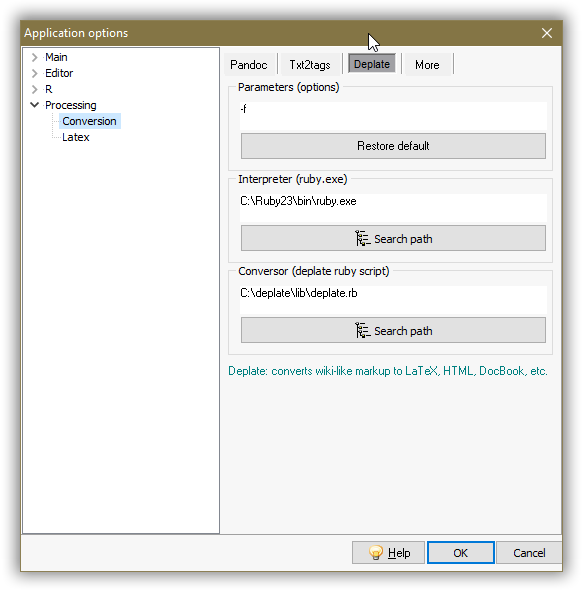
\includegraphics[scale=0.50]{./res/app_processing_conversion_deplate.png}\\
    \end{enumerate}
\end{itemize}

The conversion options using \texttt{Deplate} depends of the file extension.
Are recognized: \texttt{.dp, .dpt, .dplt, .deplate and .txt}.

We recently observed a problem when converting files with file names with an
underscore. For example \texttt{deplate\_intro.dplt}. In these cases the file
conversion is completed, but Tinn-R won't open the file since it can't find it.
This pattern is caused by Deplate (a ruby script) generating a file named
\texttt{deplate\_\_intro.html}. \textit{Observe that this file name contains a
double underscore}. In sum, for the time being, avoid underscores in file
names when you intend to convert them later through Deplate.


\subsection{Pandoc}
\index{Pandoc}

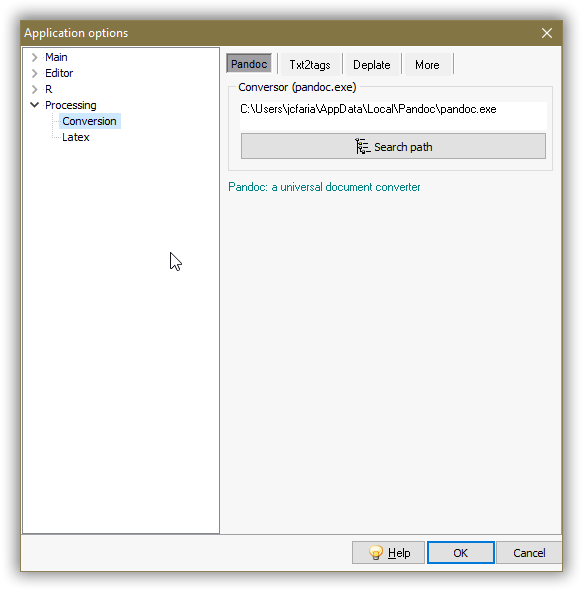
\includegraphics[scale=0.50]{./res/app_processing_conversion_pandoc.png}

\begin{itemize}
\item If you need to convert files from one markup format into another, \href{http://johnmacfarlane.net/pandoc/index.html}{Pandoc} is your swiss-army knife.
\item To install and configure Pandoc resources, just follow these steps:
 \begin{enumerate}
 \item \href{http://code.google.com/p/pandoc/downloads/list}{Download} and install the converter Pandoc anywhere in your computer;
 \item Within Tinn-R, go to \texttt{Options/Application/Processing/Conversion/Pandoc} and add information on path (\texttt{pandoc.exe}).

 \end{enumerate}
\item Pandoc can \href{http://johnmacfarlane.net/pandoc/README.html}{convert} documents:
\end{itemize}

\begin{footnotesize}\begin{tabularx}{130pt}{lX} \\
\hline
\textbf{From} \\
\hline
  DocBook \\
  HTML \\
  JSON version of native AST \\
  \LaTeX \\
  markdown \\
  native Haskell \\
  reStructuredText \\
  textile \\
\hline
\end{tabularx}\end{footnotesize}

\begin{footnotesize}\begin{tabularx}{\textwidth}{>{\hsize=0.4\hsize}X>{\hsize=0.7\hsize}X} \\
    \hline
    \textbf{To} & \textbf{Subset(s)} \\
    \hline
    Documentation formats & DocBook, GNU TexInfo, Groff man pages \\
    Ebooks & EPUB \\
    HTML formats & XHTML, HTML5, and HTML slide shows using Slidy, Slideous, S5, or DZSlides \\
    Lightweight markup formats & Markdown, reStructuredText, AsciiDoc, MediaWiki markup, Emacs Org-Mode, Textile \\
    PDF via \LaTeX \\
    TeX formats & \LaTeX, ConTeXt, \LaTeX Beamer slides \\
    Word processor formats & Microsoft Word docx, OpenOffice/LibreOffice ODT, OpenDocument XML \\
    \hline
  \end{tabularx}\end{footnotesize}


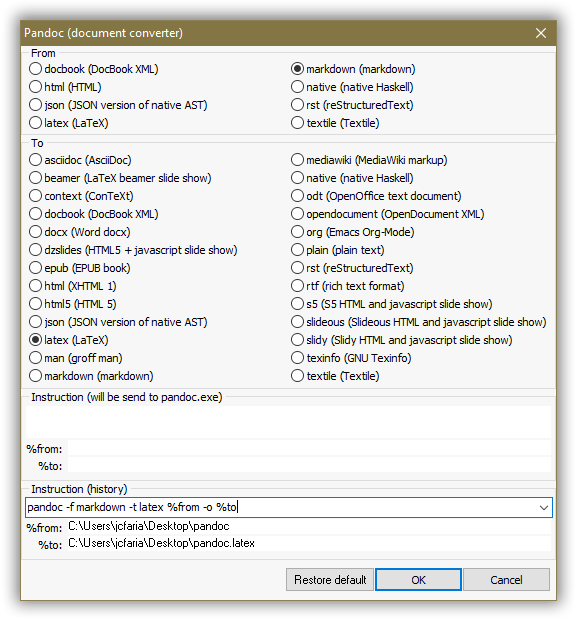
\includegraphics[scale=0.50]{./res/pandoc.png}

\subsection{Python and Txt2tags}
\index{Python}
\index{Txt2tags}

\begin{itemize}
  \item \href{http://txt2tags.sourceforge.net}{Txt2tags}
    \href{http://txt2tags.sourceforge.net/userguide}{(user guide here)}
    converts a text file with \texttt{minimal and human readable markup} to:
    HTML, XHTML, SGML, \LaTeX, Lout, UNIX man page, Wikipedia, Google Code Wiki,
    DokuWiki, MoinMoin, MagicPoint (mgp), and PageMaker. It is simple and fast,
    featuring automatic TOC, macros, filters, include, tools, GUI, CLI,
    Web interfaces, translations, and extensive documentation.

  \item Tinn-R works with the Phyton interpreter for Windows (python.exe), using
    Python scripts to make the conversion (txt2tags).

  \item To install and configure Python resources, just follow these steps:
    \begin{enumerate}
      \item Download and install the
        \href{http://www.python.org/download/}{Python}
        interpreter anywhere in your computer;
      \item Download and unzip
        \href{http://txt2tags.sourceforge.net/}{Txt2tags}
        anywhere in your computer;
      \item Within Tinn-R, go to \texttt{Options/Application/Processing/Txt2tags}
        and add information on parameters (\texttt{-t} is the default),
        interpreter path (\texttt{python.exe}) and the
        converter (\texttt{txt2tags python script});\\

        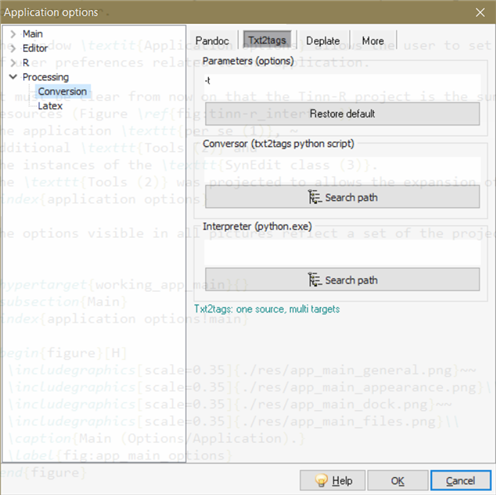
\includegraphics[scale=0.50]{./res/app_processing_conversion_txt2tags.png}\\
    \end{enumerate}
\end{itemize}

The conversion options using \texttt{Txt2tags} depends of the file extension.
Are recognized: \texttt{.t2, .t2t, .txt2tags. and .txt}.

\newpage

\hypertarget{basic_card}{}
\section{Keyboard shortcuts (default)}
\index{keyboard shortcuts}

This section provides information about keyboard shortcuts.

\hypertarget{basic_card_mostused}{}
\subsubsection{R interface:}
\index{keyboard shortcuts!R interface}

% =============================================================================
\vspace{-0.5cm}
\begin{Rtables}[caption={[R interface keyboard shortcuts]
    R interface keyboard shortcuts},
  label=hotkey:rinterface]
  ALT  + DOWN            : R history: down (IO)
  ALT  + E               : R echo (on/off)
  ALT  + L               : Clear (LOG)
  ALT  + LEFT            : Editor: set focus
  ALT  + PGDN            : LOG: set focus
  ALT  + RIGHT           : IO: set focus
  ALT  + UP              : R history: up (IO)
  ALT  + CTRL + SPACE    : R history completion window (IO)
  CTRL + -               : Insert <-
  CTRL + +               : Insert ->
  CTRL + ENTER           : Send any line or sel. (single line only) (IO)
  CTRL + F1              : Example on selected word*
  CTRL + F2              : Open example on selected word*
  CTRL + L               : Clear (IO)
  CTRL + SPACE           : Tip after '(' and completion after '$'
  CTRL + TAB             : Change seq. IO and LOG to the right**
  CTRL + TIL             : Send current file to Sweave
  SHIFT + CTRL + TAB     : Change seq. IO and LOG to the left**
  F1                     : Help on selected word*
  SHIFT + CTRL + B       : Clear (IO and LOG)
  SHIFT + CTRL + F1      : R help (HTML)*
  *  (requires an R session)
  ** (requires focus)
\end{Rtables}
% =============================================================================


\subsubsection{Visualization:}
\index{keyboard shortcuts!vizualization}

% =============================================================================
\vspace{-0.5cm}
\begin{Rtables}[caption={[Visualization keyboard shortcuts]
    Visualization keyboard shortcuts},
  label=hotkey:visualization]
  CTRL  + F8              : Tools: visible (show/hide)
  CTRL  + F9              : R interface: visible (show/hide)
  CTRL  + F10             : R interface: minimize
  CTRL  + F11             : R interface: optimize
  CTRL  + F12             : R interface: maximize
  CTRL  + ALT  + G        : Gutter (show/hide)
  CTRL  + ALT  + L        : Line number (show/hide)
  CTRL  + ALT  + K        : Special characters (show/hide)
  CTRL  + ALT  + V        : Tool bars: all (show/hide)
  CTRL  + TAB             : Change seq. the active page
                            (Editor, RTerm an Help) to the right*
  CTRL  + SHIFT + TAB     : Change seq. the active page
                            (Editor, RTerm an Help) to the left*
  SHIFT + CTRL + +        : Increase font size**
  SHIFT + CTRL + -        : Decrease font size**
  *  (requires more than one)
  ** (text within the main interface)
\end{Rtables}
% =============================================================================


\newpage
\subsubsection{Navigation:}
\index{keyboard shortcuts!navigation}

% =============================================================================
\vspace{-0.5cm}
\begin{Rtables}[caption={[Navigation keyboard shortcuts]
    Navigation keyboard shortcuts},
  label=hotkey:navigation]
  CTRL  + END             : End of a doc
  CTRL  + HOME            : Beginning of a doc
  END                     : End of a line
  HOME                    : Beginning of a line
\end{Rtables}
% =============================================================================

\subsubsection{Search/Replace and Go:}
\index{keyboard shortcuts!search/replace and go}

% =============================================================================
\vspace{-0.5cm}
\begin{Rtables}[caption={[Search/Replace and go keyboard shortcuts]
    Search/Replace and go keyboard shortcuts},
  label=hotkey:search]
  CTRL  + F               : Find
  F3                      : Find again
  SHIFT + CTRL + F        : Search in files
  CTRL  + R               : Replace
  CTRL  + G               : Go to line
\end{Rtables}
% =============================================================================


\subsubsection{Function Keys:}
\index{keyboard shortcuts!function keys}

% =============================================================================
\vspace{-0.5cm}
\begin{Rtables}[caption={[Function keys]
    Function keys},
  label=hotkey:function]
  F1                      : Help on selected word*
  F2                      : List the structure of selected object*
  F3                      : Find again
  F7                      : Macro record
  F8                      : Macro play
  F9                      : Clear the R console*
  F10                     : Close all graphic devices*
  F11                     : Remove all objects*
  F12                     : Clear all*
  * (requires an R session)
\end{Rtables}
% =============================================================================


\newpage
\subsubsection{Edition:}
\index{keyboard shortcuts!edition}

% =============================================================================
\vspace{-0.5cm}
\begin{Rtables}[caption={[Edition keyboard shortcuts]
    Edition keyboard shortcuts},
  label=hotkey:editions]
  ALT   + C               : Block comment
  ALT   + N               : Block uncomment (first ocurrence)
  ALT   + Z               : Block uncomment (all ocurrence)
  CTRL  + (               : Insert (or replace) (|)
  CTRL  + )               : Insert (or replace) ()
  CTRL  + A               : Select all
  CTRL  + C               : Copy
  CTRL  + END             : End doc
  CTRL  + HOME            : Beginning of a doc
  CTRL  + I               : Block indent
  CTRL  + T               : Delete word
  CTRL  + U               : Block unindent
  CTRL  + V               : Paste
  CTRL  + X               : Cut
  CTRL  + Y               : Delete line
  CTRL  + Z               : Undo
  END                     : End of a line
  HOME                    : Beginning of a line
  SHIFT + CTRL + Z        : Redo
\end{Rtables}
% =============================================================================


\subsubsection{Marks and Go to Marks:}
\index{keyboard shortcuts!marks}

% =============================================================================
\vspace{-0.5cm}
\begin{Rtables}[caption={[Marks and go to marks keyboard shortcuts]
    Marks and go to marks keyboard shortcuts},
  label=hotkey:marks]
  CTRL  + NUMBER[0..9]        : Go to mark (no numeric keypad)
  SHIFT + CTRL + NUMBER[0..9] : Mark (no numeric keypad)
\end{Rtables}
% =============================================================================


\subsubsection{Project:}
\index{keyboard shortcuts!project}

% =============================================================================
\vspace{-0.5cm}
\begin{Rtables}[caption={[Project keyboard shortcuts]
    Project keyboard shortcuts},
  label=hotkey:project]
  CTRL  + INS             : Add current file to selected group
  SHIFT + CTRL + INS      : Add file(s) to selected group (with dialog)
  DEL                     : Delete selected group or file
\end{Rtables}
% =============================================================================


\subsubsection{R Script Edition:}
\index{keyboard shortcuts!R script edition}

% =============================================================================
\vspace{-0.5cm}
\begin{Rtables}[caption={[R script edition keyboard shortcuts]
    R script edition keyboard shortcuts},
  label=hotkey:rscript]
  CTRL + -                : Insert <-
  CTRL + -                : Insert <-  (numeric keypad)*
  CTRL + +                : Insert ->
  CTRL + +                : Insert ->  (numeric keypad)*
  CTRL + *                : Insert tip (numeric keypad)*
  CTRL + ENTER            : Send current line to R and insert a line break
  * (not configurable by user)
\end{Rtables}
% =============================================================================


\newpage
\subsubsection{Selection:}
\index{keyboard shortcuts!selection}

% =============================================================================
\vspace{-0.5cm}
\begin{Rtables}[caption={[Selection keyboard shortcuts]
    Selection keyboard shortcuts},
  label=hotkey:selection]
  CTRL  + ALT  + S        : Mark block
  CTRL  + ALT  + Z        : Unmark block
  CTRL  + ALT  + X        : Unmark all
  SHIFT + CTRL + C        : Selection: set to column mode
  SHIFT + CTRL + L        : Selection: set to line mode
  SHIFT + CTRL + N        : Selection: set to normal mode
\end{Rtables}
% =============================================================================


\subsubsection{Compilation:}
\index{keyboard shortcuts!compilation}

% =============================================================================
\vspace{-0.5cm}
\begin{Rtables}[caption={[Compilation keyboard shortcuts]
    Compilation keyboard shortcuts},
  label=hotkey:compilation]
  CTRL  + ALT  + D       : Compilation: LaTeX to DVI (single)
  CTRL  + ALT  + P       : Compilation: LaTeX to DVI (single)
  SHIFT + CTRL + ALT + D : Compilation: LaTeX to DVI (bibtex)
  SHIFT + CTRL + ALT + P : Compilation: LaTeX to PDF (bibtex)
  CTRL  + ALT  + I       : Compilation: Make index (makeindex)
\end{Rtables}
% =============================================================================


\subsubsection{Conversion and Visualization:}
\index{keyboard shortcuts!conversion}

% =============================================================================
\vspace{-0.5cm}
\begin{Rtables}[caption={[Conversion and visualization keyboard shortcuts]
    Conversion and visualization keyboard shortcuts},
  label=hotkey:conversion]
  SHIFT + CTRL + P       : Conversion: Pandoc*
  SHIFT + CTRL + O       : Open current HTML files**
  SHIFT + CTRL + U       : Open current file (generic)
  *  (a universal document converter)
  ** (with system default browser)
\end{Rtables}
% =============================================================================


\newpage
\hypertarget{basic_card_mainmenu}{}
\subsection{Main menu (systematically)}
\index{keyboard shortcuts!main menu}

% =============================================================================
\vspace{-0.5cm}
\begin{Rtables}[caption={[Main menu keyboard shortcuts]
    Main Menu keyboard shortcuts},
  label=menu:main]
  ALT + F                 : File
  ALT + P                 : Project
  ALT + E                 : Edit
  ALT + A                 : Format
  ALT + M                 : Marks
  ALT + I                 : Insert
  ALT + S                 : Search
  ALT + O                 : Options
  ALT + T                 : Tools
  ALT + R                 : R
  ALT + V                 : View
  ALT + D                 : Window
  ALT + B                 : Web
  ALT + H                 : Help
\end{Rtables}
% =============================================================================


\subsubsection{File:}
\index{keyboard shortcuts!file menu}

% =============================================================================
\vspace{-0.5cm}
\begin{Rtables}[caption={[File menu keyboard shortcuts]
    File menu keyboard shortcuts},
  label=menu:file]
  CTRL  + N               : New file
  CTRL  + O               : Open file
  CTRL  + P               : Print
  CTRL  + S               : Save file
  CTRL  + W               : Close file
  SHIFT + CTRL + R        : Reload file
  SHIFT + CTRL + S        : Save file as
  SHIFT + CTRL + W        : Close all files
\end{Rtables}
% =============================================================================


\subsubsection{Project:}
\index{keyboard shortcuts!project}

% =============================================================================
\vspace{-0.5cm}
\begin{Rtables}[caption={[Project menu keyboard shortcuts]
    Project keyboard shortcuts},
  label=menu:project]
  CTRL  + INS             : Add current file to selected group
  SHIFT + CTRL + INS      : Add file(s) to selected group (with dialog)
\end{Rtables}
% =============================================================================


\subsubsection{Edit:}
\index{keyboard shortcuts!edit}

% =============================================================================
\vspace{-0.5cm}
\begin{Rtables}[caption={[Edit menu keyboard shortcuts]
    Edit menu keyboard shortcuts},
  label=menu:edit]
  CTRL + Z                : Undo
  CTRL + SHIFT + Z        : Redo
  CTRL + C                : Copy
  CTRL + X                : Cut
  CTRL + V                : Paste
  CTRL + A                : Copy all
  ALT  + C                : Block/line comment
  ALT  + N                : Block/line uncomment first occurrence
  ALT  + Z                : Block/line uncomment all occurrences
\end{Rtables}
% =============================================================================


\newpage
\subsubsection{Format:}
\index{keyboard shortcuts!format}

% =============================================================================
\vspace{-0.5cm}
\begin{Rtables}[caption={[Format menu keyboard shortcuts]
    Format menu keyboard shortcuts},
  label=menu:format]
  CTRL + F5               : Reformat R (file or selection)
  CTRL + I                : Block indent
  CTRL + U                : Block unindent
\end{Rtables}
% =============================================================================


\subsubsection{Marks:}
\index{keyboard shortcuts!marks}

% =============================================================================
\vspace{-0.5cm}
\begin{Rtables}[caption={[Marks menu keyboard shortcuts]
    Marks menu keyboard shortcuts},
  label=menu:marks]
  CTRL  + NUMBER[0..9]        : Go to mark (no numeric keypad)
  SHIFT + CTRL + NUMBER[0..9] : Mark (no numeric keypad)
  CTRL  + ALT  + S            : Mark block
  CTRL  + ALT  + Z            : Unmark block
  CTRL  + ALT  + X            : Unmark all
\end{Rtables}
% =============================================================================


\subsubsection{Insert:}
\index{keyboard shortcuts!insert}

% =============================================================================
\vspace{-0.5cm}
\begin{Rtables}[caption={[Insert menu keyboard shortcuts]
    Insert menu keyboard shortcuts},
  label=menu:insert]
  CTRL + -               : Insert <-
  CTRL + +               : Insert ->
  CTRL + J               : Completion
  SHIFT + CTRL + I       : Insert dimensional element (LaTeX)
\end{Rtables}
% =============================================================================


\subsubsection{Search:}
\index{keyboard shortcuts!search}

% =============================================================================
\vspace{-0.5cm}
\begin{Rtables}[caption={[Search menu keyboard shortcuts]
    Search menu keyboard shortcuts},
  label=menu:search]
  CTRL + F                : Search text
  CTRL + G                : Go to
  CTRL + R                : Replace text
  F3                      : Search again
\end{Rtables}
% =============================================================================


\subsubsection{Options:}
\index{keyboard shortcuts!options}

% =============================================================================
\vspace{-0.5cm}
\begin{Rtables}[caption={[Options menu keyboard shortcuts]
    Options menu keyboard shortcuts},
  label=menu:options]
  CTRL  + ALT  + M        : Shortcuts/Keystrokes/hotkeys (map)
  ALT   + E               : R echo (on/off)
  CTRL  + ALT  + C        : Auto completion \verb{( [ { ' "}
  CTRL  + ALT  + N        : Enable notification
  CTRL  + ALT  + U        : Update silently
  SHIFT + CTRL + N        : Selection: set to normal mode
  SHIFT + CTRL + C        : Selection: set to column mode
  SHIFT + CTRL + L        : Selection: set to line mode
\end{Rtables}
% =============================================================================


\newpage
\subsubsection{Tools:}
\index{keyboard shortcuts!tools}

% =============================================================================
\vspace{-0.5cm}
\begin{Rtables}[caption={[Tools menu keyboard shortcuts]
    ToolsMenu keyboard shortcuts},
  label=menu:tools]
  SHIFT + CTRL + Down     : Sort strings
  SHIFT + CTRL + P        : Conversion: Pandoc*
  SHIFT + CTRL + O        : Open current HTML files**
  SHIFT + CTRL + U        : Open current file (generic)
  CTRL  + ALT  + D        : Compilation: LaTeX to DVI (single)
  CTRL  + ALT  + P        : Compilation: LaTeX to DVI (single)
  SHIFT + CTRL + ALT + D  : Compilation: LaTeX to DVI (bibtex)
  SHIFT + CTRL + ALT + P  : Compilation: LaTeX to PDF (bibtex)
  CTRL  + ALT  + I        : Compilation: Make index (makeindex)
  CTRL  + B               : Match bracket
  F7                      : Macro/Record
  F8                      : Macro/Play
  *  (a universal document converter)
  ** (with system default browser)
\end{Rtables}
% =============================================================================


\subsubsection{R:}
\index{keyboard shortcuts!R menu}

% =============================================================================
\vspace{-0.5cm}
\begin{Rtables}[caption={[R menu keyboard shortcuts]
    R menu keyboard shortcuts},
  label=menu:r]
  ALT  + L               : Clear (LOG)
  ALT  + LEFT            : Editor: set focus
  ALT  + PGDN            : LOG: set focus
  ALT  + RIGHT           : IO: set focus
  CTRL + F10             : R interface: minimize
  CTRL + F11             : R interface: optimize
  CTRL + F12             : R interface: maximize
  CTRL + F9              : R interface: visible (show/hide)
  CTRL + L               : Clear (IO)
  SHIFT + CTRL + B       : Clear (IO and LOG)
\end{Rtables}
% =============================================================================


\newpage
\subsubsection{View:}
\index{keyboard shortcuts!view}

% =============================================================================
\vspace{-0.5cm}
\begin{Rtables}[caption={[View menu keyboard shortcuts]
    View menu keyboard shortcuts},
  label=menu:view]
  ALT  + LEFT             : Editor: set focus
  ALT  + PGDN             : LOG: set focus
  ALT  + RIGHT            : IO: set focus
  ALT  + W                : Editor: line wrap (show/hide)
  CTRL + ALT + K          : Special characters (show/hide)
  CTRL + ALT + L          : Line number (show/hide)
  CTRL + ALT + V          : Tool bars: all (show/hide)
  CTRL + F10              : R interface: minimize
  CTRL + F11              : R interface: optimize
  CTRL + F12              : R interface: maximize
  CTRL + F8               : Tools: visible (show/hide)
  CTRL + F9               : R interface: visible (show/hide)
\end{Rtables}
% =============================================================================


\hypertarget{basic_card_calltip}{}
\subsection{Call Tip}
\index{keyboard shortcuts!call tip}

% =============================================================================
\vspace{-0.5cm}
\begin{Rtables}[caption={[Call tip keyboard shortcuts]
    Call tip keyboard shortcuts},
  label=shortcut:calltip]
  CTRL + SPACE  : Tip after '(' and completion after '$'
\end{Rtables}
% =============================================================================


\hypertarget{basic_card_codecompletion}{}
\subsection{Code (or data) Completion}
\index{keyboard shortcuts!code completion}

% =============================================================================
\vspace{-0.5cm}
\begin{Rtables}[caption={[Code completion keyboard shortcuts]
    Code completion keyboard shortcuts},
  label=shortcut:codecompletion]
  CTRL + SPACE  : Tip after '(' and completion after '$'
\end{Rtables}
% =============================================================================


\hypertarget{basic_card_rexplorer}{}
\subsection{R Explorer}
\index{keyboard shortcuts!R explorer}

% =============================================================================
\vspace{-0.5cm}
\begin{Rtables}[caption={[R explorer keyboard shortcuts]
    R explorer keyboard shortcuts},
  label=shortcut:rexplorer]
  CTRL  + E               : Refresh R environment
  SHIFT + CTRL + E        : Refresh R explorer or filter
\end{Rtables}
% =============================================================================


\newpage
\hypertarget{basic_card_alphabetical}{}
\subsection{Alphabetical List of Keyboard Shortcuts}
\index{keyboard shortcuts!alphabetical list}


\subsubsection{ALT + : A-Z:}
\index{keyboard shortcuts!ALT Keys}

% =============================================================================
\vspace{-0.5cm}
\begin{Rtables}[caption={[ALT keyboard shortcuts]
    ALT Keyboard Shortcuts},
  label=shortcut:alt]
  ALT + A                 : Format
  ALT + B                 : Web
  ALT + C                 : Block comment
  ALT + CTRL + SPACE      : R history completion window (IO)
  ALT + D                 : Window
  ALT + DOWN              : R history: down (IO)
  ALT + E                 : Edit
  ALT + E                 : R echo (on/off)
  ALT + F                 : File
  ALT + H                 : Help
  ALT + I                 : Insert
  ALT + L                 : Clear (LOG)
  ALT + LEFT              : Editor: set focus
  ALT + M                 : Marks
  ALT + N                 : Block uncomment (first occurrence)
  ALT + O                 : Options
  ALT + P                 : Project
  ALT + PGDN              : LOG: set focus
  ALT + R                 : R
  ALT + RIGHT             : IO: set focus
  ALT + S                 : Search
  ALT + T                 : Tools
  ALT + UP                : R history: up (IO)
  ALT + V                 : View
  ALT + W                 : Editor: line wrap (show/hide)
  ALT + Z                 : Block uncomment (all occurrence)
\end{Rtables}
% =============================================================================


\newpage
\subsubsection{CTRL + : A-Z, 0-9, /, ( and ):}
\index{keyboard shortcuts!CTRL keys}

% =============================================================================
\vspace{-0.5cm}
\begin{Rtables}[caption={[CTRL keyboard shortcuts]
    CTRL keyboard shortcuts},
  label=shortcut:ctrl]
  CTRL + -                : Insert <-
  CTRL + -                : Insert <-  (numeric keypad)*
  CTRL + (                : Insert (or replace) (|)
  CTRL + )                : Insert (or replace) ()
  CTRL + *                : Insert tip (numeric keypad)
  CTRL + +                : Insert ->
  CTRL + +                : Insert ->  (numeric keypad)*
  CTRL + A                : Select all
  CTRL + ALT + C          : Auto completion \verb{( [ { ' "}
  CTRL + ALT + D          : Compilation: LaTeX to DVI (single)
  CTRL + ALT + G          : Gutter (show/hide)
  CTRL + ALT + I          : Compilation: Make index (makeindex)
  CTRL + ALT + K          : Special characters (show/hide)
  CTRL + ALT + L          : Line number (show/hide)
  CTRL + ALT + M          : Shortcut/keystrokes/hotkeys (map)
  CTRL + ALT + N          : Enable notification
  CTRL + ALT + P          : Compilation: LaTeX to DVI (single)
  CTRL + ALT + S          : Mark block
  CTRL + ALT + U          : Update silently
  CTRL + ALT + V          : Tool bars: all (show/hide)
  CTRL + ALT + X          : Unmark all
  CTRL + ALT + Z          : Unmark block
  CTRL + B                : Match bracket
  CTRL + C                : Copy
  CTRL + E                : Refresh R environment
  CTRL + END              : End doc
  CTRL + ENTER (Rterm IO) : Send any line or sel. (single line only) (IO)
  CTRL + ENTER (Editor)   : Send current line to R and insert a line break
  CTRL + F                : Find
  CTRL + F1               : Example on selected word**
  CTRL + F2               : Open example on selected word*
  CTRL + F10              : R interface: minimize
  CTRL + F11              : R interface: optimize
  CTRL + F12              : R interface: maximize
  CTRL + F5               : Reformat R (file or selection)
  CTRL + F8               : Tools: visible (show/hide)
  CTRL + F9               : R interface: visible (show/hide)
  CTRL + G                : Go to line
  CTRL + HOME             : Beginning doc
  CTRL + I                : Block indent
  CTRL + INS              : Add current file to selected group
  CTRL + L                : Clear (IO)
  CTRL + N                : New file
  CTRL + NUMBER[0..9]     : Go to mark (no numeric keypad)
  CTRL + O                : Open file
  CTRL + P                : Print
  CTRL + R                : Replace text
  CTRL + S                : Save file
  CTRL + SPACE            : Tip after '(' and completion after '$'
  CTRL + T                : Delete word
  CTRL + TAB              : Change seq. the active page
                            (Editor, RTerm an Help) to the right ***
  CTRL + TIL              : Send current file to Sweave
  CTRL + U                : Block unindent
  CTRL + V                : Paste
  CTRL + W                : Close file
  CTRL + X                : Cut
  CTRL + Y                : Delete line
  CTRL + Z                : Undo
  * (not configurable by user)
  ** (requires an R session)
  *** (require more than one)

\end{Rtables}
% =============================================================================

\subsubsection{DEL:}
\index{keyboard shortcuts!DEL key}

% =============================================================================
\vspace{-0.5cm}
\begin{Rtables}[caption={[DEL keyboard shortcut]
    DEL keyboard shortcut},
  label=shortcut:del]
  DEL (Project)   : Delete selected group or file
\end{Rtables}
% =============================================================================


\subsubsection{END:}
\index{keyboard shortcuts!END key}

% =============================================================================
\vspace{-0.5cm}
\begin{Rtables}[caption={[END keyboard shortcut]
    END keyboard shortcut},
  label=shortcut:end]
  END             : End line
\end{Rtables}
% =============================================================================


\subsubsection{Function + : 1-12:}
\index{keyboard shortcuts!function + 1:12}

% =============================================================================
\vspace{-0.5cm}
\begin{Rtables}[caption={[Function + keyboard shortcuts]
    Function + keyboard shortcuts},
  label=shortcut:funplus]
  F1      : Help on selected word*
  F2      : List structure of selected object*
  F3      : Find again
  F7      : Macro record
  F8      : Macro play
  F9      : Clear the R console*
  F10     : Close all graphic devices*
  F11     : Remove all objects*
  F12     : Clear all*
  * (requires an R session)
\end{Rtables}
% =============================================================================


\subsubsection{HOME:}
\index{keyboard shortcuts!HOME key}

% =============================================================================
\vspace{-0.5cm}
\begin{Rtables}[caption={[HOME keyboard shortcut]
    HOME keyboard shortcut},
  label=shortcut:home]
  HOME    : Beginning line
\end{Rtables}
% =============================================================================


\newpage
\subsubsection{SHIFT + : A-Z, 0-9 and /:}
\index{keyboard shortcuts!SHIFT keys}

% =============================================================================
\begin{Rtables}[caption={[SHIFT + keyboard shortcuts]
    SHIFT + keyboard shortcuts},
  label=shortcut:shiftplus]
  SHIFT + CTRL + +            : Increase font size*
  SHIFT + CTRL + -            : Decrease font size
  SHIFT + CTRL + ALT + D      : Compilation: LaTeX to DVI (bibtex)
  SHIFT + CTRL + ALT + P      : Compilation: LaTeX to PDF (bibtex)
  SHIFT + CTRL + B            : Clear (IO and LOG)
  SHIFT + CTRL + C            : Selection: set to column mode
  SHIFT + CTRL + Down         : Sort strings
  SHIFT + CTRL + E            : Refresh R explorer or filter
  SHIFT + CTRL + F            : Search in files
  SHIFT + CTRL + F1           : R help (HTML)*
  SHIFT + CTRL + I            : Insert dimensional element (LaTeX)
  SHIFT + CTRL + INS          : Add file(s) to selected group (with dialog)
  SHIFT + CTRL + L            : Selection: set to line mode
  SHIFT + CTRL + P            : Conversion: Pandoc***
  SHIFT + CTRL + N            : Selection: set to normal mode
  SHIFT + CTRL + NUMBER[0..9] : Mark (no numeric keypad)
  SHIFT + CTRL + O            : Open current HTML files****
  SHIFT + CTRL + R            : Reload file
  SHIFT + CTRL + S            : Save file as
  SHIFT + CTRL + TAB          : Change seq. the active page
                                (Editor, RTerm an Help) to the left
  SHIFT + CTRL + U            : Open current file (generic)
  SHIFT + CTRL + W            : Close all files
  SHIFT + CTRL + Z            : Redo
  *    (extensive to text of the main interface)
  **   (requires an R session)
  ***  (a universal document converter)
  **** (with system default browser)
\end{Rtables}
% =============================================================================

\newpage

\hypertarget{basic_faq}{}
\section{FAQ}
\index{FAQ}

This section provides information on \textbf{F}requently \textbf{A}sked
\textbf{Q}uestions (FAQ).


\subsection{What is Tinn-R?}
\index{FAQ!What is Tinn-R?}
\index{What is Tinn-R?}

\begin{itemize}
  \item \href{http://tinn.solarvoid.com}{Tinn} is a small
    ASCII file editor primarily intended as a better replacement for
    the default Notepad running under the Windows OS. The name is the
    recursive acronym: \underline{T}inn \underline{i}s \underline{n}ot
    \underline{N}otepad.
  \item \href{https://tinn-r.org/en/}{Tinn-R}
    is an extension of the original Tinn editor (ASCII and UNICODE), providing additional
    functionality to control
    \href{http://cran.r-project.org}{R}
    running as Rgui (in SDI mode), Rterm and a whole lot of additional resources.
  \item Tinn-R can also be thought of as feature-rich replacement of the
    basic script editor provided with Rgui. It provides syntax-highlighting,
    code submission as a whole or line-by-line, in addition to many other
    useful tools to ease the writing and debugging of \RR{} code.
  \item Both Tinn and Tinn-R are distributed under the
    \href{http://www.gnu.org/copyleft/gpl.html}{GPL 2}
    license or above.
\end{itemize}


\subsection{Feedback, suggestions and bug report}
\index{FAQ!feedback}
\index{feedback}
\index{FAQ!suggestions}
\index{suggestions}
\index{FAQ!bug report}
\index{bug report}

Please send your feedback to
\href{mailto:joseclaudio.faria@gmail.com}{Jos� Cl�udio Faria}.
If you submit a bug report, please provide as much detail as possible. This
includes indicating the Tinn-R version, your operating system (Windows XP,
Windows 7, etc), and language (English, French, Portuguese). If the bug
is related to an interface with \RR{}, please also indicate which version of
\RR{} you are using, as well as whether you are running Rterm or Rgui. Ideally,
please also add the content of the \textit{Tools/Results/Ini log}
interface since this will help us address the issue more promptly.


\subsection{Tinn-R installation}
\index{FAQ!Tinn-R installation}
\index{Tinn-R installation}

\textit{\href{\#basic\_configuration}{See details ...}}


\subsubsection{Where can I get the latest version of Tinn-R?}
\index{FAQ!latest version}
\index{latest version}

\begin{itemize}
  \item The latest version of Tinn-R can be downloaded from
    \href{https://tinn-r.org/en/}{Web page} or
    \href{https://sourceforge.net/projects/tinn-r/}{SourceForge}.
\end{itemize}


\subsubsection{How do I install Tinn-R?}
\index{FAQ!install}
\index{install}

\begin{itemize}
  \item Tinn-R uses a classical method of installation and runs on all
    versions of the Windows OS. You need administrative rights to install,
    although you can install it as a regular user provided you have
    write permission on the directory where you will perform the installation.
    If you have problems, please contact your computer or network
    administrator.
  \item Note that if you install Tinn-R you will likely want to use
    it along with \RR{}, and so \RR{} must be installed separately.
    \RR{} can be obtained from
    \href{http://cran.r-project.org}{here}.
\end{itemize}


\hypertarget{faq_trpaths}{}
\subsubsection\textbf{.trPaths? (a very recorrent FAQ)}
\index{FAQ!.trPaths?}
\index{.trPaths?}

If your version is the same or above 3.0.1.0, Tinn-R does not require any special configuration.
That is, the program is ready to be used. One important thing to be done before using it:
set a \RR{} mirror as close as possible to where you work. For that, first click on \texttt{CTRL + F8}.
This opens the \texttt{Tools} window, then click on \texttt{R/Mirrors}.
Select the \RR{} mirror and push the button that shows an hourglass in the taskbar.
The chosen repository will be the new default for all actions dependent repository
(install packages, upgrade packages, etc).

If you have any version of Tinn-R ($<$= 2.2.0.2) installed,
you need to define your .trPaths correctly in the file \texttt{R/etc/Rprofile.site}.
With the "new" versions of Windows (Vista, 7 e 8) write permissions are more annoying to deal with,
and you have to manually give yourself permission to write to the file/directory,
before you can change and save the files. So, to fix it, you have to enable write
access to the \texttt{Rprofile.site} file and then configure \RR{} to run.

\begin{itemize}
  \item Locate your \RR{} install. The default is \texttt{C:$\backslash$Program Files$\backslash$R$\backslash$R-X.X$\backslash$}.
  \item The file you need write access to is \texttt{Rprofile.site}, located in the folder \texttt{etc}.
    A good option is to give write access to all of \texttt{C:$\backslash$Program Files$\backslash$R$\backslash$R-X.X$\backslash$}.
  \item Select the directory you want to give yourself permission to write in, right click, properties,
    security, and then it depends on your version of Windows. Once you've enabled writing and saved, you'll need to go back to Tinn-R.
    In the main menu choice: \texttt{R/Configure/Permanent(Rprofile.site)}.
  \item It should autoload and fix your \texttt{Rprofile.site} file.
  \item The one additional change you would make is to either comment out or change your default repository.
  \item Usefull links about:
    \begin{enumerate}
      \item Hidden (files and folders)
        \begin{itemize}
          \item \href{http://windows.microsoft.com/en-US/windows7/Show-hidden-files}{Microsoft}
          \item \href{http://carbonite.custhelp.com/app/answers/detail/a\_id/1379/\~{}/\%5Bwindows\%5D-viewing-hidden-files-and-folders}{Carbonite}
          \item \href{http://pcsupport.about.com/od/windows7/ht/show-hidden-files-windows-7.htm}{About.com}
          \item \href{http://www.computerhope.com/issues/ch000516.htm}{Computer Hope}
        \end{itemize}
      \item Permission (files and folders)
        \begin{itemize}
          \item \href{http://windows.microsoft.com/en-US/windows-vista/Troubleshoot-access-denied-when-opening-files-or-folders}{Microsoft}
          \item \href{http://www.sevenforums.com/tutorials/122666-permissions-allow-deny-users-groups.html}{Seven Forums}
          \item \href{http://www.addictivetips.com/windows-tips/windows-7-access-denied-permission-ownership/}{Addictive Tips}
        \end{itemize}
    \end{enumerate}
\end{itemize}


\subsubsection{Can I get the source code?}
\index{FAQ!source code}
\index{source code}

\begin{itemize}
  \item Yes. You can get and modify the source code of Tinn-R as well
    as redistribute your changes as long as you respect the terms of
    the GPL license. The source code is available from
    \href{https://sourceforge.net/projects/tinn-r/}{SourceForge}.
\end{itemize}


\subsubsection{How can I add a shortcut to Tinn-R in the start menu or in the desktop?}

\begin{itemize}
  \item This is automatically done by the installer.
    If you want to do it manually later on, here are the steps:
    \begin{enumerate}
      \item Under object explorer, right-click the file \texttt{Tinn-R.exe}
        and select \texttt{Create shortcut};
      \item Drag \& drop this shortcut to the desktop or wherever you
        might want to place it.
    \end{enumerate}
\end{itemize}


\hypertarget{faq_preferences}{}
\subsubsection{Can I save or reuse my preferences on another computer?}
\index{FAQ!save my preferences}
\index{save my preferences}
\index{FAQ!reuse my preferences}
\index{reuse my preferences}

\begin{itemize}
  \item You have a save/restore configuration tool under
    \texttt{Tools/Backup or Restore system configuration} or \texttt{Database}.
    Just backup your config file on one computer, copy it to the computer
    where you intend to use the same preferences, then restore them there.
  \item The restore function assumes that you are using same OS and user name.
  \item Otherwise:
    \begin{enumerate}
      \item Unzip the file Tinn-R\_X.X.X.X\_preferences\_bkp in a place of
        your choice;
      \item Copy the folder Tinn-R;
      \item Paste it inside the directory with the Tinn-R folder;
      \item To find where that folder is located, from the main menu
        just select \texttt{Help/Ini files (path information)}.
    \end{enumerate}
\end{itemize}


\subsubsection{How can I open a file in Tinn-R by double-clicking it under Windows Explorer?}

\begin{itemize}
  \item You need to register Tinn-R as the default program to open
    files with a given extension. You can either check this
    option during installation or follow the steps below:
    \begin{enumerate}
      \item In order to open *.R files (\RR{} scripts) with Tinn-R, locate
        one such file in your disk;
      \item Right-click this file and select \texttt{Open
          with/Choose program...} in the context menu;
      \item Click \texttt{Browse} in the \texttt{Open with} dialog
        box and then select \texttt{Tinn-R.exe};
      \item Make sure the option \texttt{Always use the selected
          program to open this kind of file} is selected;
      \item Click \texttt{OK}.
    \end{enumerate}
  \item Now, when you double-click on a *.R file in the Windows
    explorer, it will be opened in Tinn-R.
\end{itemize}


\subsubsection{How to define the starting Rgui from within Tinn-R?}
\index{FAQ!starting GUI}
\index{starting GUI}

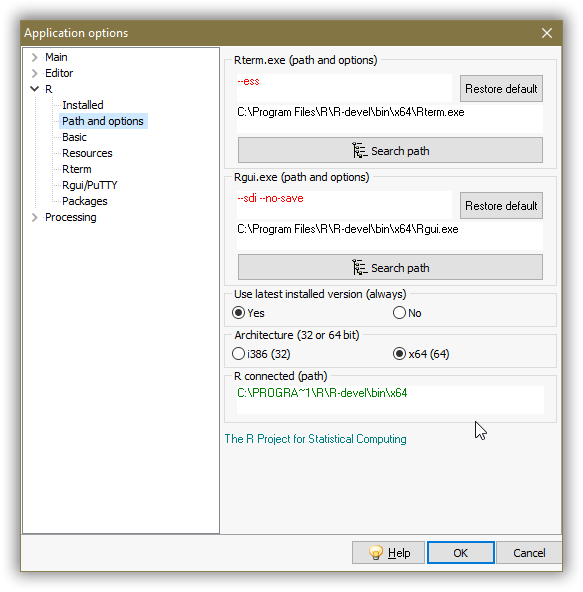
\includegraphics[scale=.50]{./res/app_r_pathandoptions.png}

\begin{itemize}
  \item You must start your preferred Rgui directly from Tinn-R. To do that,
    go to \texttt{Options/Application/R/Path}. \textbf{From Tinn-R version 8.02.01.01,
    Rgui must be launched from within Tinn-R so that it is properly
    identified at startup}.
  \item At the bottom of the dialog box, you can determine the path of
    the Rgui executable to start from within Tinn-R. Select
    \texttt{Rgui.exe} from, for instance,
    \texttt{C:$\backslash$Program Files$\backslash$R$\backslash$R-X.X.X$\backslash$bin$\backslash$Rgui.exe}).

    \begin{footnotesize}
      \begin{verbatim}
        Note: to use R from within Tinn-R, you must first install it from
        http://cran.r-project.org
      \end{verbatim}
    \end{footnotesize}

  \item With Rgui, you must choose SDI mode at Edit/GUI preferences.
\end{itemize}


\subsubsection{Can I define Tinn-R as the default editor for R objects?}
\index{FAQ!default editor}
\index{default editor}

\begin{itemize}
  \item No, currently, it does not have that capability. In order to do that,
    just use the internal script editor of Rgui to edit() or fix() \RR{} objects.
\end{itemize}


\subsubsection{Can I use Emacs or WinEdt style for syntax highlighting color?}
\index{FAQ!Emacs}
\index{Emacs}
\index{FAQ!WinEdt}
\index{WinEdt}

\begin{itemize}
  \item Just set your preferred color scheme in \texttt{Options/Colors (preference)}.
    To change color scheme on other computers, just use the
    \texttt{Options/Backup/Restore system options} configuration functions
    (\textit{\href{\#faq\_preferences}{See details ...}}).
\end{itemize}


\subsubsection{What does "Triggers" mean in Options/Application/R/General/Basic?}
\index{FAQ!triggers}
\index{triggers}

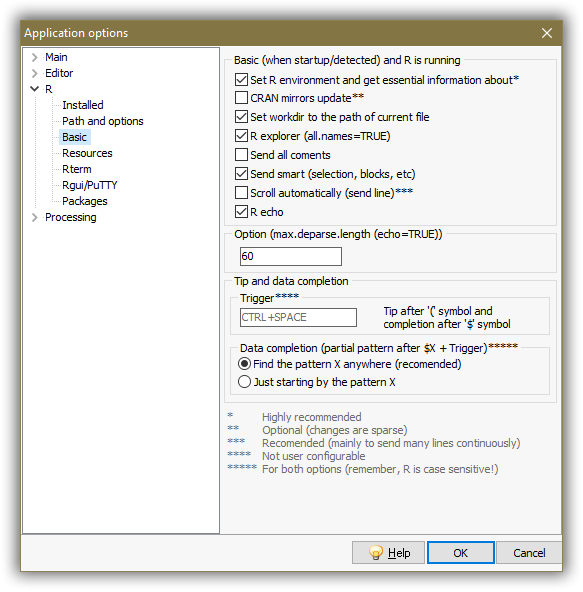
\includegraphics[scale=.50]{./res/app_r_basic.png}

\begin{itemize}
  \item Tips are tooltips displaying the syntax of the currently used
    \RR{} function.
  \item By default, if you enter the name of a function followed by an open
    bracket such as \texttt{sd(} in a \RR{} code document, then Tinn-R recognizes
    that you call the \texttt{sd} \RR{} function and reminds you of its syntax
    by showing the following tip: \texttt{x, na.rm=FALSE}, that is, \texttt{sd}
    accepts two arguments: \texttt{x}, and \texttt{na.rm} with the latter
    having \texttt{FALSE} as the default value.
  \item Tinn-R uses a database with the syntax of most common functions in \RR{}.
    However, neither functions in additional packages nor your custom
    functions are cached in this database.  Adding them all manually is
    tedious.
  \item Tinn-R therefore offers a second mechanism: direct requests to \RR{}. This
    is accomplished through DDE and/or TCP/IP protocols, using functions
    automatically loaded when you start the TinnR package you downloaded
    from CRAN.
    (\textit{\href{\#basic\_configuration}{See details ...}}).
  \item When a tip is showed (Editor, IO or LOG interface) it is possible
    to add all arguments by typing the shortcut \texttt{CTRL + *}.
\end{itemize}

On some computers, the delay for synchronization might need to be adjusted.
If Tinn-R seems to freeze while querying \RR{} for tips and you get no results,
increase the value a bit by setting
\texttt{Options/Application/Main/General/Computational synchronization (delay)}.


\subsubsection{Can I start R and Tinn-R all at once?}

\begin{itemize}
  \item There are many ways to accomplish this, but here is one: first,
    configure \RR{} so that it undersands that you want to use Tinn-R
    as your IDE (Integrated Development Environment). In order to do
    that, start a new \RR{} session and add the following command:

    \begin{footnotesize}
      \begin{verbatim}
        > options(IDE = "C:/Tinn-R/bin/Tinn-R.exe")
      \end{verbatim}
    \end{footnotesize}

    Replace the path by the present location of Tinn-R.exe on your computer
    if different from the location above. Then you will indicate that you
    want to start the DDE server automatically by setting (valid only for
    versions prior to 3.0.1.0, because this communication protocol
    was deleted from the project, the only one remaining is TCP/IP):

    \begin{footnotesize}
      \begin{verbatim}
        > options(use.DDE = TRUE)
      \end{verbatim}
    \end{footnotesize}


    At this point, Tinn-R will be automatically started when you load svIDE,
    at the same time as the \RR{} call-tip server is installed (valid only for
    versions prior to 3.0.1.0):

    \begin{footnotesize}
      \begin{verbatim}
        > library(TinnR)
      \end{verbatim}
    \end{footnotesize}

    If those steps work well in manual mode, but you now want them to run whenever
    you start \RR{}, edit the \texttt{Rprofile.site} file (located in the
    $\backslash$etc$\backslash$ subdirectory of \RR{}.  File location varies, but
    it should be under something like
    C:$\backslash$Program Files$\backslash$R$\backslash$R-X.X.X$\backslash$etc$\backslash$Rprofile.site).
    Add the above-mentioned three lines of code at the end of the Rprofile file (valid only for
    versions prior to 3.0.1.0).

    \begin{footnotesize}
      \begin{verbatim}
        options(IDE = "C:/Tinn-R/bin/Tinn-R.exe")
        options(use.DDE = TRUE)
        library(TinnR)
      \end{verbatim}
    \end{footnotesize}

    A copy of \texttt{Rprofile.site} file created by Jos� Cl�udio Faria can be obtained from
    \href{http://sourceforge.net/p/tinn-r/news/2013/01/rprofilesite-example/}{SourceForge},
    which you can adapt according to your needs. To make sure that everything works well and
    smoothly, close both \RR{} and Tinn-R and restart \RR{}. Tinn-R should start concomitantly.
    Now, create a very simple function in \RR{} such as:
    \index{installation!sourceforge}

    \begin{footnotesize}
      \begin{verbatim}
        > cube <- function(x) x^3
      \end{verbatim}
    \end{footnotesize}

    Switch to Tinn-R and type: \texttt{cube(}. You should get a call-tip displaying
    \texttt{x} if the \RR{} call-tip server was correctly installed.

\end{itemize}


\subsection{Hotkeys (operational system)}
\index{FAQ!hotkeys}
\index{hotkeys}

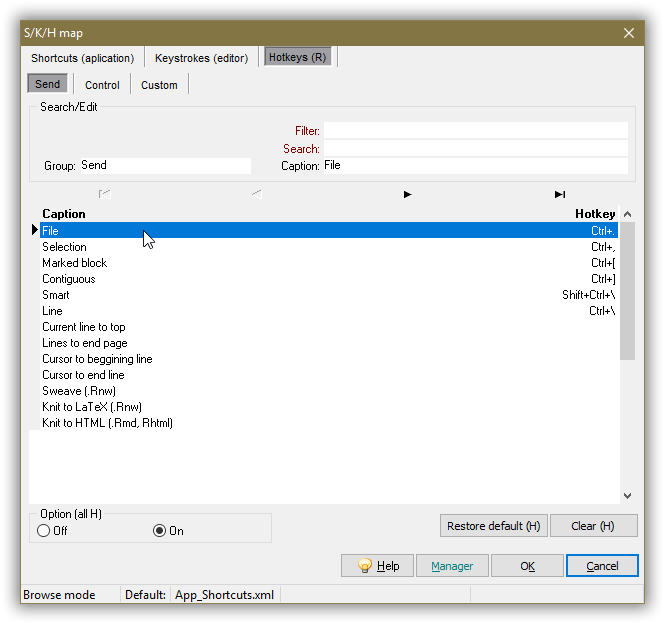
\includegraphics[scale=.40]{./res/skh_map_rh_send_dlg.png}
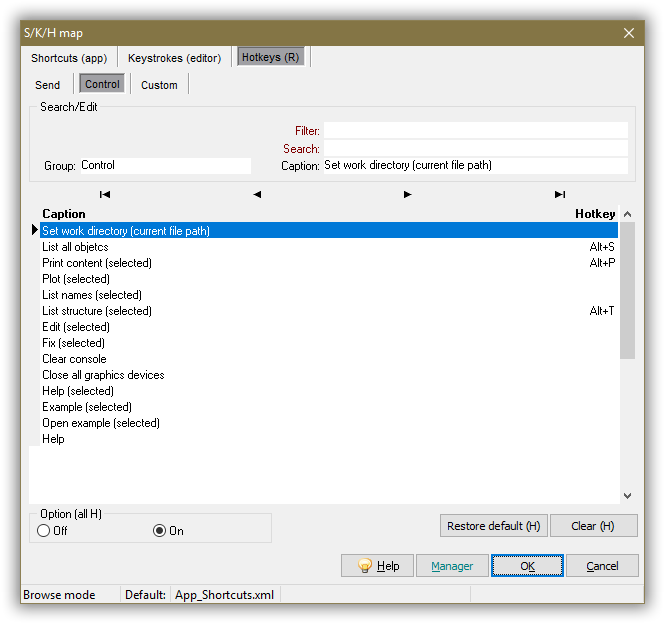
\includegraphics[scale=.40]{./res/skh_map_rh_control_dlg.png}
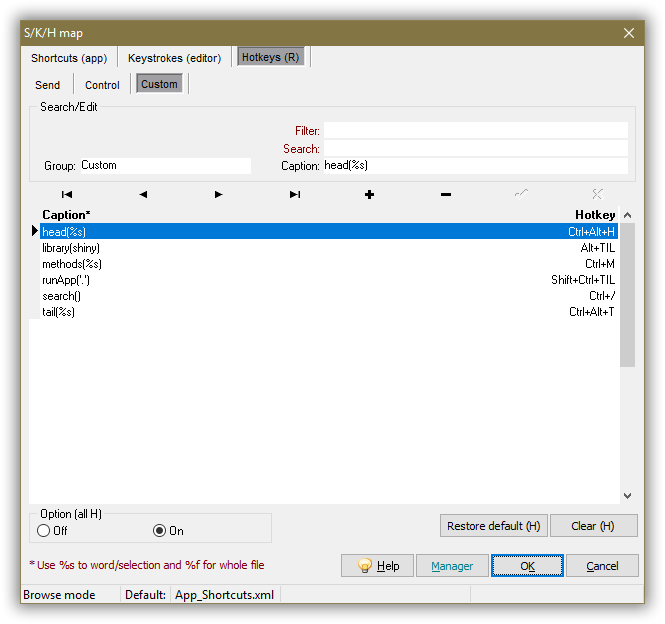
\includegraphics[scale=.40]{./res/skh_map_rh_custom_dlg.png}

\subsubsection{What is the difference between hotkeys (operational system) and shortcuts in Tinn-R?}

\begin{itemize}
  \item The hotkeys are related to the operational system. In other
    words, they work without the focus on Tinn-R, whereas the
    shortcuts will only work with the focus on the Tinn-R interface.
\end{itemize}


\subsubsection{How do I define hotkeys for R tools in Tinn-R?}
\index{FAQ!defining hotkeys}
\index{defining hotkeys}

\begin{itemize}
  \item Go to \texttt{R/Hotkeys of R}. Once there, define your favorite
    hotkeys for the various \RR{} tools and make sure to activate them
    (Option -$>$ Active).
\end{itemize}


\subsubsection{Is there a shortcut for cycling through opened files?}
\index{FAQ!shortcut for cycling}
\index{shortcut for cycling}

\begin{itemize}
  \item Yes, you can use \texttt{CTRL + TAB} to go to next file, and
    \texttt{CTRL + SHIFT + TAB} to go to previous ones when several
    files are loaded simultaneously in Tinn-R.
\end{itemize}


\subsubsection{Is there a shortcut for $<$- and -$>$ for the S/R languages?}

\begin{itemize}
  \item The (non user configurable) shortcut for \texttt{-$>$} is
    \texttt{CTRL + ADD} key (numeric keypad). Similarly,
    \texttt{CTRL + SUBTRACT} (numeric keypad) is a shortcut for
    \texttt{$<$-}. \texttt{-$>$} and \texttt{$<$-}, all being
    assignment symbols in the S/R languages.
\end{itemize}


\subsection{Miscellaneous}

\subsubsection{I am editing a table. Can I select text in column mode?}
\index{FAQ!column mode}
\index{column mode}

\begin{itemize}
  \item Yes you can, but you must first make sure that this option is selected.
    Go to \texttt{Options/Application/Editor/Advanced options} tab and check (x)
    \texttt{Alt sets column modes}. Once this is done, by pressing
    \texttt{Alt} key while selecting your text with the mouse in Tinn-R,
    the  selection will be done in column mode.
  \item Another option is to change the selection mode to column in a permanent
    way. This is done through the menu \texttt{Options/Selection mode} or by
    clicking on the selection mode place at the status bar. The available
    options are: \texttt{smNormal}, \texttt{smLine} and \texttt{smColumn}.
\end{itemize}


\subsubsection{Can I define bookmarks to facilitate the navigation through my documents?}
\index{FAQ!bookmarks}
\index{bookmarks}

\begin{itemize}
  \item Yes, you can define up to 10 bookmarks in each of your opened documents.
    To define the bookmark, use \texttt{CTRL + SHIFT + [0-9]} (a key from 0 to 9).
    Then, to go to the corresponding bookmark just use \texttt{CTRL + [0-9]}.
    A visual indicator appears in the right margin at the location of your
    bookmarks to remind you where they are.
\end{itemize}


\subsubsection{What is the left gutter used for?}
\index{FAQ!gutter}
\index{gutter}

\begin{itemize}
  \item In Tinn-R, bookmarks are visually displayed in the left gutter
    (use \texttt{CTRL + SHIFT + [0-9]} to set bookmarks and then use
    \texttt{CTRL + [0-9]} to navigate to them). It also displays the
    respective line numbers. You must set gutter \texttt{Visible} in
    \texttt{Options/Application/Editor/Display tab} (and also
    \texttt{Show line numbers}) to activate this feature.
\end{itemize}


\subsubsection{Can I run my code step-by-step?}
\index{FAQ!step-by-step}
\index{step-by-step}

\begin{itemize}
  \item Yes, but for more convenient use of this function, you must
    place Tinn-R and \RR{} side by side on your screen and click on the
    'Send line' icon with the mouse (seventh button from the left
    on the \RR{} toolbar).
  \item If you use a shortcut, you can just submit one line since the
    \RR{} console gets the focus when code is sent to \RR{}. Alternatively,
    you can set Tinn-R as a \texttt{topmost} window on top of \RR{}
    using \texttt{Options/On top}. The downside is that Tinn-R
    will permanently hide the \RR{} console and there is a chance
    that you won't see a part of the output generated in \RR{} during
    your step-by-step code execution.
\end{itemize}


\subsubsection{Is there a graphical debugger for my R functions?}
\index{FAQ!graphical debugger}
\index{graphical debugger}

\begin{itemize}
  \item Not yet, but you can download the excellent \texttt{debug}
    package from CRAN and use the \texttt{mtrace} function available
    from there.
\end{itemize}


\subsubsection{What is the Tools panel?}
\index{FAQ!tools panel}
\index{tools panel}

\begin{itemize}
  \item It is a panel you can open at either the left or the right
    side of your text. It helps you to manage large projects with
    multiple documents. The \texttt{Computer} tab allows you to
    explore your computer disks and open one or several files
    without using \texttt{File/Open}, or switching to the Windows
    file explorer. The \texttt{Project} tab is a convenient manager
    for all files collected in a given project.
\end{itemize}


\subsubsection{Can I copy and paste syntax highlighted R code in Word, Writer or other RTF edtitor?}
\index{FAQ!copy and paste}
\index{FAQ!copy and paste highlighted R code}
\index{FAQ!export syntax highlighted R code}
\index{copy and paste highlighted R code}
\index{export syntax highlighted R code}

\begin{itemize}
  \item Syntax highlighted code enhances the code's visibility. It is
    convenient in the code editor, but could also be useful for
    pieces of code presented elsewhere. Tinn-R allows you to copy the code while
    keeping syntax highlighting color through \texttt{Edit/Copy
    selection to clipboard (RTF formatted)}.
\end{itemize}


\subsubsection{How can I fix incorrect icon displays on Windows after I have installed a new version of Tinn-R?}
\index{FAQ!icon on Windows}
\index{icon on Windows}

\begin{itemize}
  \item If you get an incorrect icon displayed on Windows after
    installing a new version of Tinn-R, just proceed as follows:
    \begin{itemize}
      \item In order to accelerate the display of program or file
        icons, Windows stores images in the ICON CACHE (ShellIconCache),
        a hidden icon cache file in your Windows directory.
      \item Sometimes the icon of the object changes, but Windows still
        shows the old icon instead of the new one. To solve this
        problem, use the shareware program called
        \href{http://www.shelllabs.com/}{IconChanger}.
      \item If you have just installed Tinn-R with a new icon but Windows
        has not changed the image yet, use IconChanger and select REBUILD
        ICON CACHE.  If that still doesn't work, then select REMOVE ICON CACHE.
      \item If you have selected REBUILD the icon cache will start rebuilding
        from scratch. If you have selected REMOVE, you will see a warning
        message. Select YES and then restart your computer.
    \end{itemize}
\end{itemize}


\subsubsection{Basic instructions about focus control:}
\index{FAQ!focus control}
\index{focus control}

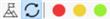
\includegraphics[scale=0.50]{./res/focus.png}
\begin{itemize}
  \item Tinn-R has a button within the \textit{Options toolbar}
    with the hint (\textit{Options: return focus to editor
      after send/control Rgui}) that enables the user to
    configure out the focus control. When this option is
    \texttt{checked} Tinn-R will display the following behavior:
    \begin{itemize}
      \item If the editor has the focus, it will \texttt{go back}
        to the editor after any \textit{send to} or \textit{R control}
        action, otherwise it will remain on Rgui. This is also
        true when working with a dual-monitor display.
    \end{itemize}
  \item If the Rterm has the focus, it will be \texttt{maintained}
    in this interface (\textit{IO}), \texttt{disregarding} the
    \textit{Options: return focus to editor after send/control
      Rgui}.
\end{itemize}


\subsubsection{Why Tinn-R doesn't remember my syntax color preferences?}\\
\index{FAQ!color preferences}
\index{color preferences}

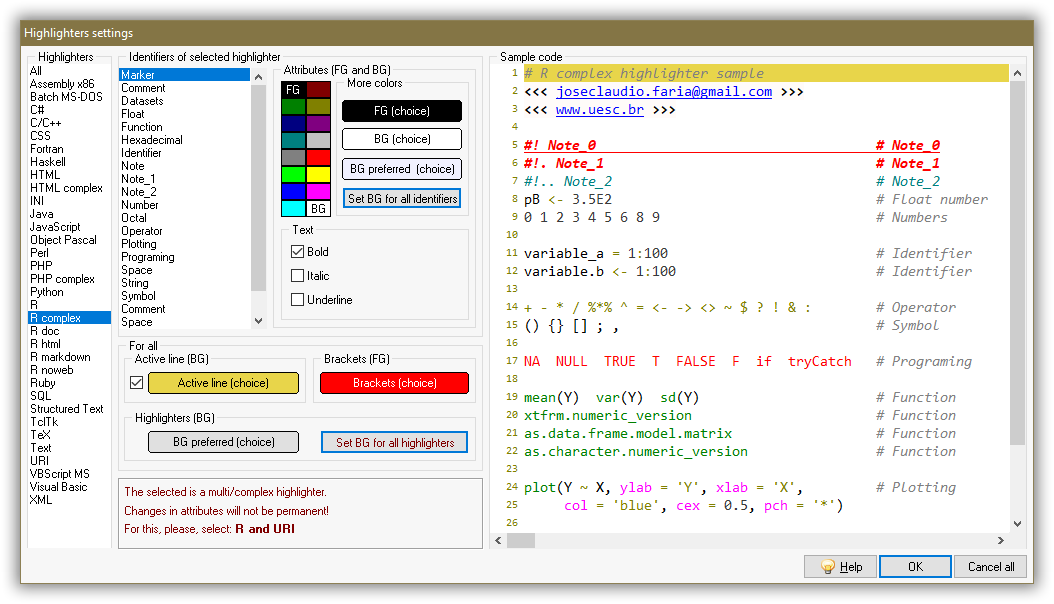
\includegraphics[scale=.50]{./res/highlighter_settings.png}

Tinn-R has seven multi-highlighters: \textit{HTML complex}, \textit{PHP complex},
\textit{R complex}, \textit{R doc},  \textit{R html}, \textit{R markdown} and \textit{R noweb},
with each one behaving as follows:

\begin{footnotesize}
  \begin{verbatim}
    1. HTML complex = HTML & JavaScript
    2. PHP complex  = HTML & JavaScript & PHP
    3. R complex    = R & URI ('<<<' begin URI; '>>>' end URI)
    4. R doc        = TeX & R ('>>=' begin R; '@' end R)
    5. R html       = HTML & R ('<!--begin.rcode' begin R; 'end.rcode-->' end R)
    5. R markdown   = URI & R ('```{' begin R; '```' end R)
    6. R noweb      = TeX & R ('>>=' begin R; '@' end R)

    URI       : Uniform Resource Identifiers.

    R complex : The main syntax is R, '<<<' and '>>>' are the tags enabling
                the user to insert a block of URI syntax.

    R doc     : The main syntax is TeX, '>>=' and '@' are the tags enabling
                the user to insert a block of R syntax.

    R html    : The main syntax is HTML, '<!--begin.rcode' and 'end.rcode-->' are the tags enabling
                the user to insert a block of R syntax.

    R markdown: The main syntax is URI, '```{' and '```' are the tags enabling
                the user to insert a block of R syntax.

    R noweb   : The main syntax is TeX, '>>=' and '@' are the tags enabling
                the user to insert a block of R syntax.

  \end{verbatim}
\end{footnotesize}

These highlighters do not establish priorities when you set the syntax color
preferences. Thus, if you change the color preferences for any of these
multi-highlighters these settings will be valid only
in the current Tinn-R session and will not be saved when Tinn-R is closed.
If you want to make these changes permanent, just set the  preferences
from all simple highlighters.


\subsubsection{How do I set a block as marked?}
\index{FAQ!marked blocks}
\index{marked blocks}

\begin{itemize}
  \item \textbf{If the file has no marks}: the option will not be
    available (grayed out);
  \item \textbf{If the file has one or more marks and the cursor
      is either above the first mark or below  the last mark}:
    all text (above or below this mark) will be submitted in
    relation to the cursor position (above or below) the mark;
  \item \textbf{If the cursor is between any two adjacent marks}:
    all text between those two marks will be submitted.
\end{itemize}


\subsubsection{How can I find errors in my script using Rterm interface?}
\index{FAQ!find errors in my script}
\index{find errors in my script}

\begin{itemize}
  \item The \texttt{Application options/R/Rterm} is split in two tabs: \texttt{Error} and \texttt{Options}.
    The tab Error has an option: \texttt{Trying to find code errors (at the editor)*}.
    It enables the user to set Tinn-R in order to find code errors at the editor when sending instructions to Rterm.
  \item It may happen that the error will not be found at the right place.
    For example, the error might be the same word
    appearing in a comment which comes before the actual code.
    In that case the user should use the shortcut \texttt{F3 (Find again)}.
    The word will appear selected, than just press \textit{OK} until finding the right error.
    The first search done internally by Tinn-R has \textit{Case sensitive} and \textit{Whole word only} as default,
    but, this is not passed to the search interface, therefore the user should just select them if convenient.
    If the error has numbers among letters \textit{Whole word only} is not a good option.
\end{itemize}


\subsubsection{The comunication between Tinn-R and Rgui.exe seems to freeze!}
\index{FAQ!comunication}
\index{comunication}
\index{FAQ!Tinn-R and Rgui}
\index{Tinn-R and Rgui}
\index{FAQ!freeze}
\index{freeze}

\begin{itemize}
  \item \textbf{First, it is not necessary to reinstall the Tinn-R nor R}!
  \item In some Windows flavors the communication between \texttt{Rgui} and \texttt{Tinn-R} sporadically seems to freeze.
    The cause of this bug is still unknown to us and seems to be related to the new features of some Windows flavors.
    However, the solution is very simple: rest your mouse (without pressing for a few seconds) on the
    icon of the Tinn-R on the taskbar of windows\ldots: the communication should be restored automatically.
\end{itemize}

\subsubsection{The comunication between Tinn-R and Rterm.exe seems to freeze using knit function!}
\index{FAQ!comunication}
\index{comunication}
\index{FAQ!Tinn-R and Rterm}
\index{Tinn-R and Rterm}
\index{FAQ!knitr}
\index{FAQ!knit}
\index{freeze}

\begin{itemize}
  \item To all \texttt{knit} procedures it will be added the argument \texttt{quiet=TRUE}.
    It is very dificult to sincronize the \texttt{txtProgreesBar} used in these functions and
    \texttt{Rterm} interface. So, if you want more control, we suggest (for while) to use the \texttt{knit}
    with \texttt{Rgui.exe} intead of \texttt{Rterm.exe}.
\end{itemize}

\subsubsection{How to make Ctrl+Shift+0 mark works?}
\index{FAQ!marks}
\index{FAQ!Ctrl+Shift+0}
\index{marks}
\index{Ctrl+Shift+0}

For Windows 10, do the following (it may be a bit different for Windows 8):
\begin{enumerate}
  \item In the control panel, click Language. This brings up the "Language" panel.
  \item Choose "Advanced Settings" in the left area. This brings up the "Advanced Settings" panel.
  \item Choose "Change language bar hot keys". This brings up the "Text Services \& Input Language" panel.
  \item Select that item and click the "Change Key Sequence" button. This brings up the "Change Key Sequence" panel.
  \item Set the Ctrl + Shift in both radio buttons to "Not Assigned" and click OK.
\end{enumerate}

           % Tinn-R Basics

% Experimental:
\renewcommand{\subsubsection} {\textsl{ }\\ }

\hypertarget{working}{}
\chapter{Working With}
This chapter provides information on how to work using Tinn-R.

\newpage

\hypertarget{working_app}{}
\section{Application options}
\index{application options}

\begin{figure}[H]
  \begin{center}
    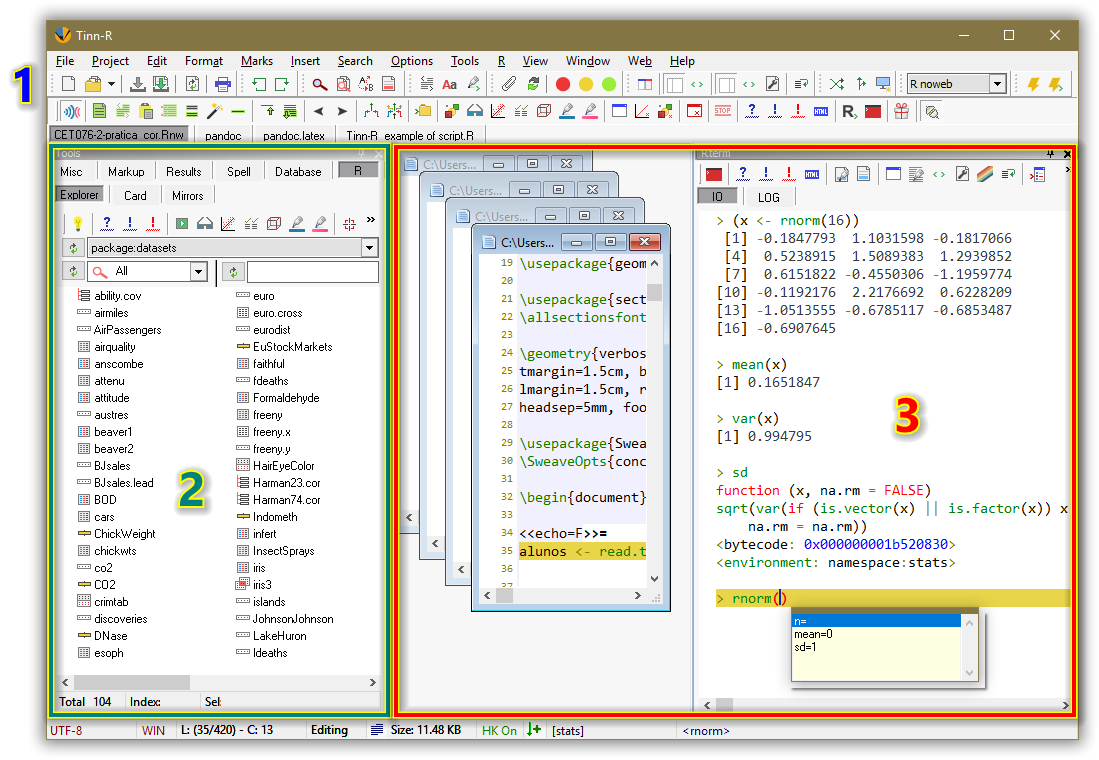
\includegraphics[width=\headwidth]{./res/parts_01.png}
  \end{center}
  \caption{Tinn-R: Main resources.}
  \label{fig:tinn-r_interface}
\end{figure}

Tinn-R interface
(Figure \ref{fig:tinn-r_interface})
is very flexible and user configurable. It is necessary time
to know all available resources and to configure this out (according to your
preferences) in a nice way. The default set of options might not be suitable
for every user.

The window \textit{Application options} allows the user to set the major piece
of user preferences related to the application.

It must be clear from now on that the Tinn-R project is the sum of three main
resources (Figure \ref{fig:tinn-r_interface}):
The application \texttt{per se (1)},
additional \texttt{Tools (2)} and
the instances of the \texttt{SynEdit class (3)}.
The \texttt{Tools (2)} was projected to allows the expansion of resources.
\index{application options}

The options visible in all pictures reflect a set of the project leader preferences.


\hypertarget{working_app_main}{}
\subsection{Main}
\index{application options!main}

\begin{figure}[H]
  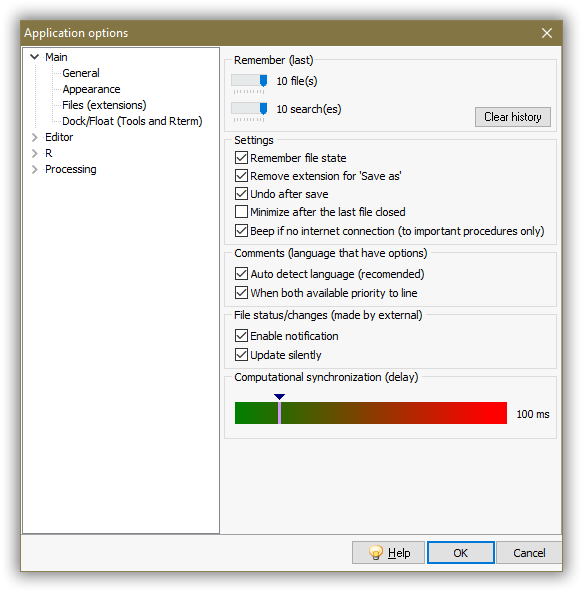
\includegraphics[scale=0.35]{./res/app_main_general.png}~~
  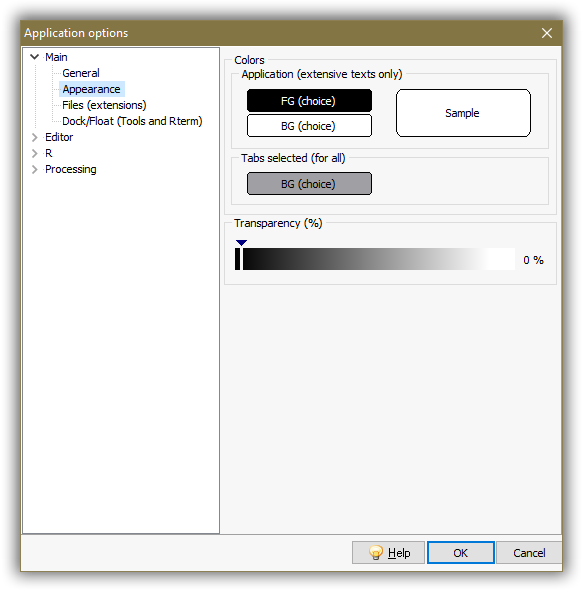
\includegraphics[scale=0.35]{./res/app_main_appearance.png}\\
  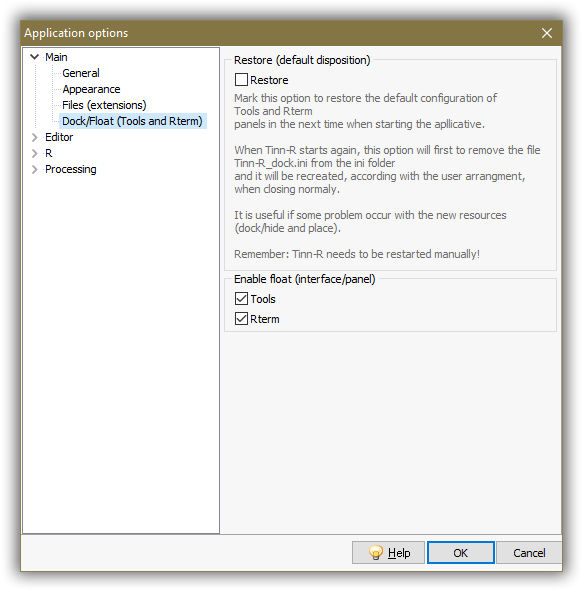
\includegraphics[scale=0.35]{./res/app_main_dock.png}~~
  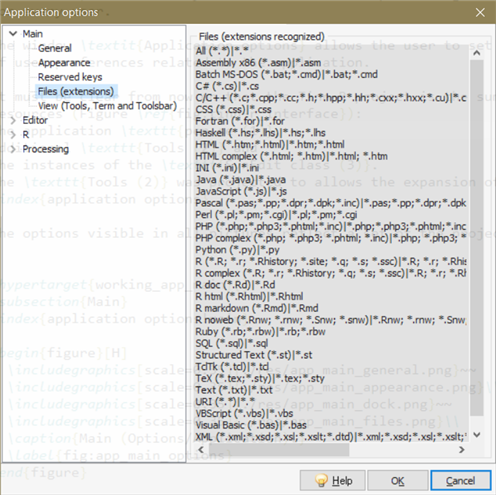
\includegraphics[scale=0.35]{./res/app_main_files.png}\\
  \caption{Main (Options/Application).}
  \label{fig:app_main_options}
\end{figure}

\begin{table}
  \begin{footnotesize}
    \begin{tabularx}{\headwidth}{>{\hsize=0.35\hsize}X>{\hsize=0.65\hsize}X}\\
      \hline
      \textbf{Option} & \textbf{Description} \\
      \hline
      Computational syncronization (delay) & Several processes are dependent on synchronization between applications
       (\RR{}, converters, compilers). The optimal value of the delay is determined by the following characteristics:
       user habits, hardware and software available.
       The ideal value is unique to the various possible combinations of those three characteristics.
       Try to reduce to the minimum value (50 ms) and test it: if something does not work, increase it gradually
       and keep testing until getting to the optimal value. The default value (100 ms) may not be optimal for all users. \\
      Remove extension for \textit{Save as} & All file extensions will be removed
       in the \textit{Save as} Windows interface \\
      Application colors (extensive text only) & Dark colors (low level of radiation)
       for the background, and pale light (high level of radiation) for the characters
       are reccomended for people who work with the computer/monitor for long periods.
       Pictures of this user guide ire like this \\
      \hline
    \end{tabularx}
  \end{footnotesize}
  \caption{Same main options}
  \label{tab:app_main}
\end{table}

Figure \ref{fig:app_main_options} and
Table \ref{tab:app_main}
show the options related to this topic.

Since the options are self-explanatory, Table \ref{tab:app_main} only gives some
details about the most difficult options to understand.


\hypertarget{working_editor}{}
\subsection{Editor}
\index{application options!editor}

The \textit{Editor} window
(Figures \ref{fig:editor_display}, \ref{fig:editor_advanced})
was adapted from the sources of the
\textit{SynEdit} component, mainly related to the general appearance and
standard options. The set of options available complement the
\textit{Application options} and allows high level of customization.


\hypertarget{working_editor_display}{}
\subsubsection{Display:}
\index{application options!!editor display}

\begin{figure}[H]
  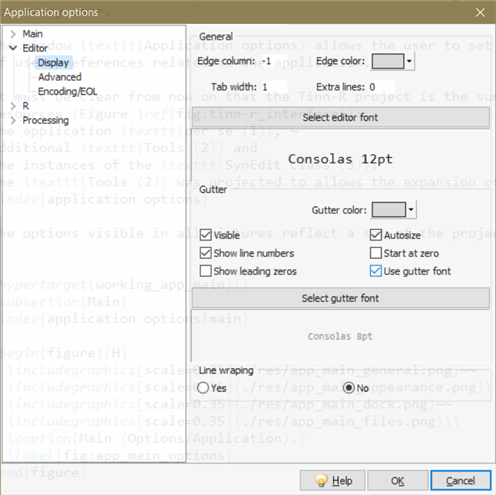
\includegraphics[scale=0.50]{./res/app_editor_display.png}~~
  \caption{Editor options: Display.}
  \label{fig:editor_display}
\end{figure}

\begin{table}
  \begin{footnotesize}
    \begin{tabularx}{\textwidth}{>{\hsize=0.3\hsize}X>{\hsize=0.7\hsize}X}\\
      \hline
      \textbf{Option} & \textbf{Description} \\
      \hline  %Display-----
      Edge column & Will be showed as a vertical line in the editor and the default is 80 characters.
      Set it to 0 or a negative value (-1) to make the edge column not visible \\
      Edge color & Choice of the edge color \\
      Tab width & Set the number of characters that will be inserted when typing the \textit{Tab} key \\
      Extra lines & Set the width which each single line will be displayed \\
      Font & Will open the Windows interface for choosing installed fonts \\
      \hline %Gutter-----
      Gutter color & Will open the Windows interface to choose a color \\
      Visible & Visibility option \\
      Autosize & Autosize option \\
      Show line number & Show line number option \\
      Start at zero & Start at zero option \\
      Show leading zeros & Show leading zeros option \\
      Use gutter font & Use gutter font option \\
      \hline
    \end{tabularx}
  \end{footnotesize}
  \caption{Display (Options/Editor).}
  \label{tab:editor_display}
\end{table}

Figure \ref{fig:editor_display} and
Table \ref{tab:editor_display}
show the main resources.

\hypertarget{working_editor_advanced}{}
\subsubsection{Advanced:}
\index{application options!editor advanced}

\begin{figure}[H]
  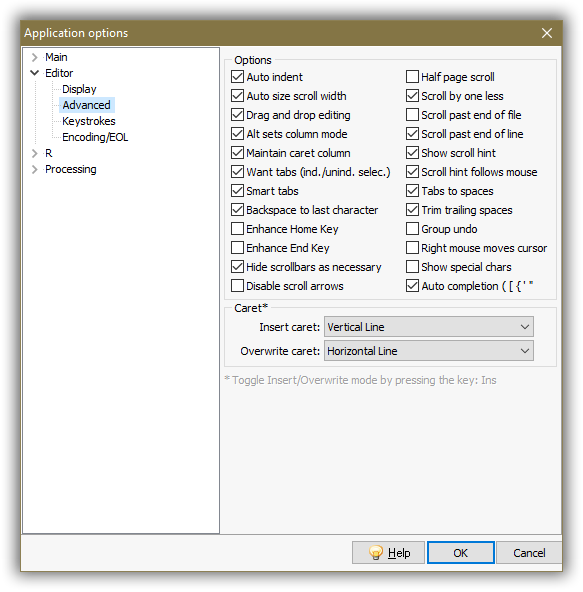
\includegraphics[scale=0.50]{./res/app_editor_advanced.png}~~
  \caption{Editor options: Advanced.}
  \label{fig:editor_advanced}
\end{figure}

\begin{table}
  \begin{footnotesize}
    \begin{tabularx}{\headwidth}{lX}\\
      \hline
      \textbf{Option} & \textbf{Description} \\
      \hline %Options-----
      Auto indent & Will indent the caret (position of the cursor in the current line) on new lines with the same amount of leading white space as the preceding line \\
      Auto size scroll width & Automatically resizes the MaxScrollWidth property when inserting text \\
      Drag and drop editing & Allows you to select a block of text and drag it within the document to another location \\
      Alt sets column mode & Holding down the $<$ALT$>$ key will put the selection mode into column format \\
      Maintain caret column & When moving through lines w/o cursor past EOL, keeps the X position of the cursor \\
      Want tabs (ind./unind. select.) & When tabbing (if there is a selection) $<$TAB$>$ and $<$SHIFT$>$$<$TAB$>$ act as block indent, unindent \\
      Smart tabs & When tabbing, the cursor will go to the next non-white space character of the previous line \\
      Backspace to last character & The cursor will go to the next non-white space character of the line \\
      Enhance home key & Enhances HOME key positioning, similar to visual studio \\
      Enhance end Key & Enhances END key positioning, similar to JDeveloper \\
      Hide scrollbars as necessary & If enabled, then the scrollbars will only show when necessary.
      If you have ScrollPastEOL, then the horizontal bar will always be there (it uses MaxLength instead) \\
      Disable scroll arrows & Disables the scroll bar arrow buttons when you can't scroll in that direction any more \\
      Half page scroll & When scrolling with page-up and page-down commands, only scroll a half page at a time \\
      Scroll by one less & Forces scrolling to be one less \\
      Scroll past end of file & Allows the cursor to go past the end of file marker \\
      Scroll past end of line & Allows the cursor to go past the last character into the white space at the end of a line \\
      Show scroll hint & Shows a hint of the visible line numbers when scrolling vertically \\
      Scroll hint follows mouse & The scroll hint follows the mouse when scrolling vertically \\
      Tabs to spaces & Converts a tab character to a specified number of space characters \\
      Trim trailing spaces & Spaces at the end of lines will be trimmed and not saved \\
      Group undo & When undoing/redoing actions, handle all continuous changes of the same kind in one call instead undoing/redoing
      each command separately \\
      Right mouse moves cursor & When clicking with the right mouse for a pop-up menu, move the cursor to that location \\
      Show special chars & Shows the special characters \\
      \hline %Caret-----
      Insert caret & A list with four options: Vertical line, Horizontal line, Half block and block \\
      Overwrite caret & A list with options: Vertical line, Horizontal line, Half block and block \\
      \hline
    \end{tabularx}
  \end{footnotesize}
  \caption{Display (Options/Editor).}
  \label{tab:editor_advanced}
\end{table}

Figure \ref{fig:editor_advanced} and
Table \ref{tab:editor_advanced}
show the main resources.


\hypertarget{working_editor_encoding_eol}{}
\subsubsection{Encoding/EOL:}
\index{application options!editor encoding}
\index{application options!editor EOL}

\begin{figure}[H]
  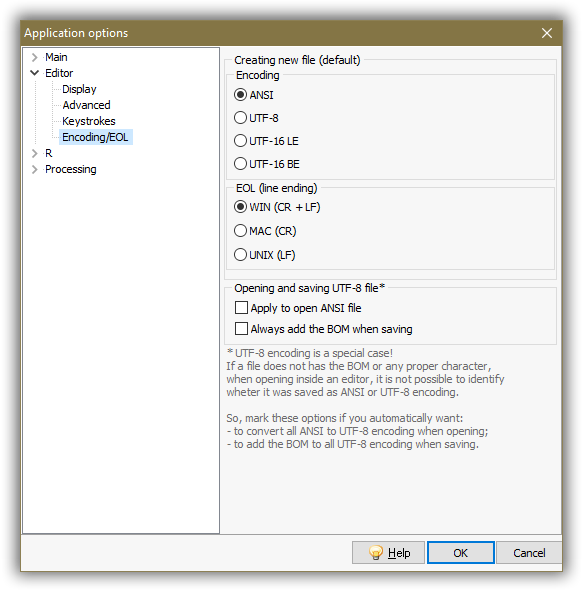
\includegraphics[scale=0.50]{./res/app_editor_encoding.png}\\
  \caption{Editor options: encoding/EOL.}
  \label{fig:editor_encoding}
\end{figure}

This interface
(Figure \ref{fig:editor_encoding})
allows to change the default encoding and EOL when creating new files and
also the user option related to UTF-8 files.


\hypertarget{working_app_r}{}
\subsection{R}
\index{application options!R}

\begin{figure}[h!]
  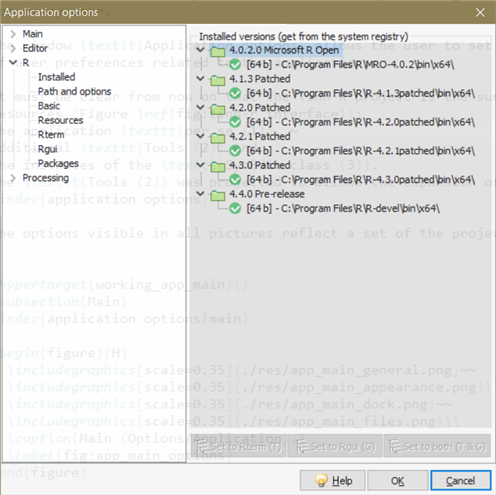
\includegraphics[scale=0.35]{./res/app_r_installed.png}~~
  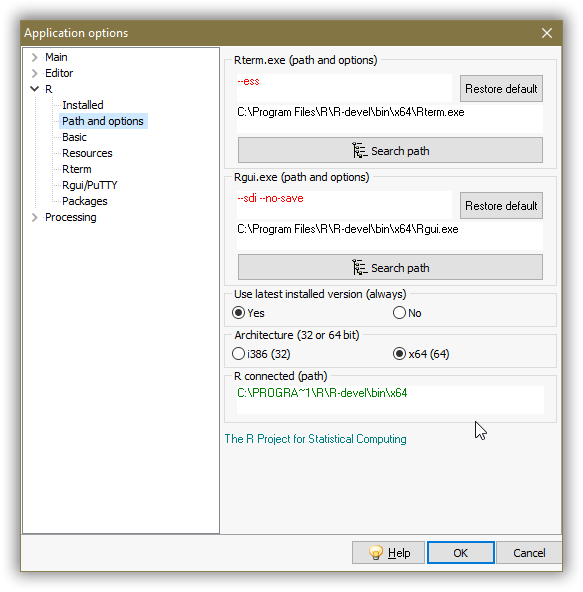
\includegraphics[scale=0.35]{./res/app_r_pathandoptions.png}\\
  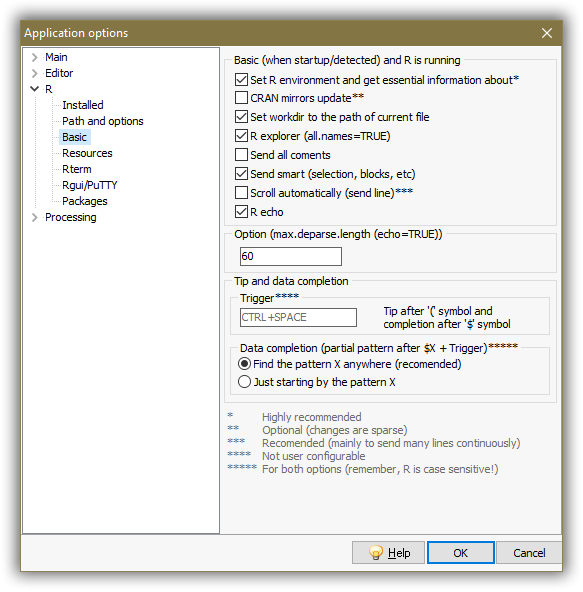
\includegraphics[scale=0.35]{./res/app_r_basic.png}~~
  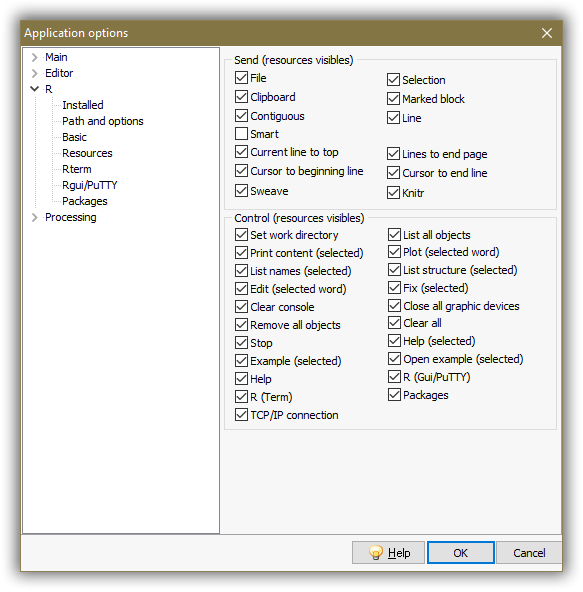
\includegraphics[scale=0.35]{./res/app_r_resources.png}\\
  \caption{R (Options/Application).}
  \label{fig:app_r_a}
\end{figure}

\begin{figure}[h!]
  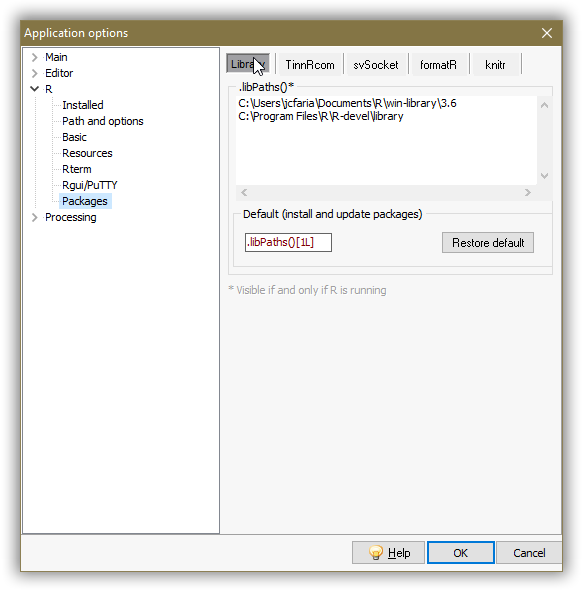
\includegraphics[scale=0.33]{./res/app_r_packages_library.png}~~
  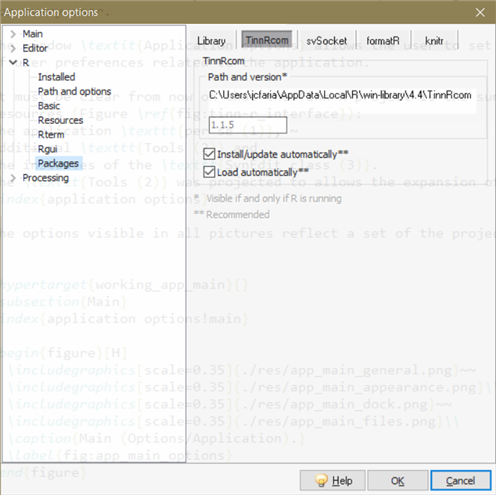
\includegraphics[scale=0.33]{./res/app_r_packages_tinnrcom.png}\\
  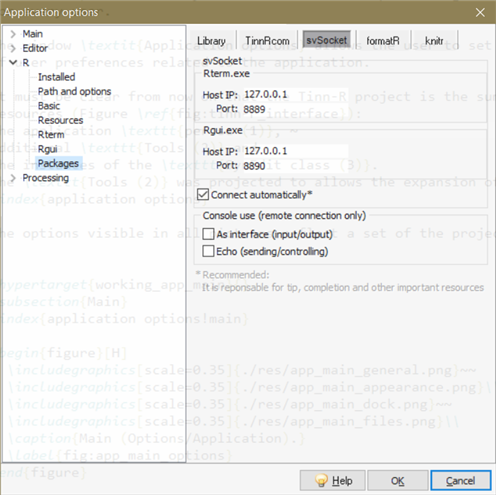
\includegraphics[scale=0.33]{./res/app_r_packages_svsocket.png}\\
  \caption{R (Options/Application).}
  \label{fig:app_r_b}
\end{figure}

\begin{figure}[h!]
  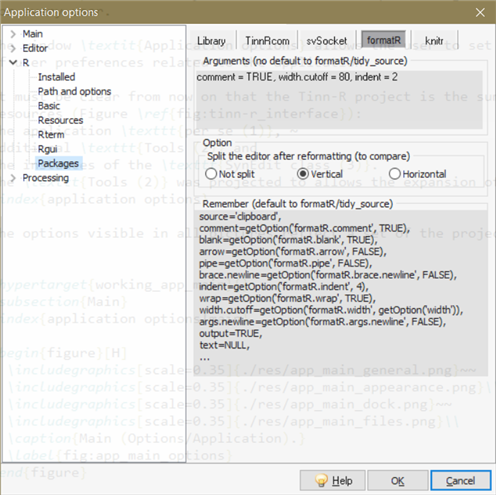
\includegraphics[scale=0.33]{./res/app_r_packages_formatr.png}~~
  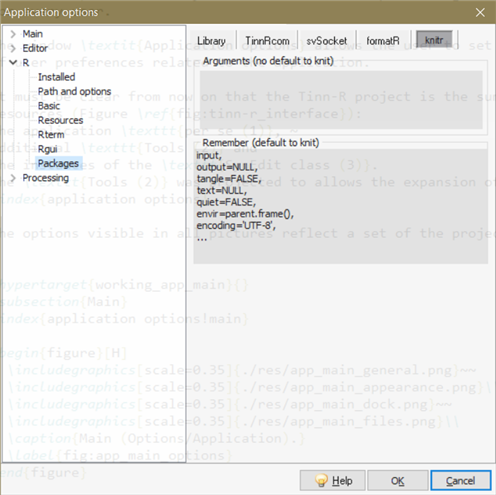
\includegraphics[scale=0.33]{./res/app_r_packages_knitr.png}\\
  \caption{R (Options/Application).}
  \label{fig:app_r_c}
\end{figure}

\begin{figure}[h!]
  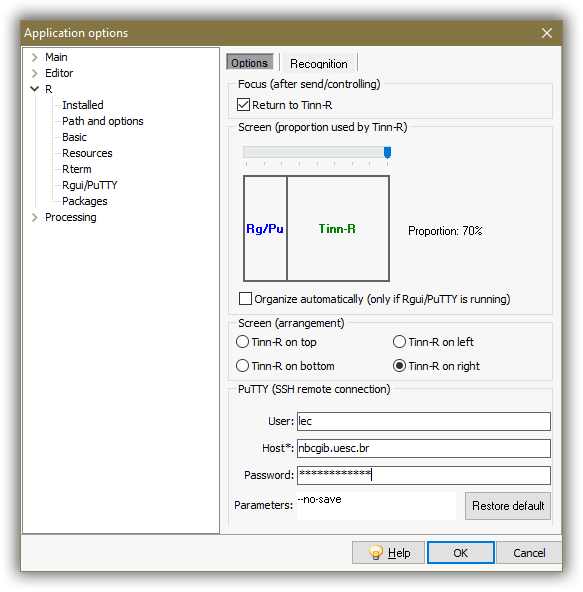
\includegraphics[scale=0.35]{./res/app_r_rgui_options.png}~~
  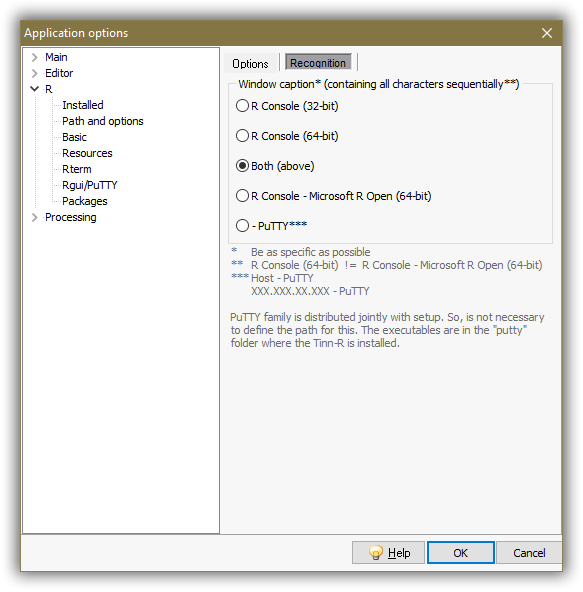
\includegraphics[scale=0.35]{./res/app_r_rgui_recognition.png}\\
  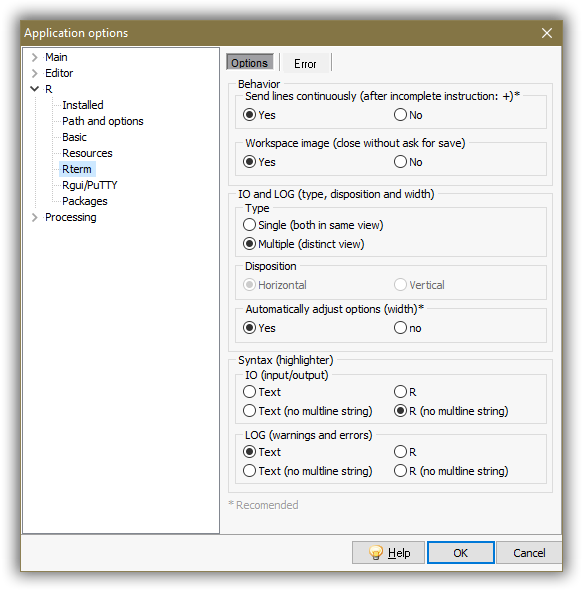
\includegraphics[scale=0.35]{./res/app_r_rterm_options.png}~~
  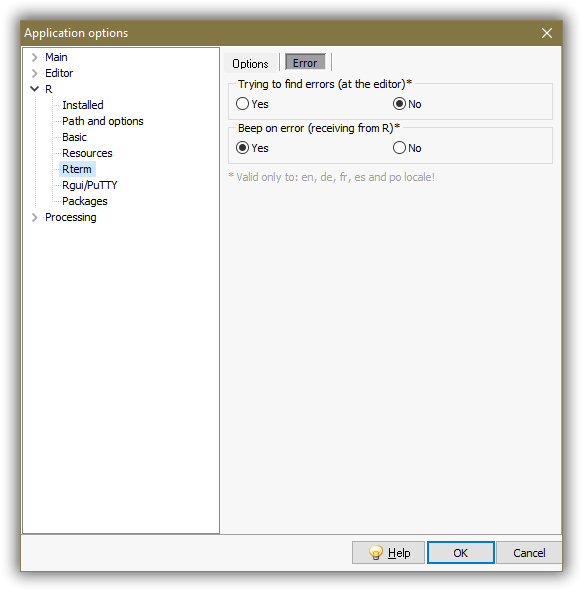
\includegraphics[scale=0.35]{./res/app_r_rterm_error.png}\\
  \caption{R (Options/Application).}
  \label{fig:app_r_d}
\end{figure}

Figures \ref{fig:app_r_a},
        \ref{fig:app_r_b},
        \ref{fig:app_r_c} and
        \ref{fig:app_r_d}
shows a set of options available. As you can see, it allows a high level
of customization with the \RR{} environment.


\hypertarget{working_app_processing}{}
\subsection{Processing}
\index{application options!processing}

\begin{figure}[h!]
  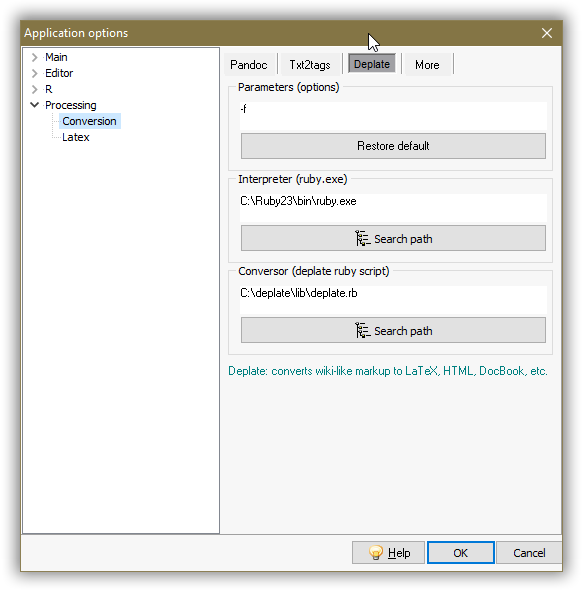
\includegraphics[scale=0.35]{./res/app_processing_conversion_deplate.png}~~
  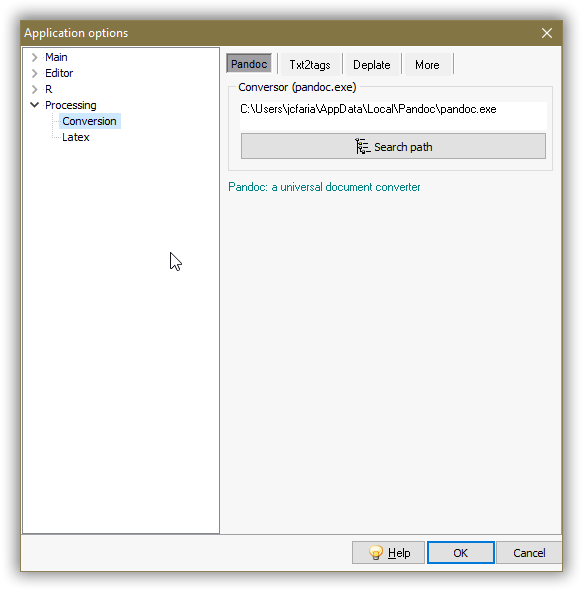
\includegraphics[scale=0.35]{./res/app_processing_conversion_pandoc.png}\\
  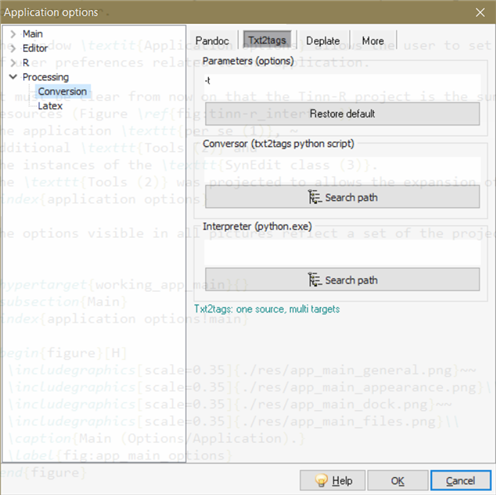
\includegraphics[scale=0.35]{./res/app_processing_conversion_txt2tags.png}~~
  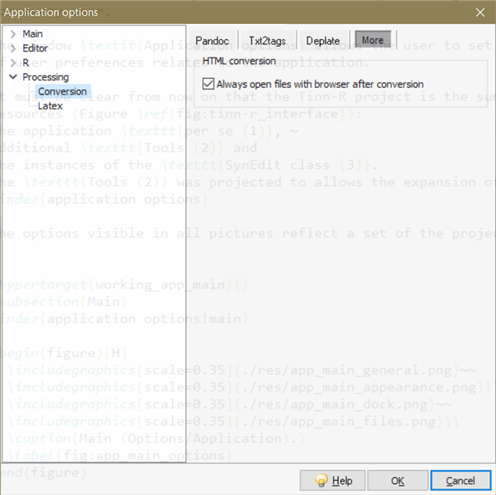
\includegraphics[scale=0.35]{./res/app_processing_conversion_more.png}\\
  \caption{Conversion (Options/Application/Processing).}
  \label{fig:app_processing_conversion_options}
\end{figure}

There are resources
(Figure \ref{fig:app_processing_conversion_options} and
\ref{fig:app_processing_latex_options})
related to conversion (Deplate, Pandoc and Txt2tags) and compilation (Miktex).


\hypertarget{working_app_processing_conversion}{}
\subsubsection{Conversion:}
\index{application options!processing conversion}

Tinn-R project makes it easy to work with these nice conversion tools: Deplate, Pandoc and Txt2tags.
(Figure \ref{fig:app_processing_conversion_options}).


%\newpage
\hypertarget{working_app_processing_latex}{}
\subsubsection{LaTex:}
\index{application options!processing LaTeX}

\begin{figure}[h!]
  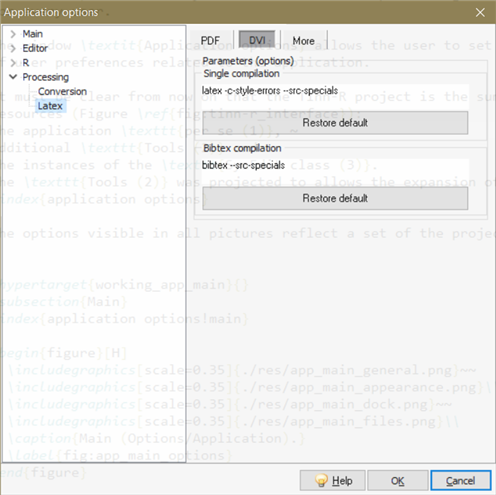
\includegraphics[scale=0.33]{./res/app_processing_latex_dvi.png}~~
  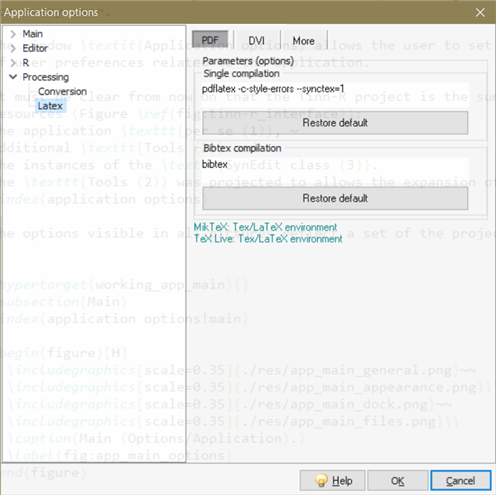
\includegraphics[scale=0.33]{./res/app_processing_latex_pdf.png}\\
  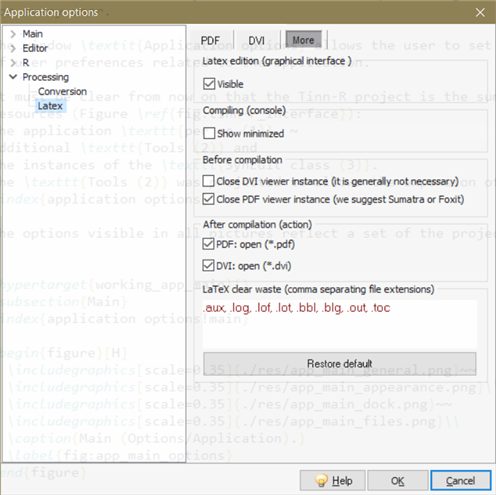
\includegraphics[scale=0.33]{./res/app_processing_latex_more.png}\\
  \caption{Latex (Options/Application/Processing).}
  \label{fig:app_processing_latex_options}
\end{figure}

Tinn-R is not a specific editor to \LaTeX, but it has the basic resources (Figure \ref{fig:app_processing_latex_options}) allowing the user to use the main resources of this environment.

\newpage

\hypertarget{working_selectionmode}{}
\section{Selection mode}
\index{selection mode}

Allows the setting of the current selection mode
(Figure \ref{fig:selection_normal},
\ref{fig:selection_line} and
\ref{fig:selection_column}).

Select text by clicking and dragging with the left mouse button held
down or moving the cursor with the shift key held down. The status
bar will display an icon indicating the current selection mode.

\hypertarget{working_selectionmode_normal}{}
\subsection{Normal}
\index{selection mode!normal}

\begin{figure}[H]
  \includegraphics[scale=0.35]{./res/selection_normal.png}\\
  \caption{Normal (selection mode).}
  \label{fig:selection_normal}
\end{figure}

This is the standard selection mode
(Figure \ref{fig:selection_normal})
found in many Windows applications.

\hypertarget{working_selectionmode_line}{}
\subsection{Line}
\index{selection mode!line}

\begin{figure}[H]
  \includegraphics[scale=0.35]{./res/selection_line.png}\\
  \caption{Line (selection mode).}
  \label{fig:selection_line}
\end{figure}

This selection mode
(Figure \ref{fig:selection_line})
allows only for complete lines to be selected.

\hypertarget{working_selectionmode_column}{}
\subsection{Column}
\index{selection mode!column}

\begin{figure}[H]
  \includegraphics[scale=0.35]{./res/selection_column.png}\\
  \caption{Column (selection mode).}
  \label{fig:selection_column}
\end{figure}

This selection mode
(Figure \ref{fig:selection_column})
allows vertical blocks of text to be selected.
The option \texttt{ALT} sets column mode allowing the selection
mode to be switched to Column Mode when selecting with the mouse
by simply holding down the \texttt{ALT} key.
\href{\#working_editor_advanced}{See details at editor (advanced options)}.

\newpage

\hypertarget{working_highlighters}{}
\section{Highlighters (settings)}
\index{highlighters!color}

\begin{figure}[H]
  \includegraphics[scale=0.50]{./res/dlg_highlighter_settings.png}\\
  \caption{Highlighter preferences.}
  \label{fig:highlighter_preferences}
\end{figure}

This interface
(Figure \ref{fig:highlighter_preferences})
allows you to customize the appearance and colors of the
instances of the class \textit{SynEdit} (Editor, IO and LOG).

The interface is simple and self-explanatory.

Basically, make a choice between the set of highlighters available
from the \textit{Highlighters} list. The identifier of the selected
highlighter will be updated. It is possible to set only one
foreground attribute each time. But it is possible to set the
background for all attributes of the selected highlighter and also
the background of all attributes of all highlighters.

It is also possible to set the color brackets and the active line
background.


\subsubsection{Observation:}\\
\index{highlighters!multi-highlighters}

Tinn-R has seven multi-highlighters: \textit{HTML complex}, \textit{PHP complex},
\textit{R complex}, \textit{R doc},  \textit{R html}, \textit{R markdown} and \textit{R noweb},
with each one behaving as follows:

\begin{footnotesize}
  \begin{verbatim}
    1. HTML complex = HTML & JavaScript
    2. PHP complex  = HTML & JavaScript & PHP
    3. R complex    = R & URI ('<<<' begin URI; '>>>' end URI)
    4. R doc        = TeX & R ('>>=' begin R; '@' end R)
    5. R html       = HTML & R ('<!--begin.rcode' begin R; 'end.rcode-->' end R)
    5. R markdown   = URI & R ('```{' begin R; '```' end R)
    6. R noweb      = TeX & R ('>>=' begin R; '@' end R)

    URI       : Uniform Resource Identifiers.

    R complex : The main syntax is R, '<<<' and '>>>' are the tags enabling
                the user to insert a block of URI syntax.

    R doc     : The main syntax is TeX, '>>=' and '@' are the tags enabling
                the user to insert a block of R syntax.

    R html    : The main syntax is HTML, '<!--begin.rcode' and 'end.rcode-->' are the tags enabling
                the user to insert a block of R syntax.

    R markdown: The main syntax is URI, '```{' and '```' are the tags enabling
                the user to insert a block of R syntax.

    R noweb   : The main syntax is TeX, '>>=' and '@' are the tags enabling
                the user to insert a block of R syntax.

  \end{verbatim}
\end{footnotesize}

These highlighters haven't priorities when you set the syntax color preferences.
Thus, if you change the colors' preferences of any of these multi-highlighters
these settings will be valid only in the current Tinn-R session and will not be
saved when Tinn-R is closed. So, if you want to make permanent changes, set the
preferences from all simple highlighters.

From version 3.0.1.0 a warning message is displayed whenever
a multi-highlighter is selected. It shows which highlighters the user
must change the characteristics so that they are properly stored and
henceforth always displayed.

\newpage

\hypertarget{working_shortcuts}{}
\section{Shortcuts (Application)}
\index{shortcuts}
\index{shortcuts!application}

\begin{figure}[H]
  \includegraphics[scale=0.40]{./res/shortcuts_dlg.png}\\
  \caption{Shortcuts customization.}
  \label{fig:shortcuts_dlg_1}
\end{figure}

The \textit{Shortcuts customization}
(Figure \ref{fig:shortcuts_dlg_1})
allows the user to set the shortcuts related
to the application, it works together with the \textit{Editor keystrokes},
and allows for high level of customization.

The difference between \textit{Shortcuts} and \textit{Hotkeys (operational system)}
is that the former works only with the focus on Tinn-R, whereas hotkeys work
with the focus anywhere.

Read below a brief description of available buttons.

\begin{quote}
  \begin{footnotesize}
    \begin{description}
      \item[Restore default:]
        Restores the file \texttt{Shortcuts.xml} from the origin
        (InstallPath/data/data.zip). Any prior changes to the file
        \texttt{Shortcuts.xml} in use will be lost.
      \item[Save as default:]
        Opens the save dialog allowing to save the file. From this
        point, this file will be the new default shortcuts.
      \item[Load:]
        Opens the open dialog allowing to load a shortcut file. From this
        point on, this file will be the new default shortcuts.
      \item[Edit:]
        Sets the table in edition mode.
      \item[Cancel current:]
        Cancels any changes made to the current edition.
      \item[Cancel all:]
        Cancels all changes made to the database prior to \textit{Save}
        or \textit{Save as default}.
      \item[Save:]
        Saves to text file (XML) all changes made to the current table.
      \item[Close:]
        Closes the dialog. All changes not saved will be lost.
    \end{description}
  \end{footnotesize}
\end{quote}

\newpage

\hypertarget{working_editor}{}
\section{Keystrokes (Editor)}
\index{editor}
\index{editor!keystrokes}

\begin{figure}[H]
  \includegraphics[scale=0.35]{./res/skh_map_keystrokes_dlg.png}\\
  \caption{Keystrokes (Databases).}
  \label{fig:keystrokes_dlg}
\end{figure}

This interface
(Figure \ref{fig:keystrokes_dlg})
allows to change the default SynEdit keystrokes.
It is possible only change the keystroke associaed to any \texttt{ecAction} (execute command action).
A set of user friendly keystrokes gives high productivity leading with
all instances of the class \textit{SynEdit}: Editor, IO and LOG.

Read below for a brief description of available buttons (Figure \ref{fig:keystrokes_dlg}):

\begin{quote}
  \begin{footnotesize}
    \begin{description}
      \item[Restore default (K):]
        Restores the file \texttt{Editor\_Keystrokes.xml} from the origin at
        (\texttt{InstallPath/data/data.zip}). Any prior change to the file ini file
        \texttt{Editor\_Keystrokes.xml} being used will be lost.
      \item[Clear (K):]
        Clear the selected keystroke.
    \end{description}
  \end{footnotesize}
\end{quote}

\newpage

\hypertarget{working_hotkeys}{}
\section{Hotkeys (R Send/Control/Custom)}
\index{hotkeys}

\begin{figure}[H]
  \includegraphics[scale=0.36]{./res/skh_map_rh_send_dlg.png}
  \includegraphics[scale=0.36]{./res/skh_map_rh_control_dlg.png}
  \includegraphics[scale=0.36]{./res/skh_map_rh_custom_dlg.png}
  \caption{Hotkeys.}
  \label{fig:hotkeys}
\end{figure}

The \textit{Hotkeys (operational system)}
(Figure \ref{fig:hotkeys})
allow setting the hotkeys
related to the operational system. The difference between those hotkeys and
\textit{Shortcuts customization} is that the latter works only with the
focus in Tinn-R, whereas the hotkeys work with the focus anywhere.

The interface is self-explanatory. Basically you first make a choice from
the \textit{R/Hotkeys (operational system)} and set the desired Hotkey.

The set of hotkeys will perform actions only if the option \textit{Active}
is checked. The objective of these options (\textit{Inactive} and
\textit{Active}) is to avoid conflict with others applications allowing
to enable/disable the set of hotkeys quickly and easily.

The \texttt{R/Hotkeys} interface was deeply reworked in the version 5.05.01.01 and it now has three tabs,
\texttt{Send}, \texttt{Control} and \texttt{Custom}:

\begin{itemize}
\item \texttt{Send}: Contains the already traditional \texttt{Send} instructions of Tinn-R;
\item \texttt{Custom}: Contains the already traditional \texttt{Control} instructions of Tinn-R;
\item \texttt{Custom}: \textbf{Allows the user to customize any instructions} to be send to \RR{} interpreter (thanks to Philemon Lenherr for the suggestion). The instructions must be as follows:
 \begin{itemize}
 \item Simple: \texttt{search()}. The \RR{} interpreter will receive \texttt{$>$ search()};
 \item Replace word or small selection: \texttt{View(\%s, title='View of iris dataset')}.
   If the editor cursor is over the word \texttt{iris} or it is selected,
   the \RR{} interpreter will receive \texttt{$>$ View(iris, title='View of iris dataset')}
 \item Replace whole file: \texttt{source(\%f, echo=TRUE, verbose=TRUE)}.
   The \RR{} interpreter will receive \texttt{$>$ source(.trPaths[4], echo=TRUE, verbose=TRUE)}.
   All rules related to send file are preserved.
 \end{itemize}
\end{itemize}

Starting with version 5.05.01.01, the number of \texttt{Custom} statements the user can define is unlimited.

\newpage

\hypertarget{working_rterm}{}
\section{Rterm interface}
\index{Rterm!interface}

\begin{figure}[H]
  \includegraphics[scale=0.35]{./res/rterm.png}\\
  \caption{Rterm interface.}
  \label{fig:rterm_interface}
\end{figure}

The implementation of a Rterm interface
(Figure \ref{fig:rterm_interface},
\ref{fig:rterm_io} and
\ref{fig:rterm_log})
in Tinn-R has the following aims:
\begin{itemize}
  \item To address some limitations (edition, navigation and control) imposed by the Rgui.exe interface;
  \item To add more flexibility and power to the GUI/Editor;
  \item To maintain the prior user knowledge associated with Tinn-R editor and the Rgui console;
  \item To maintain the structural simplicity of the application;
  \item To use a more efficient engine of Inter Process Communication (IPC)
    than the Windows clipboard used in previous versions.
\end{itemize}

The \textit{IO}
(Figure \ref{fig:rterm_io})
and \textit{LOG}
(Figure \ref{fig:rterm_log})
interfaces are instances of the class
SynEdit. In other words, all prior user knowledge of the resources associated with the editor were preserved:
\index{SynEdit}

\begin{itemize}
  \item Free navigation with keyboard keys;
  \item Marks;
  \item Shortcuts;
  \item Syntax;
  \item Match brackets;
  \item Tips;
  \item Data completion;
  \item Edition: copy, paste, cut, etc;
  \item Selection/copy/paste in column mode:
    \texttt{ALT + drag the mouse}, if this option is checked
    (\hef{\#working\_editor}{see editor options}), etc.
\end{itemize}

\begin{enumerate}
  \item \textit{IO} (Figure \ref{fig:rterm_io}): The aim was to add flexibility and power, i.e.,
    joining the power of SynEdit (editor) and the functionality of
    a common console.
  \item \textit{LOG} (Figure \ref{fig:rterm_log}): Has three basic objectives:
    \begin{enumerate}
      \item To receive and show warnings and error messages;
      \item To make the \textit{IO} interface cleaner;
      \item To avoid synchronization difficulties with the inter
        process communication (IPC) called \textit{pipe} used.
    \end{enumerate}
\end{enumerate}

When more than one recognized instance of \RR{} is running the priority
order is:

\begin{enumerate}
  \item Rterm;
  \item Rgui;
  \item Rserver (remote);
\end{enumerate}


\hypertarget{working_rterm_io}{}
\subsection{IO}
\index{Rterm!IO}
\index{IO Interface}

\begin{figure}[H]
  \includegraphics[scale=0.35]{./res/rterm_io.png}\\
  \caption{IO (Rterm interface).}
  \label{fig:rterm_io}
\end{figure}

\begin{table}
  \begin{footnotesize}
    \begin{tabularx}{\textwidth}{>{\hsize=0.3\hsize}X>{\hsize=0.7\hsize}X}\\
      \hline
      \textbf{Resource} & \textbf{Description} \\
      \hline
      Edition & All resources available to the editor (copy, paste, cut, etc) can be used \\
      Free navigation & Using keyboard keys: Home, Page Up, Page Down, End, Left, Top, Right and Bottom \\
      Marks & \texttt{CTRL + [0..9]} can be used to mark, \texttt{SHIFT + CTRL + [0..9]} to go to prior marks \\
      Shortcuts & All shortcuts available to the editor are also to the IO \\
      Syntax & Two options: Text and \RR{} \\
      Match brackets & Makes it easier to build more complex instructions like \texttt{plot(sqrt(rnorm(1e3)), pch='.', cex=3)} \\
      Tips & Are invoked using the same trigger as the editor \\
      Data completion & Are invoked using the same trigger as the editor \\
      \hline
      \\
    \end{tabularx}
  \end{footnotesize}
  \caption{IO interface, main resources available.}
  \label{tab:io_interface}
\end{table}

The \textit{IO} interface
(Figure \ref{fig:rterm_io} and
Table \ref{tab:io_interface})
is used to receive output (SDTOUT) from the \RR{} environment.

It is necessary to adjust some \RR{} options (for example: \texttt{options(width=70)}
to obtain a suitable number of characters in each single line, according to
hardware and user preferences (side of \textit{IO}, place of \textit{IO},
length of \textit{IO}, width of \textit{IO}, type and size of font). Once
you get a suitable result, it is a good practice to add this option to the
\texttt{Rprofile.site} (located inside of the folder \textit{etc} where the
\RR{} was installed) file. Thus, your option will always be set when
starting \RR{}.

The IO is an instance of SynEdit. Therefore, it can be edited and used like
the editor, allowing the tasks showed in the
Table \ref{tab:io_interface}.

If the \textit{IO} has the focus, all actions of the \RR{} toolbar and main menu
associated with control \RR{} can be used in the IO interface.

The \textit{IO} interface has a special pop-up menu allowing the most common
tasks. It is self-explanatory. So, make a small tour (right mouse button inside
of Rterm/IO) to find out about its options.

Some details:

\begin{itemize}
  \item Shortcuts and pop-up menu make it easy to change among the interfaces:
    \textit{Editor}, \textit{IO} and \textit{LOG}:
    \begin{enumerate}
      \item if \textit{IO} and \textit{LOG} are in distinct tabs (views), the
        common Windows shortcut \texttt{CTRL + TAB} changes the active page (IO-LOG).
      \item Any prior line can be sent another time by just putting the cursor
        in any place of it and typing: \texttt{CTRL + ENTER};
    \end{enumerate}
  \item The last line of the \textit{IO} interface (the prompt) has special features:
    \begin{enumerate}
      \item \texttt{CTRL+ENTER} must be used to send any line or selection (single line only) to R interpreter;
      \item \texttt{ALT+DOWN} and \texttt{ALT+UP} are the shortcuts (prior/later)
        for command R history. The R history is continuous, cyclic, and have a 100
        line limit.
    \end{enumerate}
\end{itemize}


\hypertarget{working_rterm_log}{}
\subsection{LOG}
\index{Rterm!LOG}
\index{LOG Interface}

 \begin{figure}[H]
  \includegraphics[scale=0.35]{./res/rterm_log.png}\\
  \caption{LOG (Rterm interface).}
  \label{fig:rterm_log}
\end{figure}

The \textit{LOG} interface
(Figure \ref{fig:rterm_log})
is used to receive warnings and error messages (SDTERR) from the \RR{} environment.

It has a special pop-up menu that allows the most common tasks. It is
self-explanatory. So, take a small tour (right mouse buttom inside of
Rterm/LOG) to know all options.

Most of the resources available to the \textit{IO} are also available to this
interface.

\newpage

\hypertarget{working_tools}{}
\section{Tools interface}
\index{tools}
\index{tools!interface}

This graphical interface
(Figure \ref{fig:tools_misc_options})
was projected to allow access to Tinn-R resources
and also to accommodate future growth of related news resources.

Position: starting from version 2.1.1.1 (Oct/15/2008) this interface is
dockable. It can float or be docked on the left, top, right, or bottom
sides of the main interface.

%% Misc
%-------------------------------------------------------------------------
\hypertarget{working_tools_misc}{}
\subsection{Misc (Tools)}
\index{tools!misc}

\begin{figure}[H]
  \includegraphics[scale=0.6]{./res/tools_misc_windowsexpl.png}~~
  \includegraphics[scale=0.6]{./res/tools_misc_workexpl.png}~~
  \includegraphics[scale=0.6]{./res/tools_misc_project.png}\\
  \caption{Tools interface.}
  \label{fig:tools_misc_options}
\end{figure}
%-------------------------------------------------------------------------

\begin{table}[H]
  \begin{footnotesize}
    \begin{tabularx}{\textwidth}{>{\hsize=0.3\hsize}X>{\hsize=0.7\hsize}X}\\
      \hline
      \textbf{Tool} & \textbf{Description} \\
      \hline
      Windows expl. & \textit{\href{\#working\_tools\_misc\_windowsexpl}{See details ...}} \\
      Work expl. & \textit{\href{\#working\_tools\_misc\_workexpl}{See details ...}} \\
      Project & \textit{\href{\#working\_tools\_misc\_project}{See details ...}} \\
      \hline
    \end{tabularx}
  \end{footnotesize}
  \caption{Misc (tools)}
  \label{tab:tools_misc}
\end{table}

The resources are showed in
Figure \ref{fig:tools_misc_options} and
Table \ref{tab:tools_misc}.


%% Windows expl.
%-------------------------------------------------------------------------
\hypertarget{working_tools_misc_windowsexpl}{}
\subsubsection{Windows expl.:}\\
\index{tools!Windows expl.}
%-------------------------------------------------------------------------

See Figure \ref{fig:tools_misc_options}.

\begin{itemize}
  \item Allows manager favorites (add and remove);
  \item Allows filter by file extension;
  \item Has pop-up menus similar to Windows explorer;
  \item Support drag and drop actions (it is possible to drag
    any file and drop it on the editor interface to be opened).
\end{itemize}


%% Work expl.
%-------------------------------------------------------------------------
\hypertarget{working_tools_misc_workexpl}{}
\subsubsection{Work expl.:}\\
\index{tools!Work expl.}
%-------------------------------------------------------------------------

See Figure \ref{fig:tools_misc_options}.

\begin{itemize}
  \item Always shows the folder related to the latest file opened;
  \item Does not have a pop-up menu;
  \item Supports drag and drop actions, i.e, it is possible to drag any
    file and drop it in the editor interface that will be opened.
\end{itemize}


%% Project
%-------------------------------------------------------------------------
\hypertarget{working_tools_misc_project}{}
\subsubsection{Project:}\\
\index{project}
\index{tools!project}
%% Project
%-------------------------------------------------------------------------

See Figure \ref{fig:tools_misc_options}.

\begin{itemize}
  \item Allows for project management using a graphical interface;
  \item Supports drag and drop actions, ie, it is possible to drag
    the entire project, groups, or any file and then drop them
    into the editor interface that will be opened:
    \begin{itemize}
      \item Project: will open all files related to the current project;
      \item Group: will open all files for the selected group;
      \item File: will open the selected file.
    \end{itemize}
  \item It is possible to send an entire project,
    a selected group, or an individual file to the \RR{} environment through a pop-up menu.
  \item  Source file of project:
    \begin{itemize}
      \item It is possible to edit the project in text mode (with the button
        \textit{Project: edit (as text file)} of the specific toolbar).
        After any change, save the text file (it contains the textual
        description of the project structure) and reload the file to the
        graphical interface (with the button \textit{Project:
          reload (from text file)} of the specific toolbar).
      \item Any changes to the graphical interface will be reflected in the
        text file for the project, after it is saved.
      \item The best way to work with projectis (graphics of textual mode)
        depends on the complexity of the actions and the user preference.
        For single tasks, we suggest that you use the graphical mode.
        For complex actions, it is faster to use the textual mode with
        all editor resources.
    \end{itemize}
\end{itemize}


%% Markup
%-------------------------------------------------------------------------
\hypertarget{working_tools_markup}{}
\subsection{Markup (Tools)}
\index{markup}
\index{tools!markup}
\index{tools!markup txt2tags}
\index{tools!markup \LaTeX}
%-------------------------------------------------------------------------

\begin{figure}[H]
  \includegraphics[scale=0.6]{./res/tools_markup_txt2tags_marks.png}~~
  \includegraphics[scale=0.6]{./res/tools_markup_latex_arrows.png}\\
  \caption{Markups (Tools).}
  \label{fig:tools_markup_txt2tags_options}
\end{figure}

\begin{table}
  \begin{footnotesize}
    \begin{tabularx}{\textwidth}{lX}\\
      \hline
      \textbf{Tool} & \textbf{Description} \\
      \hline
      Txt2tags & Sets marks, macros and settings of Txt2tags convertor \\
      \LaTeX & Sets \LaTeX~symbols settings in a customizable manner \\
      \hline
      \\
    \end{tabularx}
  \end{footnotesize}
  \caption{Markup (Tools).}
  \label{tab:tools_markup}
\end{table}

It contains resources
(Figure \ref{fig:tools_markup_txt2tags_options} and
Table \ref{tab:tools_markup})
related to the Txt2tags and \LaTeX.


\subsubsection{Txt2tags:}\\
Sets
(Figure \ref{fig:tools_markup_txt2tags_options})
marks, macros, and settings for the Txt2tags convertor.
A single click over any graphical will add it to the current editor.


\subsubsection{\LaTeX:}\\
Set
(Figure \ref{fig:tools_markup_txt2tags_options})
of \LaTeX~symbols. A single click over any graphical object
will add it to the current editor;

The symbols, place and order of all symbols are customizable.
To customize them, open the folder \textit{latex} and edit
\textit{ini} path. At the end of the edition, update the interface
using the button \textit{Latex: reload symbols (from ini)}. Be careful
when editing the symbols to maintain the name structure.
For example: \texttt{Number\_SymbolName.FileExtension},
\texttt{001\_alpha.gif}, \texttt{002\_beta.gif}. The number
will be used to order symbols in the graphical interface,
while the name will be used (if recognized) as a \LaTeX~symbol.


%% Results
%-------------------------------------------------------------------------
\hypertarget{working_tools_results}{}
\subsection{Results (Tools)}
\index{tools!results}
%-------------------------------------------------------------------------

\begin{table}
  \begin{footnotesize}
    \begin{tabularx}{\textwidth}{>{\hsize=0.3\hsize}X>{\hsize=0.7\hsize}X}\\
      \hline
      \textbf{Tool} & \textbf{Description} \\
      \hline
      Ini log & Displays useful results when starting Tinn-R \\
      Search & Interface for \textit{Search} results associated with \textit{Search in files} \\
      Hex viewer & Interface for hex viewer \\
      \hline
      \\
    \end{tabularx}
  \end{footnotesize}
  \caption{Results (Tools).}
  \label{tab:tools_results}
\end{table}

It contains resources
(Table \ref{tab:tools_results})
related to \textit{Ini log}, \textit{Search} and \textit{Hex viewer}.


%% Ini log
%-------------------------------------------------------------------------
\subsubsection{Ini log:}\\
\index{tools!results inilog}

\begin{figure}[H]
  \includegraphics[scale=0.6]{./res/tools_results_inilog.png}\\
  \caption{Inilog (Tools/Results).}
  \label{fig:tools_results_inilog}
\end{figure}
%-------------------------------------------------------------------------

\begin{table}
  \begin{footnotesize}
    \begin{tabularx}{\textwidth}{XX}\\
      \hline
      \textbf{Topic} & \textbf{Description} \\
      \hline
      Path of executable and sources (origin) & Lists executable files and resources \\
      Path of ini folders & Lists the path of all folders of the ini \\
      Verification of necessary folder and files & Lists the status of folders and files of ini \\
      Tinn-R, app, bkp, colors, editor, syntax, syntax bkp and tmp & Lists the status of these folders \\
      Data (version) & Lists the status of this folder and files \\
      Latex (version) & Lists the status of this folder and files \\
      Project (version) & Lists the status of this folder and files \\
      Editor options

      Shortcuts (version) & Lists the status of this folder and files \\
      Unihighlighter (version) & Lists the status of this folder and files \\
      Tmp & Lists the status of this folder \\
      \hline
      \\
    \end{tabularx}
  \end{footnotesize}
  \caption{Ini log}
  \label{tab:tools_results_inilog}
\end{table}


Displays
(Figure \ref{fig:tools_results_inilog} and
Table \ref{tab:tools_results_inilog})
useful results when starting Tinn-R.

If you submit a bug report, please also send the results for the
respective page by copying \& pasting.


%% Search
%-------------------------------------------------------------------------
\subsubsection{Search:}\\
\index{tools interface!search}

\begin{figure}[H]
  \includegraphics[scale=0.6]{./res/tools_results_search.png}
  \caption{Search (Tools/Results).}
  \label{fig:tools_results_search}
\end{figure}
%-------------------------------------------------------------------------

The interface
(Figure \ref{fig:tools_results_search})
for \textit{Search} results associated with \textit{Search in files}.

The results for the \textit{Search in files} actions are displayed
as a tree with all files. Double click the file to open it in
the editor interface.


%% Hex viewer
%-------------------------------------------------------------------------
\subsubsection{Hex viewer:}\\
\index{tools interface!hex}

\begin{figure}[H]
  \includegraphics[scale=0.6]{./res/tools_results_hex.png}
  \caption{Hex (Tools/Hex viewer).}
  \label{fig:tools_results_hex}
\end{figure}
%-------------------------------------------------------------------------

The interface
(Figure \ref{fig:tools_results_hex})
for \textit{Hex viewer} results associated to any active file.


%% Spell
%-------------------------------------------------------------------------
\hypertarget{working_tools_spell}{}
\subsection{Spell (Tools)}
\index{tools interface!spell}

\begin{figure}[H]
  \includegraphics[scale=0.6]{./res/tools_spell.png}
  \caption{Spelling (Tools).}
  \label{fig:tools_spell}
\end{figure}
%-------------------------------------------------------------------------

\begin{footnotesize}
  \begin{tabularx}{\textwidth}{>{\hsize=0.3\hsize}X>{\hsize=0.7\hsize}X}\\
    \hline
    \textbf{Tool} & \textbf{Description} \\
    \hline
    Spell & Interface to speller \\
    \hline
    \\
  \end{tabularx}
\end{footnotesize}

To enable spellchecking with Tinn-R it is necessary to install at
least one dictionary of the list of
\href{http://www.luziusschneider.com/Speller/English/index.htm}{available} ones.
It is also a good idea to install the dictionary manager.
\href{\#configuration\_spellerinstalation}{See instructions ...}.


%% Database
%-------------------------------------------------------------------------
\hypertarget{working_tools_database}{}
\subsection{Database (Tools)}
\index{tools interface!database}

\begin{figure}[H]
  \includegraphics[scale=0.45]{./res/tools_database_shortcuts.png}~~
  \includegraphics[scale=0.45]{./res/tools_database_keystrokes.png}~~
  \includegraphics[scale=0.45]{./res/tools_database_rh_send.png}\\
  \includegraphics[scale=0.45]{./res/tools_database_rh_control.png}~~
  \includegraphics[scale=0.45]{./res/tools_database_rh_custom.png}~~
  \includegraphics[scale=0.45]{./res/tools_database_snippets.png}\\
  \includegraphics[scale=0.45]{./res/tools_database_comments.png}\\
  \caption{Database (Tools).}
  \label{fig:tools_database}
\end{figure}
%-------------------------------------------------------------------------

\begin{table}
  \begin{footnotesize}
    \begin{tabularx}{\textwidth}{>{\hsize=0.3\hsize}X>{\hsize=0.7\hsize}X}\\
      \hline
      \textbf{Tool} & \textbf{Description} \\
      \hline
      Shortcuts & A digital shortcuts interface based in a XML database \\
      Snippets & A digital snippets interface based in a XML database \\
      Comments & A digital comments interface based in a XML database \\
      \hline
      \\
    \end{tabularx}
  \end{footnotesize}
  \caption{Database (Tools)}
  \label{tab:tools_database}
\end{table}


The database
(Figure \ref{fig:tools_database} and
Table \ref{tab:tools_database})
uses the native XML engine provided by Embarcadero. Each tab
(\textit{Shortcuts}, \textit{Snippets} and
\textit{Comments}) has its own pop-up menus and toolbars.


%% Shortcuts
%-------------------------------------------------------------------------
\subsubsection{Shortcuts:}\\
\index{tools interface!shortcuts}
%-------------------------------------------------------------------------

The \textit{Shortcuts} interface allows the user to find out about
the internal organization of Tinn-R and also to customize all
shortcuts related to the application. It is our intention, in
the near future, to add additional keystrokes related to the
editor and to the \RR{} hotkeys.

The available buttons
(Figure \ref{fig:tools_database})
are:

\begin{quote}
  \begin{footnotesize}
    \begin{description}
      \item[Help:]
        Opens the User guide.
      \item[Edit:]
        Opens the dialog \textit{Snippets dataset (xml based)}.
      \item [Clear:]
        Clears the filter edit box.
    \end{description}
  \end{footnotesize}
\end{quote}

The \textit{Edit} button opens the dialog shown in the Figure \ref{fig:dlg_skh_map_shortcuts}.

%% Keystrokes (editor)
%-------------------------------------------------------------------------
\subsubsection{Keystrokes (editor):}\\
\index{tools interface!Keystrokes (editor)}
%-------------------------------------------------------------------------

This window allows the user to have an overview of the keystrokes related to the SynEdit class
(Editor, IO and LOG). The filter edit box allows you to quickly find shortcuts.

You need to be aware that some shortcuts are superimposed by Shortcuts (app). In these cases,
the shortcuts displayed in this window can be designed and used, for the most part,
as secondary shortcuts for methods of the SynEdit class.

The available buttons
(Figure \ref{fig:tools_database})
are:

\begin{quote}
  \begin{footnotesize}
    \begin{description}
      \item[Help:]
        Opens the User guide.
      \item[Edit:]
        Opens the dialog \textit{Keystrokes (editor) dataset (xml based)}.
      \item [Clear:]
        Clears the filter edit box.
    \end{description}
  \end{footnotesize}
\end{quote}

The \textit{Edit} button opens the dialog shown in the Figure \ref{fig:dlg_skh_map_keystrokes}.


%% Hotkeys
%-------------------------------------------------------------------------
\subsubsection{Hotkeys:}\\
\index{tools interface!Hotkeys}
%-------------------------------------------------------------------------
The main tab called Hotkeys has three daughter tabs: Send, Control and Custom.

The purpose of these windows is to enable quick consultation of each one as well as allowing you
to enter the editing modes for each one. The filter edit box makes it easy to find hotkeys.

Hotkeys are very interesting resources to use when communicating with \RR{}, since the triggered action
is independent of whether or not the focus is in the Tinn-R interface and whether it is is
also independent of the location.

Read more about the subject at:
\begin{itemize}
  \item \href{\#faq\_hotkeys}{FAQ: Hotkeys}
  \item \href{\#dlg\_hotkeys\_editor}{Hotkeys: editor}
  \item \href{\#secrets\_after\_installation}{Some Secrets for an Efficient Use}
\end{itemize}

The available buttons
(Figure \ref{fig:tools_database})
are:

\begin{quote}
  \begin{footnotesize}
    \begin{description}
      \item[Help:]
        Opens the User guide.
      \item[Edit:]
        Opens the dialog \textit{Hotkeys dataset (xml based)}.
      \item [Clear:]
        Clears the filter edit box.
    \end{description}
  \end{footnotesize}
\end{quote}

The \textit{Edit} button opens the dialog shown in the Figure \ref{fig:dlg_skh_map_hotkeys}.


%% Snippets
%-------------------------------------------------------------------------
\subsubsection{Snippets:}\\
\index{tools interface!snippets}
%-------------------------------------------------------------------------

The \textit{Snippet} resource is very simple and allows high level
of user customization related to edition.

This resource adds a granular level of user customization for editing
all within Tinn-R.

The snippets (database based) allows the user to add functions based
on several programming languages such as \RR{}, \TeX, among others.

The available buttons
(Figure \ref{fig:tools_database})
are:

\begin{quote}
  \begin{footnotesize}
    \begin{description}
      \item[Help:]
        Sends the following instruction to \RR{}: \texttt{help('selected function')}.
      \item[Example:]
        Sends the following instruction to \RR{}:
        \texttt{example('selected function')}.
      \item[Copy function:]
        Places the selected function in the clipboard.
      \item[Copy description:]
        Places the description of the selected function in the clipboard.
      \item[Edit:]
        Opens the dialog \textit{Snippets dataset (xml based)} below.
      \item[Insert:]
        Inserts the selected function in the active editor. A \texttt{Double click}
        or \texttt{Enter} performs the same function.
        The default shortcut is \texttt{CTRL + J}, but this can be customized under
        \textit{Options/Shortcuts} or \textit{Tools/Database/Shortcuts}. To use
        it just push the keystrokes after any valid word:

        \begin{verbatim}
          if<CTRL + J> to obtain:
          if (| < )

          ifc<CTRL + J> to obtain:
          if (| < ) {

          }

          fo<CTRL + J> to obtain:
          for (i in 1:i|)

          foc<CTRL + J> to obtain:
          for (i in 1:|) {

          }

          sw<CTRL + J> to obtain:
          switch(|,
          a = ' ',
          b = ' ',
          )

          wh<CTRL + J> to obtain:
          i = 0
          while (i < |) {

            i = i + 1
          }

          eq<CTRL + J> to obtain:
          \begin{equation}\label{eq_01}
            |
          \end{equation}
        \end{verbatim}

        \subsubsection{Observations:}\\
        \index{Snippets}
        \begin{enumerate}
          \item Only two letters were used to define the functions (for example:
            \textit{fo} = \textit{for}, \textit{fu} = \textit{function});
          \item Therefore, we added the letter \texttt{c} for more complex
            structures (for example: \textit{foc}, \textit{fuc});
          \item The \texttt{$|$} symbol is used to define where the cursor
            will first stop after snippets. After being selected
            the \texttt{$|$} symbol marks the point where the user can start
            typing.
        \end{enumerate}
      \item [Clear:]
        Clears the filter edit box.
    \end{description}
  \end{footnotesize}
\end{quote}

The \textit{Edit} button opens the dialog showed in the Figure \ref{fig:dlg_snippets}.


%% Comments
%-------------------------------------------------------------------------
\subsubsection{Comments:}\\
\index{tools interface!Comments}
%-------------------------------------------------------------------------

The \textit{Comments} resource is very simple and allows high level
of user customization.

From version 3.0.1.0 Tinn-R automatically recognizes the
language of the file on focus. Further, inside the file
- if it is a syntax a multi-highlighter (complex syntax) - which language of
the line where the cursor (or selection) is found.

This identification is done automatically if (and only if) the option
\textit{(x) Auto detect language (recomended)} is checked. Otherwise
the user is forcing the application to use the comments of the selected language
(indicator arrow).

Selected code snippets involving more than one language will not be commented/uncommented
and a warning message is issued. That is, you must select only the snippet of a single language.

The available buttons
(Figure \ref{fig:tools_database})
are:

\begin{quote}
  \begin{footnotesize}
    \begin{description}
      \item[Help:]
        It opens the \textit{User Guide} on the section Database.
      \item[Edit:]
        It opens the dialog \textit{R card dataset (xml based)}.
      \item [Clear:]
        Clears the filter edit box.
    \end{description}
  \end{footnotesize}
\end{quote}

The \textit{Edit} button opens the dialog shown in the Figure \ref{fig:dlg_comments}.


%% R
%-------------------------------------------------------------------------
\hypertarget{working_tools_r}{}
\subsection{R (Tools)}
\index{tools interface!R}

\begin{figure}[H]
  \includegraphics[scale=0.6]{./res/tools_r_workingdir.png}~~
  \includegraphics[scale=0.6]{./res/tools_r_explorer.png}\\
  \includegraphics[scale=0.6]{./res/tools_r_card.png}~~
  \includegraphics[scale=0.6]{./res/tools_r_mirrors.png}\\
  \caption{R (Tools).}
  \label{fig:tools_r}
\end{figure}
%-------------------------------------------------------------------------

\begin{table}
  \begin{footnotesize}
    \begin{tabularx}{\textwidth}{>{\hsize=0.3\hsize}X>{\hsize=0.7\hsize}X}\\
      \hline
      \textbf{Tool} & \textbf{Description} \\
      \hline
      Working dir & A graphical interface to make it easy to deal with the \RR{} interpreter's Working Directory \\
      Explorer & Simple and functional graphical interface of objects of the \RR{} environment \\
      Card & A digital and simple \RR{} card based in a XML database \\
      Mirrors & A digital and simple \RR{} mirrors management based in a XML database \\
      \hline
      \\
    \end{tabularx}
  \end{footnotesize}
  \caption{R (Tools).}
  \label{tab:tools_r}
\end{table}

A simple and functional graphical interface
(Figure \ref{fig:tools_r} and
Table \ref{tab:tools_r})
of objects, card and mirrors management of the \RR{} environment.


%% Working dir
%-------------------------------------------------------------------------
\subsubsection{Working dir:}\\
\index{tools interface!Working dir}
\index{R!Working dir}
%-------------------------------------------------------------------------

This interface
(Figure \ref{fig:tools_r})
allows a graphical visualization of the active \RR{} working directory. It also
allows storing favorites and indicating the work folder to \RR{} with
several interesting options.

This interface is experimental, but we believe it is of great importance for novice users.


%% Explorer
%-------------------------------------------------------------------------
\subsubsection{Explorer:}\\
\index{tools interface!R explorer}
\index{R!explorer}
\index{R explorer}
%-------------------------------------------------------------------------

This interface
(Figure \ref{fig:tools_r})
has its own pop-up menu, toolbar and three combo box. The
pop-up menu and toolbar contain the most common actions related to an object
explorer.

The button \textit{R explorer: refresh environment} sends an instruction to
\RR{} environment requesting the list of all loaded packages in the current
session. The result is shown inside a graphical classified list. When one
of these is selected, the graphical list (and structure) of the objects
are shown.

There are two options of filter: type of objects and any sequence of
characters associated with the names of the objects.

It is possible to remove visible objects of the user workspace (.GlobalEnv)
using the key \textit{Delete}. To do this, select an object and type
\textit{Delete}.

A double click in any selected object will add its name to the editor.
If the object is dragged to the editor interface, the textual description
of the object is always shown in a new file. It is useful to know the
sources of functions and to see data objects (vectors, frames, list, etc).

If view mode is grid, you can see more details about each object. In grid mode,
in the \textit{Dim} column, the description \textbf{ns} and \textbf{nd} mean
nonsense and undefined, respectively.

%% Card
%-------------------------------------------------------------------------
\subsubsection{Card:}\\
\index{tools interface!card (R)}
\index{R!card}
%-------------------------------------------------------------------------

The \textit{card} was based on two \RR{} cards already published:
R/Rpad Reference Card by Tom Short and \RR{} reference card by Jonathan Baron.

\begin{figure}[H]
  \includegraphics[scale=0.6]{./res/tools_r_card.png}\\
  \caption{R card (dataset).}
  \label{fig:tools_r_card}
\end{figure}

The available buttons
(Figure \ref{fig:tools_r_card})
are:

\begin{quote}
  \begin{footnotesize}
    \begin{description}
      \item[Help:]
        Sends the following instruction to \RR{}: \texttt{help('selected function')}.
      \item[Example:]
        Sends the following instruction to \RR{}: \texttt{example('selected function')}.
      \item[Copy function:]
        Places the selected function in the clipboard.
      \item[Copy descrition:]
        Places the descrition of the selected function on the clipboard.
      \item[Edit:]
        Opens the dialog \textit{R card dataset (xml based)} below.
      \item[Insert:]
        Inserts the selected function in the active editor. A
        \texttt{Double click} or \texttt{Enter} performs the same function.
      \item [Clear:]
        Clears the filter edit box.
    \end{description}
  \end{footnotesize}
\end{quote}

The \textit{Edit} button opens the dialog shown in the Figure \ref{fig:dlg_r_card}.


%% Mirrors
%-------------------------------------------------------------------------
\subsubsection{Mirrors:}\\
\index{tools interface!mirrors (R)}
\index{R!mirrors}
%-------------------------------------------------------------------------

The \textit{Mirrors} is an interface that allows the user to manage the repositories (or mirrors) of \RR{}.
You should always choose a repository physically closest to where you are,
so that, the Web communication tends to be faster and more efficient.

The default mirror is the University \href{http://cran.at.r-project.org/}{Wien}
(Austria). Consider that this is the central mirror of CRAN.

The reasons for the Tinn-R always set a repository are two:
\begin {itemize}
   \item Prevent \RR{} keep asking which repository you want to use in each session;
   \item Workaround of intermittency (only Rterm.exe) display the dialog for selecting the repository.
    That is, sometimes the dialog is displayed and not others. The cause of this intermittency is still unknown.
\end {itemize}

\begin{figure}[H]
  \includegraphics[scale=0.6]{./res/tools_r_mirrors.png}\\
  \caption{R mirrors (dataset).}
  \label{fig:tools_dlg_mirrors}
\end{figure}

The available buttons
(Figure \ref{fig:tools_dlg_mirrors})
are:

\begin{quote}
  \begin{footnotesize}
    \begin{description}
      \item[Help:]
        Opens the User guide.
      \item[Update:]
        Updates the available \RR{} mirrors.
      \item[Copy host:]
        Places the selected mirror host in the clipboard.
      \item[Copy URL:]
        Places the selected mirror URL in the clipboard.
      \item[Edit:]
        Opens the dialog \textit{R mirrors (xml based)} below.
      \item[Insert:]
        Sends the following instruction to \RR{}: \texttt{options('repos='URL of selected mirror')}.
      \item [Clear:]
        Clears the filter edit box.
    \end{description}
  \end{footnotesize}
\end{quote}

The \textit{Edit} button opens the dialog shown in the Figure \ref{fig:dlg_mirrors}.

\newpage

\hypertarget{working_filetabs}{}
\section{File tabs}
\index{filetabs}

\begin{figure}[H]
  \includegraphics[scale=0.35]{./res/filetabs.png}\\
  \caption{File tabs.}
  \label{fig:filetabs}
\end{figure}

\begin{figure}[H]
  \includegraphics[scale=0.35]{./res/filetabs_menu.png}\\
  \caption{File tabs menu.}
  \label{fig:filetabs_menu}
\end{figure}

The position of the file tabs
(Figure \ref{fig:filetabs})
can be changed by drag and drop. It allows to
put the file tab in a desirable order making it suitable for the user interface.

The file tabs have itheir own pop-up menu
(Figure \ref{fig:filetabs_menu})
allowing fast control of the most common tasks.

\newpage

\hypertarget{working_toolsbar}{}
\section{Tools bar}
\index{toolsbar}

\begin{figure}[H]
  \includegraphics[scale=0.35]{./res/toolsbar.png}\\
  \caption{Tools bar.}
  \label{fig:toolsbar}
\end{figure}

\begin{table}[H]
  \begin{footnotesize}
    \begin{tabularx}{\textwidth}{>{\hsize=0.3\hsize}X>{\hsize=0.7\hsize}X}\\
      \hline
      \textbf{Category} & \textbf{Description} \\
      \hline
      File & New, open, save, save all, reload and print \\
      Edit & Undo and redo \\
      Filter & Create a new file with all occurrences of typed sequence of characters \\
      Macro & Record and play \\
      Misc & On top, focus control and block marks \\
      Processing & Conversion, compilation and viewer \\
      \RR{} & Lots of options to send and control \RR{} \\
      Search & Current file, in files, replace and go to line \\
      Syntax & Drop down list of all syntaxes available \\
      Spell & Drop down list of installed dictionaries and a bottom to start the speller \\
      View & Organize screen, Tools (show/hide), Tools (size), Term (show/hide, Term (size), options to \textit{IO} and \textit{LOG} and word wrap \\
      \hline
    \end{tabularx}
  \end{footnotesize}
  \caption{Tools bar.}
  \label{tab:toolsbar}
\end{table}

Unlike most applications of this category, this interface
(Figure \ref{fig:toolsbar})
was designed to be
as small and simple as possible. In other words, the full access to all
resources of Tinn-R are available at the main menu and associated shortcuts
(it takes time to learn all and most are user configurable).

Two groups are available: main and \RR{} tool bar.

The main toolbar interface is categorized
(Table \ref{tab:toolsbar})
and contains the most common tasks:

The \RR{} toolbar has two basic divisions: Send (left side, finishing in the
\textit{Set work directory buttom}) and Control (right side, starting
in the \textit{List all objects buttom}).


\hypertarget{working_toolsbar_showhide}{}
\subsection{Show/Hide}
\index{toolsbar!showhide}

\begin{figure}[H]
  \includegraphics[scale=0.35]{./res/toolsbar_pmenu.png}\\
  \caption{Tools bar menu.}
  \label{fig:toolsbar_pmenu}
\end{figure}

The Tools bar has its own pop-up
(Figure \ref{fig:toolsbar_pmenu})
menu enabling the user to choose what
resources will be visible (show/hide). To see the pop-up menu, press the
right mouse buttom inside any place of the main tool bar.


\hypertarget{working_toolsbar_disposition}{}
\subsection{Disposition}
\index{toolsbar!disposition}

The interface also allows drag and drop. In other words, you can organize
the order of the individual tool bar inside of the main container.

It is better to do that with the main interface not maximized to avoid
screen flicker (a small nuance related to some version of the Windows
and Borland engine).

\newpage

\hypertarget{working_findreplace}{}
\section{Find and replace}
\index{find and replace}

\begin{figure}[H]
  \includegraphics[scale=0.35]{./res/find.png}~~
  \includegraphics[scale=0.35]{./res/replace.png}\\
  \caption{Find and replace dialog.}
  \label{fig:find_replace}
\end{figure}

The dialogs for \textit{Find}
and \textit{Replace}
(Figure \ref{fig:find_replace})
are very similar, so this session will just discuss the \textit{Replace} dialog
and will point out the changes when necessary.


\subsection{Find}
\index{find}

When you call up the \textit{Find} dialog
the \textit{Find for} box will be
prefilled with the word under the cursor. You can type over the entry if you
are looking for another word. There is also a dropdown list of phrases
previously searched.


\subsection{Replace (Replace dialog only)}
\index{replace}

When you call up the \textit{Replace} dialog
the \textit{Replace with} box
will be filled with the last string you entered in it. If this is the first
time you have called the \textit{Replace} dialog since starting Tinn-R then
the Replace box will be empty. You can type over any text in box. There is
also a dropdown list of strings previously used.


\subsubsection{Options:}

\begin{quote}
  \begin{footnotesize}
    \begin{description}
      \item[Case sensitive:]
        When this option is set the search is done case sensitively. For instance,
        \texttt{Ab}, \texttt{AB} and \texttt{ab} are all treated as different words
        whereas they are not if the option is not set.
      \item[Whole words only:]
        When this option is set the system will only find complete words matching
        the search criteria. So, for example, if \texttt{ab} is the search string
        the system will not match occurrences of words like \texttt{abc} or
        \texttt{cab}.
      \item[Regular expressions:]
        \href{\#working\_regularexpressions}{See regular expressions ...}
    \end{description}
  \end{footnotesize}
\end{quote}


\subsubsection{Direction:}

The direction to search. This option is ignored if searching in selected text.

\begin{quote}
  \begin{footnotesize}
    \begin{description}
      \item[Forward:]
        Search from the cursor position to the end of the file.
      \item[Backward:]
        Search from the cursor position to the beginning of the file.
    \end{description}
  \end{footnotesize}
\end{quote}


\subsubsection{Scope:}
\begin{quote}
  \begin{footnotesize}
    \begin{description}
      \item[Global:]
        Search the entire file.
      \item[Selected Text:]
        Search just the selected text.
    \end{description}
  \end{footnotesize}
\end{quote}


\subsubsection{Origin:}
\begin{quote}
  \begin{footnotesize}
    \begin{description}
      \item[Global:]
        Search from the beginning of the file.
      \item[From cursor:]
        Search just from the position of the cursor.
    \end{description}
  \end{footnotesize}
\end{quote}

\newpage

\hypertarget{working_searchinfiles}{}
\section{Search in files}
\index{search!in files}

\begin{figure}[H]
  \includegraphics[scale=0.35]{./res/searchinfiles.png}~~
  \includegraphics[scale=0.35]{./res/tools_results_search.png}\\
  \caption{Search in files.}
  \label{fig:searchinfiles}
\end{figure}


The \textit{Search in files} dialog
(Figure \ref{fig:searchinfiles})
allows you to match a criteria in all opened files and/or in files on disk.


\subsection{Options}
\index{search!case sensitivity}
\index{search!regular expressions}

\begin{quote}
  \begin{footnotesize}
    \begin{description}
      \item[Case sensitive:]
        When this option is set the search is case sensitive.
        For example, \texttt{Ab}, \texttt{AB} and \texttt{ab}
        are all treated as different words.
      \item[Whole words only:]
        When this option is set the system will only find complete
        words matching the search criteria. For example, if
        \texttt{ab} is the search string the system will not match
        occurrences of words such as \texttt{abc} or \texttt{cab}.
      \item[Regular expressions:]
        \htmladdnormallink{See regular expressions ...}{\#working\_regularexpressions}
    \end{description}
  \end{footnotesize}
\end{quote}


\subsection{Where}

\begin{quote}
  \begin{footnotesize}
    \begin{description}
      \item[Opened files:]
        When this option is set the search is performed on all opened files.
      \item[Directories:]
        When this option is set the search is performed in disk files.
    \end{description}
  \end{footnotesize}
\end{quote}


\subsection{Directory options}

\begin{quote}
  \begin{footnotesize}
    \begin{description}
      \item[Directory:]
        A dropdown list of previously searched directories.
      \item[File mask:]
        A dropdown list of the previously searched file mask.
      \item[Search in sub directories:]
        When this option is set the search is performed on all sub
        directories of the main directory.
    \end{description}
  \end{footnotesize}
\end{quote}


\subsection{Results interface}
\index{search!results}

The associated results interface
(Figure \ref{fig:searchinfiles})
shows the results.

A double click in a single occurrence (or dragging and dropping it into the
editor interface) will open the file and results will be placed in the first
line of the editor window.

\newpage

\hypertarget{working_databases}{}
\section{Databases}
\index{databases}

All databases uses the native XML engine provided by Borland.

\subsection{Shortcuts}
\index{databases!shortcuts}

\begin{figure}[H]
  \includegraphics[scale=0.35]{./res/shortcuts_dlg.png}\\
  \caption{Shortcuts (Databases).}
  \label{fig:shortcuts_dlg_2}
\end{figure}

Read below for a brief description of available buttons (Figure \ref{fig:shortcuts_dlg_2}):

\begin{quote}
  \begin{footnotesize}
    \begin{description}
      \item[Restore default:]
        Restores the file \texttt{Shortcuts.xml} from the origin
        (InstallPath/data/data.zip). Any prior changes to the file
        \texttt{Shortcuts.xml} currently being used will be lost.
      \item[Save as default:]
        Opens the save dialog allowing you to save the file. From
        this point on, this file will be the new default shortcut.
      \item[Load:]
        Opens the open dialog allowing you to load a shortcut file.
        From this point on, this file will be the new default shortcut.
      \item[Edit:]
        Places the table in edition mode.
      \item[Cancel current:]
        Cancels any change made to the current edition.
      \item[Cancel all:]
        Cancels all changes made to the database prior to \textit{Save} or \textit{Save as default}.
      \item[Save:]
        Overwrites the text file (XML) saving all changes made to the current table.
      \item[Close:]
        Closes the dialog. All non-saved changes will be lost.
    \end{description}
  \end{footnotesize}
\end{quote}


\subsection{Completion}
\index{databases!completion}

\begin{figure}[H]
  \includegraphics[scale=0.35]{./res/completion_dlg.png}\\
  \caption{Completion (Databases).}
  \label{fig:completion_dlg}
\end{figure}

This resource adds a granular level of user customization for editing
all within Tinn-R.

The completion (database based) allows the user to add functions based
on several programming languages such as \RR{}, \TeX, among others.

Read below for a brief description of available buttons (Figure \ref{fig:completion_dlg}):

\begin{quote}
  \begin{footnotesize}
    \begin{description}
      \item[Restore default:]
        Restores the file \texttt{Completion.xml} from the origin at
        (\texttt{InstallPath/data/data.zip}). Any prior change to the file
        \texttt{Completion.xml} being used will be lost.
      \item[New:]
        Places the table in insertion mode.
      \item[Delete:]
        Deletes the current registry from the table.
      \item[Edit:]
        Places the table in edition mode.
      \item[Cancel current:]
        Cancels any change made to the current edition.
      \item[Cancel all:]
        Cancels all changes made to the database prior to \textit{Save}.
      \item[Save:]
        Overwrites the text file (XML), saving all changes made to the current table.
      \item[Close:]
        Closes the dialog. All non-saved changes will be lost.
    \end{description}
  \end{footnotesize}
\end{quote}


\subsection{Comments}
\index{databases!comments}

\begin{figure}[H]
  \includegraphics[scale=0.35]{./res/comments_dlg.png}\\
  \caption{Comments (Databases).}
  \label{fig:comments_dlg}
\end{figure}

The \textit{Comments} resource is very simple and allows high level
of user customization.

From version 3.0.1.0 Tinn-R automatically recognizes the
language of the file on focus. Further, inside the file
- if it is a syntax a multi-highlighter (complex syntax) - which language of
the line where the cursor (or selection) is found.

This identification is done automatically if (and only if) the option
\textit{(x) Auto detect language (recomended)} is checked. Otherwise
the user is forcing the application to use the comments of the selected language
(indicator arrow).

Selected code snippets involving more than one language will not be commented/uncommented
and a warning message is issued. That is, you must select only the snippet of a single language.

Read below a brief description of available buttons (Figure \ref{fig:comments_dlg}):

\begin{quote}
  \begin{footnotesize}
    \begin{description}
      \item[Restore default:]
        Restores the file \texttt{Comments.xml} from the origin at
        (\texttt{InstallPath/data/data.zip}). Any prior changes in the
        file \texttt{Comments.xml} currently being used will be lost.
      \item[Edit:]
        Places the table in edition mode.
      \item[Cancel current:]
        Cancels any change made to the current edition.
      \item[Cancel all:]
        Cancels all changes made to the database prior to \textit{Save}.
      \item[Save:]
        Overwrites the text file (XML) saving all changes made to the current table.
      \item[Close:]
        Closes the dialog. All non-saved changes will be lost.
    \end{description}
  \end{footnotesize}
\end{quote}


\subsection{Card (R)}
\index{R!card}
\index{databases!card (R)}

The \textit{card} was based on two \RR{} cards already published:
R/Rpad Reference Card by Tom Short and \RR{} reference card by Jonathan Baron.

\begin{figure}[H]
  \includegraphics[scale=0.35]{./res/rcard_dlg.png}\\
  \caption{R card (Databases).}
  \label{fig:rcard_dlg_1}
\end{figure}

Read below a brief description of available buttons (Figure \ref{fig:rcard_dlg_1}):

\begin{quote}
  \begin{footnotesize}
    \begin{description}
      \item[Restore default:]
        Restores the file \texttt{Rcard.xml} from the origin at
        (\texttt{InstallPath/data/data.zip}). Any prior changes in the
        file \texttt{Rcard.xml} currently being used will be lost.
      \item[New:]
        Places the table in insertion mode.
      \item[Delete:]
        Delete the current registry from the table.
      \item[Edit:]
        Places the table in edition mode.
      \item[Cancel current:]
        Cancels any change made to the current edition.
      \item[Cancel all:]
        Cancels all changes made to the database prior to \textit{Save}.
      \item[Save:]
        Overwrites the text file (XML) saving all changes made to the current table.
      \item[Close:]
        Closes the dialog. All non-saved changes will be lost.
    \end{description}
  \end{footnotesize}
\end{quote}


\subsection{Mirrors (R)}
\index{R!mirror}
\index{databases!mirrors (R)}

The \textit{Mirrors} is an interface that allows the user to manage the repositories (or mirrors) of \RR{}.
You should always choose a repository physically closest to where you are,
so that, the Web communication tends to be faster and more efficient.

The default mirror is the University \htmladdnormallink{Wien}{http://cran.at.r-project.org/}
(Austria). Consider that this is the central mirror of CRAN.

The reasons for the Tinn-R always set a repository are two:
\begin {itemize}
   \item Prevent \RR{} keep asking which repository you want to use in each session;
   \item Workaround of intermittency (only Rterm) display the dialog for selecting the repository.
    That is, sometimes the dialog is displayed and not others. The cause of this intermittency is still unknown.
\end {itemize}

\begin{figure}[H]
  \includegraphics[scale=0.35]{./res/mirrors_dlg.png}\\
  \caption{R mirrors (Databases).}
  \label{fig:mirrors_dlg_1}
\end{figure}

Read below a brief description of available buttons (Figure \ref{fig:mirrors_dlg_1}):

\begin{quote}
  \begin{footnotesize}
    \begin{description}
      \item[Restore default:]
        Restores the file \texttt{Rmirrors.xml} from the origin at
        (\texttt{InstallPath/data/data.zip}). Any prior change to the
        file \texttt{Rmirrors.xml} while being used will be lost.
      \item[New:]
        Places the table in insertion mode.
      \item[Delete:]
        Deletes the current registry from the table.
      \item[Edit:]
        Places the table in edition mode.
      \item[Cancel current:]
        Cancels any change made during the current editing session.
      \item[Cancel all:]
        Cancels all changes made to the database prior to \textit{Save}.
      \item[Save:]
        Overwrites the text file (XML) while saving all changes made to the current table.
      \item[Close:]
        Closes the dialog. All changes not previously saved will be lost.
    \end{description}
  \end{footnotesize}
\end{quote}

\newpage

\hypertarget{working_projects}{}
\section{Projects}
\index{projects}

\begin{figure}[H]
  \begin{center}
    \includegraphics[scale=0.60]{./res/tools_misc_project.png}
  \end{center}
  \caption{Tinn-R: Projects.}
  \label{fig:tinn-r_projects}
\end{figure}

\subsection{Overview}
A Tinn-R project (Figure \ref{fig:tinn-r_projects}) is a container for different types of editable 
files associated with a single task, for example program files, data files, and text files. 
Files in similar categories can be grouped as Tinn-R groups within the project much like folders and subfolders.  
This saves you looking for and opening each of the files individually every time you start working. 
Simply double click on any file in the project or group
(Figure \ref{fig:projects_files_groups})
visible in the \texttt{Tools/Misc/Project} pane
and it will open under a new(s) tab(s) in Tinn-R.

\begin{figure}[H]
  \begin{center}
    \includegraphics[scale=0.60]{./res/projects_files_groups.png}
  \end{center}
  \caption{Tinn-R: Projects, groups and files.}
  \label{fig:tinn-r_projects_file_groups}
\end{figure}

You can also drag the object (entire project, group or individual file) to the editor. 
Doing so will open the corresponding files for viewing in the editor.

Uneditable files (not ASCII/ANSI/UTF-X, such as PDF, PNG, etc) can be included in 
a project if you will benefit from the listing, but 
they are not correctly viewed in the editor.

\subsection{Opening the demo project}
First, to see a project, you must open the Tools pane: View/Tools/Tools (\texttt{CTRL+F8} by default) 
and choose the page Misc/Project.

You should find a demonstration project (pDemo.tps) at the second (left to right) 
yellow-brown project icon. The option \texttt{Open demo} 
(Figure \ref{fig:tinn-r_projects_open_demo})
will open a didactic demo project. 
You can play around with it to get the general idea.

\begin{figure}[H]
  \begin{center}
    \includegraphics[scale=0.60]{./res/projects_open_demo.png}
  \end{center}
  \caption{Tinn-R: Project demo.}
  \label{fig:tinn-r_projects_open_demo}
\end{figure}

Once you have opened the first project, you can use the first
yellow-brown file-card icon whenever you wish to open a project from the displayed list. 

\subsection{Creating your projects}
To start your own project, click the smaller yellow-brown file-card icon, then \texttt{New}.

The new project will be stored as a \texttt{.tps} file. Add groups to the project with the green file-card icon.
Add files to a group, or directly to the project itself, with the multiple-sheets icon, then click on \texttt{Add}. 
Files can be selected and dragged and dropped to change the groupings. Groups can be renamed by highlighting 
the group name, then right clicking. Groups can be expanded and contracted all at once with two other icons. 
You can close the Tools pane if it is getting in the way with |X| at the top right.  
Later, re-open it and your project will still be present.

\subsection{Working with the project in graphical mode}
For small projects, changing the project structure is preferable, for example, to add or exclude files, 
change groupings, rename objects directly in graphical mode using the taskbar buttons of the project
and popup menus available. They are self explanatory.

\subsection{Working with the project in text mode}
To create or edit projects with many groups, and/or files, editing in text mode is usually 
more productive than in graphical mode (Figure \ref{fig:tinn-r_projects_text_mode}).

\begin{figure}[H]
  \begin{center}
    \includegraphics[scale=0.60]{./res/projects_text_mode.png}
  \end{center}
  \caption{Tinn-R: Projects in text mode.}
  \label{fig:tinn-r_projects_text_mode}
\end{figure}

For this, with a project (eg pDemo.tps) open in the GUI, the third button from the right  
on the \texttt{project: edit (as text file)} project taskbar.  This opens the text file in the editor. 
It can then be viewed and edited within the rules for a project file.  
After saving it \texttt{(Crtl+S)}, the second button from left to right will reconstruct the  
graphical interface of the project from its textual description.

\subsection{Submit entire project (or parts) to R interpreter}
If you organize your R scripts into projects with a proper group structure, 
a project popup menu option allows the individual file, group, and entire project to be sent to the interpreter. 
This can be very productive in R package development and more complex data analyses.

\subsection{Sets the main \LaTeX ~project file}
\index{project!sets the main LaTeX project file}
\index{project!main LaTeX project file}
\index{project!LaTeX}
\index{LaTeX}
\index{LaTeX!sets the main LaTeX project file}
\index{LaTeX!main LaTeX project file}
Once you choose a project file as the main one, you can be editing in any project 
file that, when compiling (generate the pdf or dvi), the instruction will be sent correctly
for the compiler. This new feature speeds up the process of creating files (PDF and DVI) 
as the user does not need to navigate to the main file each time to submit the project 
to the compilation. For projects with many files, this feature (already present in more 
specialized \LaTeX ~editors) makes work much easier. The feature is functional for all options
associated with compilation (.pdf, .dvi, makeindex and bibitex). This resource is volatile
with each session and project, that is, it is not stored with the project information.

When there are two main file indications for \LaTeX ~(one in the project and the other in the main
interface for any file), this option, from within the project, takes precedence, that is, it is mandatory.

\subsection{Closing your projects}
When finished with the project, or just to back it up as it is, click the smaller yellow-brown file-card icon, 
then \texttt{Save}.

\newpage

\hypertarget{working_marks}{}
\section{Working with marks}
\index{marks}

\begin{figure}[H]
  \begin{center}
    \includegraphics[scale=0.80]{./res/marks.png}
  \end{center}
  \caption{Tinn-R: Marks.}
  \label{fig:tinn-r_marks}
\end{figure}

\subsection{Overview}
When working with long text or program files, moving from one part of the file to another can
be done with the scroll bars, the GoTo line number function (\texttt{CTRL+G}), or under \texttt{Search},
or by searching for specific text strings (\texttt{CTRL+F}).
However, these methods become laborious for frequent moves.
Placing marks in the text at points you will want to return is more efficient.
Marks are visible as small, circled numbers in the left-side column of the editor,
at the start of the line that is marked (Figure \ref{fig:tinn-r_marks}).

Use marks as follows:
\begin{enumerate}
  \item Insert a new mark at the cursor position: \texttt{CTRL + SHIFT + 1 + \ldots + 9}.
    This allows up to 9 separate marks to be inserted
  \item Go to a mark from somewhere else in the text: \texttt{CTRL + 1 + \ldots + 9}.
    Translocation is immediate
  \item Move a mark from one location to another: eg. for Mark 5.
    Position the cursor at the new position, then \texttt{CTRL+SHIFT+5}, as in (1).
    The original position of Mark 5 is lost, and the new position stored.
  \item Delete a mark: position the cursor at the existing position using, eg. \texttt{CTRL+5}.
    Then re-mark 5, as in (1), with \texttt{CTRL+SHIFT+5}
    The number 5 beginning of the line disappears to show that mark 5 has been lost and is free for use later.
\end{enumerate}

Basic options are also available in the \texttt{Misc taskbar} and in the main menu Marks.
\newpage

\hypertarget{working_regularexpressions}{}
\section{Regular expressions}
\index{regular expressions}

This session is an adaptation. It is based on the help of the
freewere \href{http://www.pspad.com/}{PSPad} editor.


\subsection{What are regular expressions?}

\textit{Regular expressions} are widely-used method to specify text patterns
to be searched for. Special metacharacters allow you to specify, for
instance, that a particular string you are looking for occurs at the
beginning or end of a line, or contains n recurrences of a certain character.

Regular expressions may look ugly to novices, but are actually a very simple,
handy and powerful tool.


\subsection{Simple Matches}
\index{regular expressions!simple matches}

Any single character matches itself, unless it is a metacharacter with a
special meaning described below.

A series of characters matches that series of characters in the target
string, so the pattern \texttt{bluh} would match \texttt{bluh} in the
target string.

You can cause characters that normally function as metacharacters or
escape sequences to be interpreted literally by \texttt{escaping} them.
Do this by preceding them with a backslash \texttt{$\backslash$}. For
instance: metacharacter \texttt{\^{}} match beginning of string, but
\texttt{$\backslash$\^{}} match character \texttt{\^{}},
\texttt{$\backslash$$\backslash$} match \texttt{$\backslash$} and so on.


\subsubsection{Examples:}

\begin{footnotesize}
  \begin{tabularx}{\textwidth}{>{\hsize=0.3\hsize}X>{\hsize=0.7\hsize}X}\\
    \hline
    \textbf{ER} & \textbf{Matches} \\
    \hline
    \texttt{foobar} & \texttt{foobar} \\
    \texttt{$\backslash$\^{}FooBarPtr} & \texttt{\^{}FooBarPtr} \\
    \hline
  \end{tabularx}
\end{footnotesize}


\subsection{Escape Sequences}
\index{regular expressions!escape sequences}

Characters may be specified using a escape sequences syntax much like that
used in C and Perl: \texttt{$\backslash$n} matches a newline,
\texttt{$\backslash$t} a tab, etc. More generally, \texttt{$\backslash$xnn},
where \texttt{nn} is a string of hexadecimal digits, matches the character
whose ASCII value is \texttt{nn}. If you need wide (Unicode) character code,
you can use \texttt{$\backslash$x\{nnnn\}}, where \texttt{nnnn} is one or
more hexadecimal (base 16) digits (1, 2, 3, 4, 5, 6, 7, 8, 9, A, B, C, D, E, F).
Hex digit letters may be in upper or lower case.

\begin{footnotesize}
  \begin{tabularx}{\textwidth}{>{\hsize=0.3\hsize}X>{\hsize=0.7\hsize}X}\\
    \hline
    \textbf{ER} & \textbf{Description} \\
    \hline
    \texttt{$\backslash$xnn} & Char with hex code \texttt{nn} \\
    \texttt{$\backslash$x\{nnnn\}} & Char with hex code \texttt{nnnn} (one byte for plain text and two bytes for Unicode) \\
    \texttt{$\backslash$t} & Tab (HT/TAB), same as \texttt{$\backslash$x09} \\
    \texttt{$\backslash$n} & Newline (NL), same as \texttt{$\backslash$x0a} \\
    \texttt{$\backslash$r} & Carriage return (CR), same as \texttt{$\backslash$x0d} \\
    \texttt{$\backslash$f} & Form feed (FF), same as \texttt{$\backslash$x0c} \\
    \texttt{$\backslash$a} & Alarm (bell) (BEL), same as \texttt{$\backslash$x07} \\
    \texttt{$\backslash$e} & Escape (ESC), same as \texttt{$\backslash$x1b} \\
    \hline
    \\
  \end{tabularx}
\end{footnotesize}


\subsubsection{Examples:}

\begin{footnotesize}
  \begin{tabularx}{\textwidth}{>{\hsize=0.3\hsize}X>{\hsize=0.7\hsize}X}\\
    \hline
    \textbf{ER} & \textbf{Matches} \\
    \hline
    \texttt{foo$\backslash$x20bar} & \texttt{foo bar} (note space in the middle) \\
    \texttt{$\backslash$tfoobar} & \texttt{foobar} predefined by tab \\
    \hline
    \\
  \end{tabularx}
\end{footnotesize}


\subsection{Character Classes}
\index{regular expressions!character classes}

You can specify a character class by enclosing a list of characters in
\texttt{[]}, which will match any one character from the list. If the
first character after the \texttt{[} is \texttt{\^{}}, the class matches
any character not in the list.


\subsubsection{Examples:}

\begin{footnotesize}
  \begin{tabularx}{\textwidth}{>{\hsize=0.3\hsize}X>{\hsize=0.7\hsize}X}\\
    \hline
    \textbf{ER} & \textbf{Matches} \\
    \hline
    \texttt{foob[aeiou]r} & \texttt{foobar}, \texttt{foober}, etc. But not \texttt{foobbr}, \texttt{foobcr}, etc \\
    \texttt{foob[\^{}aeiou]r} & \texttt{foobbr}, \texttt{foobcr}, etc. But not \texttt{foobar}, \texttt{foober}, etc \\
    \hline
    \\
  \end{tabularx}
\end{footnotesize}

Within a list, the \texttt{-} character is used to specify a range, so
that \texttt{a-z} represents all characters between \texttt{a} and
\texttt{z}, inclusive.

If you want \texttt{-} itself to be a member of a class, put it at the
start or end of the list, or escape it with a backslash. If you want
\texttt{]} you may place it at the start of list or escape it with a
backslash.


\subsubsection{Examples:}

\begin{footnotesize}
  \begin{tabularx}{\textwidth}{>{\hsize=0.3\hsize}X>{\hsize=0.7\hsize}X}\\
    \hline
    \textbf{ER} & \textbf{Matches} \\
    \hline
    \texttt{[-az]} & \texttt{a}, \texttt{z} and \texttt{-} \\
    \texttt{[az-]} & \texttt{a}, \texttt{z} and \texttt{-} \\
    \texttt{[a$\backslash$-z]} & \texttt{a}, \texttt{z} and \texttt{-} \\
    \texttt{[a-z]} & All twenty six small characters from \texttt{a} to \texttt{z} \\
    \texttt{[$\backslash$n-$\backslash$x0D]} & Any of ASCII \texttt{\#10(Lf)}, \texttt{\#11}, \texttt{\#12(Ff)}, \texttt{\#13(Cr)} \\
    \texttt{[$\backslash$d-t]} & Any digit, \texttt{-} or \texttt{t} \\
    \texttt{[]-a]} & Any char from \texttt{]}..\texttt{a} \\
    \hline
    \\
  \end{tabularx}
\end{footnotesize}


\subsection{Metacharacters}
\index{metacharacters}

Metacharacters are special characters which are the essence of regular
expressions. There are different types of metacharacters, described below.


\subsubsection{Metacharacters - Line Separators:}
\index{metacharacters!line separators}

\begin{footnotesize}
  \begin{tabularx}{\textwidth}{>{\hsize=0.3\hsize}X>{\hsize=0.7\hsize}X}\\
    \hline
    \textbf{ER} & \textbf{Description} \\
    \hline
    \texttt{\^{}} & Start of line \\
    \texttt{\$} & End of line \\
    \texttt{$\backslash$A} & Start of text \\
    \texttt{$\backslash$Z} & End of text \\
    \texttt{.} & Any character in line \\
    \hline
    \\
  \end{tabularx}
\end{footnotesize}


\subsubsection{Examples:}

\begin{footnotesize}
  \begin{tabularx}{\textwidth}{>{\hsize=0.3\hsize}X>{\hsize=0.7\hsize}X}\\
    \hline
    \textbf{ER} & \textbf{Matches} \\
    \hline
    \texttt{\^{}foobar} & \texttt{foobar} only if it's at the beginning of line \\
    \texttt{foobar\$} & \texttt{foobar} only if it's at the end of line \\
    \texttt{\^{}foobar\$} & \texttt{foobar} only if it's the only string in line \\
    \texttt{foob.r} & \texttt{foobar}, \texttt{foobbr}, \texttt{foob1r} and so on \\
    \hline
    \\
  \end{tabularx}
\end{footnotesize}

The \texttt{\^{}} metacharacter by default is only guaranteed to match at
the beginning of the input string/text, the \texttt{\$} metacharacter
only at the end. Embedded line separators will not be matched by
\texttt{\^{}} or \texttt{\$}. You may, however, wish to treat a string
as a multi-line buffer, such that the \texttt{\^{}} will match after
any line separator within the string, and \texttt{\$} will match before
any line separator. You can do this by switching the modifier \texttt{/m} on.

The \texttt{$\backslash$A} and \texttt{$\backslash$Z} are just like
\texttt{\^{}} and \texttt{\$}, except that they won't match multiple
times when the modifier \texttt{/m} is used, while \texttt{\^{}} and
\texttt{\$} will match at every internal line separator.


\subsubsection{Metacharacters - Predefined Classes:}
\index{metacharacters!predefined classes}

\begin{footnotesize}
  \begin{tabularx}{\textwidth}{>{\hsize=0.3\hsize}X>{\hsize=0.7\hsize}X}\\
    \hline
    \textbf{ER} & \textbf{Description} \\
    \hline
    \texttt{$\backslash$w} & An alphanumeric character (including \texttt{\_}) \\
    \hline
    \texttt{$\backslash$W} & A non alphanumeric character \\
    \texttt{$\backslash$d} & A numeric character \\
    \texttt{$\backslash$D} & A non-numeric character \\
    \texttt{$\backslash$s} & Any space (same as \texttt{[ $\backslash$t$\backslash$n$\backslash$r$\backslash$f])} \\
    \texttt{$\backslash$S} & A non space \\
    \hline
    \\
  \end{tabularx}
\end{footnotesize}

You may use $\backslash$w, $\backslash$d and $\backslash$s within
custom character classes.


%\newpage
\subsubsection{Examples:}

\begin{footnotesize}
  \begin{tabularx}{\textwidth}{>{\hsize=0.2\hsize}X>{\hsize=0.9\hsize}X}\\
    \hline
    \textbf{ER} & \textbf{Matches} \\
    \hline
    \texttt{foob$\backslash$dr} & \texttt{foob1r}, \texttt{foob6r} and so on but not \texttt{foobar}, \texttt{foobbr} and so on \\
    \texttt{foob[$\backslash$w$\backslash$s]r} & \texttt{foobar}, \texttt{foob r}, \texttt{foobbr} and so on but not \texttt{foob1r}, \texttt{foob=r} and so on \\
    \hline
    \\
  \end{tabularx}
\end{footnotesize}

TRegExpr uses properties SpaceChars and WordChars to define character
classes \texttt{$\backslash$w}, \texttt{$\backslash$W},
\texttt{$\backslash$s}, \texttt{$\backslash$S}, so you can easily
redefine it.


\subsubsection{Metacharacters - Word Boundaries:}
\index{metacharacters!word boundaries}

\begin{footnotesize}
  \begin{tabularx}{\textwidth}{>{\hsize=0.3\hsize}X>{\hsize=0.7\hsize}X}\\
    \hline
    \textbf{ER} & \textbf{Matches} \\
    \hline
    \texttt{$\backslash$b} & A word boundary \\
    \texttt{$\backslash$B} & A non-(word boundary) \\
    \hline
    \\
  \end{tabularx}
\end{footnotesize}

A word boundary \texttt{$\backslash$b} is a spot between two characters
that has a \texttt{$\backslash$w} on one side of it and a \texttt{$\backslash$W}
on the other side of it (in either order), counting the imaginary characters
of the beginning and end of the string as matching a \texttt{$\backslash$W}.


\subsubsection{Metacharacters - Iterators:}
\index{metacharacters!iterators}

Any item of a regular expression may be followed by another type of
metacharacters - iterators. Using this metacharacters you can specify
number of occurrences of the previous character, metacharacter or subexpression.

\begin{footnotesize}
  \begin{tabularx}{\textwidth}{>{\hsize=0.3\hsize}X>{\hsize=0.7\hsize}X}\\
    \hline
    \textbf{ER} & \textbf{Matches} \\
    \hline
    \texttt{*} & Zero or more ("greedy"), similar to \{0,\} \\
    \texttt{+} & One or more ("greedy"), similar to \{1,\} \\
    \texttt{?} & Zero or one ("greedy"), similar to \{0,1\} \\
    \texttt{\{n\}} & Exactly n times ("greedy") \\
    \texttt{\{n,\}} & At least n times ("greedy") \\
    \texttt{\{n,m\}} & At least n but not more than m times ("greedy") \\
    \texttt{*?} & At least n but not more than m times ("greedy") \\
    \texttt{+?} & At least n but not more than m times ("greedy") \\
    \texttt{??} & Zero or one ("non-greedy"), similar to \{0,1\}? \\
    \texttt{\{n\}?} & Exactly n times ("non-greedy") \\
    \texttt{\{n,\}?} & At least n times ("non-greedy") \\
    \texttt{\{n,m\}?} & At least n but not more than m times ("non-greedy") \\
    \hline
    \\
  \end{tabularx}
\end{footnotesize}

So, digits in curly brackets of the form \texttt{\{n,m\}}, specify the
minimum number of times to match the item n and the maximum m. The form
\texttt{\{n\}} is equivalent to \texttt{\{n,n\}} and matches exactly n
times. The form \texttt{\{n,\}} matches n or more times. There is no
limit to the size of n or m, but large numbers will chew up more memory
and slow down r.e. execution.

If a curly bracket occurs in any other context, it is treated as a
regular character.


\subsubsection{Examples:}

\begin{footnotesize}
  \begin{tabularx}{\textwidth}{>{\hsize=0.3\hsize}X>{\hsize=0.7\hsize}X}\\
    \hline
    \textbf{ER} & \textbf{Matches} \\
    \hline
    \texttt{foob.*r} & \texttt{foobar}, \texttt{foobalkjdflkj9r} and \texttt{foobr} \\
    \texttt{foob.+r} & \texttt{foobar}, \texttt{foobalkjdflkj9r} but not \texttt{foobr} \\
    \texttt{foob.?r} & \texttt{foobar}, \texttt{foobbr} and \texttt{foobr} but not \texttt{foobalkj9r} \\
    \texttt{fooba\{2\}r} & \texttt{foobaar} \\
    \texttt{fooba\{2,\}r} & \texttt{foobaar}, \texttt{foobaaar}, \texttt{foobaaaar}, ... \\
    \texttt{fooba\{2,3\}r} & \texttt{foobaar}, or \texttt{foobaaar} but not \texttt{foobaaaar} \\
    \hline
    \\
  \end{tabularx}
\end{footnotesize}

A little explanation about \texttt{greediness}. \texttt{Greedy} takes as
many as possible, \texttt{non-greedy} takes as few as possible. For
example, \texttt{b+} and \texttt{b*} applied to string \texttt{abbbbc}
return \texttt{bbbb}, \texttt{b+?} returns \texttt{b}, \texttt{b*?}
returns empty string, \texttt{b\{2,3\}?} returns \texttt{bb},
\texttt{b\{2,3\}} returns \texttt{bbb}.


\subsubsection{Metacharacters - Alternatives:}
\index{metacharacters!alternatives}

You can specify a series of alternatives for a pattern using \texttt{$|$}
to separate them, so that fee$|$fie$|$foe will match any of \texttt{fee},
\texttt{fie}, or \texttt{foe} in the target string (as would f(e$|$i$|$o)e).
The first alternative includes everything from the last pattern delimiter
(\texttt{(}, \texttt{[}, or the beginning of the pattern) up to the first
\texttt{$|$}, and the last alternative contains everything from the last
\texttt{$|$} to the next pattern delimiter. For this reason, it's common
practice to include alternatives in parentheses, to minimize confusion
about where they start and end.

Alternatives are tried from left to right, so the first alternative found
for which the entire expression matches, is the one that is chosen. This
means that alternatives are not necessarily greedy. For example: when
matching foo$|$foot against \texttt{barefoot}, only the \texttt{foo} part
will match, as that is the first alternative tried, and it successfully
matches the target string. (This might not seem important, but it is
important when you are capturing matched text using parentheses).

Also remember that \texttt{$|$} is interpreted as a literal within square
brackets, so if you write \texttt{[fee$|$fie$|$foe]}. You're really only
matching \texttt{[feio$|$]}.


\subsubsection{Examples:}

\begin{footnotesize}
  \begin{tabularx}{\textwidth}{>{\hsize=0.3\hsize}X>{\hsize=0.7\hsize}X}\\
    \hline
    \textbf{ER} & \textbf{Matches} \\
    \hline
    \texttt{foo(bar$|$foo)} & \texttt{foobar} or \texttt{foofoo} \\
    \hline
    \\
  \end{tabularx}
\end{footnotesize}


\subsubsection{Metacharacters - Subexpressions:}
\index{metacharacters!subexpressions}

The bracketing construct ( ... ) may also be used to define r.e.
subexpressions (after parsing, you can find subexpression positions,
lengths and actual values in MatchPos, MatchLen and Match properties
of TRegExpr, and substitute it in clip strings by TRegExpr.Substitute).

Subexpressions are numbered based on the left to right order of their
opening parenthesis. First subexpression has number \texttt{1} (whole
r.e. match has number \texttt{0} - you can substitute it in TRegExpr.
Substitute as \texttt{\$0} or \texttt{\$\&}).


\subsubsection{Examples:}

\begin{footnotesize}
  \begin{tabularx}{\textwidth}{>{\hsize=0.3\hsize}X>{\hsize=0.7\hsize}X}\\
    \hline
    \textbf{ER} & \textbf{Matches} \\
    \hline
    \texttt{(foobar)\{8,10\}} & Strings which contain 8, 9 or 10 instances of the \texttt{foobar} \\
    \texttt{foob([0-9]$|$a+)r} & \texttt{foob0r}, \texttt{foob1r} , \texttt{foobar}, \texttt{foobaar}, \texttt{foobaar}, ... \\
    \texttt{(abc(def)ghi(123))xzy} & \texttt{abcdefghi123xyz} (the only match) \\
    \hline
    \\
  \end{tabularx}
\end{footnotesize}


\subsubsection{Then backreferences:}
\index{metacharacters!backreferences}

\begin{footnotesize}
  \begin{tabularx}{\textwidth}{>{\hsize=0.3\hsize}X>{\hsize=0.7\hsize}X}\\
    \hline
    \textbf{ER} & \textbf{Description} \\
    \hline
    \texttt{$\backslash$1} & \texttt{= abcdefghi123} \\
    \texttt{$\backslash$2} & \texttt{=def} \\
    \texttt{$\backslash$3} & \texttt{=123} \\
    \texttt{$\backslash$0} & \texttt{=abcdefghi123xyz (the whole match)} \\
    \hline
  \end{tabularx}
\end{footnotesize}

We could find the same string using metacharacter Iterators with:
(\texttt{$\backslash$w\{3\}([d-f]\{3\})...($\backslash$d*))xyz} and the
backreferences would have the same values. And yet the pattern would
also match: \texttt{123fdd@\#\$4444xyz}, \texttt{bbbeeeabc1234567xyz},
\texttt{ddddddaaaxyz}.


\subsubsection{Metacharacters - Backreferences:}
\index{metacharacters!backreferences}

Metacharacters \texttt{$\backslash$1} through \texttt{$\backslash$9}
are interpreted as backreferences in the \textit{Search text} box. When
used outside of the regular expression, such as in the \textit{Replace
  text} field, metacharacters \texttt{\$1} through \texttt{\$9} are
interpreted as backreferences to the last find.

\texttt{$\backslash$$<$n$>$} matches previously matched subexpression
\texttt{\#$<$n$>$}.


\subsubsection{Find Examples:}
\index{metacharacters!find examples}

\begin{footnotesize}
  \begin{tabularx}{\textwidth}{>{\hsize=0.3\hsize}X>{\hsize=0.7\hsize}X}\\
    \hline
    \textbf{ER} & \textbf{Matches} \\
    \hline
    \texttt{(.)$\backslash$1+} & \texttt{aaaa} and \texttt{cc} \\
    \texttt{(.+)$\backslash$1+} & \texttt{abab} and \texttt{123123} \\
    \texttt{(['"]?)($\backslash$d+)$\backslash$1} & \texttt{"13"}(in double quotes),
    or \texttt{'4'} (in single quotes) or \texttt{77} (without quotes), ... \\
    \hline
  \end{tabularx}
\end{footnotesize}

\begin{quote}
  \begin{footnotesize}
    \begin{description}
      \item[Replace Examples:]
        Date format change from \texttt{dd.mm.yyyy} to \texttt{yyyy-mm-dd}. This will
        turn the European date style \texttt{26.8.1994} or \texttt{26/8/1994}
        into \texttt{1994-8-26}.
        Search: \texttt{([0-9]\{1,2\}).([0-9]\{1,2\}).([0-9]\{4\})}
        Replace: \texttt{\$3-\$2-\$1}
        Make sure you check the box for \textit{Regular Expression}.
    \end{description}
  \end{footnotesize}
\end{quote}


\subsection{Regular Expression Tutorials}

The following is a list of a few sites that contain tutorials on both regular
expressions in general and their use in specific languages:

\begin{itemize}
  \item \href{http://www.regular-expressions.info/}{General Tutorial}
  \item \href{http://www.zytrax.com/tech/web/regex.htm}{Regular Expressions - User guide}
  \item \href{http://docs.python.org/2/howto/regex.html}{Regular Expression HOWTO}
  \item \href{http://www.troubleshooters.com/codecorn/littperl/perlreg.htm}{Perl Regular Expressions}
  \item \href{http://www.regular-expressions.info/reference.html}{Regular Expression Basic Syntax Reference}
\end{itemize}

    % Working with Tinn-R

\hypertarget{menu}{}
\chapter{Menu Description}

This chapter provides information about the main menu for Tinn-R.

\newpage

\hypertarget{menu_file}{}
\section{File}
\index{file menu}

\includegraphics[scale=0.50]{./res/menu_file.png}\\

\begin{scriptsize}
  \begin{tabularx}{\textwidth}{>{\hsize=0.4\hsize}X>{\hsize=0.8\hsize}X}\\
    \hline
    \textbf{Option} & \textbf{Description} \\
    \hline
    New & Creates a new file \\
    Template & \textit{\href{\#menu\_file\_template}{See options ...}} \\
    Open & Opens selected file as text \\
    Open all recent files & Opens all files from the Most Recently Used (MRU) file list \\
    Recent files & Displays a Most Recently Used (MRU) file list. Selecting one of the displayed files will open that file \\
    Reload & Reloads the current files to the last saved status \\
    Save & Saves the current file. If the file has not been previously saved then the 'File Save As' dialog will open first \\
    Save as & Saves the current file with a new name \\
    Save all & Saves all changed files. If a file has not been previously saved the 'File Save As' dialog will open first \\
    Close & Closes the current file. If the file has not been saved you will be prompted to save it \\
    Close all & Closes all files including projects \\
    Print & Will open a Tinn-R dialog allowing settings and actions associated with the current file \\
    Copy full path to clipboard & \textit{\href{\#menu\_file\_copyfullpath}{See options ...}} \\
    Exit & Exits the application \\
    \hline
  \end{tabularx}
\end{scriptsize}

\hypertarget{menu_file_template}{}
\subsection{Template}
\index{file menu!template}
\index{template!R script}
\index{template!R html}
\index{template!R markdown}
\index{template!R noweb}
\index{template!LaTeX}

\includegraphics[scale=0.50]{./res/menu_file_template.png}\\

\begin{scriptsize}
  \begin{tabularx}{\textwidth}{>{\hsize=0.3\hsize}X>{\hsize=0.8\hsize}X}\\
    \hline
    \textbf{Option} & \textbf{Description} \\
    \hline
    R script & Creates a R script template \\
    R doc & \textit{\href{\#menu\_file\_template\_rdoc}{See options ...}} \\
    R html & Creates a R html template \\
    R markdown & Creates a R markdown template \\
    R noweb & Creates a R noweb template \\
    \LaTeX & Creates a \LaTeX ~template \\
    \hline
  \end{tabularx}
\end{scriptsize}


\newpage
\hypertarget{menu_file_template_rdoc}{}
\subsubsection{R doc}
\index{template!R doc}

\includegraphics[scale=0.50]{./res/menu_file_template_rdoc.png}\\

\begin{scriptsize}
  \begin{tabularx}{\textwidth}{>{\hsize=0.3\hsize}X>{\hsize=0.8\hsize}X}\\
    \hline
    \textbf{Option} & \textbf{Description} \\
    \hline
    Function & Creates a R doc function template \\
    Dataset & Creates a R doc dataset template  \\
    Empty & Creates a R doc empty template \\
    \hline
  \end{tabularx}
\end{scriptsize}


\hypertarget{menu_file_copyfullpath}{}
\subsection{Copy full path to clipboard}
\index{file menu!copy to clipboard}

\includegraphics[scale=0.50]{./res/menu_file_copyfullpathtoclipboard.png}\\

\begin{scriptsize}
  \begin{tabularx}{\textwidth}{>{\hsize=0.3\hsize}X>{\hsize=0.8\hsize}X}\\
    \hline
    \textbf{Option} & \textbf{Description} \\
    \hline
    Unix mode ../.. & Copy full path of current file to clipboard in Unix mode ../.. \\
    Windows mode ..$\backslash$.. & Copy full path of current file to clipboard Windows mode ..$\backslash$.. \\
    \hline
  \end{tabularx}
\end{scriptsize}

\newpage

\hypertarget{menu_project}{}
\section{Project}
\index{project menu}

\includegraphics[scale=0.50]{./res/menu_project.png}\\

\begin{scriptsize}\begin{tabularx}{\textwidth}{>{\hsize=0.3\hsize}X>{\hsize=0.8\hsize}X}\\
    \hline
    \textbf{Option} & \textbf{Description} \\
    \hline
    Project & \textit{\href{\#menu\_project\_project}{See options ...}} \\
    Group(s) & \textit{\href{\#menu\_project\_group}{See options ...}} \\
    File(s) & \textit{\href{\#menu\_project\_file}{See options ...}} \\
    \LaTeX ~set main (file) & Sets (in the current project) the main \LaTeX ~project file \\
    Recent & The option will display a Most Recently Used (MRU) project file list. Selecting one of the displayed files will open that file \\
    Edit (as text file) & Opens the textual description of the project for editing \\
    Reload (from text file) & Reloads the graphical project interface from the textual description of the project \\
    \hline
  \end{tabularx}\end{scriptsize}


\hypertarget{menu_project_project}{}
\subsection{Project}
\index{project menu!project}

\includegraphics[scale=0.50]{./res/menu_project_project.png}\\

\begin{scriptsize}\begin{tabularx}{\textwidth}{>{\hsize=0.2\hsize}X>{\hsize=0.8\hsize}X}\\
    \hline
    \textbf{Option} & \textbf{Description} \\
    \hline
    New & Creates new project. If you have an open unsaved project you will be prompted to save the project file \\
    Open & Opens existing project and restores the project's state \\
    Open demo & Opens existing demo project and restores the project's state \\
    Save & Saves the project file \\
    Save as & Saves the current file with a new name \\
    Close project & This option will close any files that are in a virtual folder \\
    Delete current & This option will delete the virtual folder of the current project \\
    \hline
  \end{tabularx}\end{scriptsize}


\newpage
\hypertarget{menu_project_group}{}
\subsection{Group(s)}
\index{project menu!group}

\includegraphics[scale=0.50]{./res/menu_project_group.png}\\

\begin{scriptsize}\begin{tabularx}{\textwidth}{>{\hsize=0.2\hsize}X>{\hsize=0.8\hsize}X}\\
    \hline
    \textbf{Option} & \textbf{Description} \\
    \hline
    New & Creates a new group of current project \\
    Rename & Renames a selected group of current project \\
    Delete current & Removes the selected group from the current project \\
    Delete all & Removes all groups from the current project \\
    Expand all & Expands all groups of the current project in the graphical interface \\
    Collapse all & Collapses all groups of the current project in the graphical interface \\
    \hline
  \end{tabularx}\end{scriptsize}


\hypertarget{menu_project_file}{}
\subsection{File(s)}
\index{project menu!file}

\includegraphics[scale=0.50]{./res/menu_project_file.png}\\

\begin{scriptsize}\begin{tabularx}{\textwidth}{>{\hsize=0.4\hsize}X>{\hsize=0.7\hsize}X}\\
    \hline
    \textbf{Option} & \textbf{Description} \\
    \hline
    Open all (project) & Opens all files of a project \\
    Close all (project) & Closes all files of a project \\
    Open all (selected group) & Opens all files of a selected group \\
    Close all (selected group) & Closes all files of a selected group \\
    Add & Opens the windows interface to select file(s) and add the selected(s) files to a selected group \\
    Add current & Add the current file to the selected group \\
    Remove all (project) & Removes all files from the project \\
    Remove all (selected group) & Removes all files from the selected group \\
    Remove & Removes selected file \\
    Copy full path to clipboard & Copies the full path of selected files to the clipboard \\
    \hline
  \end{tabularx}\end{scriptsize}

\newpage

\hypertarget{menu_edit}{}
\section{Edit}
\index{edit menu}
\index{RTF formatted}
\index{Export!RTF formatted}

\includegraphics[scale=0.50]{./res/menu_edit.png}\\

\begin{scriptsize}
  \begin{tabularx}{\textwidth}{>{\hsize=0.4\hsize}X>{\hsize=0.7\hsize}X}\\
    \hline
    \textbf{Option} & \textbf{Description} \\
    \hline
    Undo & Undoes the last action \\
    Redo & Re-applies any actions undone using the Undo option \\
    Copy & Copies the selected text and places it in the Windows clipboard \\
    Cut & Cuts the selected text and places it in the Windows clipboard \\
    Paste & Places any text in the Windows clipboard at position indicated by the cursor within the file \\
    Copies selection to clipboard (RTF formatted) & Exports a selection to the Windows clipboard in RTF format. Useful for documenting R code in RTF editors. \\
    Select all & Selects the whole text contained in the file \\
    Comment & Adds comments to selected line(s) \\
    Uncomment firsts occurrence & Removes the first occurrence from a comment in the selected line(s) \\
    Uncomment all occurrence & Removes all occurrences from a comment in the selected line(s) \\
    Delete (bracket) & Delete the pair: current and matching bracket \\
    \hline
  \end{tabularx}
\end{scriptsize}

\newpage

\hypertarget{menu_format}{}
\section{Format}
\index{format menu}

\includegraphics[scale=0.50]{./res/menu_format.png}\\

\begin{scriptsize}
  \begin{tabularx}{\textwidth}{>{\hsize=0.3\hsize}X>{\hsize=0.7\hsize}X}\\
    \hline
    \textbf{Option} & \textbf{Description} \\
    \hline
    Selection & \textit{\href{\#menu\_format\_selection}{See options ...}} \\
    Word & \textit{\href{\#menu\_format\_word}{See options ...}} \\
    Format R (file or selection) & Reformat a whole file or selection by using formatR package \\
    Encoding & \textit{\href{\#menu\_format\_encoding}{See options ...}} \\
    EOL (line ending) & \textit{\href{\#menu\_format\_eol}{See options ...}} \\
    UTF-8 (special case) & \textit{\href{\#menu\_format\_utf8}{See options ...}} \\
    \hline
  \end{tabularx}
\end{scriptsize}


\hypertarget{menu_format_selection}{}
\subsection{Selection}
\index{format menu!selection}

\includegraphics[scale=0.50]{./res/menu_format_selection.png}\\

\begin{scriptsize}
  \begin{tabularx}{\textwidth}{>{\hsize=0.4\hsize}X>{\hsize=0.6\hsize}X}\\
    \hline
    \textbf{Option} & \textbf{Description} \\
    \hline
    Indent & Indents selected line(s) \\
    Unindent & Unindents selected line(s) \\
    Uppercase selection & Converts selected text into upper case \\
    Lowercase selection & Converts selected text into lower case \\
    Invert selection & Inverts the case of all selected text \\
    \hline
  \end{tabularx}
\end{scriptsize}


\hypertarget{menu_format_word}{}
\subsection{Word}
\index{format menu!word}

\includegraphics[scale=0.50]{./res/menu_format_word.png}\\

\begin{scriptsize}
  \begin{tabularx}{\textwidth}{>{\hsize=0.3\hsize}X>{\hsize=0.7\hsize}X}\\
    \hline
    \textbf{Option} & \textbf{Description} \\
    \hline
    Uppercase word & Converts the word under the cursor to upper case \\
    Lowercase word & Converts the word under the cursor to lower case \\
    Invert case & Inverts the case of the word under the cursor \\
    \hline
  \end{tabularx}
\end{scriptsize}


\newpage
\hypertarget{menu_format_encoding}{}
\subsection{Encoding}
\index{format menu!encoding}

\includegraphics[scale=0.50]{./res/menu_format_encoding.png}\\

\begin{scriptsize}
  \begin{tabularx}{\textwidth}{>{\hsize=0.4\hsize}X>{\hsize=0.6\hsize}X}\\
    \hline
    \textbf{Option} & \textbf{Description} \\
    \hline
    Default (new files) & \textit{\href{\#menu\_format\_encoding\_default}{See options ...}} \\
    Convert (current to) & \textit{\href{\#menu\_format\_encoding\_convert}{See options ...}} \\
    \hline
  \end{tabularx}
\end{scriptsize}


\hypertarget{menu_format_encoding_default}{}
\subsubsection{Default (new files)}
\index{encoding}
\index{encoding!ANSI}
\index{encoding!UTF-8}
\index{encoding!UTF16-LE}
\index{encoding!UTF16-BE}

\includegraphics[scale=0.50]{./res/encoding.png}\\

\begin{scriptsize}
  \begin{tabularx}{\textwidth}{>{\hsize=0.3\hsize}X>{\hsize=0.7\hsize}X}\\
    \hline
    \textbf{Option} & \textbf{Description} \\
    \hline
    ANSI & Sets encoding to ANSI \\
    UTF-8 & Sets encoding to UTF-8 \\
    UTF16-LE & Sets encoding to UTF16-LE \\
    UTF16-BE & Sets encoding to UTF16-BE \\
    \hline
  \end{tabularx}
\end{scriptsize}


\hypertarget{menu_format_encoding_convert}{}
\subsubsection{Convert (current to)}

\includegraphics[scale=0.50]{./res/encoding.png}\\

\begin{scriptsize}
  \begin{tabularx}{\textwidth}{>{\hsize=0.3\hsize}X>{\hsize=0.7\hsize}X}\\
    \hline
    \textbf{Option} & \textbf{Description} \\
    \hline
    ANSI & Converts current encoding to ANSI \\
    UTF-8 & Converts current encoding to UTF-8 \\
    UTF16-LE & Converts current encoding to UTF16-LE \\
    UTF16-BE & Converts current encoding to UTF16-BE \\
    \hline
  \end{tabularx}
\end{scriptsize}


\hypertarget{menu_format_eol}{}
\subsection{EOL (line ending)}
\index{format menu!eol}

\includegraphics[scale=0.50]{./res/menu_format_eol.png}\\

\begin{scriptsize}
  \begin{tabularx}{\textwidth}{>{\hsize=0.4\hsize}X>{\hsize=0.6\hsize}X}\\
    \hline
    \textbf{Option} & \textbf{Description} \\
    \hline
    Default (new files) & \textit{\href{\#menu\_format\_eol\_default}{See options ...}} \\
    Convert (current to) & \textit{\href{\#menu\_format\_eol\_convert}{See options ...}} \\
    \hline
  \end{tabularx}
\end{scriptsize}


\newpage
\hypertarget{menu_format_eol_default}{}
\subsubsection{Default (new files) }
\index{EOL}
\index{EOL!WIN (CR+LF)}
\index{EOL!MAC (CR)}
\index{EOL!UNIX (LF)}

\includegraphics[scale=0.50]{./res/eol.png}\\

\begin{scriptsize}
  \begin{tabularx}{\textwidth}{>{\hsize=0.3\hsize}X>{\hsize=0.7\hsize}X}\\
    \hline
    \textbf{Option} & \textbf{Description} \\
    \hline
    WIN (CR+LF) & WIN (CR+LF) \\
    MAC (CR) & MAC (CR) \\
    UNIX (LF) & UNIX (LF) \\
    \hline
  \end{tabularx}
\end{scriptsize}


\hypertarget{menu_format_eol_convert}{}
\subsubsection{Convert (current to)}

\includegraphics[scale=0.50]{./res/eol.png}\\

\begin{scriptsize}
  \begin{tabularx}{\textwidth}{>{\hsize=0.3\hsize}X>{\hsize=0.7\hsize}X}\\
    \hline
    \textbf{Option} & \textbf{Description} \\
    \hline
    WIN (CR+LF) & Convert to WIN (CR+LF) \\
    MAC (CR) & Convert to MAC (CR) \\
    UNIX (LF) & Convert to UNIX (LF) \\
    \hline
  \end{tabularx}
\end{scriptsize}


\hypertarget{menu_format_utf8}{}
\subsection{UTF-8 (special case)}
\index{format menu!UTF-8}

\includegraphics[scale=0.50]{./res/menu_format_utf8.png}\\

\begin{scriptsize}
  \begin{tabularx}{\textwidth}{>{\hsize=0.4\hsize}X>{\hsize=0.6\hsize}X}\\
    \hline
    \textbf{Option} & \textbf{Description} \\
    \hline
    Apply to open ANSI files & ANSI files without any special characters it will be always reconized as UTF-8 encoding \\
    Always add the BOM & When saving it will be always added the BOM \\
    \hline
  \end{tabularx}
\end{scriptsize}

\newpage

\hypertarget{menu_marks}{}
\section{Marks}
\index{marks menu}

\includegraphics[scale=0.8]{./res/menu_marks.png}\\

\begin{scriptsize}
  \begin{tabularx}{\textwidth}{>{\hsize=0.3\hsize}X>{\hsize=0.7\hsize}X}\\
    \hline
    \textbf{Option} & \textbf{Description} \\
    \hline
    Block & \textit{\href{\#menu\_marks\_block}{See options ...}} \\
    Unmark all & Unmarks all marks of the current file \\
    \hline
  \end{tabularx}
\end{scriptsize}


\hypertarget{menu_marks_block}{}
\subsection{Block}
\index{marks menu!block}

\includegraphics[scale=0.8]{./res/menu_marks_block.png}\\

\begin{scriptsize}
  \begin{tabularx}{\textwidth}{>{\hsize=0.2\hsize}X>{\hsize=0.8\hsize}X}\\
    \hline
    \textbf{Option} & \textbf{Description} \\
    \hline
    Mark & Marks selected block: \texttt{0 to begin} and \texttt{1 to end} \\
    Unmark & Unmarks any previous marked block. It is not necessary to select the marked block \\
    \hline
  \end{tabularx}
\end{scriptsize}

\newpage

\hypertarget{menu_insert}{}
\section{Insert}
\index{insert menu}

\includegraphics[scale=0.50]{./res/menu_insert.png}\\

\begin{scriptsize}
  \begin{tabularx}{\textwidth}{>{\hsize=0.3\hsize}X>{\hsize=0.7\hsize}X}\\
    \hline
    \textbf{Option} & \textbf{Description} \\
    \hline
    R (assignment) & \textit{\href{\#menu\_insert\_r}{See options ...}} \\
    \LaTeX & \textit{\href{\#menu\_insert\_latex}{See options ...}} \\
    \hdashline[1pt/1pt]
    Date / Time stamp & Inserts the current system time and date \\
    Snippet insert (trigger context) & Replaces the trigger with the corresponding block of text (snippet) \\
    \hline
  \end{tabularx}
\end{scriptsize}


\hypertarget{menu_insert_r}{}
\subsection{R (assignment)}
\index{insert menu!R}

\includegraphics[scale=0.50]{./res/menu_insert_r_assignment.png}\\

\begin{scriptsize}
  \begin{tabularx}{\textwidth}{>{\hsize=0.3\hsize}X>{\hsize=0.7\hsize}X}\\
    \hline
    \textbf{Option} & \textbf{Description} \\
    \hline
    <- & Insert left assignment \\
    -> & Insert right assignment \\
    \hline
  \end{tabularx}
\end{scriptsize}


\hypertarget{menu_insert_latex}{}
\subsection{Latex}
\index{insert menu!LaTeX}

\includegraphics[scale=0.50]{./res/menu_insert_latex.png}\\

\begin{scriptsize}
  \begin{tabularx}{\textwidth}{>{\hsize=0.3\hsize}X>{\hsize=0.7\hsize}X}\\
    \hline
    \textbf{Option} & \textbf{Description} \\
    \hline
    Math & \textit{\href{\#menu\_insert\_latex\_math}{See options ...}} \\
    \hdashline[1pt/1pt]
    Header & \textit{\href{\#menu\_insert\_latex\_header}{See options ...}} \\
    Format & \textit{\href{\#menu\_insert\_latex\_format}{See options ...}} \\
    Font & \textit{\href{\#menu\_insert\_latex\_font}{See options ...}} \\
    \hline
  \end{tabularx}
\end{scriptsize}


\hypertarget{menu_insert_latex_math}{}
\subsubsection{Math:}\\
\index{insert menu!LaTeX math}

\includegraphics[scale=0.50]{./res/menu_insert_latex_math.png}\\

\begin{scriptsize}
  \begin{tabularx}{\textwidth}{>{\hsize=0.2\hsize}X>{\hsize=0.8\hsize}X}\\
    \hline
    \textbf{Option} & \textbf{Description} \\
    \hline
    Dimensional & Opens a dialog box to insert a dimensional element: Array, Matrix, Tabular or Tabbing \\
    \hdashline[1pt/1pt]
    frac\{\}\{\} & Inserts \textbf{frac\{\}\{\}}. If there are two selected elements,
     for example \texttt{1 2}, it will place both elements in the correct position, i.e,
     \textbf{frac\{\texttt{1}\}\{\texttt{2}\}} \\
    sqrt\{\} & Inserts \textbf{sqrt\{\}}. If an element is selected, say \texttt{9},
     it will place this element in the correct position, i.e, \textbf{sqrt\{\texttt{9}\}} \\
    sqrt[]\{\} & Inserts \textbf{sqrt[]\{\}}. If there are two selected elements, for example
     \texttt{3 27}, it will place both in the correct position, i.e, \textbf{sqrt[\texttt{3}]\{\texttt{27}\}} \\
    \hline
  \end{tabularx}
\end{scriptsize}


\newpage
\hypertarget{menu_insert_latex_header}{}
\subsubsection{Header:}\\
\index{insert menu!LaTeX header}

\includegraphics[scale=0.50]{./res/menu_insert_latex_header.png}\\

\begin{scriptsize}
  \begin{tabularx}{\textwidth}{>{\hsize=0.2\hsize}X>{\hsize=0.8\hsize}X}\\
    \hline
    \textbf{Option} & \textbf{Description} \\
    \hline
    Part & Inserts \textbf{$\backslash$part\{\}} if no selection or
     \textbf{$\backslash$part\{\texttt{selected}\}} \\
    Chapter & Inserts \textbf{$\backslash$chapter\{\}} if no selection or
     \textbf{$\backslash$chapter\{\texttt{selected}\}} \\
    Section & Inserts \textbf{$\backslash$section\{\}} if no selection or
     \textbf{$\backslash$section\{\texttt{selected}\}} \\
    Sub-section & Inserts \textbf{$\backslash$subsection\{\}} if no selection or
     \textbf{$\backslash$subsection\{\texttt{selected}\}} \\
    Sub-sub-section & Inserts \textbf{$\backslash$subsubsection\{\}} if no selection or
     \textbf{$\backslash$subsubsection\{\texttt{selected}\}} \\
    Paragraph & Inserts \textbf{$\backslash$paragraph\{\}} if no selection or
     \textbf{$\backslash$paragraph\{\texttt{selected}\}} \\
    Sub-paragraph & Inserts \textbf{$\backslash$subparagraph\{\}} if no selection or
     \textbf{$\backslash$subparagraph\{\texttt{selected}\}} \\
    \hline
  \end{tabularx}
\end{scriptsize}


\hypertarget{menu_insert_latex_format}{}
\subsubsection{Format:}\\
\index{insert menu!LaTeX format}

\includegraphics[scale=0.50]{./res/menu_insert_latex_format.png}\\

\begin{scriptsize}
  \begin{tabularx}{\textwidth}{>{\hsize=0.2\hsize}X>{\hsize=0.8\hsize}X}\\
    \hline
    \textbf{Option} & \textbf{Description} \\
    \hline
    Itemization & Inserts itemization or itemizes a selection \\
    Enumeration & Inserts enumeration or enumerates a selection \\
    \hdashline[1pt/1pt]
    Left & Inserts tag to align the text on the left or to align the selection on the left \\
    Center & Inserts tag to align the text on the center or to centralize the selection \\
    Right & Inserts tag to align the text right or to align the selection on the right \\
    \hline
  \end{tabularx}
\end{scriptsize}


\newpage
\hypertarget{menu_insert_latex_font}{}
\subsubsection{Font:}\\
\index{insert menu!LaTeX font}

\includegraphics[scale=0.50]{./res/menu_insert_latex_font.png}\\

\begin{scriptsize}
  \begin{tabularx}{\textwidth}{>{\hsize=0.2\hsize}X>{\hsize=0.8\hsize}X}\\
    \hline
    \textbf{Option} & \textbf{Description} \\
    \hline
    Enphase & Inserts \textbf{$\backslash$emph\{\}} if no selection or
     \textbf{$\backslash$emph\{\texttt{selected}\}} \\
    Bold & Inserts \textbf{$\backslash$textbf\{\}} if no selection or
     \textbf{$\backslash$textbf\{\texttt{selected}\}} \\
    Italic & Inserts \textbf{$\backslash$textit\{\}} if no selection or
     \textbf{$\backslash$textit\{\texttt{selected}\}} \\
    Slatend & Inserts \textbf{$\backslash$textsl\{\}} if no selection or
     \textbf{$\backslash$textsl\{\texttt{selected}\}} \\
    Typewriter & Inserts \textbf{$\backslash$texttt\{\}} if no selection or
     \textbf{$\backslash$texttt\{\texttt{selected}\}} \\
    Small caps & Inserts \textbf{$\backslash$textsc\{\}} if no selection or
     \textbf{$\backslash$textsc\{\texttt{selected}\}} \\
    \hdashline[1pt/1pt]
    Tiny & Inserts \textbf{\{$\backslash$tiny \{\}\}} if no selection or
     \textbf{\{$\backslash$tiny \{\texttt{selected}\}\}} \\
    Script size & Inserts \textbf{\{$\backslash$scriptsize \{\}\}} if no selection or
     \textbf{\{$\backslash$scriptsize \{\texttt{selected}\}\}} \\
    Footnote size & Inserts \textbf{\{$\backslash$footnotesize \{\}\}} if no selection or
     \textbf{\{$\backslash$footnotesize \{\texttt{selected}\}\}} \\
    Small & Inserts \textbf{\{$\backslash$small \{\}\}} if no selection or
     \{$\backslash$small \textbf{\{\texttt{selected}\}\}} \\
    Normal & Inserts \textbf{\{$\backslash$normalsize \{\}\}} if no selection or
     \textbf{\{$\backslash$normalsize \{\texttt{selected}\}\}} \\
    Large & Inserts \textbf{\{$\backslash$large \{\}\}} if no selection or
     \textbf{\{$\backslash$large \{\texttt{selected}\}\}} \\
    Larger & Inserts \textbf{\{$\backslash$Large \{\}\}} if no selection or
     \textbf{\{$\backslash$Large \{\texttt{selected}\}\}} \\
    Largest & Inserts \textbf{\{$\backslash$LARGE \{\}\}} if no selection or
     \textbf{\{$\backslash$LARGE \{\texttt{selected}\}\}} \\
    Huge & Inserts \textbf{\{$\backslash$huge \{\}\}} if no selection or
     \textbf{\{$\backslash$huge \{\texttt{selected}\}\}} \\
    Huger & Inserts \textbf{\{$\backslash$Huge \{\}\}} if no selection or
     \textbf{\{$\backslash$Huge \{\texttt{selected}\}\}} \\
    \hline
  \end{tabularx}
\end{scriptsize}

\newpage

\hypertarget{menu_search}{}
\section{Search}
\index{search menu}

\includegraphics[scale=0.50]{./res/menu_search.png}\\

\begin{scriptsize}
  \begin{tabularx}{\textwidth}{>{\hsize=0.2\hsize}X>{\hsize=.8\hsize}X}\\
    \hline
    \textbf{Option} & \textbf{Description} \\
    \hline
    Find & Opens the \href{\#working\_find\_replace}{Find} dialog \\
    Find again & Uses the previously entered search criteria to find the next occurrence,
    i.e, one closer to the end of the file. This option is not available if a search has not been carried out. \\
    Search in files & Opens the \href{\#working\_search\_in\_files}{Search in files} dialog \\
    \hdashline[1pt/1pt]
    Replace & Opens the \href{\#working\_find\_replace}{Replace} dialog \\
    Go to & This option produces the dialog below and allows you to move the cursor to the specified position \\
    Match bracket & Search for matching bracket. See details below \\
    \hdashline[1pt/1pt]
    Search (trigger | snippet) (dlg) & Open window (dlg) for efficient search of triggers and snippets.
    \textit{\href{\#additional_dialogs_search_trigger}{See more details ...}} \\
    \hline
  \end{tabularx}
\end{scriptsize}

\begin{description}
  \item[How to match:]
    The cursor must be placed immediately before any of the bracket characters.
     When this option is called the cursor will move to the point immediately before the matching bracket.

  \item[Recognized brackets:]
    The bracket characters are (), [] and \{\}.
\end{description}

\newpage

\hypertarget{menu_options}{}
\section{Options}
\index{options menu}

\includegraphics[scale=0.8]{./res/menu_options.png}\\

\begin{scriptsize}
  \begin{tabularx}{\textwidth}{>{\hsize=0.3\hsize}X>{\hsize=0.7\hsize}X}\\
    \hline
    \textbf{Option} & \textbf{Description} \\
    \hline
    Application & Opens the \href{\#working\_app\_main}{Application options} dialog \\
    Shortcuts/keystrokes/hotkeys (SKH map)& Opens the \href{\#working\_shortcuts}{Shortcuts customization} dialog \\
    Highlighters (settings) & Opens the \href{\#working\_highlighters}{Highlighters (settings)} dialog \\
    Syntax (highlighters) & \textit{\href{\#menu\_options\_syntax}{See options ...}} \\
    \hdashline[1pt/1pt]
    R echo (on/off) & Toggles R echo option (file, selection, clipboard, block, contiguous and lines to end page) \\
    Rgui focus (return to editor) & When this option is set the focus will go back to the active
     editor after any Send or Control action \\
    \hdashline[1pt/1pt]
    File (open maximized) & When this option is set all files will be opened maximized \\
    On top & Toggles Tinn-R's ability to be the topmost window on the desktop \\
    Read only & Toggles file read-only status. When set as read-only the file name on the file
     tab is among \texttt{$<$}...\texttt{$>$} \\
  		Auto completion & Toggles auto completion resource \\
    Selection mode & \textit{\href{\#menu\_options\_selectionmode}{See options ...}} \\
    \hdashline[1pt/1pt]
    Enable notification & Toggles file notification resource \\
  		Update silenty & Toggles update silenty resource \\
    \hdashline[1pt/1pt]
    Insert code snippet (after trigger search or insertion from DB) & If this option is not checked, after a search
     via Search trigger or insertion via tools/database/snippets, only the trigger is inserted. Otherwise the trigger
     is inserted and immediately replaced with the corresponding block of text \\
    \hline
  \end{tabularx}
\end{scriptsize}


\hypertarget{menu_options_syntax}{}
\subsection{Syntax (highlighter)}
\index{options menu!syntax}

\includegraphics[scale=0.8]{./res/menu_options_syntax.png}\\

\begin{scriptsize}
  \begin{tabularx}{\textwidth}{>{\hsize=0.3\hsize}X>{\hsize=0.7\hsize}X}\\
    \hline
    \textbf{Option} & \textbf{Description} \\
    \hline
    Set & \textit{\href{\#menu\_options\_syntax\_set}{See options ...}} \\
    \hdashline[1pt/1pt]
    Default (to new files) & \textit{\href{\#menu\_options\_syntax\_default}{See options ...}} \\
    \hline
  \end{tabularx}
\end{scriptsize}


\newpage
\hypertarget{menu_options_syntax_set}{}
\subsubsection{Set:}\\
\index{options menu!syntax set}

\includegraphics[scale=0.8]{./res/menu_options_syntax_set.png}\\

\begin{scriptsize}
  \begin{tabularx}{\textwidth}{>{\hsize=0.2\hsize}X>{\hsize=0.8\hsize}X}\\
    \hline
    \textbf{Option} & \textbf{Description} \\
    \hline
    All & File without extension or not recognized extension \\
    Assembly x86 & x86 Assembly files \\
    Bath MS\_DOS & MS\_DOS Bath files \\
    C\# & C\# files \\
    C/C++ & C/C++ files \\
    CSS & Cascading SS files \\
    Fortran & Fortran files \\
    Haskell & Haskell files \\
    HTML & Hypertext Markup Language (HTML) files \\
    HTML complex & Hypertext Markup Language (HTML) complex (HTML \& JavaScript) files \\
    INI & INI files \\
    Java & Java files \\
    JavaScript & JavaScript files \\
    Object Pascal & Pascal files \\
    Perl & Perl files \\
    PHP & PHP files \\
    PHP complex & PHP (HTML \& JavaScript \& PHP) complex files \\
    Python & Python files \\
    R & R files \\
    R complex & R complex (R \& URI) files \\
    R doc & Rd files \\
    R html & Rhtml files \\
    R markdown & Rmd files \\
    R noweb & R noweb (TeX \& R) files \\
    Ruby & Ruby files \\
    SQL & SQL files \\
    Structured Text & Structured Text files \\
    TclTk & TclTk files \\
    TeX & TeX files \\
    Text & Text files \\
    URI & Uniform Resource Identifiers (URI) files \\
    MS VBScript & MS VBScript files \\
    Visual Basic & Visual Basic files \\
    XML & XML files \\
    \hline
  \end{tabularx}
\end{scriptsize}

If necessary select manually one of the list. Tinn-R recognizes
automatically the syntax based on the file extensions.


\hypertarget{menu_options_syntax_default}{}
\subsubsection{Default (to new files):}\\
\index{options menu!default}

\includegraphics[scale=0.8]{./res/menu_options_syntax_default.png}\\

\begin{scriptsize}
  \begin{tabularx}{\textwidth}{>{\hsize=0.2\hsize}X>{\hsize=0.8\hsize}X}\\
    \hline
    \textbf{Option} & \textbf{Description} \\
    \hline
    R & When this option is set the highlighter of all new files will be set as \textit{R} \\
    R complex & When this option is set the highlighter of all new files will be set as \textit{R complex} \\
    Text & When this option is set the highlighter of all new files will be set as \textit{Text} \\
    \hline
  \end{tabularx}
\end{scriptsize}


\hypertarget{menu_options_selectionmode}{}
\subsection{Selection mode}
\index{selection mode menu}

\includegraphics[scale=0.8]{./res/menu_options_selectionmode.png}\\

\begin{scriptsize}
  \begin{tabularx}{\textwidth}{>{\hsize=0.3\hsize}X>{\hsize=0.7\hsize}X}\\
    \hline
    \textbf{Option} & \textbf{Description} \\
    \hline
    Normal & \href{\#working\_selectionmode\_normal}{See selection type normal ...} \\
    Line & \href{\#working\_selectionmode\_line}{See selection type line ...} \\
    Column & \href{\#working\_selectionmode\_column}{See selection type column ...} \\
    \hline
  \end{tabularx}
\end{scriptsize}

\newpage

\hypertarget{menu_tools}{}
\section{Tools}
\index{tools menu}

\includegraphics[scale=0.50]{./res/menu_tools.png}\\

\begin{scriptsize}\begin{tabularx}{\textwidth}{>{\hsize=0.2\hsize}X>{\hsize=0.8\hsize}X}\\
    \hline
    \textbf{Option} & \textbf{Description} \\
    \hline
    Processing & \textit{\htmladdnormallink{See options ...}{\#menu\_tools\_processing}} \\
    Database & \textit{\htmladdnormallink{See options ...}{\#menu\_tools\_database}} \\
    Backup & \textit{\htmladdnormallink{See options ...}{\#menu\_tools\_backup}} \\
    Restore & \textit{\htmladdnormallink{See options ...}{\#menu\_tools\_restore}} \\
    Macro & \textit{\htmladdnormallink{See options ...}{\#menu\_tools\_macro}} \\
    ASCII chart & Allows you to insert an active char to the active document \\
    Differences & Opens the nice TextDiff command by Angus Johnson integrated within Tinn-R \\
    Spell & Starts the speller (\htmladdnormallink{see instructions ...}{\#working\_tools\_spell}) \\
    Sort & \textit{\htmladdnormallink{See options ...}{\#menu\_tools\_sort}} \\
    Count & Shows the result of the count action (words, characters + spaces, character - spaces and spaces) for files or a text selection \\
    Match bracket & Search for matching bracket. See details below \\
    \hline
  \end{tabularx}\end{scriptsize}

\begin{description}
  \item[How to match:]
    The cursor must be placed immediately before any of the bracket characters.  When this option is called the cursor will move to the point immediately before the matching bracket.

  \item[Recognized brackets:]
    The bracket characters are (), [] and \{\}.
\end{description}


\hypertarget{menu_tools_processing}{}
\subsection{Processing}
\index{tools menu!processing}

\includegraphics[scale=0.50]{./res/menu_tools_processing.png}\\

\begin{scriptsize}\begin{tabularx}{\textwidth}{>{\hsize=0.3\hsize}X>{\hsize=0.7\hsize}X}\\
    \hline
    \textbf{Option} & \textbf{Description} \\
    \hline
    Conversion & \textit{\htmladdnormallink{See options ...}{\#menu\_tools\_processing\_conversion}} \\
    Compilation (LaTeX) & \textit{\htmladdnormallink{See options ...}{\#menu\_tools\_processing\_conversion\_compilation}} \\
    Viewer & \textit{\htmladdnormallink{See options ...}{\#menu\_tools\_processing\_viewer}} \\
    \hline
  \end{tabularx}\end{scriptsize}


\newpage
\hypertarget{menu_tools_processing_conversion}{}
\subsubsection{Conversion}\\
\index{tools menu!processing}

\includegraphics[scale=0.50]{./res/menu_tools_processing_conversion.png}\\

\begin{scriptsize}\begin{tabularx}{\textwidth}{>{\hsize=0.3\hsize}X>{\hsize=0.7\hsize}X}\\
    \hline
    \textbf{Option} & \textbf{Description} \\
    \hline
    Deplate to & \textit{\htmladdnormallink{See options ...}{\#menu\_tools\_processing\_conversion\_deplate}} \\
    Pandoc & \textit{\htmladdnormallink{See options ...}{\#menu\_tools\_processing\_conversion\_pandoc}} \\
    Txt2tags to & \textit{\htmladdnormallink{See options ...}{\#menu\_tools\_processing\_conversion\_txt2tags}} \\
    \hline
  \end{tabularx}\end{scriptsize}

\hypertarget{menu_tools_processing_conversion_deplate}{}
\subsubsection{Deplate to}\\
\index{tools menu!conversion deplate}

\includegraphics[scale=0.50]{./res/menu_tools_processing_conversion_deplate.png}\\

\begin{scriptsize}\begin{tabularx}{\textwidth}{>{\hsize=0.6\hsize}X>{\hsize=0.7\hsize}X}\\
    \hline
    \textbf{Option} & \textbf{Description} \\
    \hline
    LaTeX & Converts a Deplate file to LaTeX \\
    LaYeX-dramatist & Converts a Deplate file to LaTeX-dramatist \\
    Sweave & Converts a Deplate file to Sweave \\
    Plain & Converts a Deplate file to Plain \\
    HTML & Converts a Deplate file to HTML \\
    HTML site & Converts a Deplate file to HTML site \\
    HTML slides & Converts a Deplate file to HTML slides \\
    XHTML 1.0 transitional (xhtml10t) & Converts a Deplate file to XHTML 1.0 transitional \\
    XHTML 1.1 with MathML (xhtml11m) & Converts a Deplate file to XHTML 1.1 with MathML \\
    PHP & Converts a Deplate file to PHP \\
    Dbk-article & Converts a Deplate file to Dbk-article \\
    Dbk-book & Converts a Deplate file to Dbk-book \\
    Dbk-ref & Converts a Deplate file to Dbk-ref \\
    \hline
  \end{tabularx}\end{scriptsize}

Tip: \htmladdnormallink{see details ...}{http://deplate.sourceforge.net/Output.html}


\newpage
\hypertarget{menu_tools_processing_conversion_pandoc}{}
\paragraph{}\textbf{Pandoc}\\

\includegraphics[scale=.50]{./res/pandoc.png}

Tip: \htmladdnormallink{see details ...}{http://johnmacfarlane.net/pandoc/index.html}


\newpage
\hypertarget{menu_tools_processing_conversion_txt2tags}{}
\subsubsection{Txt2tags to}\\
\index{tools menu!processing Txt2tags}

\includegraphics[scale=0.50]{./res/menu_tools_processing_conversion_txt2tags.png}\\

\begin{scriptsize}\begin{tabularx}{\textwidth}{>{\hsize=0.3\hsize}X>{\hsize=0.7\hsize}X}\\
    \hline
    \textbf{Option} & \textbf{Description} \\
    \hline
    LaTeX & Converts a Txt2tags file into LaTeX \\
    Sweave & Converts a Txt2tags file into Sweave \\
    Txt & Converts a Txt2tags file into txt \\
    HTML & Converts a Txt2tags file into HTML \\
    XHTML & Converts a Txt2tags file into XHTML \\
    SGML & Converts a Txt2tags file into SGML \\
    Lout & Converts a Txt2tags file into Lout \\
    Man page & Converts a Txt2tags file into Man page \\
    Wikipedia & Converts a Txt2tags file into Wikipedia \\
    Google code wiki & Converts a Txt2tags file into Google code wiki \\
    Doku wiki & Converts a Txt2tags file into Doku wiki \\
    Moinmoin & Converts a Txt2tags file into Moinmoin \\
    Magic point & Converts a Txt2tags file into Magic point \\
    Page maker & Converts a Txt2tags file into Page maker \\
    \hline
  \end{tabularx}\end{scriptsize}

Tip: \htmladdnormallink{see details ...}{http://txt2tags.sourceforge.net/}


\hypertarget{menu_tools_processing_conversion_compilation}{}
\subsubsection{Compilation (LaTeX)}\\
\index{tools menu!compilation}

\includegraphics[scale=0.50]{./res/menu_tools_processing_compilation.png}\\

\begin{scriptsize}\begin{tabularx}{\textwidth}{>{\hsize=0.5\hsize}X>{\hsize=0.7\hsize}X}\\
    \hline
    \textbf{Option} & \textbf{Description} \\
    \hline
    Always shows console minimized when compiling & When this option is set the DOS console will be minimized when compiling \\
    DVI (single) & Compiles a LaTeX file to DVI in single way \\
    DVI (bibtex) & Compiles a LaTeX file to DVI in bibtex way (three compilation) \\
    PDF (single) & Compiles a LaTeX file to PDF in single way \\
    PDF (bibtex) & Compiles a LaTeX file to PDF in bibtex way (three compilation) \\
    Make index (makeindex) \\
    \hline
  \end{tabularx}\end{scriptsize}


\hypertarget{menu_tools_processing_viewer}{}
\subsubsection{Viewer}\\
\index{tools menu!processing viewer}

\includegraphics[scale=0.50]{./res/menu_tools_processing_viewer.png}\\

\begin{scriptsize}\begin{tabularx}{\textwidth}{>{\hsize=0.3\hsize}X>{\hsize=0.7\hsize}X}\\
    \hline
    \textbf{Option} & \textbf{Description} \\
    \hline
    DVI & \textit{\htmladdnormallink{See options ...}{\#menu\_tools\_processing\_viewer\_DVI}} \\
    PDF & \textit{\htmladdnormallink{See options ...}{\#menu\_tools\_processing\_viewer\_pdf}} \\
    HTML & \textit{\htmladdnormallink{See options ...}{\#menu\_tools\_processing\_viewer\_html}} \\
    Open current file (generic)
    \hline
  \end{tabularx}\end{scriptsize}


\hypertarget{menu_tools_processing_viewer_DVI}{}
\subsubsection{DVI}\\
\index{tools menu!processing viewer dvi}

\includegraphics[scale=0.50]{./res/menu_tools_processing_viewer_dvi.png}\\

\begin{scriptsize}\begin{tabularx}{\textwidth}{>{\hsize=0.7\hsize}X>{\hsize=0.7\hsize}X}\\
    \hline
    \textbf{Option} & \textbf{Description} \\
    \hline
    Open always after compilation (option) & When this option is set the DVI file will be opened by the viewer after the compilation \\
    Open file & Shows the \textit{Windows Open dialog} to select a DVI file to be opened by the viewer \\
    \hline
  \end{tabularx}\end{scriptsize}


\hypertarget{menu_tools_processing_viewer_pdf}{}
\subsubsection{PDF}\\
\index{tools menu!processing viewer pdf}

\includegraphics[scale=0.50]{./res/menu_tools_processing_viewer_pdf.png}\\

\begin{scriptsize}\begin{tabularx}{\textwidth}{>{\hsize=0.7\hsize}X>{\hsize=0.7\hsize}X}\\
    \hline
    \textbf{Option} & \textbf{Description} \\
    \hline
    Open always after compilation (option) & When this option is set the PDF file will be opened by the viewer after the compilation \\
    Open file & Shows the \textit{Windows Open dialog} to select a DVI file to be opened by the viewer \\
    \hline
  \end{tabularx}\end{scriptsize}


\hypertarget{menu_tools_processing_viewer_html}{}
\subsubsection{HTML}\\
\index{tools menu!processing viewer html}

\includegraphics[scale=0.50]{./res/menu_tools_processing_viewer_html.png}\\

\begin{scriptsize}\begin{tabularx}{\textwidth}{>{\hsize=0.7\hsize}X>{\hsize=0.7\hsize}X}\\
    \hline
    \textbf{Option} & \textbf{Description} \\
    \hline
    Open always after conversion (option) & When this option is set the HTML file will be opened by the viewer after the conversion \\
    Open current file & Opens the current HTML file with the viewer \\
    Open file & Shows the \textit{Windows Open dialog} to select a HTML file to be opened by the viewer \\
    \hline
  \end{tabularx}\end{scriptsize}


\hypertarget{menu_tools_database}{}
\subsection{Database}
\index{tools!database}

\includegraphics[scale=0.50]{./res/menu_tools_database.png}\\

\begin{scriptsize}\begin{tabularx}{\textwidth}{>{\hsize=0.3\hsize}X>{\hsize=0.7\hsize}X}\\
    \hline
    \textbf{Option} & \textbf{Description} \\
    \hline
    Shortcuts & Shows Shortcuts database (XML based) dialog \\
    Completion & Shows Completion database (XML based) dialog \\
    Comments & Shows Comments database (XML based) dialog \\
    Card (R) & Shows R card database (XML based) dialog \\
    Mirrors (R) & Shows R mirrors database (XML based) dialog \\
    \hline
  \end{tabularx}\end{scriptsize}


\hypertarget{menu_tools_backup}{}
\subsection{Backup}
\index{tools!backup}

\includegraphics[scale=0.50]{./res/menu_tools_backup.png}\\

\begin{scriptsize}\begin{tabularx}{\textwidth}{>{\hsize=0.3\hsize}X>{\hsize=0.7\hsize}X}\\
    \hline
    \textbf{Option} & \textbf{Description} \\
    \hline
    System configuration & Backups Tinn-R configuration (ini files) \\
    Database & Backups database (Cachexml, Comments.xml, Completions.xml, Rcard.xml, Rmirrors.xml and Shortcuts.xml) \\
    \hline
  \end{tabularx}\end{scriptsize}


\hypertarget{menu_tools_restore}{}
\subsection{Restore}
\index{tools!restore}

\includegraphics[scale=0.50]{./res/menu_tools_restore.png}\\

\begin{scriptsize}\begin{tabularx}{\textwidth}{>{\hsize=0.3\hsize}X>{\hsize=0.7\hsize}X}\\
    \hline
    \textbf{Option} & \textbf{Description} \\
    \hline
    System configuration & Restores a prior Tinn-R backup (ini files) \\
    Database & Restores a prior database backup (Cachexml, Comments.xml, Completions.xml, Rcard.xml, Rmirrors.xml and Shortcuts.xml) \\
    \hline
  \end{tabularx}\end{scriptsize}


\hypertarget{menu_tools_macro}{}
\subsection{Macro}
\index{tools!macro}

\includegraphics[scale=0.50]{./res/menu_tools_macro.png}\\

\begin{scriptsize}\begin{tabularx}{\textwidth}{>{\hsize=0.3\hsize}X>{\hsize=0.7\hsize}X}\\
    \hline
    \textbf{Option} & \textbf{Description} \\
    \hline
    Record & Toggles macro recording on and off. Note that when recording a macro the button changes \\
    Play & Plays a previous recorded macro \\
    \hline
  \end{tabularx}\end{scriptsize}

\textbf{It is not possible to save/edit macros, they are temporary}


\hypertarget{menu_tools_sort}{}
\subsection{Sort}
\index{tools!sort}

\includegraphics[scale=0.50]{./res/menu_tools_sort.png}\\

\begin{scriptsize}\begin{tabularx}{\textwidth}{>{\hsize=0.3\hsize}X>{\hsize=0.7\hsize}X}\\
    \hline
    \textbf{Option} & \textbf{Description} \\
    \hline
    Strings & Sorts strings \\
    Numbers & Sorts numbers \\
    Dates & Sorts dates \\
    \hline
  \end{tabularx}\end{scriptsize}

\textbf{Sort works on the entire document unless some text is selected}

\newpage

\hypertarget{menu_r}{}
\section{R}
\index{R menu}

\includegraphics[scale=0.50]{./res/menu_r.png}\\

\begin{scriptsize}\begin{tabularx}{\textwidth}{>{\hsize=0.5\hsize}X>{\hsize=0.7\hsize}X}\\
    \hline
    \textbf{Option} & \textbf{Description} \\
    \hline
%    Start/close and connections & \textit{\htmladdnormallink{See options ...}{\#menu\_r\_startcloseandconections}} \\
    Set .trPaths (temporarily) & Sets (temporarily) the necessary .trPaths object in \RR{} environment
    This object provided by TinnRcom package. This option is useful only if the user can not, for some reason,   install the TinnRcom package \\
    Get info (R and TinnRcom) & Get information about \RR{} and the necessary TinnRcom package \\
    Update mirrors & Updates the Rmirrors.xml file \\
    Rterm & \textit{\htmladdnormallink{See options ...}{\#menu\_r\_rterm}} \\
    Send & \textit{\htmladdnormallink{See options ...}{\#menu\_r\_send}} \\
%    Editor: current line to top & Brings the current line to the top of the editor interface \\
    Control & \textit{\htmladdnormallink{See options ...}{\#menu\_r\_control}} \\
    Hotkeys (operational system) & Shows Tinn-R hotkeys (related with the operational system) dialog. \htmladdnormallink{See Hotkeys (operational system) ...}{\#working\_hotkeys} \\
    \hline
  \end{tabularx}\end{scriptsize}


\hypertarget{menu_r_startcloseandconections}{}
\subsection{Start/close and connections}
\index{R menu!start}
\index{R menu!close}
\index{R menu!connections}

\includegraphics[scale=0.50]{./res/menu_r_startcloseandconections.png}\\

\begin{scriptsize}\begin{tabularx}{\textwidth}{>{\hsize=0.5\hsize}X>{\hsize=0.7\hsize}X}\\
    \hline
    \textbf{Option} & \textbf{Description} \\
    \hline
    Rterm (start/close) & Starts and Closes Rterm interface \\
    Rgui (start/close) & Starts and Closes Rgui application \\
    Server (connections and tests) & Opens the dialog \textit{R server: connections and tests} \\
    \hline
  \end{tabularx}\end{scriptsize}

Tip: the \textit{Server (connections and tests)} dialog allows you to test the
TCP/IP communication protocols used to establish a communication between
R and Tinn-R.


\hypertarget{menu_r_rterm}{}
\subsection{Rterm}
\index{R menu!Rterm}

\includegraphics[scale=0.50]{./res/menu_r_rterm.png}\\

\begin{scriptsize}\begin{tabularx}{\textwidth}{>{\hsize=0.7\hsize}X>{\hsize=0.7\hsize}X}\\
    \hline
    \textbf{Option} & \textbf{Description} \\
    \hline
    Rterm (show/hide) & Toggles (show/hide) Rterm interface \\
    File & \textit{\htmladdnormallink{See options ...}{\#menu\_r\_rterm\_file}} \\
    Clear & \textit{\htmladdnormallink{See options ...}{\#menu\_r\_rterm\_clear}} \\
    Focus & \textit{\htmladdnormallink{See options ...}{\#menu\_r\_rterm\_focus}} \\
    Size & \textit{\htmladdnormallink{See options ...}{\#menu\_r\_rterm\_size}} \\
    Split & \textit{\htmladdnormallink{See options ...}{\#menu\_r\_rterm\_split}} \\
    Highlighter & \textit{\htmladdnormallink{See options ...}{\#menu\_r\_rterm\_highlighter}} \\
    Line wrap & \textit{\htmladdnormallink{See options ...}{\#menu\_r\_rterm\_linewrap}} \\
    History & \textit{\htmladdnormallink{See options ...}{\#menu\_r\_rterm\_history}} \\
    Workspace & \textit{\htmladdnormallink{See options ...}{\#menu\_r\_rterm\_workspace}} \\
    Font of active control (not permanent) & \textit{\htmladdnormallink{See options ...}{\#menu\_r\_rterm\_fontsize}} \\
    \hline
  \end{tabularx}\end{scriptsize}


\hypertarget{menu_r_rterm_file}{}
\subsubsection{File}\\
\index{R menu!Rterm file}

\includegraphics[scale=0.50]{./res/menu_r_rterm_IOandLog.png}\\

\begin{scriptsize}\begin{tabularx}{\textwidth}{>{\hsize=0.3\hsize}X>{\hsize=0.7\hsize}X}\\
    \hline
    \textbf{Option} & \textbf{Description} \\
    \hline
    IO & \textit{\htmladdnormallink{See options ...}{\#menu\_r\_rterm\_file\_IO}} \\
    LOG & \textit{\htmladdnormallink{See options ...}{\#menu\_r\_rterm\_file\_Log}} \\
    \hline
  \end{tabularx}\end{scriptsize}


\hypertarget{menu_r_rterm_file_IO}{}
\subsubsection{File IO}\\
\index{R menu!Rterm file IO}

\includegraphics[scale=0.50]{./res/menu_r_rterm_file_IOandLog.png}\\

\begin{scriptsize}\begin{tabularx}{\textwidth}{>{\hsize=0.3\hsize}X>{\hsize=0.7\hsize}X}\\
    \hline
    \textbf{Option} & \textbf{Description} \\
    \hline
    Save & Saves the content of the IO interface \\
    Save as & Saves the content of the IO interface as a new file \\
    Print & Opens the Tinn-R print dialog with the content from the IO interface \\
    \hline
  \end{tabularx}\end{scriptsize}


\newpage
\hypertarget{menu_r_rterm_file_Log}{}
\subsubsection{File LOG}\\
\index{R menu!Rterm file lOG}

\includegraphics[scale=0.50]{./res/menu_r_rterm_file_IOandLog.png}\\

\begin{scriptsize}\begin{tabularx}{\textwidth}{>{\hsize=0.3\hsize}X>{\hsize=0.7\hsize}X}\\
    \hline
    \textbf{Option} & \textbf{Description} \\
    \hline
    Save & Saves the content of the LOG interface \\
    Save as & Saves as the content of the LOG interface \\
    Print & Opens the Tinn-R print dialog with content from LOG interface \\
    \hline
  \end{tabularx}\end{scriptsize}


\hypertarget{menu_r_rterm_clear}{}
\subsubsection{Clear}\\
\index{R menu!Rterm clear}

\includegraphics[scale=0.50]{./res/menu_r_rterm_clear.png}\\

\begin{scriptsize}\begin{tabularx}{\textwidth}{>{\hsize=0.3\hsize}X>{\hsize=0.7\hsize}X}\\
    \hline
    \textbf{Option} & \textbf{Description} \\
    \hline
    IO & Clear IO \\
    LOG & Clear LOG \\
    IO and LOG & Clear IO and LOG \\
    \hline
  \end{tabularx}\end{scriptsize}


\hypertarget{menu_r_rterm_focus}{}
\subsubsection{Focus}\\
\index{R menu!Rterm focus}

\includegraphics[scale=0.50]{./res/menu_r_rterm_focus.png}\\

\begin{scriptsize}\begin{tabularx}{\textwidth}{>{\hsize=0.3\hsize}X>{\hsize=0.7\hsize}X}\\
    \hline
    \textbf{Option} & \textbf{Description} \\
    \hline
    Editor & Places the focus inside of the \textit{editor} \\
    IO & Places the focus inside of the \textit{IO} \\
    LOG & Places the focus inside of the \textit{LOG} \\
    \hline
  \end{tabularx}\end{scriptsize}


\hypertarget{menu_r_rterm_size}{}
\subsubsection{Size}\\
\index{R menu!Rterm size}

\includegraphics[scale=0.50]{./res/menu_r_rterm_size.png}\\

\begin{scriptsize}\begin{tabularx}{\textwidth}{>{\hsize=0.3\hsize}X>{\hsize=0.7\hsize}X}\\
    \hline
    \textbf{Option} & \textbf{Description} \\
    \hline
    Rterm (maximize) & Maximizes the Rterm interface \\
    Rterm (divide) & Divides the Rterm interface \\
    Rterm (minimize) & Minimizes the Rterm interface \\
    \hline
  \end{tabularx}\end{scriptsize}


\newpage
\hypertarget{menu_r_rterm_split}{}
\subsubsection{Split}\\
\index{R menu!Rterm split}

\includegraphics[scale=0.50]{./res/menu_r_rterm_split.png}\\

\begin{scriptsize}\begin{tabularx}{\headwidth}{>{\hsize=0.6\hsize}X>{\hsize=0.7\hsize}X}\\
    \hline
    \textbf{Option} & \textbf{Description} \\
    \hline
    Horizontal split (IO and LOG in the same view) & Splits horizontally the Rterm interface placing \textit{IO} and \textit{LOG} on the same view \\
    Vertical split (IO and LOG in the same view) & Splits vertically the Rterm interface placing \textit{IO} and \textit{LOG} on the same view \\
    Remove split (IO and LOG in distinct view) & Removes split placing \textit{IO} and \textit{LOG} in distinct view \\
    \hline
  \end{tabularx}\end{scriptsize}


\hypertarget{menu_r_rterm_highlighter}{}
\subsubsection{Highlighter}\\
\index{R menu!Rterm highlighter}

\includegraphics[scale=0.50]{./res/menu_r_rterm_highlighter.png}\\

\begin{scriptsize}\begin{tabularx}{\textwidth}{>{\hsize=0.3\hsize}X>{\hsize=0.7\hsize}X}\\
    \hline
    \textbf{Option} & \textbf{Description} \\
    \hline
    IO & \textit{\htmladdnormallink{See options ...}{\#menu\_r\_rterm\_highlighter\_IO}} \\
    LOG & \textit{\htmladdnormallink{See options ...}{\#menu\_r\_rterm\_highlighter\_Log}} \\
    \hline
  \end{tabularx}\end{scriptsize}


\hypertarget{menu_r_rterm_highlighter_IO}{}
\subsubsection{Highlighter IO}\\
\index{R menu!Rterm highlighter IO}

\includegraphics[scale=0.50]{./res/menu_r_rterm_highlighter_io.png}\\

\begin{scriptsize}\begin{tabularx}{\textwidth}{>{\hsize=0.3\hsize}X>{\hsize=0.7\hsize}X}\\
    \hline
    \textbf{Option} & \textbf{Description} \\
    \hline
    Text & Sets the IO highlighter to Text \\
    Text (no multline string) & Sets the IO highlighter to Text without string multline suport \\
    R & Sets the IO highlighter to R \\
    R (no multline string) & Sets the IO highlighter to R without string multline suport \\
    \hline
  \end{tabularx}\end{scriptsize}


\hypertarget{menu_r_rterm_highlighter_Log}{}
\subsubsection{Highlighter LOG}\\
\index{R menu!Rterm highlighter LOG}

\includegraphics[scale=0.50]{./res/menu_r_rterm_highlighter_log.png}\\

\begin{scriptsize}\begin{tabularx}{\textwidth}{>{\hsize=0.3\hsize}X>{\hsize=0.7\hsize}X}\\
    \hline
    \textbf{Option} & \textbf{Description} \\
    \hline
    Text & Sets the LOG highlighter to Text \\
    Text (no multline string) & Sets the LOG highlighter to Text without string multline suport \\
    R & Sets the LOG highlighter to R \\
    R (no multline string) & Sets the LOG highlighter to R without string multline suport \\
    \hline
  \end{tabularx}\end{scriptsize}


\newpage
\hypertarget{menu_r_rterm_linewrap}{}
\subsubsection{Line wrap}\\
\index{R menu!Rterm line wrap}

\includegraphics[scale=0.50]{./res/menu_r_rterm_linewrap.png}\\

\begin{scriptsize}\begin{tabularx}{\textwidth}{>{\hsize=0.3\hsize}X>{\hsize=0.7\hsize}X}\\
    \hline
    \textbf{Option} & \textbf{Description} \\
    \hline
    IO & Sets line wrap to IO \\
    LOG & Sets line wrap to LOG \\
    \hline
  \end{tabularx}\end{scriptsize}


\hypertarget{menu_r_rterm_history}{}
\subsubsection{History}\\
\index{R menu!Rterm history}

\includegraphics[scale=0.50]{./res/menu_r_rterm_history.png}\\

\begin{scriptsize}\begin{tabularx}{\textwidth}{>{\hsize=0.3\hsize}X>{\hsize=0.7\hsize}X}\\
    \hline
    \textbf{Option} & \textbf{Description} \\
    \hline
    Save & Saves the history \\
    Load & Loads the history \\
    Prior & Prior section of the history \\
    Next & Next section of the history \\
    \hline
  \end{tabularx}\end{scriptsize}


\hypertarget{menu_r_rterm_workspace}{}
\subsubsection{Workspace}\\
\index{R menu!Rterm workspace}

\includegraphics[scale=0.50]{./res/menu_r_rterm_workspace.png}\\

\begin{scriptsize}\begin{tabularx}{\textwidth}{>{\hsize=0.3\hsize}X>{\hsize=0.7\hsize}X}\\
    \hline
    \textbf{Option} & \textbf{Description} \\
    \hline
    Save & Saves the workspace \\
    Load & Loads the workspace \\
    \hline
  \end{tabularx}\end{scriptsize}


\hypertarget{menu_r_rterm_fontsize}{}
\subsubsection{Font of active control (not permanent)}\\
\index{R menu!Rterm fontsize}

\includegraphics[scale=0.50]{./res/menu_fontsize_generic.png}\\

\begin{scriptsize}\begin{tabularx}{\textwidth}{>{\hsize=0.3\hsize}X>{\hsize=0.7\hsize}X}\\
    \hline
    \textbf{Option} & \textbf{Description} \\
    \hline
    Increase & Increase the font size \\
    Decrease & Decrease the font size \\
    \hline
  \end{tabularx}\end{scriptsize}


\hypertarget{menu_r_send}{}
\subsection{Send}
\index{R menu!send}

\includegraphics[scale=0.50]{./res/menu_r_send.png}\\

\begin{scriptsize}\begin{tabularx}{\textwidth}{>{\hsize=0.5\hsize}X>{\hsize=0.7\hsize}X}\\
    \hline
    \textbf{Option} & \textbf{Description} \\
    \hline
    File & Sends current file to R interpreter \\
    %File (\texttt{echo=TRUE}) & Sends current file to R interpreter echoing the content \\
    Selection & Sends current selection to R interpreter \\
    %Selection (\texttt{echo=TRUE}) & Sends current selection to R interpreter echoing the content \\
    Clipboard & Sends the clipboard content to R interpreter \\
    %Clipboard (\texttt{echo=TRUE}) & Sends the clipboard content to R interpreter echoing the content \\
    Marked block & Sends current marked block to R interpreter \\
    %Marked block (\texttt{echo=TRUE}) & Sends current marked block to R interpreter echoing the content \\
		  Contiguous & Sends contiguous lines to R interpreter \\
		  %Contiguous (\texttt{echo=TRUE}) & Sends contiguous lines to R interpreter echoing the content \\
    Smart & Sends complete instruction blocks when the cursor is located in a complex context \\
    Line & Sends current line to R interpreter echoing it \\
    Lines to end page & Sends all visible lines to end page echoing it \\
    %Lines to end page (\texttt{echo=TRUE}) & Sends all visible lines to end page echoing it \\
    Cursor to beginning line & Sends cursor position to beginning line \\
    Cursor to end line & Sends cursor position to end line \\
    Sweave & Sends to R interpreter \texttt{Sweave('Active file')} instruction \\
    Knitr & \textit{\htmladdnormallink{See options ...}{\#menu\_r\_send\_knitr}} \\
    \hline
  \end{tabularx}\end{scriptsize}

\hypertarget{menu_r_send_knitr}{}
\subsubsection{Knitr}\\
\index{Knitr}

\includegraphics[scale=0.50]{./res/menu_r_send_knitr.png}\\

\begin{scriptsize}\begin{tabularx}{\textwidth}{>{\hsize=0.3\hsize}X>{\hsize=0.7\hsize}X}\\
    \hline
    \textbf{Option} & \textbf{Description} \\
    \hline
    Knit to LaTeX (Rnw) & Knit the *.Rnw file to \LaTeX \\
    Knit to HTML (Rmd, Rhtml) & Knit the *.Rmd or *.Rhtml file to HTML\\
    \hline
  \end{tabularx}\end{scriptsize}


\hypertarget{menu_r_control}{}
\subsection{Control}
\index{R menu!control}

\includegraphics[scale=0.50]{./res/menu_r_control.png}\\

\begin{scriptsize}\begin{tabularx}{\headwidth}{>{\hsize=0.4\hsize}X>{\hsize=0.7\hsize}X}\\
    \hline
    \textbf{Option} & \textbf{Description} \\
    \hline
    Set work directory (current file path) & Sets the work directory of the R interpreter to the current file path \\
    List all objects & Sends to R interpreter a \texttt{ls()} instruction \\
    Print content (selected) & Sends to R interpreter a \texttt{selected} word \\
    List names (selected) & Sends to R interpreter a \texttt{names(selected)} instruction \\
    List structure (selected) & Sends to R interpreter a \texttt{str(selected)} instruction \\
    Edit (selected) & Sends to R interpreter a \texttt{edit(selected)} instruction \\
    Fix (selected) & Sends to R interpreter a \texttt{fix(selected)} instruction \\
    Plot (selected) & Sends to R interpreter a \texttt{plot(selected)} instruction \\
    Clear console & Sends and executes the virtual \texttt{CTRL + L} (clear screen) instruction \\
    Close all graphic devices & Sends to R interpreter a \texttt{graphics.off()} instruction \\
    Remove all objects & Sends to R interpreter a \texttt{rm(list=ls())} instruction \\
    Clear all & Sends to R interpreter a \texttt{graphics.off()}; \texttt{rm(list=ls())} \texttt{CTRL + L} instructions \\
    Escape & Stops all computations in Rgui \\
    Help (selected) & Sends to R interpreter a \texttt{help(selected)} instruction \\
    Example (selected) & Sends to R interpreter a \texttt{example(selected)} instruction \\
    Open example (selected) & Sends to R interpreter an instruction to generate an example text file of the \texttt{object selected}\\
    Help & Sends to R interpreter a \texttt{help.start(update=FALSE)} instruction \\
    Packages & \textit{\htmladdnormallink{See options ...}{\#menu\_r\_control\_packages}} \\
    TCP/IP connection & Sends to R interpreter an instruction to start: \texttt{startSocketServer(port=portnumber)} or stop: \texttt{startSocketServer(port=portnumber)} the TCP/IP connection \\
    \hline
  \end{tabularx}\end{scriptsize}


\newpage
\hypertarget{menu_r_control_packages}{}
\subsubsection{Packages}\\
\index{R menu!control packages}

\includegraphics[scale=0.50]{./res/menu_r_control_packages.png}\\

\begin{scriptsize}\begin{tabularx}{\headwidth}{>{\hsize=0.2\hsize}X>{\hsize=0.7\hsize}X}\\
    \hline
    \textbf{Option} & \textbf{Description} \\
    \hline
    Install & Sends to R interpreter an \texttt{utils:::menuInstallPkgs()} instruction \\
    Install (from local zip) & Sends to R interpreter a \texttt{utils:::menuInstallLocal()} instruction \\
    Install (TinnRcom) & Sends to R interpreter instruction to install TinnRcom package and its dependecies.
      By default it is not necessary since the TinnRcom package is automatically installed \\
    Load (TinnRcom) & Sends to R interpreter an \texttt{library(TinnRcom)} instruction.
      By default it is not necessary since the TinnRcom package is automatically loaded when R starts \\
    Installed & Sends to R interpreter a \texttt{installed.packages()} instruction \\
    Load & Sends to R interpreter a \texttt{local(\{pkg $<$- select.list(sort(.packages(all.available = TRUE))); if(nchar(pkg)) library(pkg, character.only=TRUE)\})} instruction \\
    New & Sends to R interpreter a \texttt{new.packages()} instruction \\
    Remove & Sends to R interpreter a \texttt{local(\{pkg $<$- select.list(sort(.packages(all.available = TRUE))); if(nchar(pkg)) remove.packages(pkg)\})} instruction \\
    Update & Sends to R interpreter an \texttt{update.packages(ask='graphics')} instruction \\
    Status & Sends to R interpreter a \texttt{packageStatus()} instruction \\
    \hline
  \end{tabularx}\end{scriptsize}

\newpage

\hypertarget{menu_view}{}
\section{View}
\index{view menu}

\includegraphics[scale=0.50]{./res/menu_view.png}\\

\begin{scriptsize}
  \begin{tabularx}{\textwidth}{>{\hsize=0.7\hsize}X>{\hsize=0.7\hsize}X}\\
    \hline
    \textbf{Option} & \textbf{Description} \\
    \hline
    R & \textit{\href{\#menu\_view\_r}{See options ...}} \\
    Tools & \textit{\href{\#menu\_view\_tools}{See options ...}} \\
    Toolsbar & \textit{\href{\#menu\_view\_toolbars}{See options ...}} \\
    Tabs & \textit{\href{\#menu\_view\_tabs}{See options ...}} \\
    Organize screen (Tinn-R/Rgui) & Organizes the screen (Tinn-R and Rgui) according to the user set. \textit{\href{\#working\_app\_r}{See options ...}} \\
    Tools (show/hide) & Toggles (show/hide) \textit{Tools} interface \\
    Tools (maximize) & Maximizes the \textit{Tools} interface \\
    Tools (divide) & Divides the \textit{Tools} interface \\
    Tools (minimize) & Minimizes the \textit{Tools} interface \\
    Rterm (show/hide) & Toggles (show/hide) Rterm interface \\
    Rterm (maximize) & Maximizes the Rterm interface \\
    Rterm (divide) & Splits the Rterm interface \\
    Rterm (minimize) & Minimizes the Rterm interface \\
    Line wrap (show/hide) & \textit{\href{\#menu\_view\_linewrap}{See options ...}} \\
    Gutter (show/hide) & Toggles (show/hide) gutter \\
    Line numbers (show/hide) & Toggles (show/hide) line numbers \\
    Special characters (show/hide) & Toggles (show/hide) special characters \\
    Status bar (show/hide) & Toggles (show/hide) status bar \\
    Split & \textit{\href{\#menu\_view\_split}{See options ...}} \\
    Font of active control (not permanent) & \textit{\href{\#menu\_view\_fontsize}{See options ...}} \\
    \hline
  \end{tabularx}
\end{scriptsize}


\hypertarget{menu_view_r}{}
\subsection{R}
\index{view menu!R}

\includegraphics[scale=0.50]{./res/menu_view_r.png}\\

\begin{scriptsize}
  \begin{tabularx}{\textwidth}{>{\hsize=0.5\hsize}X>{\hsize=0.7\hsize}X}\\
    \hline
    \textbf{Option} & \textbf{Description} \\
    \hline
    Organize screen (Tinn-R/Rgui) & Organizes the screen (Tinn-R and Rgui) according to the user set. \textit{\href{\#working\_app\_r}{See options ...}} \\
    Rterm & \textit{\href{\#menu\_view\_r\_rterm}{See options ...}} \\
    \hline
  \end{tabularx}
\end{scriptsize}


\hypertarget{menu_view_r_rterm}{}
\subsubsection{Rterm}\\
\index{view menu!Rterm}

\includegraphics[scale=0.50]{./res/menu_view_r_rterm.png}\\

\begin{scriptsize}
  \begin{tabularx}{\textwidth}{>{\hsize=0.7\hsize}X>{\hsize=0.7\hsize}X}\\
    \hline
    \textbf{Option} & \textbf{Description} \\
    \hline
    Rterm (show/hide) & Toggles (show/hide) Rterm interface \\
    Size & \textit{\href{\#menu\_view\_r\_rterm\_size}{See options ...}} \\
    Split & \textit{\href{\#menu\_view\_r\_rterm\_split}{See options ...}} \\
    Highlighter & \textit{\href{\#menu\_view\_r\_rterm\_highlighter}{See options ...}} \\
    Line wrap & \textit{\href{\#menu\_r\_rterm\_linewrap}{See options ...}} \\
    Font of active control (not permanent) & \textit{\href{\#menu\_r\_rterm\_fontsize}{See options ...}} \\
    \hline
  \end{tabularx}
\end{scriptsize}


\hypertarget{menu_view_r_rterm_size}{}
\subsubsection{Size}\\
\index{view menu!Rterm size}

\includegraphics[scale=0.50]{./res/menu_r_rterm_size.png}\\

\begin{scriptsize}
  \begin{tabularx}{\textwidth}{>{\hsize=0.3\hsize}X>{\hsize=0.7\hsize}X}\\
    \hline
    \textbf{Option} & \textbf{Description} \\
    \hline
    Rterm (maximize) & Maximizes the Rterm interface \\
    Rterm (divide) & Splits the Rterm interface \\
    Rterm (minimize) & Minimizes the Rterm interface \\
    \hline
  \end{tabularx}
\end{scriptsize}


\hypertarget{menu_view_r_rterm_split}{}
\subsubsection{Split}\\
\index{view menu!Rterm split}

\includegraphics[scale=0.50]{./res/menu_r_rterm_split.png}\\

\begin{scriptsize}
  \begin{tabularx}{\textwidth}{>{\hsize=1\hsize}X>{\hsize=0.7\hsize}X}\\
    \hline
    \textbf{Option} & \textbf{Description} \\
    \hline
    Horizontal split (IO and LOG in the same view) & Horizontally splits the Rterm interface placing \textit{IO} and \textit{LOG} in the same view \\
    Vertical split (IO and LOG in the same view) & Vertically splits the Rterm interface placing \textit{IO} and \textit{LOG} in the same view \\
    Remove split (IO and LOG in distinct view) & Removes split placing \textit{IO} and \textit{LOG} in distinct view \\
    \hline
  \end{tabularx}
\end{scriptsize}


\newpage
\hypertarget{menu_view_r_rterm_highlighter}{}
\subsubsection{Highlighter}\\
\index{view menu!Rterm highlighter}

\includegraphics[scale=0.50]{./res/menu_r_rterm_highlighter.png}\\

\begin{scriptsize}
  \begin{tabularx}{\textwidth}{>{\hsize=0.3\hsize}X>{\hsize=0.7\hsize}X}\\
    \hline
    \textbf{Option} & \textbf{Description} \\
    \hline
    IO & \textit{\href{\#menu\_r\_rterm\_highlighter\_IO}{See options ...}} \\
    LOG & \textit{\href{\#menu\_r\_rterm\_highlighter\_Log}{See options ...}} \\
    \hline
  \end{tabularx}
\end{scriptsize}


\hypertarget{menu_view_r_rterm_highlighter_IO}{}
\subsubsection{Highlighter IO}\\
\index{view menu!Rterm highlighter IO}

\includegraphics[scale=0.50]{./res/menu_r_rterm_highlighter_io.png}\\

\begin{scriptsize}
  \begin{tabularx}{\textwidth}{>{\hsize=0.3\hsize}X>{\hsize=0.7\hsize}X}\\
    \hline
    \textbf{Option} & \textbf{Description} \\
    \hline
    Text & Sets the IO highlighter to Text \\
    Text (no multline string) & Sets the IO highlighter to Text without string multline suport \\
    R & Sets the IO highlighter to R \\
    R (no multline string) & Sets the IO highlighter to R without string multline suport \\
    \hline
  \end{tabularx}
\end{scriptsize}


\hypertarget{menu_view_r_rterm_highlighter_Log}{}
\subsubsection{Highlighter LOG}\\
\index{view menu!Rterm highlighter LOG}

\includegraphics[scale=0.50]{./res/menu_r_rterm_highlighter_log.png}\\

\begin{scriptsize}
  \begin{tabularx}{\textwidth}{>{\hsize=0.3\hsize}X>{\hsize=0.7\hsize}X}\\
    \hline
    \textbf{Option} & \textbf{Description} \\
    \hline
    Text & Sets the LOG highlighter to Text \\
    Text (no multline string) & Sets the LOG highlighter to Text without string multline suport \\
    R & Sets the LOG highlighter to R \\
    R (no multline string) & Sets the LOG highlighter to R without string multline suport \\
    \hline
  \end{tabularx}
\end{scriptsize}


\hypertarget{menu_view_r_rterm_linewrap}{}
\subsubsection{Line wrap}\\
\index{view menu!Rterm line wrap}

\includegraphics[scale=0.50]{./res/menu_r_rterm_linewrap.png}\\

\begin{scriptsize}
  \begin{tabularx}{\textwidth}{>{\hsize=0.3\hsize}X>{\hsize=0.7\hsize}X}\\
    \hline
    \textbf{Option} & \textbf{Description} \\
    \hline
    IO & Sets Line wrap to IO \\
    LOG & Sets Line wrap to LOG \\
    \hline
  \end{tabularx}
\end{scriptsize}


\hypertarget{menu_r_rterm_fontsize}{}
\subsubsection{Font of active control (not permanent)}\\

\includegraphics[scale=0.50]{./res/menu_fontsize_generic.png}\\

\begin{scriptsize}
  \begin{tabularx}{\textwidth}{>{\hsize=0.3\hsize}X>{\hsize=0.7\hsize}X}\\
    \hline
    \textbf{Option} & \textbf{Description} \\
    \hline
    Increase & Increase font size \\
    Decrease & Decrease font size \\
    \hline
  \end{tabularx}
\end{scriptsize}


\hypertarget{menu_view_tools}{}
\subsection{Tools}
\index{view menu!tools}

\includegraphics[scale=0.50]{./res/menu_view_tools.png}\\

\begin{scriptsize}
  \begin{tabularx}{\textwidth}{>{\hsize=0.3\hsize}X>{\hsize=0.7\hsize}X}\\
    \hline
    \textbf{Option} & \textbf{Description} \\
    \hline
    Tools (show/hide) & Toggles (show/hide) \textit{Tools} interface \\
    Size & \textit{\href{\#menu\_view\_tools\_size}{See options ...}} \\
    Resources & \textit{\href{\#menu\_view\_tools\_resources}{See options ...}} \\
    \hline
  \end{tabularx}
\end{scriptsize}


\hypertarget{menu_view_tools_size}{}
\subsubsection{Size}\\
\index{view menu!tools size}

\includegraphics[scale=0.50]{./res/menu_view_tools_size.png}\\

\begin{scriptsize}
  \begin{tabularx}{\textwidth}{>{\hsize=0.3\hsize}X>{\hsize=0.7\hsize}X}\\
    \hline
    \textbf{Option} & \textbf{Description} \\
    \hline
    Tools (maximize) & Maximizes the \textit{Tools} interface \\
    Tools (divide) & Divides the \textit{Tools} interface \\
    Tools (minimize) & Minimizes the \textit{Tools} interface \\
    \hline
  \end{tabularx}
\end{scriptsize}


\hypertarget{menu_view_tools_resources}{}
\subsubsection{Resources}\\
\index{view menu!tools resources}

\includegraphics[scale=0.50]{./res/menu_view_tools_resources.png}\\

\begin{scriptsize}
  \begin{tabularx}{\textwidth}{>{\hsize=0.4\hsize}X>{\hsize=0.7\hsize}X}\\
    \hline
    \textbf{Option} & \textbf{Description} \\
    \hline
    Misc & \textit{\href{\#menu\_view\_tools\_resources\_misc}{See options ...}} \\
    Markup & \textit{\href{\#menu\_view\_tools\_resources\_markup}{See options ...}} \\
    Results & \textit{\href{\#menu\_view\_tools\_resources\_results}{See options ...}} \\
    Shortcuts (show/hide) & Toggles (show/hide) \textit{Shortcuts} tab of \textit{Tools} interface \\
    Spell (show/hide) & Toggles (show/hide) \textit{Spell} tab of \textit{Tools} interface \\
    Database & \textit{\href{\#menu\_view\_tools\_resources\_database}{See options ...}} \\
    R & \textit{\href{\#menu\_view\_tools\_resources\_r}{See options ...}} \\
    \hline
  \end{tabularx}
\end{scriptsize}


\newpage
\hypertarget{menu_view_tools_resources_misc}{}
\subsubsection{Misc}\\
\index{view menu!tools resources misc}

\includegraphics[scale=0.50]{./res/menu_view_tools_resources_misc.png}\\

\begin{scriptsize}
  \begin{tabularx}{\textwidth}{>{\hsize=0.5\hsize}X>{\hsize=0.7\hsize}X}\\
    \hline
    \textbf{Option} & \textbf{Description} \\
    \hline
    Misc (show/hide) & Toggles (show/hide) \textit{Misc} tab of \textit{Tools} interface \\
    Windows expl. (show/hide) & Toggles (show/hide) \textit{Windows expl.} tab of \textit{Misc} \\
    Work expl. (show/hide) & Toggles (show/hide) \textit{Work expl.} tab of \textit{Misc} \\
    Project (show/hide) & Toggles (show/hide) \textit{Project} tab of \textit{Misc} \\
    \hline
  \end{tabularx}
\end{scriptsize}


\hypertarget{menu_view_tools_resources_markup}{}
\subsubsection{Markup}\\
\index{view menu!tools resources markup}

\includegraphics[scale=0.50]{./res/menu_view_tools_resources_markup.png}\\

\begin{scriptsize}
  \begin{tabularx}{\textwidth}{>{\hsize=0.3\hsize}X>{\hsize=0.7\hsize}X}\\
    \hline
    \textbf{Option} & \textbf{Description} \\
    \hline
    Markup (show/hide) & Toggles (show/hide) \textit{Markup} tab of \textit{Tools} interface \\
    Txt2tags (show/hide) & Toggles (show/hide) \textit{Txt2tags} tab of \textit{Markup} \\
    \LaTeX ~(show/hide) & Toggles (show/hide) \LaTeX ~tab of \textit{Markup} \\
    \hline
  \end{tabularx}
\end{scriptsize}


\hypertarget{menu_view_tools_resources_results}{}
\subsubsection{Results}\\
\index{view menu!tools resources results}

\includegraphics[scale=0.50]{./res/menu_view_tools_resources_results.png}\\

\begin{scriptsize}
  \begin{tabularx}{\textwidth}{>{\hsize=0.3\hsize}X>{\hsize=0.7\hsize}X}\\
    \hline
    \textbf{Option} & \textbf{Description} \\
    \hline
    Results (show/hide) & Toggles (show/hide) \textit{Results} tab of \textit{Tools} interface \\
    Ini lOG (show/hide) & Toggles (show/hide) \textit{Ini lOG} tab of \textit{Results} \\
    Search (show/hide) & Toggles (show/hide) \textit{Search} tab of \textit{Results} \\
    \hline
  \end{tabularx}
\end{scriptsize}


\hypertarget{menu_view_tools_resources_database}{}
\subsubsection{Database}\\
\index{view menu!tools resources database}

\includegraphics[scale=0.50]{./res/menu_view_tools_resources_database.png}\\

\begin{scriptsize}
  \begin{tabularx}{\textwidth}{>{\hsize=0.3\hsize}X>{\hsize=0.7\hsize}X}\\
    \hline
    \textbf{Option} & \textbf{Description} \\
    \hline
    Database (show/hide) & Toggles (show/hide) \textit{Database} tab of \textit{Tools} interface \\
    Shortcuts (show/hide) & Toggles (show/hide) \textit{Shortcuts} tab of \textit{Database} \\
    Completion (show/hide) & Toggles (show/hide) \textit{Completion} tab of \textit{Database} \\
    Comments (show/hide) & Toggles (show/hide) \textit{Comments} tab of \textit{Database} \\
    \hline
  \end{tabularx}
\end{scriptsize}


\hypertarget{menu_view_tools_resources_r}{}
\subsubsection{R}\\
\index{view menu!tools resources R}

\includegraphics[scale=0.50]{./res/menu_view_tools_resources_r.png}\\

\begin{scriptsize}
  \begin{tabularx}{\textwidth}{>{\hsize=0.3\hsize}X>{\hsize=0.7\hsize}X}\\
    \hline
    \textbf{Option} & \textbf{Description} \\
    \hline
    R (show/hide) & Toggles (show/hide) \textit{R} tab of \textit{Tools} interface \\
    Explorer (show/hide) & Toggles (show/hide) \textit{Explorer} tab of \textit{R} \\
    Card (show/hide) & Toggles (show/hide) \textit{Rcard} tab of \textit{Database} \\
    Mirrors (show/hide) & Toggles (show/hide) \textit{R mirrors} tab of \textit{Database} \\
    \hline
  \end{tabularx}
\end{scriptsize}


\hypertarget{menu_view_toolbars}{}
\subsection{Toolbars}
\index{view menu!toolbars}

\includegraphics[scale=0.50]{./res/menu_view_toolsbar.png}\\

\begin{scriptsize}
  \begin{tabularx}{\textwidth}{>{\hsize=0.3\hsize}X>{\hsize=0.7\hsize}X}\\
    \hline
    \textbf{Option} & \textbf{Description} \\
    \hline
    All bars (show/hide) & Toggles (show/hide) \textit{All bars} tab of \textit{Tools bar} interface \\
    Edit (show/hide) & Toggles (show/hide) \textit{Edit} tab of \textit{Tools bar} interface \\
    File (show/hide) & Toggles (show/hide) \textit{File} tab of \textit{Tools bar} interface \\
    Filter (show/hide) & Toggles (show/hide) \textit{Filter} tab of \textit{Tools bar} interface \\
    Format (show/hide) & Toggles (show/hide) \textit{Format} tab of \textit{Tools bar} interface \\
    Macro (show/hide) & Toggles (show/hide) \textit{Macro} tab of \textit{Tools bar} interface \\
    Misc (show/hide) & Toggles (show/hide) \textit{Misc} tab of \textit{Tools bar} interface \\
    Processing (show/hide) & Toggles (show/hide) \textit{Processing} tab of \textit{Tools bar} interface \\
    R (show/hide) & Toggles (show/hide) \textit{R} tab of \textit{Tools bar} interface \\
    Search (show/hide) & Toggles (show/hide) \textit{Search} tab of \textit{Tools bar} interface \\
    Spell (show/hide) & Toggles (show/hide) \textit{Spell} tab of \textit{Tools bar} interface \\
    Syntax (show/hide) & Toggles (show/hide) \textit{Syntax} tab of \textit{Tools bar} interface \\
    View (show/hide) & Toggles (show/hide) \textit{View} tab of \textit{Tools bar} interface \\
    \hline
  \end{tabularx}
\end{scriptsize}


\hypertarget{menu_view_tabs}{}
\subsection{Tabs}
\index{view menu!tabs}

\includegraphics[scale=0.50]{./res/menu_view_tabs.png}\\

\begin{scriptsize}
  \begin{tabularx}{\textwidth}{>{\hsize=0.3\hsize}X>{\hsize=0.7\hsize}X}\\
    \hline
    \textbf{Option} & \textbf{Description} \\
    \hline
    Files & \textit{\href{\#menu\_view\_tabs\_files}{See options ...}} \\
    Tools & \textit{\href{\#menu\_view\_tabs\_tools}{See options ...}} \\
    Rterm & \textit{\href{\#menu\_view\_tabs\_rterm}{See options ...}} \\
    \hline
  \end{tabularx}
\end{scriptsize}


\hypertarget{menu_view_tabs_files}{}
\subsubsection{Files}
\index{view menu!tabs files}

\includegraphics[scale=0.50]{./res/menu_view_tabs_files.png}\\

\begin{scriptsize}
  \begin{tabularx}{\textwidth}{>{\hsize=0.3\hsize}X>{\hsize=0.7\hsize}X}\\
    \hline
    \textbf{Option} & \textbf{Description} \\
    \hline
    Tabs (show/hide) & Toogles(show/hide) the main \textit{Tabs} \\
    Top & Shows the main \textit{Tabs} on top \\
    Bottom & Shows the main \textit{Tabs} on bottom \\
    \hline
  \end{tabularx}
\end{scriptsize}


\hypertarget{menu_view_tabs_tools}{}
\subsubsection{Tools}
\index{view menu!tabs tools}

\includegraphics[scale=0.50]{./res/menu_view_tabs_tools.png}\\

\begin{scriptsize}
  \begin{tabularx}{\textwidth}{>{\hsize=0.3\hsize}X>{\hsize=0.7\hsize}X}\\
    \hline
    \textbf{Option} & \textbf{Description} \\
    \hline
    Left & Shows the \textit{Tools Tabs} on left \\
    Top & Shows the \textit{Tools Tabs} on top \\
    Right & Shows the \textit{Tools Tabs} on right \\
    Bottom & Shows the \textit{Tools Tabs} on bottom \\
    \hline
  \end{tabularx}
\end{scriptsize}


\hypertarget{menu_view_tabs_rterm}{}
\subsubsection{Rterm}
\index{view menu!tabs Rterm}

\includegraphics[scale=0.50]{./res/menu_view_tabs_rterm.png}\\

\begin{scriptsize}
  \begin{tabularx}{\textwidth}{>{\hsize=0.3\hsize}X>{\hsize=0.7\hsize}X}\\
    \hline
    \textbf{Option} & \textbf{Description} \\
    \hline
    Left & Shows the \textit{Rterm Tabs} on left \\
    Top & Shows the \textit{Rterm Tabs} on top \\
    Right & Shows the \textit{Rterm Tabs} on right \\
    Bottom & Shows the \textit{Rterm Tabs} on bottom \\
    \hline
  \end{tabularx}
\end{scriptsize}


\hypertarget{menu_view_linewrap}{}
\subsection{Line wrap}
\index{view menu! Line wrap}

\includegraphics[scale=0.50]{./res/menu_view_linewrap.png}\\

\begin{scriptsize}
  \begin{tabularx}{\textwidth}{>{\hsize=0.3\hsize}X>{\hsize=0.7\hsize}X}\\
    \hline
    \textbf{Option} & \textbf{Description} \\
    \hline
    Editor (show/hide) & Toggles (show/hide) \textit{Editor} line wrap \\
    Rterm/IO (show/hide) & Toggles (show/hide) \textit{Rterm/IO} line wrap \\
    Rterm/LOG (show/hide) & Toggles (show/hide) \textit{Rterm/LOG} line wrap \\
    \hline
  \end{tabularx}
\end{scriptsize}


\hypertarget{menu_view_split}{}
\subsection{Split}
\index{view menu!split}

\includegraphics[scale=0.50]{./res/menu_view_split.png}\\

\begin{scriptsize}
  \begin{tabularx}{\textwidth}{>{\hsize=0.3\hsize}X>{\hsize=0.7\hsize}X}\\
    \hline
    \textbf{Option} & \textbf{Description} \\
    \hline
    Horizontal & Horizontally splits the editor \\
    Vertical & Vertically splits the editor \\
    Remove & Removes split \\
    \hline
  \end{tabularx}
\end{scriptsize}


\hypertarget{menu_view_fontsize}{}
\subsection{Font of active control (not permanent)}
\index{view menu!fontsize}

\includegraphics[scale=0.50]{./res/menu_fontsize_generic.png}\\

\begin{scriptsize}
  \begin{tabularx}{\textwidth}{>{\hsize=0.3\hsize}X>{\hsize=0.7\hsize}X}\\
    \hline
    \textbf{Option} & \textbf{Description} \\
    \hline
    Increase & Increase font size \\
    Decrease & Decrease font size \\
    \hline
  \end{tabularx}
\end{scriptsize}

\newpage

\hypertarget{menu_windows}{}
\section{Window}
\index{windows menu}

\includegraphics[scale=0.50]{./res/menu_window.png}\\

\begin{scriptsize}
  \begin{tabularx}{\textwidth}{>{\hsize=0.3\hsize}X>{\hsize=0.7\hsize}X}\\
    \hline
    \textbf{Option} & \textbf{Description} \\
    \hline
    Tile vertically & Shows two views of the same file tiled vertically, to the left and right. Each can be scrolled independently \\
    Tile horizontally & Shows two views of the same file tiled horizontally, one above the other. Each can be scrolled independently \\
    Minimize all & Minimizes all windows (editor) \\
    Cascade & The windows cascade from the upper left to the lower right of the workspace \\
    Arrange icons & Windows are tiled horizontally, but the active document comes on top. You may also drag your document tabs to the order you prefer and then tile them horizontally \\
    Files opened & If many files are opened, a dialog will be open to select a file \\
    \hline
  \end{tabularx}
\end{scriptsize}

\newpage

\hypertarget{menu_web}{}
\section{Web}
\index{web menu}

\includegraphics[scale=0.8]{./res/menu_web.png}\\

\begin{scriptsize}
  \begin{tabularx}{\textwidth}{>{\hsize=0.3\hsize}X>{\hsize=0.7\hsize}X}\\
    \hline
    \textbf{Option} & \textbf{Description} \\
    \hline
    R (search) & \textit{\href{\#menu\_web\_rsearch}{See options ...}} \\
    R (information) & \textit{\href{\#menu\_web\_rinformation}{See options ...}} \\
    R (Editors, GUIs and IDEs) & \textit{\href{\#menu\_web\_rguis}{See options ...}} \\
    R (online) & Opens URL \href{https://rdrr.io/snippets/}{rdrr.io} \\
    \hdashline[1pt/1pt]
    Statistics & \textit{\href{\#menu\_web\_statistics}{See options ...}} \\
    Processing & \textit{\href{\#menu\_web\_processing}{See options ...}} \\
    \hline
  \end{tabularx}
\end{scriptsize}


\hypertarget{menu_web_rsearch}{}
\subsection{R (search)}
\index{web menu!R search}

\includegraphics[scale=0.8]{./res/menu_web_rsearch.png}\\

\begin{scriptsize}
  \begin{tabularx}{\textwidth}{>{\hsize=0.5\hsize}X>{\hsize=0.7\hsize}X}\\
    \hline
    \textbf{Option} & \textbf{Description} \\
    \hline
    Google (selected) & Opens URL
     \href{http://www.google.com/webhp?domains=r-project.org\&sitesearch=r-project.org\&btnG=Google+Search}
     {Google} and lists the results associated with the word under the cursor or selected text \\
    Search (R project) & Opens URL \href{https://search.r-project.org/}{Search R project} \\
    \hdashline[1pt/1pt]
    R-help (mailing list information) & Opens URL
     \href{http://www.mail-archive.com/r-help@stat.math.ethz.ch/info.html}{r-help} \\
    Rseek & Opens URL \href{http://www.rseek.org/}{Rseek} \\
    \hline
  \end{tabularx}
\end{scriptsize}


\hypertarget{menu_web_rinformation}{}
\subsection{R (information)}
\index{web menu!R information}

\includegraphics[scale=0.8]{./res/menu_web_rinformation.png}\\

\begin{scriptsize}
  \begin{tabularx}{\textwidth}{>{\hsize=0.3\hsize}X>{\hsize=0.7\hsize}X}\\
    \hline
    \textbf{Option} & \textbf{Description} \\
    \hline
    Bioconductor & Opens URL \href{http://www.bioconductor.org/}{Bioconductor project} \\
    CRAN & Opens URL \href{http://cran.r-project.org/}{The Comprehensive R Archive Network} \\
    Mailing lists & Opens URL \href{https://www.r-project.org/mail.html}{Mailing Lists} \\
%    MRAN & Opens URL \href{http://mran.microsoft.com/}{Microsoft R Application Network} \\
    Task views & Opens URL \href{http://cran.r-project.org/web/views/}{CRAN Task Views} \\
    The R project & Opens URL \href{http://www.r-project.org}{The R Project for Statistical Computing} \\
    \hdashline[1pt/1pt]
    Statistical with R & Opens URL \href{http://zoonek2.free.fr/UNIX/48\_R/all.html}{Statistical with R} \\
    R tutorial & Opens URL \href{http://www.r-tutor.com/}{R tutorial} \\
    \hdashline[1pt/1pt]
    R-bloggers & Opens URL \href{https://www.r-bloggers.com/}{R-bloggers} \\
    \hline
  \end{tabularx}
\end{scriptsize}


\hypertarget{menu_web_rguis}{}
\subsection{R (Editors, Gui's and IDEs)}
\index{web menu!R Editors}
\index{web menu!R GUIs}
\index{web menu!R IDEs}

\includegraphics[scale=0.8]{./res/menu_web_rguis.png}\\

\begin{scriptsize}
  \begin{tabularx}{\textwidth}{>{\hsize=0.3\hsize}X>{\hsize=0.7\hsize}X}\\
    \hline
    \textbf{Option} & \textbf{Description} \\
    \hline
    R Comander & Opens URL \href{http://socserv.socsci.mcmaster.ca/jfox/Misc/Rcmdr/index.html}
     {The R Commander: A Basic-Statistics GUI for R} \\
    RKWard & Opens URL \href{https://rkward.kde.org/}{RKWard} \\
    RStudio & Opens URL \href{http://www.rstudio.com/}{RStudio} \\
%    RTVS & Opens URL \href{http://microsoft.github.io/RTVS-docs/}{R Tools for Visual Studio} \\
    \hdashline[1pt/1pt]
    ESS & Opens URL \href{http://ess.r-project.org/}{Emacs Speaks Statistics (ESS)} \\
    Nvim-R & Opens URL \href{http://www.vim.org/scripts/script.php?script\_id=2628}
     {Nvim-R: Plugin to work with R} \\
    Tinn-R & \textit{\href{\#menu\_web\_tinnr}{See options ...}} \\
    \hline
  \end{tabularx}
\end{scriptsize}


\hypertarget{menu_web_tinnr}{}
\subsection{Tinn-R}
\index{web menu!Tinn-R}

\includegraphics[scale=0.8]{./res/menu_web_tinnr.png}\\


\begin{scriptsize}
  \begin{tabularx}{\textwidth}{>{\hsize=0.3\hsize}X>{\hsize=0.7\hsize}X}\\
    \hline
    \textbf{Option} & \textbf{Description} \\
    \hline
    Web site & Opens URL \href{https://tinn-r.org/en/}{Web page of Tinn-R project} \\
    SourceForge (repository) & Opens URL \href{http://sourceforge.net/projects/tinn-r}
     {Sourceforge.net Tinn-R} \\
    \hdashline[1pt/1pt]
    User list (discussion group) & Opens URL \href{https://groups.google.com/g/tinn-r}{Groups Google Tinn-R} \\
    \hline
  \end{tabularx}
\end{scriptsize}


\hypertarget{menu_web_statistics}{}
\subsection{Statistics}
\index{web menu!statistics}

\includegraphics[scale=0.8]{./res/menu_web_statistics.png}\\

\begin{scriptsize}
  \begin{tabularx}{\textwidth}{>{\hsize=0.5\hsize}X>{\hsize=0.7\hsize}X}\\
    \hline
    \textbf{Option} & \textbf{Description} \\
    \hline
    Virtual laboratories & \textit{\href{\#menu\_web\_statistics\_virtuallabs}{See options ...}} \\
    \hdashline[1pt/1pt]
    HyperStat Text Book & Opens URL \href{http://davidmlane.com/hyperstat/index.html}{HyperStat Text Book} \\
    JSS & Opens URL \href{http://www.jstatsoft.org/}{Journal of Statistical Software} \\
    R Journal & Opens URL \href{http://journal.r-project.org}{R Journal} \\
    \hline
  \end{tabularx}
\end{scriptsize}


\hypertarget{menu_web_statistics_virtuallabs}{}
\subsubsection{Virtual laboratories:}\\
\index{web menu!statistics virtual labs}

\includegraphics[scale=0.8]{./res/menu_web_statistics_virtuallabs.png}\\

\begin{scriptsize}
\begin{tabularx}{\textwidth}{>{\hsize=0.3\hsize}X>{\hsize=0.7\hsize}X}\\
    \hline
    \textbf{Option} & \textbf{Description} \\
    \hline
    Random & Opens URL \href{https://www.randomservices.org/random/}
     {Probability, Mathematical Statistics, Stochastic Processes} \\
    Rice & Opens URL \href{http://onlinestatbook.com/rvls.html}{Rice Virtual Lab in Statistics} \\
    Statistical Java & Opens URL \href{http://www.causeweb.org/repository/statjava/}{Statistical Java} \\
    VESTAC & Opens URL \href{http://lstat.kuleuven.be/newjava/vestac/}
     {Java Applets for Visualization of Statistical Concepts} \\
    \hline
  \end{tabularx}
\end{scriptsize}


\newpage
\hypertarget{menu_web_processing}{}
\subsection{Processing}
\index{web menu!processing}

\includegraphics[scale=0.8]{./res/menu_web_processing.png}\\

\begin{scriptsize}
  \begin{tabularx}{\textwidth}{>{\hsize=0.3\hsize}X>{\hsize=0.7\hsize}X}\\
    \hline
    \textbf{Option} & \textbf{Description} \\
    \hline
    Deplate & Opens URL \href{http://deplate.sourceforge.net/index.php}{Sourceforge.net Deplate} \\
    MikTeX & Opens URL \href{http://miktex.org/}{MiKTeX project page} \\
    Pandoc & Opens URL \href{http://johnmacfarlane.net/pandoc/}{Pandoc (a universal document converter)} \\
    TeX Live & Opens URL \href{https://tug.org/texlive/}{TeX Live project page} \\
    Txt2tags & Opens URL \href{http://txt2tags.sourceforge.net/}{Txt2tags ONE source, MULTI targets} \\
    \hline
  \end{tabularx}
\end{scriptsize}

\newpage

\hypertarget{menu_help}{}
\section{Help}
\index{help menu}
\index{user guide}
\index{ini file}
\index{recognized words}
\index{about}
\index{user list}
\index{discussion group}

\includegraphics[scale=0.50]{./res/menu_help.png}\\

\begin{scriptsize}\begin{tabularx}{\textwidth}{>{\hsize=0.3\hsize}X>{\hsize=0.7\hsize}X}\\
    \hline
    \textbf{Option} & \textbf{Description} \\
    \hline
    User guide (PDF) & Opens the User guide with the PDF viewer default \\
    What is new (PDF)? & Opens the User guide with the PDF viewer default at \textit{\htmladdnormallink{What is new?}{\#whatisnew}} \\
    Some secrets for an eficient use (PDF) & Opens the User guide with the PDF viewer default at \textit{\htmladdnormallink{Some secrets for an eficient use}{\#secrets}} \\
    Check for update & Opens an updater dialog \\
    User list (discussion group) & Opens URL \htmladdnormallink{Tinn-R Editor - GUI for R Language and Environment user list}{http://groups.google.com/forum/?fromgroups\#!forum/tinn-r} \\
    Ini files (path information) & Displays a single dialog with the path information of ini files for Tinn-R \\
    Example of script (R) & Opens the file \textit{Tinn-r\_example of script.r} \\
    Recognized words (R) & Opens the file \textit{Tinn-R\_recognized words.r} \\
    File conversion (introduction) & \textit{\htmladdnormallink{See options ...}{\#menu\_help\_main\_fileconversion}} \\
    Citation (put on clipboard) & Places a text containing the Tinn-R citation in the clipboard \\
    About & Opens the dialog About \\
    \hline
  \end{tabularx}\end{scriptsize}


\hypertarget{menu_help_main_fileconversion}{}
\subsection{File conversion (introduction)}
\index{help menu!main file conversion}

\includegraphics[scale=0.50]{./res/menu_help_conversion.png}\\

\begin{scriptsize}\begin{tabularx}{\textwidth}{>{\hsize=0.3\hsize}X>{\hsize=0.7\hsize}X}\\
    \hline
    \textbf{Option} & \textbf{Description} \\
    \hline
    Deplate & Opens the file \textit{deplate\_intro.t2t} \\
    Pandoc & Opens the file \textit{pandoc.markdown} \\
    Txt2tags & Opens the file \textit{txt2tags\_intro.t2t} \\
    \hline
  \end{tabularx}\end{scriptsize}

 % Tinn-R Menu Description

\hypertarget{secrets}{}
\chapter{Some Secrets for an Efficient Use}
\index{secrets}

\textbf{The idea behind this chapter is that it has contributions from multiple users}.
If you find something that is not important but that you would like to include here,
please submit it to the \href{mailto:joseclaudio.faria@gmail.com}{project leader}.

\newpage

\section{Introduction}
\index{secrets!introduction}

Let us assume that you are a basic user of \RR{} and you do not understand the intricacies of computer
languages and that you want to write and run an R-script.
The software providing an interface between \RR{} and the user is called a \textit{user interface}.
If this interface also has graphical capabilities, it is called a graphical user interface or \textit{GUI}.

\RR{} running under Windows and Mac have a graphical interface (Rgui) that allows you to
submit your commands and see the respective results, but that interface is a bit limited.

\textit{\htmladdnormallink{Many attempts}{http://www.sciviews.org/\_rgui/}} have been made to provide \RR{}
with a user friendly graphical interface running on Windows. One of the most successful ones is Tinn-R,
which is arguably the most used "GUI" among \RR{} users on Windows.

A large number of Tinn-R users do not know how to improve its performance and their productivity,
so this chapter is an attempt to help you to make the most out of its features.

Let us start, then. After downloading Tinn-R from its main
\textit{\htmladdnormallink{Web page}{https://nbcgib.uesc.br/tinnr/en/}}
or
\textit{\htmladdnormallink{Sourceforge}{http://sourceforge.net/projects/tinn-r/}},
you should install and open the software.

\newpage

\hypertarget{secrets_after_installation}{}
\section{After installation}
\index{secrets!after installation}

At the top of the screen there is a Main menu (1) and two toolbars: the top toolbar is the \textit{main toolbar (2)}
and the bottom task bar is the \textit{\RR{} toolbar (3)}.

\includegraphics[scale=0.50]{./res/parts_02.png}

%Now, on the R main menu, click on the icon \textit{Configure/Permanent (Rprofile.site)}
%(\textit{\htmladdnormallink{see a very recurrent FAQ}{\#faq\_trpaths}}). You should have administrator rights to modify this file.
%If you do not have administrator rights, you should click on temporary,
%which will allow you to configure Tinn-R only for the current section.
%Bear in mind that if the packages \texttt{TinnR}, \texttt{svSocket} and \texttt{formatR} are not installed
%on your computer some of Tinn-R's advanced features will not work.
%
%\includegraphics[scale=0.50]{./res/secrets_configure.png}

%The \texttt{Rprofile.site} is a file which gives \RR{} (on startup) instructions on paths to find mirrors,
%packages to open and so forth. When clicking at that icon it saves on \texttt{Rprofile.site} instructions
%(a small but necessary script) to make the connection of Tinn-R with \RR{} more efficient.

If your version is the same or above 3.0.1.0, Tinn-R does not require any special configuration.
That is, the program is ready to be used. One important thing to be done before using it:
set a \RR{} mirror as close as possible to where you work. For that, first click on \texttt{CTRL + F8}.
This opens the \texttt{Tools} window, then click on \texttt{R/Mirrors}.
Select the \RR{} mirror and push the button that shows an hourglass in the taskbar.
The chosen repository will be the new default for all actions dependent repository
(install packages, upgrade packages, etc).

The second step is connecting Tinn-R with \RR{}. Look at the \textit{\RR{} toolbar}.
Almost at the right end you will see two icons together: one is the \RR{} symbol and the second is like a green television screen:

\includegraphics[scale=0.50]{./res/secrets_connecting.png}

The first connects Tinn-R to \texttt{\RR{} Console} (32 or 64 bit), also called \texttt{Rgui},
the second with \texttt{Rterm}. With Tinn-R the Rgui should be used only when you need heavy and intensive processing;
otherwise, you should always use Rterm, which is a lot more much friendly, having many editorial features of Tinn-R editor.
However it consumes more computer resources. Click on that little screen as soon as the connection with \RR{} is made.
That screen will become red and Rterm will appear on a window by itself. You can move that window across Tinn-R main
window and dock it either at the left, right or bottom side.

The best location will depend on the size of your computer screen. To do so, just put the mouse on the blue strip
at the top of Rterm window, click the left button of the mouse and move.
To dock it at either side just pull it closer and closer to the chosen side and then, bingo,
you will see how it becomes when docked. We like to use Tinn-R with two monitors:
the editor docked in one and the Rterm (or Rgui) interface in other.
It is a very comfortable and productive arrangement.
You should follow the same procedure to dock the \texttt{Tools} window.

Since \RR{} computer language is an interpreted one, each command given gets its answer right away,
therefore the most used command in Tinn-R is the \texttt{send line} which sends the command line to be interpreted by \RR{}.
You will see the answer to the command at Rterm or Rgui window.
This command appears at the bottom icon bar, the sixth box, the one with just one line.

\includegraphics[scale=0.50]{./res/secrets_sendline.png}

You just have to click there and the line is sent to \RR{}. Even though this is a nice way to do it,
there is a faster way to send a line to \RR{}. First, click on Options/Shortcuts/Keystrokes/Hotkeys (map) at the Main menu and then on
\htmladdnormallink{Hotkeys (operational system)}{\#working\_hotkeys}.
On the open window click on the line \texttt{send line} to select it.
Then go to the \texttt{Manager} button, click there and then press (for example, \texttt{Ctrl + \textbackslash{}}),
then click on the bottom bar the button \texttt{OK} and then set all to on.

\includegraphics[scale=0.40]{./res/skh_map_rh_send_dlg.png}

Now, whenever you press \texttt{Ctrl + \textbackslash{}} the line you are on is sent to \RR{},
it is much faster than clicking with the mouse at the appropriate button and has the advantage
that you can send the line to \RR{} wherever is the focus of your present work in your computer.

You can also turn on and off the hotkeys by clicking the hotkeys on the status bar at the bottom of the Tinn-R screen.

Another important feature on the status bar is the \texttt{smNormal} (\texttt{s=selection, m=mode}) box.
This allows you to select a portion of a file.
Selecting it will change your options to \texttt{smLine} or \texttt{smColumn}.
The latter is helpful since it allows you to select columns within a file without having to carry the whole line with it.
Give it a try.

\includegraphics[scale=0.50]{./res/status_bar.png}

The first icons at the \RR{} task bar are related to different ways of sending instructions:
The whole file, selected parts, the clipboard content, block marked, contiguous lines, single line,
current line to bottom of page, parts of a line, Sweave and Knitr.
Those are helpful when you are dealing with long scripts,
and may very well enhance your programming efficiency.
Almost all of them have the option to send lines straight to \RR{} and with (echo=TRUE) option.

\includegraphics[scale=0.50]{./res/secrets_rtoolbar.png}

\newpage

\section{Shortcuts that can make you lose the visibility of a resource}
\index{secrets!visibility}

\begin{verbatim}
  CRTL + ALT + V: Toggles the visibility for two main bars (Editor and R)
  CTRL + F8     : Toggles the visibility for \texttt{Tools} window
  CTRL + F9     : Toggles the viability for \texttt{Term} window
\end{verbatim}

If a shortcut is accidentaly typed, just toggle it and the related resource will be visible again.

\newpage

\section{I'm panicking: what do I do?}
\index{secrets!I'm panicking}

First: \textbf{don't panic (it's not good for your health)}!

\begin{itemize}
\item \textbf{Do not uninstall and reinstall Tinn-R or \RR{} unnecessarily}.
  The origin of the problem (although rare) can be mainly the folder where Tinn-R has installed its ini files
  (it does not use the windows registry). For some reason, it was corrupted or damaged.
  The first step is to know where Tinn-R stores these files: \texttt{Help/Ini files (path information)}
  will do the job for you. After that, close Tinn-R,
  rename (or remove) this folder (it will be recreated after Tinn-R is restarted).
  If this folder is not visible in your computer \textit{\htmladdnormallink{see useful links here}{\#faq\_trpaths}}.
\item \textbf{Feel free to write to the \textit{\htmladdnormallink{project leader}{mailto:joseclaudio.faria@gmail.com}}}.
  If you submit a bug report, please provide as much detail as possible.
  This includes indicating the Tinn-R version, your operating system (Windows XP, Windows 7, etc) and
  language (English, French, Portuguese). If the bug is related to an interface with \RR{},
  indicate which version of \RR{} you are using, as well as whether you are running Rterm or Rgui.
  You should also add the content of the \textit{Tools/Results/Ini log}
  interface since this will help us to address the issue promptly.
\end{itemize}

\newpage

\section{Application options}
\subsection{General}
\index{secrets!general}

At the main menu click on \texttt{Options/Application}.
It will opens the window \texttt{Options/Application/Main/General}.

\includegraphics[scale=0.50]{./res/app_main_general.png}

One important options here is the \textit{Computational syncronization (delay)}.
Several processes are dependent on synchronization between applications
(\RR{}, converters, compilers). The optimal value of the delay is determined by the following characteristics:
user habits, hardware and software available.
The ideal value is unique to the various possible combinations of those three characteristics.
Try to reduce to the minimum value (50 ms) and test it: if something does not work, increase it gradually
and keep testing until getting to the optimal value. The default value (100 ms) may not be optimal for all users.


\subsection{Appearance}
\index{secrets!appearance}

At the \texttt{Option} window click on the tab \texttt{Main/Appearance}.
You can choose colors for each character's foreground (FG) and background (BG) color.
The color pallet will open and you can then choose the appropriate color.
For people working extensive periods of time in front of a computer monitor,
dark (or pale) colors with a low level of radiation are recommended for background,
obtaining a contrast with characters.

\includegraphics[scale=0.50]{./res/app_main_appearance.png}

\subsection{Dock}
\index{secrets!dock}

The dock contains a button called \texttt{Restore default}.
When clicked, every time you start Tinn-R the \texttt{Rterm} and \texttt{Tools} windows will be at the default position.
You usually do not want to mark it as you will lose your customization.
It is useful if any problem occurs with the resources (dock/hide and place).

\includegraphics[scale=0.50]{./res/app_main_dock.png}


\subsection{Editor options}
\index{secrets!editor options}

The first window showing up is the \texttt{Display}. When first glancing at the editor window (where you type your scripts)
you may have noticed a thin vertical line which is located at exactly 80 characters (default) from the beginning of each line.
This is called the edge line. This line is very helpful to have a standard width for your texts,
mainly when you increase or reduce the font size (\texttt{CTRL + SHIFT + UP/DOWN})
as you increase the font the edge line keeps on moving to the right,
so that you can adapt the edge column to your preferred font size.

\includegraphics[scale=0.50]{./res/app_editor_display.png}

You may choose the font and the font size by clicking on font (\texttt{Consolas 11pt} is a nice option).
Gutter is the space at extreme left of the editor, out of the text window,
where you may number the lines of your script, just click at your choice.

For the other choice, \texttt{Advanced} options \textit{\href{\#working\_editor}{see Editor options}}.

\includegraphics[scale=0.40]{./res/app_editor_advanced.png}~~

\subsection{R}
\index{secrets!R}

The first tab (\texttt{Path}) shows the paths to \textbf{Rterm.exe} or \textbf{Rgui.exe}.
You can also choose whether Tinn-R gets the latest installed version of \RR{} or the version you would like to use.
If you have Windows 7 64 bit choose that option located at the bottom of the window.

\includegraphics[scale=0.50]{./res/app_r_pathandoptions.png}

The next important tab is \texttt{Rterm}. The button \texttt{Trying to find errors (at the editor), yes}
means that errors in \RR{} syntax are searched within the editor to find where the error shows up the first
time within the script. You will usually have to keep on clicking the \texttt{F3} key until you find the error position.

\includegraphics[scale=0.50]{./res/app_r_rterm_error.png}

\subsection{Processing}
\index{processing}
\index{processing!DVI}
\index{processing!PDF}

The tab \texttt{Processing} allows you to set preferences related to processing, namely text conversion and compilation.
For example, click on \texttt{Latex/PDF} at \texttt{Viewer} (we suggest to use Foxit Reader or Sumatra).
That, as it will be shown later, will enable you to compile \LaTeX ~texts and open them in \textit{.pdf} using Tinn-R.
Do not forget to install the Miktex on your computer. If you prefer DVI instead of PDF click on the DVI button.

\includegraphics[scale=0.40]{./res/app_processing_latex_dvi.png}~~
\includegraphics[scale=0.40]{./res/app_processing_latex_pdf.png}\\
\includegraphics[scale=0.40]{./res/app_processing_latex_more.png}

\newpage

\section{Highlighters (settings)}
\index{secrets!colors preference}
\index{secrets!highlighters preference}

\texttt{Highlighters settings} is a window that allows you to customize the text you are working with in relation to appearance.
Usually, you will be working with \RR{}, R doc, R noweb, Tex or Text files.
The type of file is marked automatically at the left column of the window \texttt{Highlighters}.
Within the \texttt{Identifiers} section of the selected highlighter you may choose the foreground (FG)
color and the background color (BG) of each highlighter. Since the best configuration of BG is the same for every
identifier it is possible to set BG for all at once; use a dark color for BG.

\includegraphics[scale=0.50]{./res/dlg_highlighter_settings.png}

The option \texttt{Options/Syntax(highlighter)} is used to set the highlighter of the type of file you would like,
provided it is not the same as the one you are currently working on.

\newpage

\section{Tools}
\index{secrets!tools}

This interface was designed to allow the expansion of resources.
The visibility of the window \texttt{Tools} can be changed using \texttt{CTRL + F8}.
This interface contains many useful features that will make your life easier.

\includegraphics[scale=0.50]{./res/tools_markup_latex_arrows.png}
\includegraphics[scale=0.50]{./res/tools_r_explorer.png}
\includegraphics[scale=0.50]{./res/tools_misc_project.png}

\subsection{Project}
\index{secrets!project}

Project allows you to organize different types of files in a hierarchical manner.

Even though your project can be found on the main menu bar, it is easier to work with it using the tools window.
Press \texttt{CTRL + F8} and the tools window will open. Click \texttt{Misc/Project}.

Beginning from the left, the first icon opens up a window where you can search for project files you want to work on.
This file has an extension \texttt{.tps}. Otherwise, go to the next icon to open a new project.

When you click on that project a window will open, allowing you to choose the folder where the project will be stored.

The tree is composed by groups connected at the node level. Groups will contain files with something in common.
For example, if you are writing a package, one group might contain all data files,
another the demo files, another the \RR{} files, and so on. The third box contains three icons.
The first allows you to create new groups and also rename the  deleted groups.
The fourth box (sixth icon) allows you to  open a project or its parts.

The next icon allows you to open a text file with the path corresponding to all files in the project.
This functionality is useful when you move the whole project to another computer.
The path on the other computer may be different from your computer, and so you have to change the corresponding paths.
Save it and start working on the same project on that computer.
You may use the search and replace options to perform that change in paths.

%\includegraphics[scale=0.50]{./res/tools_misc_project.png}

\subsection{Database}
\index{secrets!database}

\paragraph{}\textbf{Shortcuts}\\
\index{secrets!database!shortcuts}

You then go to \texttt{Tools/Database} as you click on the box, a small window will open with five tabs.
The first is \texttt{Shortcuts}. There is a long list of commands, some with a shortcut already configured
as a default while other shortcuts can be configured by the user as needed.
You may configure the shortcuts that you are used to. However,
if they are already in use by the Windows operating system, they won't work.
The use of shortcuts can improve the efficiency of your work. You can also have more than one shortcut table.

\includegraphics[scale=0.50]{./res/tools_database_shortcuts.png}~~
\includegraphics[scale=0.50]{./res/tools_database_completion.png}~~
\includegraphics[scale=0.50]{./res/tools_database_comments.png} \\

\paragraph{}\textbf{Completion}\\
\index{secrets!database!completion}

Completion will help you speed up the process of writing \textbf{anything from any language}.
It allows you to personalize its database so that every function, script or text that you
frequently use can be automatically inserted in your script through the click of a button or trigger.

%\includegraphics[scale=0.50]{./res/tools_database_completion.png}

Let us start by using completion with the functions which are already in the default database.
First, click on \texttt{Tools/Database/Completion}. A window will open showing all the functions saved in the
database at the bottom of the window. Now click on the fourth icon \texttt{Completion: edit}.
Another window will open, the group to which the function belongs being marked under \texttt{Group},
the function being marked under \texttt{Function} and the trigger under \texttt{Trigger}.

Now open a new file (\texttt{CTRL + N}) and write \texttt{rn} which is the \texttt{trigger for the function rnorm}
and then press \texttt{CTRL + J} or click on \texttt{Insert/Completion} at the main menu.

Now, suppose that you have a section of a script which you use very often when writing scripts.
For example, imagine the following script: x $<$- rnorm(50); y $<$- rnorm(50) which generates
two pseudo-random normal vectors for x- and y-coordinates.

You then select and copy it to the clipboard, click again on the main menu at
\texttt{Tools/Database/Completion} and at the bottom of window click \texttt{New}.
Now, at the top in \texttt{Group} type the name of the group, in this case let the name be \texttt{Examples},
it means that every other example could be saved under this group. In \texttt{Function} type the name of this
specific function, for example, \texttt{norm}, and then type the trigger of this function you are just creating,
say, \texttt{nm} and in complete paste what you copied. Finally click on \texttt{Save} at the bottom of the window.
Now go to your text type nm and press \texttt{CTRL + J},
that part of the script will appear on your text. Did you get the idea?

\paragraph{}\textbf{Comments}\\
The \textit{Comments} resource is very simple and allows high level
of user customization.

From version 3.0.1.0 Tinn-R automatically recognizes the
language of the file on focus. Further, inside the file
- if it is a syntax a multi-highlighter (complex syntax) - which language of
the line where the cursor (or selection) is found.

This identification is done automatically if (and only if) the option
\textit{(x) Auto detect language (recomended)} is checked. Otherwise
the user is forcing the application to use the comments of the selected language
(indicator arrow).

Selected code snippets involving more than one language will not be commented/uncommented
and a warning message is issued. That is, you must select only the snippet of a single language.

\newpage
\subsection{R}
\index{secrets!R}

\paragraph{}\textbf{Explorer}\\
\index{secrets!R!explorer}

\includegraphics[scale=0.50]{./res/tools_r_explorer.png} \\

This interface has its own pop-up menu, toolbar and three combo box.
The pop-up menu and toolbar contain the most common actions related to an object explorer.

The button \textit{R explorer: refresh environment} sends an instruction to
\RR{} environment requesting the list of all loaded packages in the current
session. The result is shown inside a graphical classified list. When one
of these is selected, the graphical list (and structure) of the objects
are shown.

There are two options of filter: type of objects and any sequence of
characters associated with the names of the objects.

It is possible to remove visible objects of the user workspace (.GlobalEnv)
using the key \textit{Delete}. To do this, select an object and type
\textit{Delete}.

A double click in any selected object will add its name to the editor.
If the object is dragged to the editor interface, the textual description
of the object is always shown in a new file. It is useful to know the
sources of functions and to see data objects (vectors, frames, list, etc).

\newpage
\paragraph{}\textbf{Card}\\
\index{secrets!card (R)}

\includegraphics[scale=0.50]{./res/tools_r_card.png} \\

The \textit{card} is a database of distributions, mathematical functions, graphical and statistical functions used in \RR{}.
The main goal of this card is to serve as a means of consultation for the most frequently used commands.
A double mouse click will insert your selection in the text you are editing.

\newpage
\paragraph{}\textbf{Mirrors}\\
\index{R!mirror}
\index{R!set mirror}
\index{R!mirrors}

\includegraphics[scale=0.50]{./res/tools_r_mirrors.png} \\

The \textit{mirrors} is an interface that allows the user to manage the repositories (or mirrors) of \RR{}.
You should always choose a repository physically closest to where you are,
so that, the Web communication tends to be faster and more efficient.

The default mirror is the University \htmladdnormallink{Wien}{http://cran.at.r-project.org/}
(Austria).
Consider that this is the central mirror of CRAN.

The reasons for the Tinn-R always set a repository (assets) are two:
\begin{itemize}
   \item To prevent \RR{} keeps asking which repository you want to use in each session;
   \item Workaround of intermittency (only related to \texttt{Rterm}) not always showing the dialog for selecting the repository.
    That is, sometimes the dialog is displayed and not others. The cause of this intermittency is still unknown.
\end{itemize}

One important thing to be done is to set a \RR{} mirror as close as possible to where you work.
For that, first click on \texttt{CTRL + F8}.
This opens the \texttt{Tools} window, then click on \texttt{R/Mirrors}.
Select the \RR{} mirror and push the button that shows an hourglass in the taskbar.
The chosen repository will be the new default for all actions dependent repository
(install packages, upgrade packages, etc).

R repositories are little changed with the passage of time.
Thus, the database \texttt{Rmirros.xml} not need to be updated frequently.
However, there are options that make the update whenever the user deems necessary:
\begin{itemize}
   \item Button whose icon is a house on the taskbar Tools/R/Mirrors;
   \item Menu R/Update mirrors.
\end{itemize}

\newpage

\section{Bars}
\index{secrets!bars}

Tinn-R has three bars. The top task bar is related to the application and editor,
the second task bar is focused on \RR{}, and the bottom bar displays the program status.

\includegraphics[scale=0.50]{./res/parts_02.png} \\
\includegraphics[scale=0.50]{./res/status_bar.png}

The top task bar (2) can have its location modified by draggin and dropping with your mouse.
Right click anywhere on top task bar (2) to see the pop-up menu where you can choose which box
of the bar you would like to show or hide. Every box of that bar has a vertical line at its left side.
Right click at that location and you can move the bar up and down.

The \RR{} task bar (3) can be moved wherever you wish. Right click the vertical line at the left side of the
bar and move it across either the editor or \texttt{Term}. Right click anywhere within the \RR{} task bar and choose between
\texttt{Send to \RR{}} and \texttt{Control \RR{}} to have them displayed or hidden.

The status bar at the bottom of the editor window, shows the current line you are working on,
the total number of lines, and the current column at the first box.
It also shows the modes which can be either \texttt{normal or read only}.
You are not allowed to make any changes in the \texttt{read only} mode.
There is also information about selection mode. It allows you to change the way you select parts of the current working file.
See \textit{\href{\#secrets\_after\_installation}{After installation}}.

\newpage

\section{Spell checker}
\index{secrets!spell checker}

\textit{\href{\#configuration\_spellerinstalation}{See the steps to be followed in order to install a dictionary}}.
After installing the dictionary, Tinn-R will automatically load it upon starting a new session.
To perform a spell check press \texttt{CTRL + F8} to open the tools window, and then click on Spell.
Go to the editor task bar where it says \texttt{ABC}.
The arrow to the left allows you to choose the language in which the text is written.
Click on \texttt{ABC}. All corrections are automatically added to the text. After finishing this process,
focus again on the editor and press \texttt{CTRL + S} to save all corrections.\\

\includegraphics[scale=0.50]{./res/secrets_spell.png}\\

\newpage
\input{./sub/five_split}
\newpage

\section{Editor: how to?}
\index{secrets!Editor: how to?}

Here we describe some tips.

\subsection{Macros: how to use?}
\index{secrets!macros}

Tinn-R provides a useful macro option to help you with repetitive actions.

\includegraphics[scale=0.50]{./res/secrets_macro.png}

Click on \texttt{Tools/Macro} at the main menu bar. Then you will see see two icons: Record \texttt{F7} and Play \texttt{F8}.
Those icons may also be found on the editor task bar. Here is an example: write a vector 1:20 and send it to \RR{}.
In the Rterm window you will see the numbers from 1 to 20 in a single line. Copy and paste that to the editor's window.

Suppose that you want to write a comma after every number, maintaining a one space distance after the comma.
Place the cursor just before the number one and then press \texttt{F7}.
A \texttt{+} sign will appear on the Record icon at the editor taskbar, meaning that you are beginning to record action
you take on the screen. Press the right arrow to move across the number 1 and type a comma (,),
delete one space and move the cursor one space to the right with the right arrow and press again
\texttt{F7} to stop the recording process. The little \texttt{+} sign will disappear.
Now just press \texttt{F8} and see what happens. When you reach the number ten it won't work because now the numbers
consists of two digits and the spacings will not fit.
After doing that for the number nine the cursor will stop in the middle of the number ten,
go back one step to the left with the left arrow, and press space bar so that there will be one blank space
between the comma and the number ten. Now press again \texttt{F7} to go across the number ten with the right arrow,
type the comma (,) and go one space to the right with the right arrow so the cursor is now at the left side of
the number eleven, press again \texttt{F7}, and then \texttt{F8} until the end.
Try now to write those numbers in a vertical line across the left margin without the commas using the macros again .

\subsection{Marks: how to use?}
\index{secrets!marks}

One very useful navegation tool is the \texttt{bookmark}. To define the bookmark,
use \texttt{CTRL + SHIFT + [0-9]} (a key from 0 to 9) on the line you have chosen.
Then, to go to the corresponding bookmark just use \texttt{CTRL + [0-9]}.
A visual indicator appears in the left margin, just before the line number, of that line.
Suppose you are working on a long script and need to constantly return to a specified line.
You will see how handy it is. To undo it, just use again \texttt{CTRL + SHIFT + [0-9]} using the same number, on the same line.

You may also mark a whole block. To to that, first select the block and then click on Marks at the main menu and click on mark.
As in the above paragraph the number 0 will appear at the begining of the block and the number 1 at the end.
You can modify the box and send it to \RR{} to be processed.

\subsection{Editor, Tools and Rterm: how to arrange?}
\index{secrets!arrange}

\texttt{CTRL + F8} toggles the visibility of window \texttt{Tools} and \texttt{CTRL + F9}
toggles the visibility of window \texttt{Rterm}. Now press \texttt{CTRL + F10},
\texttt{CTRL + F11} or \texttt{CTRL + F12} and see what happens.

The use of two monitors is recommended in case of intensive use.
Placing \RR{} (Rgui or Rterm) on a second monitor makes working with data analysis and development tasks very comfortable.

\subsection{Active page using the keyboard: how to change?}
\index{secrets!active page}

\begin{verbatim}
CTRL + TAB         : Change sequentially the active page to the right
                     (requires more than one)
CTRL + SHIFT + TAB : Change sequentially the active page to the left
                     (requires more than one)
\end{verbatim}

\subsection{Tab order: how to change?}
\index{secrets!tab order}

Drag and drop the tab to the left or right.

\includegraphics[scale=0.50]{./res/filetabs.png}

\subsection{Auto completion: how to use?}
\index{secrets!auto completion}

In principle it just opens and closes, with just one click, parentheses, square brackets, brackets and quotation marks, i.e.: \verb|( [ { ' "|.
You just click, say, the open parentheses and the editor automatically completes the closing parentheses and after that puts the cursor in the middle
of the two.

However, it is not only this. If already exists a previous text doing just that might be a bit laborious,
since you have to delete one of the two elements (the subsequent to the cursor), to move the cursor
to the end of the text and then to close the element (parentheses, square brackets, brackets or quotation marks).
There is an alternative for this: select the previous text and type the open element, i.e: \verb|( [ { ' "|. It is all!

One of the most important feature of this resource is the following: you just write the expression you want to complete, i.e., \verb|( [ { ' "|
then you select the whole expression and press the element key.
\textit{The two elements will automatically be placed at the beginning and the end of the selection and the entire selection will be preserved.}

\textbf{Important note}: This can be done in both, the editor as well as in the \texttt{Rterm} window.
\\
\\
A single and illustrative example:
\begin{itemize}
  \item A previous text: \\
    \includegraphics[scale=0.50]{./res/completion_howto_01.png}
  \item type \texttt{sum} and after to select the text: \\
    \includegraphics[scale=0.50]{./res/completion_howto_02.png}
  \item type the open parentheses: \\
    \includegraphics[scale=0.50]{./res/completion_howto_03.png}
\end{itemize}

A more complex and illustrative example:
\begin{itemize}
  \item A previous text: \\
    \includegraphics[scale=0.50]{./res/completion_howto_04.png}
  \item select it: \\
    \includegraphics[scale=0.50]{./res/completion_howto_05.png}
  \item type the quotation mark: \\
    \includegraphics[scale=0.50]{./res/completion_howto_06.png}
  \item type \texttt{cat}: \\
    \includegraphics[scale=0.50]{./res/completion_howto_07.png}
  \item select the text: \\
    \includegraphics[scale=0.50]{./res/completion_howto_08.png}
  \item type the open parentheses: \\
    \includegraphics[scale=0.50]{./res/completion_howto_09.png}
\end{itemize}

         % Some secrets for an efficient use

\appendix
\hypertarget{whatisnew}{}
\chapter{What is New?}
\index{What is New?}

This topic provides information about what is new in Tinn-R.

\begin{footnotesize}
  \begin{tabularx}{250pt}{>{\hsize=0.2\hsize}X>{\hsize=0.5\hsize}X X} \\
    \hline
    \textbf{Year} & \textbf{Versions released} & \textbf{Cumulative sum} \\
    \hline
    \htmladdnormallink{2020}{\#2020} & 01 & 210 \\
    \htmladdnormallink{2019}{\#2019} & 04 & 209 \\
    \htmladdnormallink{2018}{\#2018} & 06 & 205 \\
    \htmladdnormallink{2016}{\#2016} & 01 & 198 \\
    \htmladdnormallink{2015}{\#2015} & 05 & 197 \\
    \htmladdnormallink{2014}{\#2014} & 08 & 192 \\
    \htmladdnormallink{2013}{\#2013} & 10 & 184 \\
    \htmladdnormallink{2012}{\#2012} & 03 & 174 \\
    \htmladdnormallink{2010}{\#2010} & 10 & 171 \\
    \htmladdnormallink{2009}{\#2009} & 16 & 161 \\
    \htmladdnormallink{2008}{\#2008} & 14 & 145 \\
    \htmladdnormallink{2007}{\#2007} & 26 & 131 \\
    \htmladdnormallink{2006}{\#2006} & 64 & 105 \\
    \htmladdnormallink{2005}{\#2005} & 25 & 041 \\
    \htmladdnormallink{2004}{\#2004} & 16 & 016 \\
    \hline
  \end{tabularx}
\end{footnotesize}

\newpage

\hypertarget{2020}{}
\section{Versions released in 2020 (04)}
\index{What is New?!2020}

\subsection*{6.1.1.6 (jan/08/2020)}
\begin{itemize}
  \item Filter of \texttt{Tools/R/Mirros} from now on wil be applied by \texttt{Host}.
\end{itemize}

\subsection*{6.1.1.5 (jan/06/2020)}
\begin{itemize}
  \item Some improvements and refinements have been made in the previous version 6.1.1.4.
\end{itemize}

\subsection*{6.1.1.4 (jan/02/2020)}
\begin{itemize}
  \item Many improvements and refinements have been made in the previous version 6.1.1.3.
\end{itemize}

\subsection*{6.1.1.3 (jan/01/2020)}
\begin{itemize}
  \item Some parts of the Object Pascal \textbf{pipe} were rewritten. It is now faster, stable and robust.
  \item The handling of all shortcuts, keystrokes and hotkeys are now centered on a single user interface
    that is simpler and more efficient than previous options. As result, a new menu option has been
    created: \texttt{Options/Shortcuts/keystrokes/hotkeys (map)}. It was a very hard and time consuming work,
    we hope you enjoy the final results.
  \item We are looking for the maximum freedom and efficiency to interact with the R interpreter.
    Thus, improvements have been made to the \texttt{Rterm IO} interface:
    \begin{itemize}
      \item From now on, to send any prior line (or just any selection) to the R interpreter, you must press the
        \textbf{CTRL + ENTER} shortcut keys (not configurable).
      \item In the latest line the user can use: a simple \textbf{ENTER} or \textbf{CTRL + ENTER} to send the current line.
      \item The \texttt{R history} can be visualized (and filtered progressively as you type) in a new \texttt{SynEdit completion window}.
        The shortcut is \textbf{CTRL + ALT + SPACE} (not configurable).
    \end{itemize}
  \item From now on, the shortcut \textbf{CTRL + ENTER} (not configurable) is also associated to send line (or selection) from the
    Editor to the \RR{} interpreter. The previous use (send the current line and insert a new one) was removed. This was an old request
    from users but we believe it is no longer used much. Therefore, unless otherwise stated, we don't wish wish to make this feature available anymore.
  \item The option to send the clipboard content, with shortcut \textbf{CTRL + Q} by default, to \RR{} interpreter was removed. That is, the clipboard
    contents can be pasted to the Rterm IO interface using the editor keystroke \textbf{CTRL + V}.
  \item The \texttt{R highlighter} was improved, it has new objects and from now on, will be case sensitive. That is, it will highlight different
    objects (eg co2 and CO2) in the same group with the same attributes.
  \item From this version, the instructions stored in \texttt{R history} are only those typed in and submitted directly into \texttt{Rterm IO} interface.
  \item The highlighter identifier \texttt{Note} was renamed to \texttt{Note\_0}. It makes more sense, since \texttt{Note\_1} and \texttt{Note\_2} were created
    in previous version.
  \item Due to low usage, all shortcuts (default) associated with Txt2tags to Deplate converters have been removed.
  \item A new shortcut (default) has been associated with the option \textbf{Save file as: SHIFT+CTRL+S}.
  \item The interface \texttt{Highlighters setting} was improved. From now on, the program will be distributed with at least 4 fast coloring sets:
    Default, Dark, Gray and LGray. Additionally, the interface allows you to restore all default values with a new option.
\end{itemize}

\newpage

\hypertarget{2019}{}
\section{Versions released in 2019 (05)}
\index{What is New?!2019}

\subsection*{6.1.1.1 (nov/12/2019)}
\begin{itemize}
  \item The handling of all shortcuts, keystrokes and hotkeys are now centered on a single user interface
    that is much simpler and more efficient than previous options. As a result, a new menu option has been
    created: \texttt{Options/Shortcuts/keystrokes/hotkeys (map)}. It was a very hard and time consuming work,
    we hope you enjoy the end result.
  \item We are looking for the maximum freedom and efficiency to interact with the R interpreter.
    Thus, improvements have been made to the \texttt{Rterm IO} interface and some of the restrictions
    on editing inside of this interface.
  \item From now on, to send any prior line (or just selections) to the R interpreter, you must press the
    \textbf{CTRL + ENTER} shortcut keys (not user configurable). In the lateset line the user can use both: \textbf{ENTER} or \textbf{CTRL + ENTER}.
  \item The \texttt{R history} can be viewed (and searched) in a new synEdit completion window. The shortcut (not user configurable) is \textbf{CTRL + ALT + SPACE}.
  \item The \texttt{R highlighter} was improved, has new objects and, from now on, will be case dependent, that is, it will highlighter, for example,
    \textbf{LETTERS, letters, CO2, co2, \ldots} in the same way.
  \item Some parts of the Object Pascal \textbf{pipe} were rewritten.
  \item From this version the instructions stored in \texttt{R history} are only those typed in and submitted directly into \texttt{Rterm IO} interface.
  \item The highlighter identifier \texttt{Note} was renamed to \texttt{Note\_0}. It makes more sense since \texttt{Note\_1} and \texttt{Note\_2} were created
    in previous version.
  \item Due to low usage, all shortcuts (default) associated with Txt2tags to Deplate converters have been removed.
  \item A new shortcut (default) has been associated with the option \texttt{Save file as: SHIFT+CTRL+S}.
\end{itemize}

\subsection*{5.3.4.1 (apr/22/2019)}
\begin{itemize}
  \item Two new identifiers have been added to highlighters
�� \textbf{R} and \textbf{Text}: \texttt{Note\_1} and \texttt{Note\_2}.
�� They are useful to be used as differentiated marks (now in three levels) in scripts and texts.
\end{itemize}

\subsection*{5.3.3.1 (fev/25/2019)}
\begin{itemize}
  \item Bug(s) fixed:
    \begin{itemize}
      \item A bug associated with the procedure \texttt{Help/Check for update} and the prior
        \texttt{5.3.2.1 (fev/12/2019) portable} version was fixed.
    \end{itemize}
\end{itemize}

\subsection*{5.3.2.1 (fev/12/2019)}
\begin{itemize}
  \item The recognition of complex R object names for \texttt{print}, \texttt{plot}, \texttt{names}
    \texttt{structure}, \texttt{edit}, \texttt{fix}, \texttt{help}, \texttt{example} and \texttt{open example}
      were improved. For example, for all cases:
    \begin{itemize}
      \item iris
      \item iris[1]
      \item iris[c(1, 2)]
      \item iris3(1, 1, 3)
      \item iris\$Sepal.Length
      \item iris['Sepal.Length']
      \item iris[["Sepal.Length"]]
    \end{itemize}
    that it will be correctly recognized.
  \item The \texttt{Replace} procedure was improved. From herefter, it will remember, for all files, the same
    word list used for replacement.
  \item The \htmladdnormallink{Tinn-R web site}{https://nbcgib.uesc.br/tinnr/en/} was updated,
    the new URL is: \textbf{https://nbcgib.uesc.br/tinnr/en/}.
\end{itemize}

\subsection*{5.3.1.1 (jan/06/2019)}
\begin{itemize}
  \item The status bar was redesigned.
  \item The option \texttt{R send: line} has a new feature that allows the main editor to send sequential instructions
    while the interpreter returns the signal +(plus) after each incomplete instruction. This option can be fast and easily switched in the status bar.
  \item A new option to send instructions to R interpreter is being implemented: \texttt{R send: smart}.
    The goal is to simplify it for beginner users to send complete instruction blocks when the cursor is located in a complex context:
    out of the first line of functions, instructions with several contiguous lines and similar situations.
    The work is underway, but not yet fully done. Because of that, this feature is disabled. If the user try to use/enable it, he/she will get the message:
    \texttt{This feature is still in development.}
  \item The interface \texttt{Hotkeys (operational system)} was simplified and improved. Additionally, the number of customizable user actions increased to 20.
   On demand, this number can be easily increased. Due to these changes, the previous hotkeys will be lost, recreating them from the new GUI is necessary.
  \item Excepting the source files of Project Description (\texttt{Tinn\_R.dpr} and \texttt{Tinn-R\_portable.dpr}),
   all source code files were unified. Therefore, from now on it became easier to compile and distribute the
   \texttt{setup} and \texttt{portable} \texttt{Tinn-R\_X.X.X.X\_setup.exe} and \\
   \texttt{Tinn-R\_X.X.X.X\_portable.zip} versions, respectively.
   The custom support in PortableApps standards was completely removed.
  \item This version allows using some special characters
    (for example: \textbf{.aa}, \textbf{-bb}, \textbf{\_cc}, \textbf{~dd}, \textbf{?ee} \textbf{!ff} and \textbf{@gg}) as trigger to data completion.
    All triggers of the new HTML group begin with \textbf{'<'} character. It will give more flexibility to create completion to other languages.
  \item The mechanism of completion was enhanced a bit. From now on it will be more user-friendly regarding to the indentation of the text in all supported languages.
  \item Corrections were made in the popup menu interfaces \texttt{Rterm} \texttt{IO} and \texttt{LOG}.
  \item The option to donate to the project has changed. Hereafter, it will be a bank account in the name of the project coordinator.
    \textbf{Please, do not use the PayPal account anymore}.
\end{itemize}
\newpage

\hypertarget{2018}{}
\section{Versions released in 2018 (06)}
\index{What is New?!2018}

\subsection*{5.2.2.0 (oct/04/2018)}
\begin{itemize}
  \item Parts of the source code were enhanced.
  \item Some window and dialogs were reworked.
  \item The recognition of complex R object names for \texttt{search} and \texttt{search in files} were improved.
  \item Some keys from \texttt{INI file} were renamed to be more reliable:
    \begin{itemize} 
      \item \lbrack Roptions\rbrack $\to$ \lbrack R Options\rbrack
      \item \lbrack Options TextDiff\rbrack $\to$ \lbrack Diff Options\rbrack
      \item \lbrack PandocHistory\rbrack $\to$ \lbrack Pandoc History\rbrack
      \item \lbrack PandocHistoryFrom\rbrack $\to$ \lbrack Pandoc History From\rbrack
      \item \lbrack PandocHistoryTo\rbrack $\to$ \lbrack Pandoc History To\rbrack
      \item \lbrack SearchTextHistory\rbrack $\to$ \lbrack Search Text History\rbrack
      \item \lbrack SearchDirHistory\rbrack $\to$ \lbrack Search Dir History\rbrack
      \item \lbrack SearchFileMaskHistory\rbrack $\to$ \lbrack Search File Mask History\rbrack
      \item \lbrack ExplorerFavorites\rbrack $\to$ \lbrack Explorer Favorites\rbrack
      \item \lbrack FileMRU\rbrack $\to$ \lbrack File MRU\rbrack
      \item \lbrack ProjectMRU\rbrack $\to$ \lbrack Project MRU\rbrack
    \end{itemize}
    Therefore, some user preferences can be lost (when applicable, it will use the default values). Sorry for the incovenience.
\end{itemize}

\subsection*{5.2.1.0 (sep/28/2018)}
\begin{itemize}
  \item The main menu \texttt{Web/R(search)} were reworked.
  \item The recognition of complex R object names \texttt{for sending instructions} were improved.
\end{itemize}

\subsection*{5.1.6.0 (sep/26/2018)}
\begin{itemize}
  \item The \texttt{Application options} interface were reworked.
\end{itemize}

\subsection*{5.1.5.0 (sep/20/2018)}
\begin{itemize}
  \item Bug(s) fixed:
    \begin{itemize}
      \item A bug from the versions 5.1.3.0 and 5.1.4.0 (sep/20/2018) related to the demo project was fixed.
    \end{itemize}
\end{itemize}

\subsection*{5.1.4.0 (sep/20/2018)}
\begin{itemize}
  \item Bug(s) fixed:
    \begin{itemize}
      \item A bug from the version 5.1.3.0 (sep/20/2018) related to R scripts \texttt{utils/infor.R and install.R} was fixed.
    \end{itemize}
\end{itemize}

\subsection*{5.1.3.0 (sep/20/2018)}
\begin{itemize}
  \item Bug(s) fixed:
    \begin{itemize}
      \item A bug related to sending instructions when Rgui.exe was started out of Tinn-R was fixed.
      Thanks to \texttt{Allan Stewart-Oaten} for pointing it out.
    \end{itemize}
  \item A new button was added to the \texttt{Tools/R/Card} interface to open in the editor an example
  of the selected item.
  \item New resources were added to let Tinn-R access R remotely, via PuTTY.
    The way if working is the same as using Rgui.exe locally, but there are a few limitations.
  \item The interface \texttt{Options/Application/R} were reworked, and new options were added.
  \item The searching algorithm from the installers of R in the System Registry were remade. The problems issued
    by the non standardization after the installation of Microsoft R (MRAN), which were causing trouble in
    the correct identification of the installed versions were reworked.
\end{itemize}
\newpage

\hypertarget{2016}{}
\section{Versions released in 2016 (01)}
\index{What is New?!2016}

\subsection*{5.1.2.0 (oct/15/2016)}
\begin{itemize}
  \item Bug(s) fixed:
    \begin{itemize}
      \item Two major bugs introduced in the \texttt{pre-release version 4.2.6.0} have been fixed.
      \item A bug related to \texttt{Help}, \texttt{Example} and \texttt{Open example}
        when all files were closed was fixed.
      \item A bug related to \texttt{Rterm interface (IO)} and the package \texttt{debug} was fixed.
        Thanks to \texttt{Ivan B. Allaman} for pointing it out.
      \item A bug related to the \texttt{custom color storage} was fixed.
      \item A bug related to the \texttt{Options/Syntax (highlighter)/Default (to new files)} was fixed.
      \item A bug related to the \texttt{Options/Syntax (highlighter)} was fixed.
        Thanks to \texttt{Manuela Huso} for pointing it out.
      \item Some issues about the \texttt{completion} followed by \texttt{F3}
        to find the next occurrence of \texttt{|} were corrected.
      \item Issues about the installation of TinnRcom package (and its dependencies) were corrected.
    \end{itemize}
  \item A lot of \texttt{PRE-RELEASE} versions of the project have been released, not restricted to testers. Thanks for testing and making suggestions.
  \item The installation of TinnRcom package (and its dependencies) was improved. From now on, the sources (\texttt{.tar.gz}) and
    the binaries (\texttt{.zip}) of the packages \texttt{formatR}, \texttt{svMisc}, \texttt{svSocket} and \texttt{TinnRcom}
    will be released within the Tinn-R setup. After the installation, TinnRcom package will be placed at \texttt{packages} folder.
    Thus all of them will be installed from the local \texttt{.zip}.
  \item The \texttt{TinnRcom} package was upgraded to version \texttt{1.0.20}.
  \item The menu \texttt{options} has a new option: \texttt{R echo (on/off)}. This grants the user the choice to echo (or not)
    some options of send file, selection, clipboard, block marked, contiguous lines a line to end of page.
    A related button was added to R task bar. This made these options simpler and user-friendly.
    The default shortcut to toggle this option is \texttt{ALT + E}
  \item The procedure to \texttt{open a remote file from an URL} was improved and covers \texttt{https} protocol.
  \item If the user's choice in \texttt{Options/Application/R/Patch (R)} is
    \textbf{No} to \texttt{Use the latest installed version (always)} option, at startup,
    Tinn-R will search all letters of the system drives for the fully informed path of R.
    This is very useful in the portable flavours due to letters changes in different computers.
  \item The visibility of all \texttt{Page Control} and \texttt{Tab Sheets} caption was improved.
  \item R will always start with two options:
    \begin{itemize}
      \item \texttt{options(pkgType='binary')}
      \item \texttt{options(install.packages.check.source='no')}
    \end{itemize}
  \item If the user do not have a personal library to manage the packages,
    from this version on, Tinn-R will create a folder named \texttt{x.y}, related to major and minor R version in the \texttt{C:/Users/User/Documents/R/win-library/}.
    This library will be used as default to package manager. The user can change the default library at
    \texttt{Options/Application/R/Packages (R)} in the \texttt{Library trees (.libPaths()}.
  \item The default files \texttt{Shortcuts.xml} and \texttt{Mirrors.xml} were updated.
  \item The default shortcuts related to focus on \texttt{Rterm interface} (Editor, IO and LOG) were changed
    due to conflict with Windows 10.
  \item When using \texttt{Rterm} (except for the \texttt{Send File}option), all options related to more than one line will be added to the \texttt{R history}.
  \item The source code related to identification of \texttt{library trees .libPaths()} was improved.
  \item The \texttt{R explorer} interface related to the identification of environments from objects was improved.
  \item The resources related to \texttt{update mirrors} in runtime were improved.
  \item The resources related to \texttt{knitr} and \texttt{Sweave} were improved and new options are in \texttt{Options/Application/R/Packages/Knitr}.
  \item The argument \texttt{quiet=TRUE} it will be added to all \texttt{knit} procedures.
    So, if you want more control, or for big documents, (for while) the use of the \texttt{knit}
    with \texttt{Rgui.exe} instead of \texttt{Rterm.exe} is suggested.
  \item The menu \texttt{Insert} has a new option: \texttt{R (assignment)}. This option makes flexible
    to insert \texttt{<-} and \texttt{->} assignment. As it is associated with shortcuts, the user can customize both assignments.
  \item The navigator of all database was replaced.
  \item The \texttt{IO} prompt of the \texttt{Rterm} interface is more user friendly. For this
    set \texttt{Options/Application/Editor/Advanced/Scroll pas end of line} option.
  \item A new item was add to the main menu: \texttt{Tools/Processing/Viewer/Open current file (generic)}.
  \item The menu \texttt{Web} was heavily reworked and has new options.
  \item The windows \texttt{Options/Application} were improved.
  \item A new resource allowing the user to \texttt{open/learn/edit} the example script of any R objet,
    from the \texttt{editor}, \texttt{Rterm/IO}, \texttt{Rterm/LOG} or window \texttt{Tools/R/explorer} was added.
  \item The \texttt{tip} and \texttt{data completion} were deeply improved.
    \texttt{CTRL + SPACE} is the single trigger for both and the distinction is made in the context of the call.
    Additionally this feature now find the object, the package and the pattern in complex multiline contexts.
  \item The shortcuts \texttt{CTRL + TAB} and \texttt{SHIFT + CTRL + TAB}, not user configurable, can now be used in all interfaces
    \texttt{Editor, Rterm and Help} to sequentially switch the pages.
  \item This version is full compatible with \texttt{Microsoft R Open - MRO}.
  \item The folder \texttt{utils} was deeply restructured an instruction \texttt{unlockBinding("last.warning", baseenv())}
    was added to the new file \texttt{info.R} to workaround a small bug between \texttt{svSocket} and \texttt{MRO}.
    Thanks to \texttt{Marc Laurencelle} for pointing it out.
  \item The identifier \texttt{Note} was brought back to the highlighter of R family, and due to this utility, it was also added to \texttt{Text} highlighter.
    Thanks to \texttt{Ari} for pointing it out.
  \item Improvements related to identification of \texttt{strings} were made to \texttt{R family}, \texttt{All} and \texttt{Text} highlighters.
    So, they do not identify the shortened forms (he's, you'd, you've, etc.) as string.
  \item New options related to \texttt{Rterm: IO and LOG} highlighters.
  \item The usability of \texttt{Rterm} interface is now more robust, stable and user friendly.
  \item A new resource \texttt{Check for update} was added to the main menu \texttt{Help}.
  \item The development team would like to publicly thank \texttt{Marc Laurencelle} for the contributions and suggestions to Tinn-R project.
  \item Tinn-R Team has two new members: \texttt{Philiphe A. Kramer} and \texttt{Swami de P. Lima}, welcome!
\end{itemize}
\newpage

\hypertarget{2015}{}
\section{Versions released in 2015 (05)}
\index{What is New?!2015}

\subsection*{4.0.3.5 (jun/22/2015)}
\begin{itemize}
  \item Due to two portable versions (simple and compatible with Apps) were made some adjustments in the application source code and project structure.
\end{itemize}


\subsection*{4.0.3.4 (jun/11/2015)}
\begin{itemize}
  \item Bug(s) fixed:
    \begin{itemize}
      \item A bug related to \texttt{Rterm interface (IO and LOG)} and the packages \texttt{car} and \texttt{rms} was fixed.
        The origin of the bug is that when both packages are loaded they change the pattern of messages on the pipe.
        Thanks to \texttt{Frank} for pointing it out.
      \item A bug related to \texttt{Update R mirrors} and the countries \texttt{Germany, Spain and Sweden} was fixed.
    \end{itemize}
  \item The versions 4.0.3.1, 4.0.3.2 and 4.0.3.3 were restrict to testers: thanks for tests and suggestions.
  \item From this version on, Tinn-R will be released in three flavours: \texttt{Tinn-R}, \texttt{Tinn-R Portable} and
    compatible with \texttt{PortableApps platform}.
  \item Some files of the folder \texttt{utils} were updated to meet with \texttt{Tinn-R Portable} project necessities.
    Therefore, the folder and paths of the R variable \texttt{.trPaths} were changed to \texttt{TEMP} environment variable.
  \item The \texttt{Help} menu was slightly changed.
  \item The \texttt{TinnRcom} package was updated to version 1.0.18.
\end{itemize}


\subsection*{4.0.2.1 (Apr/29/2015)}
\begin{itemize}
  \item Bug(s) fixed:
    \begin{itemize}
      \item A bug related to the recent release (\RR{} 3.2.0) and the installation of the necessary \texttt{TinnRcom} package were fixed.
        Thanks to \texttt{Duncan Murdoch} for the support.
      \item The file \texttt{Rinstall.R} located at the folder \texttt{utils}, where Tinn-R is installed, was updated to suppress
        the download of two packages (\texttt{Hmisc} and \texttt{R2Html}), no longer necessary to \texttt{TinnRcom} package.
    \end{itemize}
  \item The \texttt{TinnRcom} package was updated to version 1.0.17.
\end{itemize}


\subsection*{4.0.2.0 (Apr/22/2015)}
\begin{itemize}
  \item Features Added:
    \begin{itemize}
      \item Drag and drop from \texttt{R explorer} to \texttt{Editor}.
      \item An experimental Hex viewer (\htmladdnormallink{ATBinHex}{http://atviewer.sourceforge.net/atbinhex.htm}) was added to \texttt{Tools/Results/Hex viewer}. There is a bug related to UTF-8 BOM encoding file: the selection of (Char $\rightleftharpoons$ Hex), only in the first line, is not correctly associating the character with its corresponding Hex. It has its own pop-up menu with many (and useful) options.
      \item New resources to autocompletion related to: \verb|( [ { ' "| were added. If there is a selection, the new feature will respect that.
      \item A new option was added to \texttt{Options/Application/R/Rterm/Options (Rterm)}
    enabling the user to choose if setwidth will be sent automatically when the panel width
    or font size is changed.
      \item A new option was added: \texttt{Project/Open demo}. The objective is to show to novice user what is a project and it's utility.
      \item The main menu \texttt{Options} has three new options:
        \begin{itemize}
          \item Auto completion \verb|( [ { ' "| \texttt{CTRL + ALT + C}
          \item Enable Notication \texttt{CTRL + ALT + N}
          \item Update silently \texttt{CTRL + ALT + U}
        \end{itemize}
    \end{itemize}
    
  \item Bug(s) fixed:
    \begin{itemize}
      \item A bug related to Sumatra (PDF viewer) and User guide (PDF), location of topics, was fixed. If you have it installed,
        please upgrade to 3.1.1 or higher (\htmladdnormallink{SumatraPDF}{http://www.sumatrapdfreader.org/prerelease.html}).
      \item \texttt{Rterm} is now entirely updated after any changes in \texttt{Options/Application} or
        \texttt{Options/Highlighters (settings)}.
      \item A bug related to \texttt{line wrap} has been fixed: thanks to Frank for pointing it out.
      \item A bug related to character recognition of \texttt{Tools/Database/R/Mirrors} was fixed.
      \item A bug related to \texttt{Rterm/LOG} text highlighter was fixed.
      \item A bug related to \texttt{Page control files} and hints of files were fixed.
      \item Some bugs were fixed and it is more user friendly when the editor is in split mode.
      \item Some bugs were fixed related to Hide/Show resources of \texttt{Tools panel}.
    \end{itemize}
  \item Pre-release versions 4.0.0.0 to 4.0.1.5 were restrict to testers: thanks for tests and sugestions.
  \item \texttt{Philipe Silva Farias} began to work in the project as co-author.
  \item An experimental file notification resource has been added to the project. The options are at \texttt{Options/Application/General}.
  \item Prior backup (full or database) will not be compatible anymore from this version.
  \item A set of new icons was created specially to the project: thanks to \texttt{Philipe Silva Farias} for the hard work.
  \item The visual identity of the project was changed: thanks to \texttt{Carolina Sart�rio Faria} for the work.
  \item Some improvements were made in the \texttt{Options/Application} and this interface has new options now.
  \item The usability of Rterm interface was improved.
  \item The \texttt{URI highlighter} has now a new identifier named \texttt{Space}.
  \item The default shortcut to alternate the focus among Editor, IO and LOG were changed.
  \item The automatic recognition of hardware architecture (32 or 64 bit) was improved.
  \item The \texttt{project Jedi} used in the Tinn-R project was updated to the latest version.
    Some bugs related to Tools and Rterm panels and \texttt{Auto Hide} option were corrected.
  \item The list of recognized words of R highlighter family related to \texttt{plotting} has been updated.
    Thanks to \texttt{Berry Boessenkool} for pointing it out.
  \item The order of the objects was changed in \texttt{Tools/R/Explorer}. It has now a more natural order and hierarchy.
  \item The available fonts family were restricted to \texttt{True Type} and \texttt{FixedPitchOnly}.
  \item It is now possible to open any URL from the Windows Opend Dialog: \texttt{File/Open}.
  \item Tinn-R Editor - GUI for R Language and Environment is a project under GPL and distributed as freeware.
    Since creating and maintaining the project involve many costs, donations are welcome!
\end{itemize}
\newpage

\hypertarget{2014}{}
\section{Versions released in 2014 (08)}
\index{What is New?!2014}

\subsection*{3.0.3.7 (Mar/03/2014)}
\begin{itemize}
  \item Restrict release.
  \item Some improvements in the main interface and the \texttt{User guide}.
\end{itemize}


\subsection*{3.0.3.6 (Feb/28/2014)}
\begin{itemize}
  \item The conversion options using \texttt{Deplate} or \texttt{Txt2tags} depends of the file extension.
    For \texttt{Deplate} are recognized: \texttt{.dp, .dpt, .dplt, .deplate and .txt}.
    For \texttt{Txt2tags} are recognized: \texttt{.t2, .t2t, .txt2tags. and .txt}.
\end{itemize}


\subsection*{3.0.3.5 (Feb/10/2014)}
\begin{itemize}
  \item \textit{Highlighters settings} window was deeply reworked.
  \item \textit{Print preview} window was reworked.
\end{itemize}


\subsection*{3.0.3.4 (Feb/08/2014)}
\begin{itemize}
  \item Bug(s) fixed:
    \begin{itemize}
      \item \RR{} highlighter: expressions like the below. Thanks to \texttt{Arnold} for pointing it out.
       \begin{verbatim}
         gsub("/", "\\\\", text)
       \end{verbatim}.
      \item Comment/Uncomment: the automatic detection of the language and chunks (regions) for multiple (or complex) languages
       (like: \texttt{R noweb}, \texttt{R doc}, \texttt{HTML complex}, \texttt{PHP complex}, etc).
    \end{itemize}
  \item The \texttt{Comment}, \texttt{Uncomment first} and \texttt{Uncomment all}
   procedures were improved.
\end{itemize}


\subsection*{3.0.3.3 (Feb/05/2014)}
\begin{itemize}
  \item Parts of the source code were enhanced.
  \item The control over the previous focus related to various options (Options, Help, View, etc.) has been improved.
  \item The \textit{IPC (Inter Process Communication) communicating Rterm and Tinn-R} was re-optimised.
   Now it its approximately \textbf{4x faster than the prior version}. \verb|\o/\o/\o/|
  \item The \textit{User guide} has been revised and improved.
\end{itemize}


\subsection*{3.0.3.2 (Jan/30/2014)}
\begin{itemize}
  \item Bug(s) fixed:
    \begin{itemize}
      \item Advanced options of the editor: \texttt{Options/Application/Editor/Advanced/Want tabs}.
       Now when tabbing (if there is a selection) $<$TAB$>$ and $<$SHIFT$>$$<$TAB$>$ act really as block indent, unindent.
       It works only inside of the more important instances of SynEdit class: \texttt{Editor} and \texttt{Rterm/LOG}. \\
       Within \texttt{Rterm/IO} $<$TAB$>$ has another function: to complete.
    \end{itemize}
  \item Some options of the interface \texttt{Options/Application/Editor/Advanced} are now more understandable.
   Thanks to \texttt{Berry Boessenkool} for the suggestions!
  \item The menu \texttt{Help} has a new option: \texttt{What is new?}
\end{itemize}


\subsection*{3.0.3.1 (Jan/29/2014)}
\begin{itemize}
  \item Bug(s) fixed:
    \begin{itemize}
      \item The installer of version 3.0.3.0 related to the file \texttt{data.zip}.
       The file \texttt{data.zip} was corrupted. The installer of version 3.0.3.0 has been deleted from all servers
       and we advise users to not redistribute this version. Thanks to \texttt{Mark A.} for pointing it out!
    \end{itemize}
  \item The \textit{STOP} button is working again for \texttt{Rgui.exe} (but is not active for \texttt{Rterm.exe} yet).
\end{itemize}


\subsection*{3.0.3.0 (Jan/28/2014)}
\begin{itemize}
  \item Bug(s) fixed:
    \begin{itemize}
      \item Pop-up menu of: \texttt{Tools/Database/Completion},
       \texttt{Tools/R/Explorer} and \texttt{Tools/R/Card}.
    \end{itemize}
  \item Parts of the source code were enhanced.
  \item The \textit{IPC (Inter Process Communication) communicating Rterm and Tinn-R} was optimised.
   Now it its approximately \textbf{8x faster and also more accurate}. This really was an old dream!
  \item The \textit{User guide} has been revised.
  \item The menu \texttt{Tools/Processing/Compilation (Latex)} has a new option: Make index (makeindex).
   The default shortcut is \textit{CTRL + ALT + I}.
  \item The \texttt{Rterm} support to the \textit{function debug} and the \textit{package debug} was a bit enhanced.
   The necessary instruction (below) is automatically sent to the \RR{} interpreter from this version.

    \begin{footnotesize}
      \begin{verbatim}
        options(debug.catfile = 'stdout')
      \end{verbatim}
    \end{footnotesize}
\end{itemize}


\subsection*{3.0.2.8 (Jan/22/2014)}
\begin{itemize}
  \item Bug(s) fixed:
    \begin{itemize}
      \item \RR{} highlighter: \textit{quote} argument of \textit{read.table} function.
      \item Pop-up menu of \texttt{Tools/R/Mirrors}.
    \end{itemize}
  \item TinnRcom package was upgraded to version (1.0-15).
   The package will be automatically updated.
  \item \texttt{Tools/R/Mirrors}:
    \begin{itemize}
       \item It has a new status bar showing the default repository
       \item It has a new button on the tool bar which enables the opening of the
             URL: current and default.
    \end{itemize}
  \item The \texttt{Print preview} interface was a bit enhanced.
  \item Some icons of the \texttt{Main} interface and \texttt{Tools} panel were changed.
  \item From now \htmladdnormallink{SumatraPDF}{http://blog.kowalczyk.info/software/sumatrapdf/free-pdf-reader.html}
   will be the default viewer of the Tinn-R User guide.
   If Sumatra is the default system PDF viewer it will be used. Otherwise, a compact version
   released jointly with Tinn-R (\texttt{Install.path/sumatra/SumatraPDF.exe}) will be used.
\end{itemize}
\newpage

\hypertarget{2013}{}
\section{Versions released in 2013 (10)}
\index{What is New?!2013}
\subsection*{3.0.2.7 (Dec/30/2013)}
\begin{itemize}
  \item The menu \texttt{View} was a bit improved.
  \item The \textit{User guide} has been revised.
\end{itemize}


\subsection*{3.0.2.6 (Dec/28/2013)}
\begin{itemize}
  \item \texttt{Tools}: the interface related to \texttt{Card} and \texttt{Mirrors} is now in a more logic place: \texttt{R}.
  \item The menu \texttt{View} was a bit improved. The more used options related to
  \texttt{Rgui}, \texttt{Tools} and \texttt{Rterm} were duplicated, but can be easily found.
  \item The menu \texttt{Help} was a bit enhanced and has a new option: \texttt{User list (discussion group)}.
  \item The \textit{User guide} has been revised.
\end{itemize}


\subsection*{3.0.2.5 (Dec/03/2013)}
\begin{itemize}
  \item Bug(s) fixed:
    \begin{itemize}
      \item Double click on \texttt{Tools/Database/Comments}.
      \item Double click on \texttt{Tools/Database/R mirros}.
      \item The content of \texttt{Help/Citation (put on clipboard)}.
      \item \texttt{Active line (BG)} option (\textit{Show/Hide}) and \texttt{Rterm}.
    \end{itemize}
  \item The default transparency was set to 0\%.
  \item Some small errors were fixed in the User guide.
  \item The version 3.0.2.3 and 3.0.2.4 were restricted to testers: many thanks to all testers,
   mainly to \texttt{Michal Sacharewicz} for his suggestions and tests related to \textit{R path identification}!
\end{itemize}


\subsection*{3.0.2.2 (Nov/20/2013)}
\begin{itemize}
  \item Bug(s) fixed:
    \begin{itemize}
      \item An intermitence related to \texttt{Sweave and Knitr}.
    \end{itemize}
  \item The \textit{User guide} has been revised.
  \item The main menu \textit{File} has a new option: \textit{Template}.
   This submenu has template to: \textit{R script}, \textit{R doc}
   (\textit{Function}, \textit{Dataset} and \textit{Empty}),
   \textit{R html}, \textit{R markdown} and \textit{R noweb}.
\end{itemize}


\subsection*{3.0.2.1 (Nov/19/2013)}
\begin{itemize}
  \item Bug(s) fixed:
    \begin{itemize}
      \item \texttt{Edit/Comment}.
      \item Recognition of latest version and update of all five database:
       \texttt{Shortcuts.xml}, \texttt{Completion.xml}, \texttt{Comments.xml}, \texttt{Rcard.xml}
       and \texttt{Rmirrors.xml}.
      \item \texttt{Options/Application} when the user choice \texttt{Cancel}.
    \end{itemize}
  \item The suport to \texttt{Knitr} package was improved and has more options and resources:
    \begin{itemize}
      \item A new button: \texttt{Knit to \LaTeX ~(.Rnw)}.
      \item A new button: \texttt{Knit to HTML (.Rmd, Rhtml)}.
      \item Two new multi/complex highlighter: \texttt{R markdown} and \texttt{R html} were added.
      \item From now Tinn-R will always open/update the output \texttt{(*.tex, *.md and/or *.html)} file(s) after interpretation.
      \item If the option \texttt{Tools/Processing/Viewer/HTML} is marked,
       the \texttt{*.html} output file will be opened on the default browser.
    \end{itemize}
  \item Parts of the source code related to \texttt{Sweave} were enhanced.
   From now Tinn-R will always open/update the \texttt{.tex} file after interpretation.
\end{itemize}


\subsection*{3.0.1.10 (Nov/15/2013)}
\begin{itemize}
  \item Bug(s) fixed:
    \begin{itemize}
      \item \texttt{Rterm/LOG/Gutter}.
    \end{itemize}
  \item Parts of the source code related to \texttt{R path} identification were enhanced.
  \item Parts of the source code related to \texttt{Code completion} were enhanced.
\end{itemize}


\subsection*{3.0.1.9 (Nov/07/2013)}
\begin{itemize}
  \item The URL of the project was changed to: https://tinn-r.org/en/
  \item The \texttt{Rterm} interface now acepts the option \texttt{eoScrollPastEol}
   (Allows the cursor to go past the last character into the white space at the end of a line).
\end{itemize}


\subsection*{3.0.1.8 (Nov/06/2013)}
\begin{itemize}
  \item Bug(s) fixed:
    \begin{itemize}
      \item \texttt{Options/Highlighters (settings)} not remembering when more than
       one option (Bold, Italic and Underline) is marked.
      \item The visibility of the \texttt{Toolbar Edit}.
    \end{itemize}
  \item The \textit{User guide} has been revised. From this version it will be distributed
   only in PDF format and written entirely in \LaTeX.
  \item This version went through a long period of development and testing.
   This version brings several improvements to the project and is the
   best version ever released to the users. We hope you enjoy it!
  \item The versions 3.0.1.0, 3.0.1.1, 3.0.1.2, 3.0.1.3, 3.0.1.4, 3.0.1.5, 3.0.1.6 and 3.0.1.7
   were restricted to RC (Release Candidate) testers:
   many thanks to all testers, mainly to \texttt{Jakson A. Aquino} (main author of the nice Vim-R-plugin),
   for his good suggestions!
  \item The \textit{SynEdit} component used in Tinn-R project was updated to the latest version.
   Unlike previous versions, all necessary changes and adjustments in the sources of \textit{SynEdit}
   were made separately from the component, that is in units following the project source code of Tinn-R.
   This change is intended to facilitate the collective development of the Tinn-R sources.
  \item The sources of the project were deeply improved.
  \item Support to \textit{UNICODE} was added (this was a very hard work).
  \item The highlighters: \textit{R}, \textit{TeX}, \textit{All} and \textit{Text} were
   recreated to \textit{UNICODE} and all have new resources.
  \item The \texttt{Sweave} highlighter was renamed to \texttt{R noweb}. It is a multi highlighter: R + TeX.
  \item From this version Tinn-R Editor/GUI \texttt{needs a new version of the TinnR package:
   \textbf{TinnRcom}} distributed with the Tinn-R install/setup program.
  \item The \textit{RegEx PCRE} was implemented in the project.
   We have now more flexibility to deal with strings in the sources of the project.
  \item The window \texttt{About} was a bit enhanced.
  \item The support to \texttt{DDE protocol} was removed from the project, it is a bit
   old and hard to maintain.
  \item The database for \textit{call tip} was removed, due to constant updates of covered
   packages, it is hard to maintain.
  \item Two new database were added: \texttt{Rmirrors.xml} and \texttt{Comments.xml}.
   The first allows the user to manage the R mirrors and the second, the comments for all
   supported languages by Tinn-R.
  \item The \texttt{Comment}, \texttt{Uncomment first} and \texttt{Uncomment all}
   procedures were improved and from now are in the main menu \texttt{Edit}.
   Now it detects automatically the language and chunks (regions) for multiple (or complex) languages
   (like: \texttt{R noweb}, \texttt{R doc}, \texttt{HTML complex}, etc).
   The comments default are all now in the database \texttt{Comments.xml} (user configured).
   The user can force the use of an specific comment by unchecking the option
   \texttt{Tools/Database/Comments: (x) Auto detect language (recommended)}.
  \item The unique communication protocol with R is now the TCP/IP under the necessary
  \texttt{svSocket package}.
   There is a new option controlling whether R is connected and whether R is running automatically or not.
   By default it is set to True.
  \item The \texttt{R explorer} is almost fully based on temporary files, but the request is made silently
   (if the package svSoket is loaded and the communication (TCP/IP) is active).
   The reception of the information from R under TCP/IP was removed for this purpose.
   For massive exchanging information temporary files are faster, more accurate and stable.
  \item Parts of the source code, related to call tip and data completion were enhanced:
    it is now faster and more accurated (mainly related to the OOP).
  \item \texttt{Options/Application} window and related options were deeply upgraded.
    It is important to note that the editor options are now inside this interface.
  \item The menu \texttt{Options/Editor} was removed.
  \item The menu \texttt{View} has a new option: \texttt{Gutter (show/hide)} with the shortcuts
   \texttt{CTRL + ALT + G} associated to it. It will affect all instances of \texttt{SynEdit} class:
   Editor, Rterm and LOG.
  \item The menu \texttt{Edit} and \texttt{Format} were a bit improved.
  \item An option menu \texttt{Encoding} was added to the main menu.
  \item The menu \texttt{Help} was a bit simplified.
  \item The main menu R was a bit improved and has three new options:
   \texttt{Set .trPaths (temporarily)}, \texttt{Get info (R and TinnRcom)} and \texttt{Update mirrors}.
  \item The button \texttt{R controls: packages} has new options: \texttt{Install} and
  \texttt{Load TinnRcom package}.
  \item The status bar was new panels showing the encoding and line endings of the files.
  \item The \texttt{Organize screen} procedure (related to screen arrangement of Tinn-R and Rgui.exe)
   from now runs twice: since just once is not enough for all flavors of the OS Windows.
  \item Inside \texttt{Tools/R explorer}(Tools window) now \texttt{CTRL + C} copy
   the R object name selected to the clipboard.
   This can be very useful.
\end{itemize}


\subsection*{2.4.1.7 (Mai/08/2013)}
\begin{itemize}
  \item Bug(s) fixed:
    \begin{itemize}
      \item \texttt{Copy} buttom of \texttt{Tools/Database (Rtip and Completion)}.
      \item \texttt{R send: line} (with empty files).
    \end{itemize}
  \item \texttt{Options/Application/R/Rterm/Options (Rterm)} has a new option:
   \texttt{Workspace image (close without ask for save)}.
   Thanks to \texttt{Roland E. Joss} for the suggestion.
  \item Some buttons of \texttt{R toolbar (print, plot, list names, list structure, edit and fix)}
   are now enabled only with at least one open file.
  \item The main menu \texttt{Web/R Editors/GUIs and IDEs/Tinn-R} was a bit enhanced.
   Tinn-R project now has its own \href{https://tinn-r.org/en/}{Web page}.
\end{itemize}


\subsection*{2.4.1.6 (Mai/06/2013)}
\begin{itemize}
  \item Bug(s) fixed:
    \begin{itemize}
      \item A bug, noticed after the release of the R 3.0.0, related to the \texttt{Options/Application/R/Path (R)}
       and recognition of the latest version has been fixed.
    \end{itemize}
  \item The user guide was revised: many thanks to \texttt{Jakson A. Aquino} (the main author of Vim-R-plugin).
\end{itemize}

\newpage

\hypertarget{2012}{}
\section{Versions released in 2012 (03)}
\index{What is New?!2012}
\subsection*{2.4.1.5 (Dez/06/2012)}
\begin{itemize}
  \item Bug(s) fixed:
    \begin{itemize}
      \item A bug related to the \texttt{Options/Application/Rgui/Recognition (Rgui)} accidentally added
        in the prior compilation (pre-release 2.4.1.2) was fixed.
    \end{itemize}
  \item The versions 2.4.0.2, 2.4.1.0, 2.4.1.1, 2.4.1.2, 2.4.1.3 and 2.4.1.4 were restricted to pre-release testers:
    Many thanks to all testers and for the suggestions!
  \item Basic suport to \href{http://johnmacfarlane.net/pandoc/index.html}{Pandoc} (a universal document converter) was added.
  \item The main menu \texttt{Help/Main/File conversion (introduction)} was updated. Now it also contains an example of \texttt{pandoc.markdown} file.
  \item The User guide was thoroughly updated.
  \item The file \texttt{Rconfigure\_default.r} was updated.
  \item The convertion tools (Deplate, Pandoc and Txt2tags) are currently enabled to all file extensions (including empty extension).
  \item The main menu \texttt{Web} was updated and has new options.
  \item The message of any problem related to \texttt{R/Configure/Pemanent (Rprofile.site)} was enhanced.
\end{itemize}


\subsection*{2.4.0.1 (Nov/07/2012)}
\begin{itemize}
  \item Bug(s) fixed:
    \begin{itemize}
      \item A bug related to \texttt{CTRL + ENTER} was fixed. Many thanks to \texttt{Leandro Marino} for pointing it out!
      \item A "bug" (\textit{the Microsoft eventually makes some drastic changes}) related to the Windows 7 (64 bit)
        and the path detection of R (32-bit and 64-bit) was fixed.
    \end{itemize}
  \item The internal shortcut \texttt{CTRL + ENTER} doesn't break the current line at the cursor position any more, i.e, it preserves
    the entire line content and starts a new one. Many thanks to \texttt{Leandro Marino} for pointing it out!
  \item The versions 2.3.7.4 and 2.4.0.0 were restricted to pre-release testers: many thanks to all testers and for the suggestions!
  \item The graphical interface was updated with some improvements, mainly the \texttt{Application options}:
    \begin{itemize}
      \item A hierarchical tree view replaced the classical tabs approach. It is better for large options like now.
      \item The options related to path of DVI and PDF viewer was removed. The default system for \texttt{.dvi} and \texttt{.pdf} will be used.
      \item The option to close a prior instance of the viewer (DVI and PDF) before compilation is now independent. It gives more user control.
    \end{itemize}
  \item A new toolbar \texttt{Format} was added to the main toolbar.
  \item A new resource allowing reformat R code (selection or whole file) using \texttt{formatR} package was added. 
    The icon resource was placed in the \texttt{Format} toolbar, so that from this version on,
    the \texttt{formatR} package will be necessarily together with the already traditional \texttt{TinnR} and \texttt{svSocket} packages.
  \item Due to the new resource related to the reformat code the variable .trPaths was changed. As a result,
    it will be necessary to run again the \texttt{R/Configure/Permanent (Rprofile.site)}.
    In this case, \textbf{do not forget to remove any prior script generated by Tinn-R in the Rprofile.site file}.
  \item The \texttt{R/Hotkeys} interface was thoroughly reworked. Now it has two tabs, \texttt{Default} and \texttt{Custom}:
    \begin{itemize}
      \item \texttt{Default}: contains the already traditional instructions of Tinn-R;
      \item \texttt{Custom}: \textbf{allows the user to customize any instructions} to be send to R interpreter
        (thanks to Philemon Lenherr for the suggestion). The instructions must be as follows:
        \begin{itemize}
          \item Simple: \texttt{search()}. The R interpreter will receive \texttt{$>$ search()};
          \item Replace word or small selection: \texttt{View(\%s, title='View of iris dataset')}.
            If the editor cursor is over the word \texttt{iris} or it is selected,
            the R interpreter will receive \texttt{$>$ View(iris, title='View of iris dataset')}
          \item Replace whole file: \texttt{source(\%f, echo=TRUE, verbose=TRUE)}.
            The R interpreter will receive \texttt{$>$ source(.trPaths[4], echo=TRUE, verbose=TRUE)}.
            All rules related to send file are preserved.
        \end{itemize}
    \end{itemize}
  \item Sorry, due to thoroughly changes made to the \texttt{R/Hotkeys}, all hotkeys configured prior to this version will be lost.
    It will be necessary to reconfigure them all.
  \item The chapter \texttt{Some secrets for an efficient use} is being revised by \texttt{Ricardo Pietrobon} and soon will be completed.
    Many thanks for his hard work!
\end{itemize}


\subsection*{2.3.7.3 (Set/23/2012)}
\begin{itemize}
  \item Bug(s) fixed:
    \begin{itemize}
      \item Not really a bug, but a correction related to prior versions which do not recognize
        the \texttt{Options/Application/R/Rgui/Recognition/Type} is set to \texttt{Whole} related to \texttt{R Console (32-bit)}.
    \end{itemize}
  \item This version was compiled with \textbf{Code Gear 2007 running under Windows 7}.
    Previously it was compiled under Windows \textbf{Vista} or \textbf{XP}.
    We noticed that some boring stuff were automatically corrected by simply changing the operating system.
    That is, there were bugs caused by older operating systems.
  \item Some default startup values were changed. We hope it is now better for novices.
  \item Basic support to R package Knitr was added.
  \item Minor improvements in the graphical interface.
  \item The user guide has a new chapter: \texttt{Some secrets for an efficient use}.
\end{itemize}

\newpage
\input{./sub/WhatIsNew_2010}
\newpage

\hypertarget{2009}{}
\section{Versions released in 2009 (16)}
\index{What is New?!2009}
\subsection*{2.3.4.3 (Dec/21/2009)}
\begin{itemize}
  \item Parts of the source code were optimized.
\end{itemize}


\subsection*{2.3.4.2 (Dec/18/2009)}
\begin{itemize}
  \item Bug(s) fixed:
    \begin{itemize}
      \item A bug related to the function \texttt{debug (package base)} in the
        Rterm interface was fixed. It was generating an exception
        \texttt{Access violation at address NUMBER in module 'Tinn-R.exe'.
          Read of address FFFFFFFF}. This bug started in version 2.3.4.0
        (Dec/06/2009).
    \end{itemize}
\end{itemize}


\subsection*{2.3.4.1 (Dec/13/2009)}
\begin{itemize}
  \item Bug(s) fixed:
    \begin{itemize}
      \item A bug related to \texttt{Search in Files} and its links in the
        \textit{Tools} panel was fixed. It was not going to the correct
        line in the file. This bug was related to the implementation of
        the resource \textit{Remember file state} in version 2.3.2.5
        (Nov/03/2009).
    \end{itemize}
  \item The user can now hide/show the button \texttt{Editor: current line to top}
    in the \textit{R toolbar}.
\end{itemize}


\subsection*{2.3.4.0 (Dec/06/2009)}
\begin{itemize}
  \item Bug(s) fixed:
    \begin{itemize}
      \item A bug related to the package \texttt{sem} by John Fox
        (functions: \texttt{read.moments} and \texttt{specify.model})
        which generated an error when submitting line by line within
        \textit{Rterm} interface was fixed. Many thanks to \texttt{Frank}
        for pointing it out!
    \end{itemize}
  \item Parts of the source code were optimized.
  \item The menu \textit{R/Rterm/Clear} and the pop-up menu Rterm
    (IO and LOG), both related to \textit{Clear} option, were changed.
    This change allows more specific control over \textit{IO} and
    \textit{LOG} of \textit{Rterm} interface.
  \item Two new options enable the user to send contiguous lines
    of script to the \RR{} interpreter.
  \item The small script generated by Tinn-R in the file Rprofile.site was
    changed:
    \begin{itemize}
      \item The parameter \texttt{dep=TRUE} was removed from the line

        \begin{Scode}
          install.packages(necessary[!installed], dep=TRUE)
        \end{Scode}

        since the \pkg{Hmisc} package, which enables Tinn-R to export
        \RR{} objects to TeX format, has several dependencies. This
        change will speed up the basic \RR{} configuration.

        \begin{Scode}
          ## Check necessary packages
          necessary <- c('TinnR', 'svSocket')
          installed <- necessary %in% installed.packages()[, 'Package']
          if (length(necessary[!installed]) >=1)
          install.packages(necessary[!installed])
        \end{Scode}

      \item Under the \textit{Rterm} interface the graphical menu should enable the
        user to choose the repository for a current session. However, this is
        inconsistent, sometimes showing this option and sometimes not. Therefore,
        the best option is to set the preferred repository from the file Rprofile.site.
    \end{itemize}
\end{itemize}


\subsection*{2.3.3.1 (Nov/10/2009)}
\begin{itemize}
  \item The menu \textit{Tools/Utils} was removed from the executable:
    it is restricted only to developers and we forgot to make it not
    visible.
\end{itemize}


\subsection*{2.3.3.0 (Nov/09/2009)}
\begin{itemize}
  \item Parts of the source code were optimized.
  \item The menu \textit{View} was enhanced with a new option \textit{Word wrap}.
    It allows the user to control the \textit{Editor}, \textit{Rterm/IO} and
    \textit{Rterm/LOG} word wrap. Word wrap is a feature of most text editors,
    word processors, and web browsers, of breaking lines between and not within
    words, except when a single word is longer than a line.
\end{itemize}


\subsection*{2.3.2.6 (Nov/07/2009)}
\begin{itemize}
  \item Bug(s) fixed:
    \begin{itemize}
      \item A bug related to \textit{Rterm interface} and \texttt{Auto hide} option
        was fixed.
    \end{itemize}
  \item The automatic WordWrap option of Rterm interface is now off.
\end{itemize}


\subsection*{2.3.2.5 (Nov/03/2009)}
\begin{itemize}
  \item Bug(s) fixed:
    \begin{itemize}
      \item A bug related to \RR{} identification, if
        \textit{Options/Application/R/Path/Use latest installed version (always)}
        option is \textit{Yes} was fixed. This bug was detected only after the
        \RR{} 2.10.0.
    \end{itemize}
  \item Parts of the source code were optimized.
  \item Tinn-R now has the \textit{Remember file state} setting option. The
    file states are: all marks (0..9), the position of the cursor and top line
    of the file. It was implemented using a XML database (Cache.xml). It can
    be found at \textit{Options/Application/Main/General/Remember file state}.
  \item The option Send \textit{Marked block} was enhanced. Now it works as below:
    \begin{itemize}
      \item \textbf{The file has no marks}: the option will not be available
        (gray);
      \item \textbf{The file has one or more marks and the cursor is above
          the first mark, or below the last}: all text (above or below 
        this mark) will be sent, according to the cursor's position (above
        or below the mark);
      \item \textbf{The cursor is between any two adjacent marks}: all text
        between those two marks will be sent.
    \end{itemize}
  \item Under \textit{Rterm} interface it is possible to use the \texttt{TAB} as
    follow: \texttt{$>$ ba (followed by TAB)}. This procedure will
    send to \RR{} interpreter the instruction
    \texttt{apropos('\^{}bla', case.insensitive=FALSE)} and it will not be
    visible. \RR{} will returns a character vector giving the names of all
    objects in the search list matching \texttt{ba}. For example:

    \begin{Scode}
      > ba (followed by TAB)
      [1] "backsolve"             "backSpline"            "bacteria"
      [4] "balanceMethodsList"    "ballocation"           "bandwidth.kernel"
      [7] "bandwidth.nrd"         "barplot"               "barplot.default"
      [10] "bartlett.test"         "base.-.POSIXt"         "base.+.POSIXt"
      [13] "base.difftime"         "base.help"             "base.library"
      [16] "base.loadhistory"      "base.lockEnvironment"  "base.rbind.data.frame"
      [19] "base.save.image"       "base.savehistory"      "baseenv"
      [22] "basehaz"               "basename"

      > ba
    \end{Scode}

  \item The family \textit{rmControls} of components was removed from the
    project.
\end{itemize}


\subsection*{2.3.2.3 (Ago/06/2009)}
\begin{itemize}
  \item The \textit{Application options interface} was enhanced.
  \item Parts of the source code were optimized.
\end{itemize}


\subsection*{2.3.2.2 (Jul/20/2009)}
\begin{itemize}
  \item Bug(s) fixed:
    \begin{itemize}
      \item A bug related with \textit{Hotkeys (operational system)} when
        changing the status (Active not Active).
    \end{itemize}
\end{itemize}


\subsection*{2.3.2.1 (Jul/19/2009)}
\begin{itemize}
  \item Bug(s) fixed:
    \begin{itemize}
      \item An undesired and potentially danger option in the menu
        \textit{Tools/Utils}, used only in the development, was removed.
    \end{itemize}
\end{itemize}


\subsection*{2.3.2.0 (Jul/18/2009)}
\begin{itemize}
  \item Bug(s) fixed:
    \begin{itemize}
      \item All bugs related to database pointed out by users.
    \end{itemize}
\end{itemize}


\subsection*{2.3.1.0 (Jul/15/2009)}
\begin{itemize}
  \item Bug(s) fixed:
    \begin{itemize}
      \item All bugs related to database pointed out by users.
    \end{itemize}
\end{itemize}


\subsection*{2.3.0.0 (Jul/10/2009)}
\begin{itemize}
  \item Bug(s) fixed:
    \begin{itemize}
      \item The error message when typing \texttt{CTRL + TAB} inside
        the \textit{Rterm} interface whenever it was not split.
      \item It now remembers the position of the \textit{Tabs files}
        (top or botton) when starting.
      \item It now properly organizes the \textit{Tabs files} in
        relation to other toolbars whenever the user uses the
        \texttt{show/hide} option in the toolbars.
      \item The intermittency of completion resources.
      \item The \textit{Auto completion} and \textit{Data completion}
        now recognizes split by a dot as a complete word: for example
        \texttt{my.function(} and \texttt{my.data\$}.
      \item Under Windows Vista the option \textit{R/Configure/Permanent
          (Rprofile.site} now checks if the user has administrative
        privileges to change the content of the file \texttt{Rprofile.site},
        before inserting the necessary script. If the user receives an error
        message, it is necessary to manually change the security
        properties to enable \texttt{full control} of the folder
        \texttt{etc} where \RR{} is installed.
    \end{itemize}
  \item The \textit{Completion} resource migrated to XML, it is more flexible
    and easy to use. Now it is located in the the menu \textit{Tools/Database}.
  \item \textit{R card} and \textit{R tip} are now located in a more
    convenient place: \textit{Tool/Database}.
  \item The \textit{R tip} resource was updated.
  \item Menu \textit{Format/Block} was removed and all associated resources
    were relocated to a more logic place: \textit{Format/selection}.
  \item The \textit{User guide} was expanded/enhanced in various topics.
  \item The \textit{Application options interface} was enhanced.
  \item A new option in the \textit{Application options} allows more specific
    recognition of \texttt{Rgui}. Now it is possible to avoid any windows
    caption with the word \texttt{Console} to be recognized as a \RR{}
    instance.
  \item The interface \textit{Tinn-R hotkeys} was fully reworked and it is now
    more simple and efficient.
  \item Parts of the source code were optimized.
  \item A new resource was added to the \textit{R send}: \texttt{Clipboard}.
    It enables the user to send the content of the clipboard easily to Rterm.
  \item Sorry, due to bugs the highlighters \textit{Deplate} and \textit{Txt2tags}
    were removed from the project. New ones will be made in the future.
\end{itemize}


\subsection*{2.2.0.2 (Feb/09/2009)}
\begin{itemize}
  \item Bug(s) fixed:
    \begin{itemize}
      \item Using \texttt{TinnR package version 1.0.1 or 1.0.2} Tinn-R did starts
        when \RR{} starts with the instructions below in the Rprofile.site:

        \begin{Scode}
          \begin{verbatim}
            # uncomment the line below if you want Tinn-R starts always \RR{} starts
            options(IDE='C:/Tinn-R/bin/Tinn-R.exe')
          \end{verbatim}
        \end{Scode}

        The origin of this bug was the change of the packages \texttt{svIDE}
        (and others no longer necessary) to TinnR package. One function that
        should do the job was not present (\texttt{TinnR package version 1.0.1
          or 1.0.2}). In the \texttt{new version of the TinnR package (1.0.3)},
        this function \texttt{trStartIDE} was added. The option
        \texttt{R/Configure/Permanent (Rpfile.site)} will generate a new
        script:

        {\footnotesize                                                                         
          {\color {darkred}                                                                    
            \begin{verbatim}                                                                   
              ##===============================================================                
              ## Tinn-R: necessary packages and functions                                      
              ## Tinn-R: >= 2.2.0.2 with TinnR package >= 1.0.3                                
              ##===============================================================                
              ## Set the URL of the preferred repository, below some examples:                 
              options(repos='http://cran.at.r-project.org/')      # Austria/Wien               
              #options(repos='http://cran-r.c3sl.ufpr.br/')       # Brazil/PR                  
              #options(repos='http://cran.fiocruz.br/')           # Brazil/RJ                  
              #options(repos='http://www.vps.fmvz.usp.br/CRAN/')  # Brazil/SP                  
              #options(repos='http://brieger.esalq.usp.br/CRAN/') # Brazil/SP                  
                                                                                               
              library(utils)                                                                   
                                                                                               
              ## Check necessary packages                                                      
              necessary <- c('TinnR', 'svSocket')                                              
                                                                                               
              installed <- necessary %in% installed.packages()[, 'Package']                    
              if (length(necessary[!installed]) >=1)                                           
                install.packages(necessary[!installed])                                        
                                                                                               
              ## Load packages                                                                 
              library(TinnR)                                                                   
              library(svSocket)                                                                
                                                                                               
              ## Uncomment the two lines below if you want Tinn-R to always start R at start-up 
              ## (Observation: check the path of Tinn-R.exe)                                   
              #options(IDE='C:/Tinn-R/bin/Tinn-R.exe')                                         
              #trStartIDE()                                                                    
                                                                                               
              ## Option                                                                        
              options(use.DDE=T)                                                               
                                                                                               
              ## Start DDE                                                                     
              trDDEInstall()                                                                   
                                                                                               
              ## Short paths                                                                   
              .trPaths <- paste(paste(Sys.getenv('APPDATA'),                                   
                                      '\\Tinn-R\\tmp\\',
                                      sep=''),
                                c('',
                                  'search.txt',
                                  'objects.txt',
                                  'file.r',
                                  'selection.r',
                                  'block.r',
                                  'lines.r'),
                                sep='')
            \end{verbatim}
          } % color
        } % footnotesize

        If you uncomment this part:

        \begin{Scode}
          ## Uncomment the two lines below if you want Tinn-R starts always \RR{} starts
          ## (Observation: check the path of Tinn-R.exe)
          options(IDE='C:/Tinn-R/bin/Tinn-R.exe')
          trStartIDE()
        \end{Scode}

        The new TinnR package will do the job!
    \end{itemize}
\end{itemize}


\subsection*{2.2.0.1 (Feb/05/2009)}
\begin{itemize}
  \item Bug(s) fixed:
    \begin{itemize}
      \item \LaTeX ~font \textit{Enphase} was fixed. It was inserting
        \textit{$\backslash$textbf\{\}} instead of
        \textit{$\backslash$emph\{\}}.
      \item Save and load workspace is now enabled only if Rterm is
        running.
      \item A bug associated with the \textit{Color preferences interface}
        related to \textit{Txt2tags} and \textit{Deplate} syntax, not
        allowing to change the background color of the root element in
        the correct way was fixed.
    \end{itemize}
  \item All prior documentation of the Tinn-R project was updated. Some
    parts were expanded and others were excluded, new ones were generated and,
    finally, all were joined in the new \textit{User guide}. This
    \textit{What is new} is now part of this user guide. The source
    files (written in Txt2tags) of this User guide are available in the
    folder \texttt{doc/english/user\_guide} where Tinn-R is installed.
    This way, we hope that the user will be able to help us in making
    it better, day by day, by sending us any useful contribution.
  \item The \textit{R toolbar} can now be docked at left, top, right and
    bottom side of the main interface. Some issues related to \textit{Rterm}
    and \textit{Tools} interface when dragging the \RR{} tools bar, have
    not completely been solved yet. In order to fix any problem, hide and
    show again the \textit{Rterm} or \textit{Tools} interface.
  \item The match brackets resource (default shortcut is \texttt{CTRL + B})
    was added also to the Rterm interface (\textit{IO} and \textit{LOG}).
  \item The \textit{Tools} interface was a bit reworked and the menu
    \textit{Views} was changed to accommodate the changes.
  \item The menus \textit{View} and \textit{Help} were a bit reworked.
  \item The send and control \RR{} resources were extended to all
    instances of the synEdit class. In other words, if you put the
    cursor in any word, or select any text in the \textit{Editor}
    (split or not), \textit{IO} or \textit{LOG} (docked or not, in the
    same or distinct monitors) interface and, after this, select an
    action (print content, plot, etc) it will be executed.
\end{itemize}

\newpage

\hypertarget{2008}{}
\section{Versions released in 2008 (14)}
\index{What is New?!2008}
\subsection*{2.1.1.6 (Nov/17/2008)}
\begin{itemize}
  \item Bug(s) fixed:
    \begin{itemize}
      \item All fonts of \textit{Tools/Markup} interface are now visible.
    \end{itemize}
  \item The \textit{Application options} was a bit reworked.
  \item Due to focus changes behavior in the latest Tinn-R
    version (2.1.1.5), the focus control button (options toolbar )
    will be not enabled if Rterm is running. In this case, the focus
    will be always returned to the interface (editor or Rterm) that
    has the prior focus before all send/control options.
\end{itemize}


\subsection*{2.1.1.5 (Nov/12/2008)}
\begin{itemize}
  \item Bug(s) fixed:
    \begin{itemize}
      \item Related to \textit{Inverse DVI Search};
      \item Focus control working with dual monitor.
    \end{itemize}
  \item The latest \href{http://txt2tags-win.sourceforge.net/index.html.pt-br}{Windows installer}
    version is 2.3. Therefore, it was necessary to adapt Tinn-R to
    work with the interpreter Phyton for Windows (python.exe) and
    the python script to make the conversion (txt2tags). The current
    version of Txt2tags is 2.5.
  \item To install and configure the necessary resources follow these simple steps:
    \begin{enumerate}
      \item Download and install the interpreter
        \href{http://www.python.org/download/}{Python};
      \item Download and unzip
        \href{http://txt2tags.sourceforge.net/}{Txt2tags}
        inside any folder anywhere in your computer;
      \item Inside of Tinn-R, go to 'Options/Application/Processing/Txt2tags'
        and inform the necessary: parameters (\textit{-t} is the default)
        and the paths of interpreter (\texttt{python.exe}) and the
        converter (\texttt{txt2tags python script});
      \item It is enough to use these nice tools in the Tinn-R project.\\


        \includegraphics[scale=0.50]{./res/txt2tags.png}
    \end{enumerate}
\end{itemize}


\subsection*{2.1.1.4 (Nov/10/2008)}
\begin{itemize}
  \item Bug(s) fixed:
    \begin{itemize}
      \item Closing the applicative if \textit{Rterm} is runnig (random bug).
      \item \textit{Options: return focus after sending to R}:
        \begin{itemize}
          \item If in editor, the focus shifts back after sending to R;
          \item If in \textit{Rterm} (or \textit{Rgui}), the focus does not
            jump back to editor when you press return: \texttt{ENTER}
            (prompt line), or \texttt{CTRL + ENTER} (any prior line).
        \end{itemize}
    \end{itemize}
  \item The \textit{Options/Application/Main} menu has a new \texttt{Dock} page. It
    enables the user to fix any possible problem related to visualization
    (\textit{dock/hide}) and layout of the \texttt{Tools and Rterm}
    interfaces.
  \item The resources of \textit{Rterm} interface were extended:
    \begin{itemize}
      \item All resources available enabling the control of \RR{} are now also
        available to \textit{IO} and \textit{LOG} interfaces: print content,
        plot, list names, etc;
      \item {To all options enabling the control of R, THE FOCUS WILL BE MAINTENED
          IN THE CURENT WORK INTERFACE Editor or IO, DISREGARDING the Options:
          return focus to editor after send/control \RR{} (toogle)}.
    \end{itemize}
  \item Rterm interface and debug package:
    \begin{itemize}
      \item Changes were made to the debug package (1.0.2) on the message system
        (\textit{stdout} and \textit{stderr}). The default option is not
        compatible with Rterm interface implementation.
      \item The best way to make it compatible again is to add the option below
        in the Rprofile.site file:

        \begin{Scode}
          options(debug.catfile = 'stdout')
        \end{Scode}

    \end{itemize}
\end{itemize}


\subsection*{2.1.1.3 (Nov/04/2008)}
\begin{itemize}
  \item Bug(s) fixed:
    \begin{itemize}
      \item \textit{Application options/Appearance} when the user
        select \textit{Cancel}.
      \item \textit{R control: packages (both: Load and Remove)} and
        \textit{Rterm interface}.
      \item Rterm interface under package \textit{debug} of Mark V.
        Bravington when the user type \texttt{qqq()} to quit the debugger.
    \end{itemize}
  \item The interface \textit{Go to line number} was a bit reworked.
\end{itemize}


\subsection*{2.1.1.2 (Oct/20/2008)}
\begin{itemize}
  \item The appearance of the main menu and all pop-up menus were improved.
  \item Now Tinn-R is able to perform \texttt{inverse DVI search}. It is
    only necessary to set  the path of the binary of Tinn-R and the parameter
    for file and line in your DVI previewer.
    For example, using the YAP of Miktex, the necessary configuration will be
    (assuming the default Tinn-R path):

    \begin{footnotesize}
      \begin{verbatim}
        C:\Tinn-R\bin\Tinn-R.exe "%f;%l"
      \end{verbatim}
    \end{footnotesize}


    Be sure that there is not space between the parameters \%f(related to file)
    and \%l(related to line).

    Inside Tinn-R (\textit{Options/Application/Processing/Latex/DVI}) it is necessary
    to add the compilation Miktex parameter: latex -c-style-errors \texttt{--src-specials}.
    Tinn-R can do it automatically with the option \textit{Restore default}. Now, it is:

    \begin{footnotesize}
      \begin{verbatim}
        latex -c-style-errors --src-specials
        and
        bibtex --src-specials
      \end{verbatim}
    \end{footnotesize}

\end{itemize}


\subsection*{2.1.1.1 (Oct/15/2008)}
\begin{itemize}
  \item Bug(s) fixed:
    \begin{itemize}
      \item Bugs of the version 2.X.X.X (prior of this version) related to the
        \textit{R/Configure/Temporary (current session)} and
        \textit{R/Configure/Permanent (Rprofile.site)} were fixed.
      \item A bug related to the \textit{Rterm} interface with incomplete instructions
        ('+') was fixed. An undesirable carriage return after the '+ CR', the
        origin of the bug, was eliminated.
      \item A bug related to the status (show/hide) of the toolbars \textit{Spell}
        and \textit{Search} when closing and starting the application was fixed.
    \end{itemize}
  \item Version restricted to pre-release testers.
  \item The way Tinn-R creates the variable \texttt{.trPaths} was changed.
    Now it is automatic. It was posted on
    \href{https://sourceforge.net/forum/forum.php?thread\_id=2219532\&forum\_id=481901}{Tinn-R forum}
    by KeithJ (keith\_jewell) - 2008-09-15 16:00. It is very useful in
    laboratories where most users have their own account but use the
    same computer. Now it is not necessary to adapt the file
    \texttt{Rprofile.site} for each user and \RR{} session any more. Many thanks
    to \texttt{keith Jewell} for the nice suggestion.

    \begin{footnotesize}
      \begin{verbatim}
        .trPaths <- paste(paste(Sys.getenv('APPDATA'), '\\Tinn-R\\tmp\\', sep=''),
        c('', 'search.txt', 'objects.txt', 'file.r', 'selection.r', 'block.r', 'lines.r'), sep='')
      \end{verbatim}
    \end{footnotesize}

  \item The option \textit{Save/Load} workspace to the Rterm interface was added.
    Many thanks to \texttt{Maria Concei��o} for the suggestion.
  \item The \textit{Tools} and \textit{Rterm} interfaces were reworked and now both
    are dockable. It makes the interface flexible and user customizable. Many thanks
    to \texttt{Thomas Petzoldt} for the suggestion.
  \item A new option was added to the \textit{Options}: \texttt{max.deparse.length
      (echo=TRUE)}. It is used if \texttt{echo is TRUE} and gives the maximal number
    of characters output for the deparse of a single expression.
  \item The weblinks links of the menu \textit{Web} were all updated.
  \item In order to attend to the request of some users, the menu
    (and related pop-up menu) \textit{Edit} go back to the project interface with
    a new implementation. Due to the large frequency of the use of class SynEdit
    (editor, editor split, IO, LOG, etc), the action will be apllied in the active
    (selected) instance of the class SynEdit.
  \item The \textit{font} of the \textit{Rterm} interface is now updated after changes
    to \textit{Options/Editor/Display/Font}.
\end{itemize}


\subsection*{2.0.0.7 (Sep/04/2008)}
\begin{itemize}
  \item Bug(s) fixed:
    \begin{itemize}
      \item A bug related with the package \textit{Rterm} interface was fixed.
    \end{itemize}
\end{itemize}


\subsection*{2.0.0.6 (Aug/21/2008)}
\begin{itemize}
  \item Bug(s) fixed:
    \begin{itemize}
      \item A bug related to the package \textit{Matrix} was fixed. Many
        thanks to \texttt{Frank} for point it out!
    \end{itemize}
  \item The \textit{Rterm} interface can be used to connect with \RR{} as
    a remote server. Sorry, it is already running, but it was not finished yet!
\end{itemize}


\subsection*{2.0.0.5 (Aug/17/2008) - pre-release}
\begin{itemize}
  \item Bug(s) fixed:
    \begin{itemize}
      \item A bug related to the function \textit{debug(base)} was fixed.
        Many thanks to \texttt{Steven} for pointing it out!
    \end{itemize}
\end{itemize}


\subsection*{2.0.0.4 (Aug/12/2008) - pre-release}
\begin{itemize}
  \item Small corrections and adaptations suggested by testers.
    Many thanks to \texttt{Steven}.
  \item The \RR{} history now stores up to 100 instructions.
\end{itemize}


\subsection*{2.0.0.3 (Aug/05/2008) - pre-release}
\begin{itemize}
  \item Version 2.0.0.2 (Jul/23/2008) was released to some selected
    users for tests; it was the lastest version compiled under the IDE
    \texttt{Delphi 7} of Borland.
  \item This version, and from now on, all versions will be compiled under
    the IDE \texttt{Code Gear 2007}, the latest of Borland.
\end{itemize}


\subsection*{2.0.0.2 (Jul/23/2008) - pre-release}
\begin{itemize}
  \item Small corrections suggested by pre-release testers. Many thanks
    to \texttt{John}, \texttt{Steven} and \texttt{Frank} for the tests
    and suggestions.
  \item This version, unlike 2.0.0.1, is fully compatible with the very
    useful package \textit{debug} (of Mark Bravington). It remains an
    unsolved problem to submit, when debuging, an external script with
    incomplete line, like the one below:

    \begin{Scode}
      plot(rnorm(1e2), main = 'It will cause error!')
    \end{Scode}

\end{itemize}


\subsection*{2.0.0.1 (Jul/22/2008) - pre-release}
\begin{itemize}
  \item Version restricted to pre-release testers.
  \item The structure of the \textit{ini} and the
    \textit{routine of initialization} were deeply reworked:
    \begin{itemize}
      \item The old backups \texttt{will not be compatible anymore
          with this one and future versions};
      \item When used for the first time, this version will try to
        recognize almost all prior user preferences.
    \end{itemize}
  \item A new folder, \texttt{bkp}, was added to the ini files structure.
    It contains all backups of all prior user preferences not
    (or partially) compatible with the new versions. The control of all
    default resources are now individual, i.e: \textit{custom},
    \textit{data}, \textit{latex}, \textit{shortcuts} and \textit{syntax}.
  \item The \textit{R explorer} functionality was reworked:
    \begin{itemize}
      \item The functions (\texttt{trObjSearch} and \texttt{trObjList}) were
        reworked. These functions are distributed with the package svMisc
        ($>$= 0.9.40) of Philippe Grosjean;
      \item To make the \RR{} interface cleaner, a new variable \texttt{.trPath}
        is used as additional parameter to the two functions above. It will
        avoid a long string like\\
        \footnotesize{\textit{path="C:/Documents and settings/User/Application Data/Tinn-R/Tmp/..."}}\\
        to Windows XP or \\
        \footnotesize{\textit{"C:/Users/jcfaria/AppData/Roaming/Tinn-R/tmp/..."}}\\
        on Windows Vista;
      \item The \RR{} object \texttt{.trPath} is a \textit{list} described below:

        \begin{Scode}
          .trPath <- list(
          Tmp = 'C:/Users/jcfaria/AppData/Roaming/Tinn-R/tmp/',
          Search = 'C:/Users/jcfaria/AppData/Roaming/Tinn-R/tmp/search.txt',
          Objects = 'C:/Users/jcfaria/AppData/Roaming/Tinn-R/tmp/objects.txt',
          File = 'C:/Users/jcfaria/AppData/Roaming/Tinn-R/tmp/file.r',
          Selection = 'C:/Users/jcfaria/AppData/Roaming/Tinn-R/tmp/selection.r',
          Block = 'C:/Users/jcfaria/AppData/Roaming/Tinn-R/tmp/block.r',
          Lines = 'C:/Users/jcfaria/AppData/Roaming/Tinn-R/tmp/lines.r'
          )
        \end{Scode}

      \item The best way to set the variable \texttt{.trPath} inside of \RR{}
        is using the options: \texttt{R/Configure/Temporary} or
        \texttt{R/Configure/Permanent}, both can be found in the main menu
        of Tinn-R \texttt{R/Configure};
    \end{itemize}

  \item The options to send \textit{File}, \textit{Selection}, \textit{Block}
    and \textit{Lines to end page}, were reworked:
    \begin{itemize}
      \item The objective was to maintain the \RR{} interface cleaner, thus
        avoiding long strings;
      \item All above are also dependent on the variable \texttt{.trPath};
      \item As already noted, the best way to set the variable
        \texttt{.trPath} inside \RR{} is using the options:
        \texttt{R/ Configure/ Temporary} or \texttt{R/ Configure/Permanent}.
        Both can be found in the main menu of Tinn-R \texttt{R/Configure}
    \end{itemize}
  \item The source code of Tinn-R was deeply reworked. The aim was to
    maintain the prior user knowledge, the stability, and the structural
    simplicity, but add more flexibility and power to the GUI, mainly
    associated with the new \texttt{Rterm} interface. The \textit{IO}
    and \textit{LOG} interfaces are instances of the class synEdit:
    \begin{itemize}
      \item \texttt{IO}: the aim was to add flexibility and power, i.e.,
        joining the power of synEdit (editor) and the functionality of a
        common console. All prior user knowledge of the resources associated
        with the editor were preserved: marks, shortcuts, syntax, match
        brackets, tips, code completion, data completion, etc;
      \item \texttt{LOG}: has two basic objectives:
        \begin{enumerate}
          \item To make the \textit{IO} interface cleaner;
          \item To avoid synchronization difficulties with the inter
            process communication (IPC) called \textit{pipe} in use.
        \end{enumerate}
      \item The shortcuts and the pop-up menu makes it easy to change among the
        interfaces: \textit{Editor}, \textit{IO} and \textit{LOG}:
        \begin{enumerate}
          \item The common Windows shortcut \texttt{CTRL + TAB} changes
            the active page (IO-LOG).
          \item Any prior line can be sent another time by just placing
            the cursor anywhere on and typing: \texttt{CTRL + ENTER};
        \end{enumerate}
      \item The last line of the \textit{IO} interface (the prompt) has
        special features:
        \begin{enumerate}
          \item It has some restrictions for edition and navigation;
          \item \texttt{ALT+DOWN} and \texttt{ALT+UP} are the shortcuts
            (prior/later) for command history. Both are continuous,
            cyclic and have a 50 lines limit (we think it is sufficient,
            but if necessary it can be increased to 100 or more).
        \end{enumerate}
    \end{itemize}
  \item When more than one recognized instance of \RR{} is running the
    priority order is:
    \begin{enumerate}
      \item Rterm;
      \item Rgui;
      \item Rserver (remote);
    \end{enumerate}
  \item The use of the clipboard as IPC was removed for all. It was an
    old request of users to avoid conflict with other application, mainly
    with the \texttt{Open Office} suit.
  \item The communication with \texttt{Rterm} is more specific and efficient
    than with \texttt{Rgui}. Therefore, it will receive more attention from
    the developers from now on. The interface with \textit{Rterm} is not
    finished yet, but it is running nicely...
    \begin{itemize}
      \item If some problem happens: press ENTER;
      \item If it is not solved, type anything and press ENTER;
      \item If it still not solved, sorry: close and restart the
        \textit{Rterm} instance;
      \item Remember: it is not finished yet!
    \end{itemize}
  \item The TCP/IP resources now are used only with two objectives:
    \begin{enumerate}
      \item \texttt{Local}: to make the \textit{Rterm} and
        \textit{Rgui} console cleaner;
      \item \texttt{Remote}: for all: send, control and output.
    \end{enumerate}
  \item A new interface \textit{Work expl.} was added to the
    \textit{Tools} interface. It will always show the folder and
    files of the latest file opened.
    It is simpler and has complementary resources to the \
    textit{Windows expl.} interface.
  \item The menu \textit{Edit} and associated pop-up menu were
    removed, but, all the functionality was preserved under shortcuts.
    To set the preferences see \textit{Options/Editor/Keystrokes}.
  \item The \textit{Tools} interface was a bit reworked and has new
    resources.
  \item The main menu was a bit reworked.
  \item The interface of the application options was a bit reworked.
  \item Due to new resources (\textit{IO} interface related with
    \texttt{Rterm}) the default shortcuts to view \textit{Line numbers}
    and \textit{Special characters} were changed to \texttt{CTRL + ALT + L}
    and \texttt{CTRL + ALT + K} respectivelly. Now \texttt{CTRL + L} clears
    the \textit{IO} and \textit{LOG} interface, like \texttt{Rgui}.
  \item The main component synEdit was updated to the latest stable
    version and minor bugs were fixed.
  \item The descriptions of the synEdit editor options is:
\end{itemize}

\begin{footnotesize}
  \begin{tabularx}{13.5cm}{lX}\\
    \hline
    \textbf{Option} & \textbf{Description} \\
    \hline
    Auto indent & Will indent the caret on new lines with the same amount of leading white space as the preceding line \\
    Auto size scroll width & Automatically resizes the MaxScrollWidth property when inserting text \\
    Drag and drop editing & Allows you to select a block of text and drag it within the document to another location \\
    Alt sets column mode & Holding down the $<$ALT$>$ key will put the selection mode into columnar format \\
    Maintain caret column & When moving through lines w/o cursor past EOL, keeps the X position of the cursor \\
    Want tabs & When active $<$TAB$>$ and $<$SHIFT$>$ $<$TAB$>$ act as block indent, unindent when text is selected \\
    Smart tabs & When tabbing, the cursor will go to the next non-white space character of the previous line \\
    Smart tab delete & Similar to Smart Tabs, but when you delete characters \\
    Enhance home key & Enhances HOME key positioning, similar to visual studio \\
    Enhance end Key & Enhances END key positioning, similar to JDeveloper \\
    Hide scrollbars as necessary & If enabled, then the scrollbars will only show when necessary. If you have ScrollPastEOL, then the horizontal bar will always be there (it uses MaxLength instead) \\
    Disable scroll arrows & Disables the scroll bar arrow buttons when you can't scroll in that direction any more \\
    Half page scroll & When scrolling with page-up and page-down commands, only scroll a half page at a time \\
    Scroll by one less & Forces scrolling to be one less \\
    Scroll past end of file & Allows the cursor to go past the end of file marker \\
    Scroll past end of line & Allows the cursor to go past the last character into the white space at the end of a line \\
    Show scroll hint & Shows a hint of the visible line numbers when scrolling vertically \\
    Scroll hint follows mouse & The scroll hint follows the mouse when scrolling vertically \\
    Tabs to spaces & Converts a tab character to a specified number of space characters \\
    Trim trailing spaces & Spaces at the end of lines will be trimmed and not saved \\
    Group undo & When undoing/redoing actions, handle all continuous changes of the same kind in one call instead undoing/redoing each command separately \\
    Right mouse moves cursor & When clicking with the right mouse for a pop-up menu, move the cursor to that location \\
    Show special chars & Shows special characters \\
    \hline
  \end{tabularx}
\end{footnotesize}

\newpage

\hypertarget{2007}{}
\section{Versions released in 2007 (26)}
\index{What is New?!2007}
\subsection*{1.19.4.7 (Dec/23/2007)}
\begin{itemize}
  \item \textit{Application option} was a bit improved.
    Now, it is posssible to
    set Tinn-R to close previous instance of the viewer (PDF or DVI) in
    the \textit{Processing/Latex/More} options.
    Makes it easier to compile under \LaTeX, as Miktex will
    not gives the message: \texttt{I can't write the file ...} in the
    DOS prompt. Note that \texttt{any instance of the viewer (if opend)}
    with the caption \texttt{'FileBeeingCompiled'.pdf} will be closed.
\end{itemize}


\subsection*{1.19.4.6 (Dec/17/2007)}
\begin{itemize}
  \item A very simple splash screen was added to application starting.
  \item The functionality of \textit{Latex/Accents} was improved.
    Now if you have a selection in the editor it will be filled
    inside the brackets '\{\}', otherwise, the simple accent
    will be inserted.
\end{itemize}


\subsection*{1.19.4.5 (Dec/14/2007)}
\begin{itemize}
  \item Bug(s) fixed:
    \begin{itemize}
      \item A couple of bugs related to the prior version
        \textit{1.19.4.4 (Dec/13/2007)} were fixed.
    \end{itemize}
  \item Parts of the source code were optimized.
\end{itemize}


\subsection*{1.19.4.4 (Dec/13/2007)}
\begin{itemize}
  \item The appearance of the \LaTeX ~symbols now have a better layout,
    alphabeticalilly ordered. The structure of ini file, related with to it,
    was also changed.
  \item This version enables the user to set two comment(s) character(s): the
    main (used for all syntax) and to \LaTeX. The options were added to the main
    menu \textit{Format/Block}: it is possible to \textit{comment all},
    \textit{uncomment first} and \textit{uncomment all}. The
    \textit{Application options} was a bit reworked to allow the user to
    set the preferred \LaTeX ~comment (\%, \%\%, \%\%\%, etc).
  \item Some default shortcuts were changed. The \textit{ini file related}
    will be updated to reflect these changes and a backup of the old
    resource file will be made at first use of this version.
\end{itemize}


\subsection*{1.19.4.3 (Dec/12/2007)}
\begin{itemize}
  \item Bug(s) fixed:
    \begin{itemize}
      \item A bug related with the new resource \textit{Count} in
        latest version \textit{1.19.4.2 (Dec/11/2007)} was fixed.
    \end{itemize}
  \item The tool \textit{Markup/Latex} was improved.
  \item \LaTeX ~{Itemization and Enumeration} procedures were
    a bit improved.
  \item The color of the \texttt{matched brackets} are now user
    configurable. Set it at
    \textit{Options/ Syntax and colors/ Preferences/ Brackets(FG)}.
\end{itemize}


\subsection*{1.19.4.2 (Dec/11/2007)}
\begin{itemize}
  \item The tool \textit{Markup/Latex} was improved by adding a toolbar.
  \item Parts of the source code were optimized.
  \item The \textit{Application options} interface was a bit reworked.
\end{itemize}


\subsection*{1.19.4.1 (Dec/01/2007)}
\begin{itemize}
  \item Bug(s) fixed:
    \begin{itemize}
      \item A couple of bugs related to the prior version
        \textit{1.19.4.0 (Nov/29/2007)} were fixed.
    \end{itemize}
  \item The structure of the \textit{Tinn.ini} file and the
    \textit{routine of initialization} were a bit reworked. So, the
    old backups \texttt{will not be compatible anymore with that
      one and future versions}. This version will recognize the basic
    old system configurations, but not all preferences. Sorry for
    the inconvenience.
\end{itemize}


\subsection*{1.19.4.0 (Nov/29/2007)}
\begin{itemize}
  \item The \textit{Main menu} was a bit reworked and some options
    have now a better logic place.
  \item The tool \textit{Markup} was improved by adding a graphical
    interface to \LaTeX ~symbols:
    \begin{itemize}
      \item This is the first approach to a functional \LaTeX ~symbol
        classification:

        \begin{footnotesize}
          \begin{verbatim}
            Functional LaTeX Symbols Classification Criteria (according with the KISS principle):

            1. Empty
            2. Natural order (ex: Greek: alpha, beta...; Solar system: Sun, Mercury...)
            3. Usability
            4. Structural simplicity
            5. Number of straight lines
            6. Number of curved lines
            7. Number of sloped lines
            8. Clock wise rotation

            Authors: Jos� Cl�udio Faria and Jorge Alexandre Wiendl
            Date   : 11/27/2007 00:55:20
            KISS   : Keep it simple, stupid
          \end{verbatim}
        \end{footnotesize}

      \item We would like it if advanced \LaTeX ~users could help us with
        this classification;
      \item The graphical interface is based on the text files
        organization of the folder \textit{latex}, located at
        \texttt{Ini files};
      \item Once the order of the symbols (number controlled) in each
        folder is changed, after restarting Tinn-R, it will reflect this
        order and maintain all functionality. Therefore, it is very flexible;
      \item It is recommended that the numeration criteria used in
        the classification (ex: \texttt{001\_mysymbol1.gif},
        \texttt{002\_mysymbol2.gif}) be maintained;
      \item With the exception of \texttt{png}, many image formats can
        be used;
      \item \texttt{Please, don't remove or rename any of the folders
          or their names};
      \item It was a hard task, so, we don't consider the job finished
        yet: all users will be welcome with their contributions.
    \end{itemize}
  \item The main menu has a new option \textit{Insert/Latex}. It enables
    the user to make \textit{Numerical elements}: \texttt{Array, Matrix,
      Table and Tabbling}.
\end{itemize}


\subsection*{1.19.3.1 (Nov/15/2007)}
\begin{itemize}
  \item Bug(s) fixed:
    \begin{itemize}
      \item A couple of bugs related with \textit{ini file} were fixed.
    \end{itemize}
\end{itemize}


\subsection*{1.19.3.0 (Nov/12/2007)}
\begin{itemize}
  \item Bug(s) fixed:
    \begin{itemize}
      \item A couple of bugs related to the \textit{Project} interface
        were fixed and its interface was enhanced.
      \item A bug related to the \textit{Most Recent Used (MRU)} files
        was fixed.
    \end{itemize}
  \item All prior Tinn-R version of the release 1.19.3.X were considered
    pre-released (restricted to beta testers only). Many thanks to all
    testers.
  \item Good news for Sweave users: debug, i.e, send line by line a
    \texttt{Sweave script}, was enhanced. Now, Tinn-R will \texttt{search
      automatically only inside of the chunks} and will disregard all
    \LaTeX ~texts. \texttt{You must start this resource inside of any chunk}.
  \item The structure of the \textit{Tinn.ini} file was a bit reworked. So,
    the old backups \texttt{will not be compatible anymore with that one
      and future versions}. This version will recognize the basic old system
    configurations, but not all preferences. Sorry for the inconvenience.
  \item The default \textit{ini} file for main shortcuts was changed from
    \textit{shortcuts.bin} to \textit{shortcuts.txt}. Therefore,
    \texttt{any old preferences will be lost}. It will be ncessary to define
    all the personal preferences again. Sorry for the inconvenience.
  \item The main component \textit{SynEdit} was updated to the latest stable
    version (2.0.6).
  \item The \textit{Search} results have now the same appearance of the
    \textit{Text} highlighter.
  \item In \textit{Tools} the interface \textit{Tags} was renamed to
    \textit{Markup}. The next resource (we are working in it) will be
    related with \LaTeX.
  \item Parts of the source code were optimized.
  \item The \textit{Application options} interface was a bit reworked.
  \item The pop-up menu of \textit{Project} interface was a bit enhanced.
  \item The \textit{status bar} functionality was a bit enhanced. Now
    you can click inside a specific panel to change the options.
  \item The way as \textit{Tinn-R} closes the \textit{Rgui} was enhanced.
  \item The way the brackets are highlight (parent matching) was changed.
    Now it will contrast with the color with the \textit{Active line
      highlighted}; see in (Options/Main/Application).
  \item The \textit{Results} interface was a bit reworked and has now
    new resources: \textit{Ini log} and a new button enabling full
    expansion. It is a good idea to check the content of the \textit{Ini log}
    if any thing is wrong.
\end{itemize}


\subsection*{1.19.2.3 (Mar/05/2007)}
\begin{itemize}
  \item Parts of the source code were optimized.
  \item This version enables you to compile \LaTeX ~files
    with \texttt{bibtex} option:
\end{itemize}

\begin{footnotesize}
  \begin{quotation}
    \includegraphics[scale=0.80]{./res/1_19_2_3.png}
  \end{quotation}
\end{footnotesize}


\subsection*{1.19.2.2 (Feb/22/2007)}
\begin{itemize}
  \item Parts of the source code were optimized.
\end{itemize}


\subsection*{1.19.2.1 (Feb/19/2007)}
\begin{itemize}
  \item Parts of the source code were optimized.
  \item The first approach to a easy \RR{} package manager was implemented:

\end{itemize}

\begin{footnotesize}
  \begin{quotation}
    \includegraphics[scale=0.8]{./res/1_19_2_1.png}
  \end{quotation}
\end{footnotesize}

\begin{itemize}
  \item To avoid \RR{} flicker, if TCP/IP connection is active and
    the \textit{R output} is visible, the \textit{Clear console (F9)}
    and \textit{Clear all (F12)} will not work on the \RR{} console.
    We will be searching for the best solution.
\end{itemize}


\subsection*{1.19.2.0 (Feb/16/2007)}
\begin{itemize}
  \item Bug(s) fixed:
    \begin{itemize}
      \item A bug related to the prior version and \textit{R toolbar} was fixed.
    \end{itemize}
\end{itemize}


\subsection*{1.19.1.13 (Feb/13/2007)}
\begin{itemize}
  \item Bug(s) fixed:
    \begin{itemize}
      \item A bug that occurred when organizing the \textit{main toolbar},
        in the first use, was fixed.
    \end{itemize}
  \item Parts of the source code were optimized.
  \item An experimental graphical interface for tags was added to the
    program. It was made by adding a new tab named \textit{Tags} on
    the panel \textit{Tools} and it will aid the user to write Txt2tags,
    TeX, HTML and others from Tinn-R in graphical mode. In the current
    version only Txt2tags interface was implemented.
  \item The structure of the \textit{Tinn.ini} file was a bit reworked.
    So, the old backups will not be compatible anymore with this and
    future versions. This version will recognize the basic old system
    configurations, but not all preferences. Sorry for the inconvenience.
  \item The main menu \textit{View/Tools} was a bit reworked and has new
    resources.
  \item The \textit{Tools} window has now a new pop-up. It enables you to choose
    the visible pages:
\end{itemize}

\begin{footnotesize}
  \begin{quotation}
    \includegraphics[scale=0.8]{./res/1_19_1_13.png}
  \end{quotation}
\end{footnotesize}


\subsection*{1.19.1.12 (Feb/11/2007)}
\begin{itemize}
  \item \textit{Search} and \textit{Replace} interface was a bit reworked.
\end{itemize}


\subsection*{1.19.1.11 (Feb/07/2007)}
\begin{itemize}
  \item Bug(s) fixed:
    \begin{itemize}
      \item A bug related to the prior version and \textit{R toolbar} (flicker) was fixed.
    \end{itemize}
\end{itemize}


\subsection*{1.19.1.10 (Feb/04/2007)}
\begin{itemize}
  \item Parts of the source code were optimized.
  \item The \texttt{Tinn-R card} was updated.
  \item The \textit{Application options} interface was a bit reworked
    and the \textit{R resource visibles} was enhanced. Now if this option
    is not marked, all \RR{} resources will not be visible.
  \item A new option was added to the main menu \textit{View:
      \RR{} resources visible}.
\end{itemize}


\subsection*{1.19.1.9 (Jan/25/2007)}
\begin{itemize}
  \item Bug(s) fixed:
    \begin{itemize}
      \item A bug related to \textit{R toolbar} was fixed.
    \end{itemize}
  \item Parts of the source code were optimized.
\end{itemize}


\subsection*{1.19.1.8 (Jan/24/2007)}
\begin{itemize}
  \item Parts of the source code were optimized.
\end{itemize}


\subsection*{1.19.1.7 (Jan/23/2007)}
\begin{itemize}
  \item Bug(s) fixed:
    \begin{itemize}
      \item Bugs related to selection in 'smLine' mode, were fixed.
        Many thanks to \texttt{SynEdit team}.
    \end{itemize}
  \item Parts of the source code were optimized.
  \item The main component \textit{SynEdit} was updated to the latest version.
\end{itemize}


\subsection*{1.19.1.6 (Jan/21/2007)}
\begin{itemize}
  \item Bug(s) fixed:
    \begin{itemize}
      \item A bug related to the project interface was fixed.
      \item Small bugs, related to the editor in split mode
        (vertical or horizontal), were fixed.
    \end{itemize}
  \item Parts of the source code were optimized.
\end{itemize}


\subsection*{1.19.1.5 (Jan/09/2007)}
\begin{itemize}
  \item Parts of the source code were optimized.
  \item Small adjustments were made to the program interface.
\end{itemize}


\subsection*{1.19.1.4 (Jan/05/2007)}
\begin{itemize}
  \item Parts of the source code were optimized.
  \item The use of clipboard between \RR{} and Tinn-R was enhanced.
    For example, instructions such as the ones below are now possible:


    \begin{Scode}
      a <- round(rnorm(1000), 2)
      b <- round(rnorm(1000), 2)
      c <- round(rnorm(1000), 2)
      d <- data.frame(a, b, c)
      write.table(d, file="clipboard")
    \end{Scode}

    Tinn-R is frozen until \RR{} releases the clipboard. Thanks to
    \texttt{Igor Kojanov} for pointing out the problem and the soluction's direction.
  \item In the first use of the program, default options were changed.
  \item The \textit{R/Database} interface was reworked:
    \begin{itemize}
      \item A new option enabling the user to restore the original database
        was added.
      \item After changes it is necessary to type \textit{Save}. Otherwise, a
        ll changes will be lost when closing the interface.
      \item The button \textit{Save and close} was removed.
    \end{itemize}
\end{itemize}


\subsection*{1.19.1.3 (Jan/04/2007)}
\begin{itemize}
  \item Parts of the source code were optimized.
  \item Menu \textit{R} was a bit reworked.
  \item Icons were changed.
  \item In the first use of the program, default options were changed.
  \item The \textit{R/Database} interface was a bit reworked. It now
    has a new option enabling the user to restore the original database.
\end{itemize}


\subsection*{1.19.1.2 (Jan/01/2007)}
\begin{itemize}
  \item The menu \textit{R} was a bit reworked and now has a new option:
    \textit{Customize}. It enables the user to customize the files
    \texttt{Rcompletion.r} and \texttt{Rconfigure.r}. Before that,
    administrator privileges were necessary to personalize these
    very useful files.
  \item The folder where Tinn-R stores its internal files has now a
    new sub-folder named \textit{custom} that stores the files
    \texttt{Rcompletion.r} and \texttt{Rconfigure.r}. It will be
    also included in backups of the system configuration.
\end{itemize}

\newpage

\hypertarget{2006}{}
\section{Versions released in 2006 (64)}
\index{What is New?!2006}
\subsection*{1.19.1.1 (Dec/27/2006)}
\begin{itemize}
  \item Bug(s) fixed:
    \begin{itemize}
      \item A bug related to version '1.19.1.0' and 'midas.dll' was fixed:
        the content of this dll was compiled inside the binary code to avoid
        its redistribution.
    \end{itemize}
\end{itemize}


\subsection*{1.19.1.0 (Dec/26/2006)}
\begin{itemize}
  \item Parts of the source code were optimized.
  \item The DBase database (RCard and RTip) was upgraded to the native XML engine
    provided by Borland. It is very small, stable and fast.
    \begin{itemize}
      \item Therefore, do not restore the database from old versions to the new
        ones.
      \item It will be easier to integrate \RR{} and Tinn-R in the future.
    \end{itemize}
\end{itemize}


\subsection*{1.19.0.18 (Dec/13/2006)}
\begin{itemize}
  \item The \textit{Print} resource was a bit reworked: it will always close
    the print dialogue after pressing the \textit{Print} option.
  \item The \textit{Application options} was a bit reworked.
  \item Two non-configurable shortcuts were added:
    \begin{enumerate}
      \item \texttt{CTRL + (}: insert (or replace) ($|$)
      \item \texttt{CTRL + )}: insert (or replace) ()
    \end{enumerate}
  \item A new folder named \textit{custom} was added to the program folders.
    It contains two customizable files: \texttt{Rcompletion.r} and
    \texttt{Rconfigure.r}:
    \begin{enumerate}
      \item \texttt{Rcompletion.r}: allows the user to customize the new
        \textit{auto completion} resource (described below);
      \item \texttt{Rconfigure.r}: allows the user to customize the \RR{}
        configuration.
    \end{enumerate}
  \item The first approach of \textit{auto completion} was implemented and
    the default keystroke is \texttt{CTRL + J}, but the user can customize it
    in the \textit{Editor} options: \textit{Options/Main/Editor/Keystrokes}.
    Use it, after any valid word, by pressing the keystroke. For example:

    \begin{footnotesize}
      \begin{verbatim}

        if<CTRL + J> to obtain:
        if (| < )

        ifc<CTRL + J> to obtain:
        if (| < ) {

        }

        fo<CTRL + J> to obtain:
        for (i in 1:i|)


        foc<CTRL + J> to obtain:
        for (i in 1:|) {

        }

        sw<CTRL + J> to obtain:
        switch(|,
        a = ' ',
        b = ' ',
        )

        wh<CTRL + J> to obtain:
        i = 0
        while (i < |) {

          i = i + 1
        }

        eq<CTRL + J> to obtain:
        \begin{equation}\label{eq_01}
          |
        \end{equation}
      \end{verbatim}
    \end{footnotesize}

    Observations:

    \begin{enumerate}
      \item Only two letters were used to define simple structures
        (for example: \textit{fo} = \textit{for}, \textit{fu} = \
        textit{function});
      \item Considering the above, letter \texttt{c} was added
        to complete or more complex structures (for example:
        \textit{foc}, \textit{fuc});
      \item If there are no conflict among the names in the
        \textit{Rcompletion file}, the first letter is enough. For
        example: \textit{s} = \textit{swc}. If there are conflicts, it
        will be necessary to add more letters to complete the diferentiation;
      \item The \texttt{$|$} symbol is used to define where the cursor
        will first stop after the auto completion;
      \item To better understand it, have a look at the file
        \texttt{Rcompletion.r} within the folder \textit{custom}
        where the program was installed and do your own tests.
    \end{enumerate}
\end{itemize}


\subsection*{1.19.0.17 (Dec/10/2006)}
\begin{itemize}
  \item Bug(s) fixed:
    \begin{itemize}
      \item When both options \textit{Organize screen} and
        \textit{Return focus} were marked, it triggered a bug,
        which has been fixed.
    \end{itemize}
\end{itemize}


\subsection*{1.19.0.16 (Dec/08/2006)}
\begin{itemize}
  \item The \textit{Main menu} was reworked and several options now
    have a better logic place.
\end{itemize}


\subsection*{1.19.0.15 (Dec/07/2006)}
\begin{itemize}
  \item The \textit{Main menu} was reworked and several
    options now have a better logic place.
\end{itemize}


\subsection*{1.19.0.14 (Dec/06/2006)}
\begin{itemize}
  \item The interfaces \textit{Search text} and \textit{Replace text} were reworked.
  \item Parts of the source code were optimized.
  \item It is now possible to increase and decrease (non-permanent)
    the font size of any individual file easily:

    \begin{footnotesize}
      \begin{verbatim}
        <SHIFT + CTRL + +> (plus  (+) on the numeric keypad): INCREASE (upper limit is 50)
        <SHIFT + CTRL + -> (minus (-) on the numeric keypad): DECREASE (lower limit is  1)
      \end{verbatim}
    \end{footnotesize}

\end{itemize}


\subsection*{1.19.0.13 (Dec/04/2006)}
\begin{itemize}
  \item All images of the documentation were updated to the latest version.
\end{itemize}


\subsection*{1.19.0.12 (Dec/04/2006)}
\begin{itemize}
  \item Parts of the source code were optimized.
  \item The way as the opened files are closed was enhanced. Now, if any file
    was changed and the user chooses \textit{Cancel}, the current procedure
    will be canceled too. For example, closing: projects, all right, all left,
    etc.
\end{itemize}


\subsection*{1.19.0.11 (Nov/30/2006)}
\begin{itemize}
  \item The \textit{Application options} was a bit reworked. Now the user can
    set the initialization parameters of Rgui. Set it at \textit{Application
      options/R/General/Rgui (Parameters and path)}.
\end{itemize}


\subsection*{1.19.0.10 (Nov/30/2006)}
\begin{itemize}
  \item The \textit{Project} interface was a bit enhanced.
  \item Parts of the source code were optimized.
\end{itemize}


\subsection*{1.19.0.9 (Nov/29/2006)}
\begin{itemize}
  \item Bug(s) fixed:
    \begin{itemize}
      \item A bug related to the \textit{Project} and associated with the prior
        version of Tinn-R (1.19.0.8) was fixed.
    \end{itemize}
\end{itemize}


\subsection*{1.19.0.8 (Nov/28/2006)}
\begin{itemize}
  \item The pop-up menus related to the \textit{Project}, and to the
    \textit{Editor}, were a bit reworked with respect to \textit{Put
      full path in the clipboard} option.
  \item Parts of the source code were optimized.
  \item \textit{Search text} and \textit{Replace text} interface were
    reworked.
\end{itemize}


\subsection*{1.19.0.7 (Nov/27/2006)}
\begin{itemize}
  \item If the variable \textit{rGuiPreferred} is empty (as in the first use)
    in the \textit{ini file}, Tinn-R will check in the Windows registry at
    \textit{HKLM$\backslash$R-core$\backslash$R} to find the path where
    Rgui.exe was installed. So, if the user want to use \texttt{Tinn-R with
      \RR{} console}, it is no longer necessary to set it in the
    \textit{Application options}.
\end{itemize}


\subsection*{1.19.0.6 (Nov/23/2006)}
\begin{itemize}
  \item The command \textit{Send line} to \RR{} was enhanced. Now, whenever
    the user set it not to send comment lines, and the current line is either
    commented or empty, Tinn-R will search below towards the end of file, for
    the first not commented or empty line and will send it automatically.
    Also, it will always search below towards the end of the file, for the first
    not commented or empty line. So, the user's work when
    sending line by line will be reduced.
\end{itemize}


\subsection*{1.19.0.5 (Nov/21/2006)}
\begin{itemize}
  \item The \textit{Application options} was a bit reworked. Now the user can
    decide whether the position of the Tinn-R and Rgui windows will be organized
    automatically or not, when Rgui is running. Set it at \textit{Application
      options/R/Organize}.
\end{itemize}


\subsection*{1.19.0.4 (Nov/18/2006)}
\begin{itemize}
  \item Bug(s) fixed:
    \begin{itemize}
      \item A bug associated with the use of \texttt{CTRL +} to insert content of
        the tip with 'R complex' and another was fixed.
    \end{itemize}
\end{itemize}


\subsection*{1.19.0.3 (Nov/17/2006)}
\begin{itemize}
  \item Now Tinn-R has four multi-highlighters: \textit{HTML complex},
    \textit{PHP complex}, \textit{R complex} and \textit{Sweave}:


    \begin{footnotesize}
      \begin{verbatim}
        1. HTML complex = HTML & JavaScript
        2. PHP complex = HTML & JavaScript & PHP
        3. R complex  = R & URI ('<<<' begin URI '>>>'   end URI)
        4. Sweave = TeX & R ('>>=' begin R '@' end R)

        URI : Uniform Resource Identifiers.
        R: complex: The main syntax is R, '<<<' and '>>>' the tags enable the user
        to insert a block of URI syntax.
        Sweave: The main syntax is TeX, '>>=' and '@' the tags enable the user
        to insert a block of R syntax.
      \end{verbatim}
    \end{footnotesize}

    \begin{footnotesize}
      \begin{verbatim}
        The SynHighlighterURI unit implements an URI syntax highlighter for SynEdit.

        Recognition of URIs is based on the information provided in the document
        "Uniform Resource Identifiers (URI): Generic Syntax" of "The Internet Society",
        that can be found at http://www.ietf.org/rfc/rfc2396.txt.

        Also interesting is http://www.freesoft.org/CIE/RFC/1738/33.htm which describes
        general URL syntax and major protocols.

        These protocols are recognized:
        -------------------------------
        http://
        https://
        ftp://
        mailto:
        news: or news://
        nntp://
        telnet://
        gopher://
        prospero://
        wais://

        As well as commonly used shorthands:
        ------------------------------------
        someone@somewhere.org
        www.host.org

      \end{verbatim}
    \end{footnotesize}

    Example of \RR{} complex:

    \begin{Scode}
      # <<< http://www.r-project.org/ >>>
      # <<< joseclaudio.faria@terra.com.br >>>
      # <<< phgrosjean@sciviews.org >>>

      mean(rnorm(100))
    \end{Scode}

    or

    \begin{Scode}
      # <<< http://www.r-project.org/
      #     joseclaudio.faria@terra.com.br
      #     phgrosjean@sciviews.org >>>

      mean(rnorm(100))
    \end{Scode}

    Therefore, by pressing \texttt{CTRL} and right button of the mouse on any
    valid link, it is possible to follow the link (browser, client of email, etc).
  \item Menu \textit{Options} was a bit reworked to enable the user to set
    \textit{R} or \textit{R complex} as the default syntax.
\end{itemize}


\subsection*{1.19.0.2 (Nov/09/2006)}
\begin{itemize}
  \item The option \texttt{Automatically configure \RR{} (Rprofile.site)}
    was enhanced. Now the user can now decide whether the changes will be
    \texttt{temporary} (on the current session only) or \texttt{permanent}
    (editing automatically the Rprofile.site file). For both, if necessary,
    the user can edit (customize) the file \textit{Rconfigure.r} in the
    folder \textit{doc/English} where Tinn-R is installed. So we think this
    new resource is now more powerful and flexible.
  \item The \textit{Application options} was reworked. Now it is possible to
    set the position of the Tinn-R window (top, bottom, left or right with
    respect to the Rgui). \texttt{Left or right positions are recommended only for very
      large screens}. Set it at \textit{Application options/R/Organize}.
\end{itemize}


\subsection*{1.19.0.1 (Nov/07/2006)}
\begin{itemize}
  \item One new option \texttt{Automatically configure \RR{} (Rprofile.site)}
    was added to the \textit{R} main menu. It will enable the user to
    automatically configure the Rprofile.site file with all packages which
    are necessary to work efficiently. If any of those are not found, \RR{}
    will download and install them when starting.
\end{itemize}


\subsection*{1.19.0.0 (Nov/06/2006)}
\begin{itemize}
  \item Bug(s) fixed:
    \begin{itemize}
      \item Bugs when opening files in Tinn-R by double clicking from
        \textit{Windows Explorer} were fixed. In other words, the
        interaction with \textit{Windows Explorer} was enhanced.
      \item A bug associated with \texttt{SHIFT+ESPACE} was fixed.
    \end{itemize}
  \item Tinn-R has now a new logo/image identity which reflects
    its natural evolution.
  \item The sources codes were deeply remade and optimized.
\end{itemize}


\subsection*{1.18.7.3 (Oct/30/2006)}
\begin{itemize}
  \item Bug(s) fixed:
    \begin{itemize}
      \item A small bug was fixed: from now on, whenever the user starts
        \texttt{R} inside \texttt{Tinn-R}, it will open automatically
        in the \texttt{SDI mode}, otherwise, in the default mode defined
        in the \textit{Rconsole} configuration file. Also, if any file
        happens to be open, \texttt{and active}, the \texttt{R Working
          Directory} will be set to its path. Otherwise, it will be set to
        the default path (../bin) where \RR{} was installed.
      \item Bugs with TCP/IP protocol (associated with the prior version
        1.18.7.2) were fixed: sorry for this. By the way, we would like
        to remember the users there are still some unsolved problems
        with \textit{R output} under this protocol. For example, the
        codes below:

        \begin{Scode}
          f <- function(x) {
            x/10 + 1
          }
        \end{Scode}

        or, i.e, \texttt{any instruction with more than one single line},

        \begin{footnotesize}
          \begin{verbatim}
            a <- 0
            for (i in 1:20) {
              a = i
              if(a <= 5 ) {
                cat('a = ', a, '(<= 5)'); cat('\n')
                next
              }
              if(a == 18) {
                cat('a = ', a, '(= 18)'); cat('\n')
                break
              }
            }
          \end{verbatim}
        \end{footnotesize}

        will always generate errors. We've been working hard in order to solve it,
        but it is not easy!
        Moreover, consider that this protocol's main objective is to be used with \RR{}
        explorer interface and \texttt{any other use is still experimental}.
    \end{itemize}
\end{itemize}


\subsection*{1.18.7.2 (Oct/30/2006)}
\begin{itemize}
  \item Bug(s) fixed:
    \begin{itemize}
      \item A small bug, when closing the \textit{Rgui} and the choice
        of \textit{Cancel}, was fixed.
    \end{itemize}
  \item The \textit{Application options} was reworked a little bit. The
    options enabling the user to set Tinn-R to always show \textit{Tips}
    and \textit{Completion} were removed. We think it was an annoyance.
    Now, the triggers can be used to do that.
  \item One new function was added both in the \textit{R toolbar} and the
    \textit{R} menu: \textit{Toogle start/close}. It will enable the user
    to start/close the preferred user \textit{Rgui}.
  \item From now on, whenever the user starts \texttt{R} inside
    \texttt{Tinn-R}, it will open automatically in the \texttt{SDI mode},
    otherwise, in the default mode defined in the \textit{Rconsole}
    configuration file. Also, if there is any opened file, the
    \texttt{R Working Directory} will be set to its path. Otherwise,
    it will be set to the default path (../bin) where \RR{} was installed.
  \item Several parts of the source code were optimized.
  \item The performance of the communication with the \textit{R server}
    (under all protocols) was enhanced. Now the user can to try to set
    the delay for computational synchronization
    (\textit{Options/Main/Application/R/R server}) to small values
    (50, 80 or 100 ms, in harmony with the hardware). We recommend
    testing different delays until a good performance is obtained.
  \item Icons of \textit{Controlling R} were remade.
\end{itemize}


\subsection*{1.18.7.1 (Oct/26/2006)}
\begin{itemize}
  \item Many cosmetic changes were made to the program's interface
    and documentation.
\end{itemize}


\subsection*{1.18.7.0 (Oct/25/2006)}
\begin{itemize}
  \item All the HTML documentation of Tinn-R was easily remade; we became
    very tired of the \textit{blue colour}:
    \href{http://txt2tags.sourceforge.net/}{txt2tags}
    is an exceptional tool!
  \item From now on (Enio Jelihovschi - a new Tinn-R member) is 
    responsible for the production and quality of all Tinn-R documentation.
    Welcome Enio, we wish you have a good work on board.
  \item One new function was added both to the \RR{} toolbar and the \RR{}
    menu: \textit{TCP/IP toggle connetion}.
\end{itemize}


\subsection*{1.18.6.13 (Oct/24/2006)}
\begin{itemize}
  \item Parts of the source code were optimized.
  \item \textit{Tools/Sort} was enhanced: it now enables you to sort by
    \textit{Strings}, \textit{Numbers} and \textit{Dates}.
  \item Popup menu associated with tabs was a bit reworked.
  \item The speller now will advise whenever it finishes the
    corrections.
\end{itemize}


\subsection*{1.18.6.12 (Oct/22/2006)}
\begin{itemize}
  \item Several parts of the source code were optimized.
  \item Popup menu associated with the \textit{Tabs} was enhanced. It now
    additionally enables you to close all files located at the \texttt{right}
    or \texttt{left} from the active tab.
  \item Main menu \textit{File} was a bit remade.
  \item \textit{Popup menu editor} was a bit remade.
\end{itemize}


\subsection*{1.18.6.11 (Oct/20/2006)}
\begin{itemize}
  \item Bug(s) fixed:
    \begin{itemize}
      \item A small bug associated with main menu, \textit{Tools} was fixed.
    \end{itemize}
\end{itemize}


\subsection*{1.18.6.10 (Oct/20/2006)}
\begin{itemize}
  \item Several parts of the source code were optimized.
  \item \RR{} explorer performance was enhanced. Now you can to try to set
    the delay for computational synchronization
    (\textit{Options/Main/Application/R/R server}) to small values
    (50, 80 or 100 ms, in harmony with your hardware). We recommend
    testing different delays until you obtain a good performance.
  \item We also recommend you to use the resources of \textit{R explorer}
    under TCP/IP protocol (it makes the Rgui console cleaner). By the way,
    there are still some unsolved problems with \textit{R output} under
    this protocol.
  \item Window \textit{About} was remade.
\end{itemize}


\subsection*{1.18.6.9 (Oct/17/2006)}
\begin{itemize}
  \item Bug(s) fixed:
    \begin{itemize}
      \item A small bug associated with \texttt{CTRL + W} shortcut
        closing two files instead of just one, was fixed.
    \end{itemize}
  \item The \textit{Application options} was somehow reworked.
    When closing it, the screen will not be organized. Therefore it will
    be necessary to toggle it on the main menu \textit{View/Organise screen}
    or in the toolbar \textit{Tools}.
  \item The options \textit{Send selection} will be enabled only if any selection
    was done.
\end{itemize}


\subsection*{1.18.6.8 (Oct/10/2006)}
\begin{itemize}
  \item Bug(s) fixed:
    \begin{itemize}
      \item A small bug associated with \textit{Status bar} was fixed.
    \end{itemize}
  \item The \textit{Application options} was reworked. It is now possible
    to set the position of \RR{} (top or bottom) on \textit{Organize screen}
    resource by using \textit{Application options/R/General/settings}.
  \item Clipboard actions were enhanced.
\end{itemize}


\subsection*{1.18.6.7 (Oct/08/2006)}
\begin{itemize}
  \item A new option \textit{Organize screen} was added to the menu
    \textit{View} and the button associated to it was added to the
    bar \textit{Tools}. This has been, up to now, an old user's request,
    and it enables you to put, in a fast way, the \texttt{R Console on
      the top} of the screen and the \texttt{Tinn-R on the bottom}.
  \item \textit{Tools/Sort} was enhanced: now it maintains the file
    in the original \textit{Top line} position.
  \item The way project files (*.tps) are opened was changed: the
    textual file (by default) will not be opened anymore. The user,
    now, can easily edit the file in the \textit{Project} interface.
\end{itemize}


\subsection*{1.18.6.6 (Oct/06/2006)}
\begin{itemize}
  \item A new option \textit{Sort} was added to menu \textit{Tools}.
    This enables the user to sort an entire file (any selection mode)
    or selection (for while only for \textit{smNormal} and
    \textit{smColumn}).
  \item \textit{Popup menu editor} was reworked.
  \item Icons of \textit{R explorer} were changed.
\end{itemize}


\subsection*{1.18.6.5 (Oct/03/2006)}
\begin{itemize}
  \item Bug(s) fixed:
    \begin{itemize}
      \item A bug related to \textit{Spell}, that always broke down when
        finding \texttt{$<$} or \texttt{$<$-} symbol, was fixed. The
        origin of this bug was a component conflict (hard coded) among \
        the HTML brackets, declared as below:
      \item A bug associated to \textit{Project/Close entire project} was fixed.

        \begin{footnotesize}
          \begin{verbatim}
            const
            OpenBracket: array[THTMLBracket] of PChar=('<', '<!--', '<%');
            CloseBracket: array[THTMLBracket] of PChar=('>', '-->', '%>');
          \end{verbatim}
        \end{footnotesize}

        and the \RR{} assign symbols:

        \begin{footnotesize}
          \begin{verbatim}
            <-
            <<-
            ->
            ->>
          \end{verbatim}
        \end{footnotesize}

        Therefore, if any file has HTML syntax (with any of those tags above) all
        text among the declared brackets is free of speller. We believe that will
        work nicely from now on.
    \end{itemize}
\end{itemize}


\subsection*{1.18.6.4 (Oct/01/2006)}
\begin{itemize}
  \item The \textit{Shortcuts customization} interface was reworked.
\end{itemize}


\subsection*{1.18.6.3 (Sep/29/2006)}
\begin{itemize}
  \item The \textit{Shortcuts customization} interface was remade, we
    think it is now more user friendly.
  \item There is a new button in the interface above, that enables the
    user to restore the main default Tinn-R shortcuts.
\end{itemize}


\subsection*{1.18.6.2 (Sep/28/2006)}
\begin{itemize}
  \item Bug(s) fixed:
    \begin{itemize}
      \item A small bug associated with the buttons icons of \textit{Tools/R explorer}
        related with version 1.18.6.1 was fixed.
    \end{itemize}
\end{itemize}


\subsection*{1.18.6.1 (Sep/28/2006)}
\begin{itemize}
  \item Version 1.18.6.0 was updated, due to some problems detected in
    file \textit{default.bin}. Accordingly, we \texttt{strongly recommended}
    that, before using this new version, the user \texttt{manually} removes
    that file. In order to help the user in finding out where Tinn-R stores all
    the \texttt{ini files}, a new option was added to the main menu
    \textit{Tools} named \textit{Ini files}. The \textit{default.bin} file
    is located in the sub-folder \textit{shortcuts}. Therefore, go to the
    folder and delete it. Sorry for the inconvenience.
\end{itemize}


\subsection*{1.18.6.0 (Sep/26/2006)}
\begin{itemize}
  \item Several parts of the source code were optimized.
  \item Menu and pop-up menu options were remade and some icons replaced/changed.
  \item A new option \textit{Shortcuts customization} was added to the menu
    \textit{Options}. This will enable the user to manage (edit, load and save)
    all actions of Tinn-R interface. The latest in use will be always reloaded
    when restarting the program.
\end{itemize}


\subsection*{1.18.5.12 (Sep/15/2006)}
\begin{itemize}
  \item Bug(s) fixed:
    \begin{itemize}
      \item A few small bugs pointed out by users were fixed.
    \end{itemize}
\end{itemize}


\subsection*{1.18.5.12 (Sep/13/2006)}
\begin{itemize}
  \item Bug(s) fixed:
    \begin{itemize}
      \item A small bug, which has been happening whenever the user opens the first file
        located in the floppy drive and access this floppy in subsequent files, was fixed.
    \end{itemize}
\end{itemize}


\subsection*{1.18.5.11 (Sep/12/2006)}
\begin{itemize}
  \item Bug(s) fixed:
    \begin{itemize}
      \item A small bug, related to versions 1.18.5.9 and 1.18.5.10, associated with
        menu \textit{File/Save as}, was fixed.
    \end{itemize}
\end{itemize}


\subsection*{1.18.5.10 (Sep/11/2006)}
\begin{itemize}
  \item The command \textit{Send line} to \RR{} was enhanced. Now, whenever
    the user sets it not to send comment lines, and the current is either
    commented or empty, Tinn-R will search below to the end of file, for
    the first not commented or empty line.
\end{itemize}


\subsection*{1.18.5.9 (Sep/10/2006)}
\begin{itemize}
  \item Bug(s) fixed:
    \begin{itemize}
      \item A small bug associated with dragging files in project interface
        was fixed. Before, whenever you changed files among groups it
        would not be associated with changes.
    \end{itemize}
  \item One new function was added both to the \RR{} toolbar and the \RR{}
    menu: \textit{Set work directory (current file path)}.
  \item The icons associated with \textit{Computer} interface (\textit{Add}
    and \textit{Remove} favorite folder) were replaced.
  \item Tinn-R now recognizes all valid extensions for any syntax when
    saving files. For example, the new valid \RR{} extensions are: *.r,
    *.Rhistory, *.q, *.s and *.ssc; so, whenever you type:
    \begin{itemize}
      \item \texttt{Myfile} - it will be saved as \texttt{Myfile.r} (the
        first extension is the default);
      \item \texttt{Myfile.R} - it will be saved as \texttt{Myfile.R}
        (\texttt{R} is a valid extension and Tinn-R is now case insensitive
        for that purpose);
      \item \texttt{Myfile.Rhistory} - it will be saved as
        \texttt{Myfile.Rhistory} (Rhistory is a valid extension);
      \item \texttt{Myfile.help} - it will be saved as \texttt{Myfile.help.r}
        (\texttt{help} it is not a valid extension and *.r is the default);
      \item PS: in order to save any file with any extension, you must choose
        \textit{All} syntax.
    \end{itemize}
  \item Whenever the \textit{tab file} has the focus, a new associated
    pop-up menu is available with the following options: \textit{Close},
    \textit{Close others} and \textit{Close all}.
  \item The way Tinn-R opens and closes a project, was changed. Now, any *.tps
    (from any source) will also be opened in the \textit{Project} interface
    and all files of the project will be closed only and only if you choose
    the option \textit{Close entire project}.
  \item The \textit{Project} interface was isomehow enhanced. Now, the user
    can type \texttt{DELETE} to delete either groups or files, \texttt{INSERT}
    to add files to selected groups and $<$\textbf{CTRL + INSERT}$>$ to add
    the current file to the selected group.
\end{itemize}


\subsection*{1.18.5.8 (Ago/03/2006)}
\begin{itemize}
  \item Tinn-R version 1.18.5.7 was pre-released (restricted to developers
    only).
  \item The conflict between the \textit{Editor option/Alt sets column mode}
    and the possible user option \textit{Format/Selection mode/Column}
    was fixed.
\end{itemize}


\subsection*{1.18.5.7 (Ago/01/2006)}
\begin{itemize}
  \item A first approximation to build a speller in Tinn-R was made.
  \item To install this new resource do the following:
    \begin{enumerate}
      \item Close Tinn-R;
      \item Download the dictionaries\\
        {http://www.luziusschneider.com/Speller/English/index.htm}
        that you want and install it from the installer (for
        example ISpEnFrGe.exe).
    \end{enumerate}
  \item It is very simple, works nice, has power and all resources are
    opensource.
  \item For a while this component did not recognize the main SynEdit
    component used for edition. Consequently, it was necessary to do the spelling
    in two steps, making the correction in a new page (\textit{Spell})
    on \textit{Results} interface.
  \item \texttt{Whenever it finds any selection}, the correction will be
    made only for it, as well as for subsequent updates (or for subsequent update).
  \item The basic edition resources of the \textit{Spell} are available
    in a pop-up menu.
  \item In the meanwhile, please consider this new resource as \texttt{still
      experimental} and under development.
\end{itemize}


\subsection*{1.18.5.6 (Jun/24/2006)}
\begin{itemize}
  \item The highlighters \textit{All} and \textit{Text} were remade.
\end{itemize}


\subsection*{1.18.5.5 (May/29/2006)}
\begin{itemize}
  \item \textit{Save} and \textit{Save as} were remade. Thank you
    \texttt{John} for the good suggestion.
  \item The user can change the selection mode by clicking the mouse
    anywhere in the \textit{Main status bar}. The order of the changes
    is sensitive to:
    \begin{itemize}
      \item \texttt{Left} - corresponds to the menu
        \textit{Format/Selection mode} \texttt{bottom to top order};
      \item \texttt{Right} - correspond to \texttt{top to bottom order}.
    \end{itemize}
  \item Tinn-R now recognizes the RGUI JGR. In the meanwhile, please consider
    it as \texttt{still experimental}.
\end{itemize}


\subsection*{1.18.5.4 (May/28/2006)}
\begin{itemize}
  \item Bug(s) fixed:
    \begin{itemize}
      \item Small bugs (detected in version 1.18.5.3) were fixed.
    \end{itemize}
\end{itemize}


\subsection*{1.18.5.3 (May/27/2006)}
\begin{itemize}
  \item Bug(s) fixed:
    \begin{itemize}
      \item Small bugs (detected in prior versions) were fixed:
        \begin{itemize}
          \item Open \textit{PDF} files;
          \item Appearance of the panel \textit{Results};
          \item Icons association from the pop-up menu \textit{RCard}.
        \end{itemize}
    \end{itemize}
  \item Small changes were made to the icons.
  \item A single click mouse in the editor gutter now selects the
    entire line.
  \item Window \textit{About} was reworked.
  \item Window \textit{Credits} (previously called \textit{Information})
    was updated to reflect the lastest changes.
  \item The echo of the instructions sent to \RR{} interpreter
    (visible in \textit{R output} window) is now optional in Tinn-R.
    In order to set it up, you can mark/unmark the option
    \textit{R output echo on} in \textit{Options/Main/Application/R/General/Settings}.
    If it is marked the \RR{} output window will show the instructions
    (not for all options of \textit{send to R}) and the \RR{} output.
    Please, remember that all these resources are \texttt{still experimental}
    and not too interactive.
\end{itemize}


\subsection*{1.18.5.2 (May/22/2006)}
\begin{itemize}
  \item Bug(s) fixed:
    \begin{itemize}
      \item Small icon changes and bugs corrections.
    \end{itemize}
\end{itemize}


\subsection*{1.18.5.1 (May/20/2006)}
\begin{itemize}
  \item Bug(s) fixed:
    \begin{itemize}
      \item A small bug related with \textit{reload} was fixed. Many
        thanks to \texttt{Michael Prager} for pointing this out to us.
      \item A couple of small bugs (pointed out by users) were fixed.
    \end{itemize}
  \item Tinn-R versions 1.18.4.6 and 1.18.5.0 were considered pre-released
    (restricted to developers only).
  \item All icons were changed. Thanks to \texttt{Philippe} for the hard
    work of its selection and organization. We hope you like this new look.
  \item All syntax are now alphabetically ordered.
  \item Whenever the user chooses \textit{Save} or \textit{Save as}
    Tinn-R will to try to recognize the active syntax and the related file
    extension.
  \item The images of the files \textit{ReadMe.html}, \textit{LizesMoi.html},
    \textit{LeiaMe.html} and \textit{LeaMe.html} were changed so that they
    reflect the latest changes.
  \item Several parts of the source code were optimized.
  \item \textit{Editor options} interface was a bit reworked.
  \item The \textit{Search in files} and \textit{R output} interface were
    reworked.
  \item Menu \textit{R} was a bit reworked.
  \item Now, the user can choose which \RR{} resources, related to
    \textit{Send to R} and \textit{Controlling R}, will be visible.
    To do that, two options are available:
    \textit{Application options/R/R menu and toolbar} and a pop-up
    menu associated to \RR{} toolbar.
\end{itemize}


\subsection*{1.18.4.5 (Apr/07/2006)}
\begin{itemize}
  \item The recommendation that, under Windows XP, the user should configure the
    appearance of windows and buttons to \texttt{Classic style of Windows}
    (\texttt{not for XP style)} is no longer used. In other words,
    the old conflict among the XPMenu component that Tinn-R uses and Windows
    the XP skins was fixed.
\end{itemize}


\subsection*{1.18.4.4 (Apr/02/2006)}
\begin{itemize}
  \item The menu \textit{Help} was reworked and new options were added to it.
    The basic idea is to show how the \texttt{HTML} files are created
    by using the tool converter \texttt{txt2tags} and, the most important,
    it now enables the users \texttt{to help us with the constructions and
      corrections of these files}. So, sorry for any language mistake, but my
    native language (José Cláudio Faria) is not English and I don't want
    to annoy anyone, anymore, with English corrections. If possible,
    please help us, because these documents could be useful to many other users.
  \item Tool \textit{Computer} has now two new buttons that enables the user
    to add and remove favorite folders.
  \item Application options interface was reworked. Now it enables user
    to set how the DOS console will be shown for compilation.
  \item As a consequence, the \textit{Tools} menu and \textit{Processing}
    toolbar also have the related options.
  \item For both file compilation ('.tex' to '.dvi') or ('.tex' to '.pdf')
    whenever the \textit{Open always after compilation (option)} \texttt{is
      marked}, Tinn-R will freeze while waiting for the MikTeX compilation
    to open the compiled file, in the other way it will not. In another
    words, whenever the \textit{Open always after compilation (option)}
    \texttt{isn't checked} Tinn-R will not freeze and the user can continue
    normally his job.
  \item Tinn-R now is closed with \texttt{//Yap (Yet Another Previewer)// as
      DVI viewer}, because it is the default released with
    \href{http://www.miktex.org}{MikTeX}
    distribution, and it is a very nice and fast DVI viewer.
    Tinn-R will open only a single instance of the Yap, but allowing as
    many files as the user whishes.
  \item If the user uses the function
    \textit{utils:::setWindowTitle(paste("-",getwd()))} in Rprofile.site,
    Tinn-R still recognizes Rgui in SDI mode (it was not the case in previous
    versions between 1.18.X.X and 1.18.4.3).
\end{itemize}


\subsection*{1.18.4.3 (Mar/28/2006)}
\begin{itemize}
  \item Tinn-R versions 1.18.3.1, 1.18.3.2, 1.18.4.0, 1.18.4.1 and 1.18.4.2
    were considered pre-released (restricted to developers only).
  \item The structure of the Tinn-R ini files was changed again:

    \begin{footnotesize}
      \begin{verbatim}
        ..\Tinn-R                : ReadMe.txt file;
        ..\Tinn-R\data           : dbRcard.dbf, dbRcard.dbt, dbRCard.ndx, dbRtip.dbf,
        dbRtip.dbt, dbRTip.ndx and ReadMe.txt files;
        ..\Tinn-R\ini            : Shortcuts.tinn, Tinn.ini and ReadMe.txt
        ..\Tinn-R\ini\colors     : customColors.ini and ReadMe.txt
        ..\Tinn-R\ini\syntax     : C#.ini, C++.ini, ... , XML.ini and ReadMe.txt;
        ..\Tinn-R\ini\syntax bkp : temporary syntax file and ReadMe.txt;
        ..\Tinn-R\syntax         : deplate.xml, txt2tags.xml and ReadMe.txt.
        ..\Tinn-R\temp           : temporary files.
      \end{verbatim}
    \end{footnotesize}

\end{itemize}

\begin{footnotesize}
  \begin{quotation}
    So, the old backups will not be compatible anymore with this and future
    versions. This version will recognize the basic old system configurations,
    but not all syntax preferences. Sorry for the inconvenience, but, it was
    necessary. From now on, Tinn-R will make real system (all ini files)
    backup of your settings and preferences.
  \end{quotation}
\end{footnotesize}

\begin{itemize}
  \item Two useful tools for file conversion were added:
    \href{http://deplate.sourceforge.net/index.php}{deplate}
    and
    \href{http://txt2tags.sourceforge.net}{txt2tags}.
    For deplate, the extension \texttt{.dlpt} was proposed, and for txt2tags
    Tinn-R recognizes \texttt{.t2t}. The basic highlighters, based on XML,
    were proposed for both. \texttt{We hope users can help us in the
      development}. Also, the interface for syntax colors preferences for
    both are different from the already known Tinn-R interface. So, please
    consider that it is working nicely, but that it will be temporary.
  \item Tinn-R now enables you to compile \LaTeX ~files with
    \href{http://www.miktex.org}{MikTeX} and view the
    \texttt{DVI} and \texttt{PDF} results (Yap and Acrobat) and also
    to see \texttt{HTML} files in your preferred browser starting from
    Tinn-R.
  \item Application options interface was reworked. It now enables you
    to set the basic preferences for file conversion, file compilation
    and viewers.
  \item As a consequence the \textit{Tools} menu and toolbar have new
    options to file conversion, compilations and file view.
  \item All help files were changed from '.txt' to '.html' using the
    new txt2tags tool inside Tinn-R: we hope you like the new resources.
  \item Several parts of the source code were optimized.
  \item Menu \textit{Web} was reworked.
  \item Menu \textit{Help} was reworked.
\end{itemize}


\subsection*{1.18.3.0 (Mar/16/2006)}
\begin{itemize}
  \item The structure of the Tinn-R ini files was changed:

    \begin{footnotesize}
      \begin{verbatim}
        ..\Tinn-R                : ReadMe.txt file;
        ..\Tinn-R\data           : dbRcard.dbf, dbRcard.dbt, dbRCard.ndx, dbRtip.dbf,
        dbRtip.dbt, dbRTip.ndx and ReadMe.txt files;
        ..\Tinn-R\ini            : Shortcuts.tinn, Tinn.ini and ReadMe.txt
        ..\Tinn-R\ini\colors     : customColors.ini and ReadMe.txt
        ..\Tinn-R\ini\syntax     : C#.ini, C++.ini, ... , XML.ini and ReadMe.txt;
        ..\Tinn-R\ini\syntax bkp : temporary syntax file and ReadMe.txt;
        ..\Tinn-R\temp           : temporary files.
      \end{verbatim}
    \end{footnotesize}

\end{itemize}

\begin{footnotesize}
  \begin{quotation}
    Therefore, old backups will not be compatible with this and next versions anymore.
    This version will recognizes the basic old system configurations, but not
    the syntax preferences. Sorry for the inconvenience, but they were necessary.
    From now on, Tinn-R will make real system (all ini files) backup of your
    settings and preferences.
  \end{quotation}
\end{footnotesize}

\begin{itemize}
  \item \textit{Syntax color preferences} interface was reworked and
    it has new options.
  \item Tinn-R has three multi-highlighters: Sweave, HTMLcomplex and
    PHPcomplex:
    \begin{enumerate}
      \item Sweave       = TeX  \& \RR{}
      \item HTML complex = HTML \& JavaScript
      \item PHP complex  = HTML \& JavaScript \& PHP
    \end{enumerate}
\end{itemize}

\begin{footnotesize}
  \begin{quotation}
    These highlighters have no priorities when you set the syntax color
    preferences. Thus, if you change the color preferences of any of
    these multi-highlighters (Sweave, HTML complex and PHP complex) these
    settings will be valid only in the current Tinn-R session and will
    not be saved when Tinn-R is closed. So, if you want to make permanent
    changes, set the  preferences from all simple highlighters (R, TeX,
    HTML, JavaScript and PHP).
  \end{quotation}
\end{footnotesize}

\begin{itemize}
  \item Menu \textit{Option/Syntax} was reworked.
  \item A lot of the source code was optimized.
  \item All Tinn-R color dialogs were reworked and they
    automatically save and recover all preferred colors.
\end{itemize}


\subsection*{1.18.2.1 (Mar/08/2006)}
\begin{itemize}
  \item Some aspects of \textit{Syntax color preferences} interface
    were optimized.
  \item \textit{Replace text} and \textit{Search text} interface now
    recognize if more than one text line was selected and set the
    option \textit{Selected text only} automatically.
\end{itemize}


\subsection*{1.18.2.0 (Mar/06/2006)}
\begin{itemize}
  \item Now Tinn-R has three multi-highlighters: Sweave, HTMLcomplex
    and PHPcomplex:
    \begin{enumerate}
      \item Sweave      = TeX  \& \RR{}
      \item HTMLcomplex = HTML \& JavaScript
      \item PHPcomplex  = HTML \& JavaScript \& PHP
    \end{enumerate}
\end{itemize}

\begin{footnotesize}
  \begin{quotation}
    These highlighters have no priorities when you set the
    syntax color preferences. Thus, if you change color preferences of
    any of these simple highlighters (Sweave, HTMLcomplex or PHPcomplex) these
    settings will be valid only in the current Tinn-R session and will not be
    saved when Tinn-R is closed. So, if you want to make permanent changes, set
    the preferences of all these simple highlighters (TeX, \RR, HTML, JavaScript
    and PHP) from the multi-highlighters (Sweave, HTMLcomplex and PHPcomplex)
    respectively.
  \end{quotation}
\end{footnotesize}

\begin{itemize}
  \item Several parts of the source code were optimized.
  \item \textit{Tools/Project} interface was reworked; now it has new resources.
\end{itemize}


\subsection*{1.18.1.10 (Feb/18/2006)}
\begin{itemize}
  \item Bug(s) fixed:
    \begin{itemize}
      \item A small bug with Sweave highlighter related to color preferences
        was fixed. In fact, Sweave highlighter is a multi-highlighter made
        from prior \RR{} and TeX highlighters. So, if you set the color
        of the background to all TeX elements (comment, space, etc) with
        the same color (gray for example), you can get the Sweave syntax with
        two background colors: one for TeX (gray) and another to \RR{} (white).
      \item A small bug with \textit{View/Line numbers} was fixed.
    \end{itemize}
\end{itemize}


\subsection*{1.18.1.9 (Feb/18/2006)}
\begin{itemize}
  \item Bug(s) fixed:
    \begin{itemize}
      \item A small bug with menu \textit{Edit/Undo} and \textit{Edit/Redo}
        was fixed. Many thanks to users for pointing this out.
      \item A small bug with menu \textit{Edit/Undo} and \textit{Edit/Redo}
        was fixed. Many thanks to users for pointing this out.
    \end{itemize}
  \item Sweave syntax highlighter was added to Tinn-R with .rnw and .snw
    extensions. For Tinn-R the delimiters are:

    \begin{footnotesize}
      \begin{verbatim}
        >>=  start a R block
        @    close it.
      \end{verbatim}
    \end{footnotesize}

  \item Sweave provides a flexible framework for mixing text and S code
    for automatic document generation. A single source file contains both
    documentation text and S code, which are then woven into a final
    document containing:
    \begin{enumerate}
      \item The documentation text together with
      \item The S code and/or
      \item The output of the code (text, graphs) by running the S code
        through an S engine like R.
    \end{enumerate}
\end{itemize}

\begin{footnotesize}
  \begin{quotation}
    Hence, the full power of \LaTeX ~(for high-quality typesetting) and S (for data
    analysis) can be used simultaneously. For more information see \texttt{?Sweave}
    from \RR{}.
  \end{quotation}
\end{footnotesize}

\begin{itemize}
  \item All combo-box related with files and extensions were reworked
    and now they are simpler.
\end{itemize}


\subsection*{1.18.1.8 (Feb/12/2006)}
\begin{itemize}
  \item Bug(s) fixed:
    \begin{itemize}
      \item Small bug with \textit{Copy} of pop-up menu \textit{R card}
        was fixed.
      \item A couple of small bugs (pointed out by users) were fixed.
    \end{itemize}
  \item Main menu \textit{Help} and \textit{Web} were reworked.
  \item Tinn-R and SciViews-R GUI performance was enhanced.
  \item Small correction with \textit{R explorer} interface
    related to enabled/disabled options.
  \item Two new options were added to menus \textit{R} and \textit{R toolbar}:
    \textit{Edit} and \textit{Fix}. These options enable
    you to edit or to fix \RR{} objects (if they exist in the \RR{}
    environment).
\end{itemize}


\subsection*{1.18.1.7 (Jan/14/2006)}
\begin{itemize}
  \item Small correction with \textit{R card} and \textit{R explorer}
    interface related to enabled/disabled options.
\end{itemize}


\subsection*{1.18.1.6 (Jan/10/2006)}
\begin{itemize}
  \item Bug(s) fixed:
    \begin{itemize}
      \item Small bugs pointed out by users were fixed. Many thanks users!
    \end{itemize}
  \item A new option \textit{GUI Wiki} was added to menu
    \textit{Web/R-information on line}. This Wiki was designed mainly
    to deal with \RR{} beginners problems. Although we
    would like to emphasize the use \RR{} GUIs (Graphical User
    Interfaces), this Wiki is not restricted to those GUIs: one
    can also deal with command-line approaches. Thus, the main idea is
    to have material contributed by both beginners, and by
    more advanced \RR{} users, that will help novices or casual
    R users.
  \item In menus \textit{R} and \textit{R toolbar} the position of
    the buttons was a little changed for a more logical arrangement;
    additionally, some icons were changed and a new and very useful option
    was added: \textit{Example}.
  \item Print/preview, \RR{} explorer and \RR{} card Interfaces
    were reworked.
  \item Under TCP/IP some functions to \textit{Controlling R} were
    reworked, which are now more user friendly.
  \item Horizontal and vertical splits were deeply reworked.
    Now they are more user friendly. In consequence, the main menu \textit{View}
    was changed.
  \item The pop-up menu of the open files was enhanced and two new
    options were added: \textit{Close all} and \textit{Close others}.
    The \textit{Close others} was also added to the Main menu \textit{File}.
    The first enables you to close all files and the second, all files except
    the active (current) one. Please note that both will be enabled only if
    two or more files are open.
  \item A lot of procedures and functions were optimized.
\end{itemize}


\subsection*{1.18.1.5 (Jan/01/2006)}
\begin{itemize}
  \item A Tinn-R card, \textit{Help/Tinn-R card (PDF)}, was added
    to the project. Many thanks to \texttt{Suresh Krishna}.
  \item New interface/options for printing, which now enables you to
    print preview with new resources. In consequence, menu
    \textit{File/Print preview} was removed.
\end{itemize}

\newpage

\hypertarget{2005}{}
\section{Versions released in 2005 (25)}
\index{What is New?!2005}
\subsection*{1.18.1.4 (Dec/24/2005)}
\begin{itemize}
  \item The extensions '*.s' and '*.ssc' were added to \RR{} syntax.
  \item New interface/options for printing, which now enables you to
    choose the file's printing range: All, Selection and Pages.
\end{itemize}


\subsection*{1.18.1.3 (Dec/17/2005)}
\begin{itemize}
  \item The changes (since Tinn-R 1.17.2.6) have been considered stabilized.
  \item A new option \textit{R syntax as default} was added to the main
    options and menu \textit{Options}. It enables you to choose if a new
    file and file without extension will be opened for edition with \textit{R}
    or \textit{General} syntax as default.
\end{itemize}


\subsection*{1.18.1.2 beta (Dec/11/2005)}
\begin{itemize}
  \item Tinn-R version 1.18.1.1 BETA was considered pre-released
    (restricted to beta testers only). Many thanks to all testers.
  \item The pop-up menu of the \textit{R explorer} was enhanced and
    new options were added.
  \item You can now drag and drop objects from the \textit{R explorer}
    to editor.
  \item Many procedures and functions were optimized.
\end{itemize}


\subsection*{1.18.1.1 beta (Dec/03/2005)}
\begin{itemize}
  \item Bug(s) fixed:
    \begin{itemize}
      \item A small bug with the install program (related to desktop shortcut creation) was fixed.
        The old shortcut was pointing
        to \textit{Tinn-R.exe.manifest} file and not to \textit{Tinn-R.exe}.
    \end{itemize}
  \item An experimental \RR{} explorer was added to the program. This was
    accomplished by adding a new tab named \textit{R explorer} to the panel
    \textit{Tools}; it enables you to see \RR{} objects from
    Tinn-R. Meanwhile, this explorer must be updated by the user
    because it is not automatically done by the \RR{} server.
    It was based on the SciViews \RR{} explorer, but it is not exactly
    the same.
  \item The speed of the procedures/updates with the panel \textit{Tools}:
    \textit{Computer} and \textit{Project}, were enhanced.
  \item A new option \textit{Send to R} was added to the pop-up menu of
    \textit{Project}. It enables you to send the whole project,
    individual groups or individual files to the server without
    opening it for edition.
  \item A new menu option was added to the \textit{R} menu:
    \textit{Server: connections and tests}. This menu will open a
    new window of the program that allows you to connect and test
    \RR{} as server using TCP/IP and DDE protocol.
    \begin{itemize}
      \item The window \textit{Application options} was somehow reworked
        to reflect the new features of the program (specially TCP/IP
        protocol to communicate with \RR{} server). This resource is
        still experimental and, under tests, it shows instability. So,
        if any problem occurs, disconnect the server
        \textit{Server: connections and tests} and all new resources
        (using another option - DDE and/or temporary files) will work.
        In the future the use of TCP/IP protocol by Tinn-R will be
        enhanced.
    \end{itemize}
  \item An experimental code completion was added. For a basic use:
    \begin{enumerate}
      \item Set the options on \textit{Application options};
      \item Like \textit{Tip}, if you check \textit{Always shown}, after the
        data object type and '\$' related completion will be shown;
      \item Select the desired completion and press ENTER to make it work.

        \begin{footnotesize}
          \begin{verbatim}
            A tip: my preferred shortcuts are: ``CTRL + D`` for tip after //(//
            and ``CTRL + SHIFT + D`` after '$' for code completion.
          \end{verbatim}
        \end{footnotesize}

    \end{enumerate}
  \item A new menu option was added to the \textit{View} menu:
    \textit{R output}. This menu will open a new window on the
    bottom of the program that allows you to receive the output
    of the \RR{} as server using only TCP/IP protocol. It is still
    experimental.
  \item The communication with \RR{} under DDE protocol was enhanced:
    it is now faster and more stable.
  \item Tool \textit{Computer} now allows you to open (with double
    click or drag and drop) any type of files, and no only
    the ones recognized.
  \item Two new syntax highlighters were added to Tinn-R:
    \begin{enumerate}
      \item Fortran: useful to \RR{} developers;
      \item Visual basic: still lives.
    \end{enumerate}
  \item A new pop-up menu was added to the list view of Tools
    \textit{Computer} that enables you to refresh and to choose
    the view style.
  \item Many procedures and functions were optimized.
\end{itemize}


\subsection*{1.17.2.6 (Oct/27/2005)}
\begin{itemize}
  \item Bug(s) fixed:
    \begin{itemize}
      \item A small bug related to \textit{On top} was checked and Tinn-R sometimes
        minimizes and others times it doesn't (hides in the task-bar), was fixed. Many
        thanks to \texttt{Mihai Nica} for pointing that out.
    \end{itemize}
\end{itemize}


\subsection*{1.17.2.5 (Oct/25/2005)}
\begin{itemize}
  \item The memory use increases (16 k every second) related to
    some prior versions was fixed. Many thanks to users for pointing this out.
  \item The SynEdit.pas unit component was updated to the latest version
    1.428 2005/10/07 21:16:10. So, gutter width was always calculated
    using editor font was fixed.
  \item Shortcut for \textit{Format/Block/Mark} was changed from
    \texttt{CTRL + ALT + B} to \texttt{CTRL + ALT + S}.
\end{itemize}


\subsection*{1.17.2.4 (Oct/08/2005)}
\begin{itemize}
  \item Bug(s) fixed:
    \begin{itemize}
      \item A small bug with \textit{Options/Syntax/Color preferences}
        related to \textit{Cancel} option was fixed.
    \end{itemize}
  \item The \textit{TeX highlighter} was a little reworked: now it
    matches brackets. Thanks \texttt{Sheldon Kelly} for suggest it.
  \item The \textit{Restore} procedure was a little changed: it now
    checks if any file or project was changed (and not saved) prior
    to restart the program.
  \item The database was a little reworked. So, if you had any old
    Tinn-R version installed, we recommend that you restore the
    data from this version. To do this, select \textit{Tools/Restore/Database}
    from the main menu and choose the \textit{data} folder where Tinn-R
    was just installed, as a prior backup.
  \item Main program icon was a little changed (the \RR{} is now darker).
\end{itemize}


\subsection*{1.17.2.3 (Oct/03/2005)}
\begin{itemize}
  \item Bug(s) fixed:
    \begin{itemize}
      \item A small bug with database (related with version 1.17.2.2 only)
        was fixed.
    \end{itemize}
\end{itemize}


\subsection*{1.17.2.2 (Oct/02/2005)}
\begin{itemize}
  \item Bug(s) fixed:
    \begin{itemize}
      \item A bug with messages below:

        \begin{footnotesize}
          \begin{verbatim}
            "Severe problem! The program cannot be initiated. Please, contact the
            developers."

            "Access violation at address 'hexa number' in module 'Tinn-R'. Read address
            'hexa number'."

            It was now fixed. This bug was related to more than one file were selected
            from the explorer to be opened and Tinn-R was not running.
            So, if Tinn-R is not running (if and only if), avoid to make it because it
            will open one instance of Tinn-R and one file (the first in alphabetic
            order) only. BTW, if Tinn-R is running, you can select simultaneously any
            desired number of files.
          \end{verbatim}
        \end{footnotesize}

      \item A small bug when you did a global replace in Tinn-R, i.e.,
        Search/Replace/OK/Yes to all, and get the following error message:
        Assertion failure (D:$\backslash$...$\backslash$SynEdit.pas,
        line 1460), was fixed: thanks \texttt{John}!
    \end{itemize}
  \item Tinn-R versions 1.17.1.2 and 1.17.2.1 were considered pre-released
    (restricted to beta testers only). Many thanks to all testers.
  \item The picture, when opening the program, doesn't appear anymore.
  \item Main program icon was changed: I hope you like the new one.
    BTW, I got problems because some parts of the Windows showed the
    old icon and others the new. I spent a lot of time to find the
    original problem: ShellIconCache.

    \begin{footnotesize}
      \begin{verbatim}
        SO, IF YOU GET INCORRECT ICON DISPLAYED ON WINDOWS, AFTER INSTALLING THE NEW
        VERSION OF TINN-R, PLEASE, READ THE INSTRUCTIONS BELOW:

        For acceleration of the show of the icons Windows stores images in the ICON
        CACHE (ShellIconCache) a hidden icon cache file in your windows directory.

        Sometimes the icon of the object changes, but Windows shows the old icon
        instead of the former one. To solve this problem we suggest to use the
        program IconChanger (shareware available at http://www.shelllabs.com/).

        If you have just installed Tinn-R with new icon but Windows has not changed
        the image, the guide advises you to choose REBUILD ICON CACHE and if
        it will not help then choose REMOVE ICON CACHE.

        If you have chosen REBUILD the icon cache will start reconstructing at
        once. If you have chosen REMOVE, you will see the warning  message.
        Choose YES, and then you should restart your computer.
      \end{verbatim}
    \end{footnotesize}

  \item If Tinn-R is closed when maximized, when restarted, it will open
    maximized but it will remember the last position when not maximized.
  \item A new shortcut \texttt{CTRL + ENTER} was added. When pressed, Tinn-R
    sends the current line (entire) to \RR{} interpreter and adds a line break
    at cursor position.
  \item A new toolbar with Undo and Redo was added.
  \item A new button was added to the \textit{Misc toolbar} that allows
    you to choose how Tinn-R will behave after sending anything to \RR{}
    interpreter, if checked, the focus will return to Tinn-R.
  \item The function \textit{Clear all} was updated and it is now faster.
    If any problem occur with different machines and OS, please, tell us.
  \item The menu \textit{Web} was a little reworked and a new option is
    available: \textit{Web/Tinn-R} with links to home page (sciViews),
    sourceforge server and check for update (from sciViews server).
  \item A new menu option \textit{Help/Tinn-R citation} was added. It enables
    you to put the Tinn-R citation in the clipboard.
  \item After restoring the configurations file, Tinn-R now can
    close and restart itself.
\end{itemize}


\subsection*{1.17.1.1 (Aug/28/2005)}
\begin{itemize}
  \item Bug(s) fixed:
    \begin{itemize}
      \item A small bug with recent files was fixed.
    \end{itemize}
  \item Tinn-R versions 1.16.1.9 beta and 1.16.1.10 beta were considered
    pre-released (restricted to beta testers only): thanks to all testers.
  \item The SynEdit component was updated to the latest version (v2.0.1 beta).
  \item The windows \textit{Application options} and \textit{Editor options}
    were a little reworked.
  \item The main menu \textit{File} was a little reworked.
\end{itemize}


\subsection*{1.16.1.8 (Aug/07/2005)}
\begin{itemize}
  \item Bug(s) fixed:
    \begin{itemize}
      \item A small bug with restore database was fixed.
    \end{itemize}
\end{itemize}


\subsection*{1.16.1.7 (Aug/05/2005)}
\begin{itemize}
  \item Tinn-R version 1.16.1.6 beta was considered pre-released
    (restricted to beta testers only): thanks to all testers.
  \item The \textit{R highlighter} was a little reworked: identifiers
    with the minus signal '-' (ex: codes-deprecated) will not be
    recognized, any more.
  \item Tinn-R team has a new member working on the source code:
    welcome Huashan Chen.
  \item Tinn-R project (source and bin) is now also available from
    \href{https://sourceforge.net/projects/tinn-r}{SourceForge}.
    Thanks \texttt{Huashan}.
  \item The incompatibility of Tinn-R with WinNT 4.0/SP6 has been solved.
    Thanks \texttt{Uwe}.
  \item In \textit{R toolbar} the position of the buttons was a little changed
    for a more logical arrangement.
  \item After installation, the \textit{Tinn-R/data} folder contains
    data.zip (102 KB). When starting Tinn-R, the files it contains
    are automatically unpacked, and for each user four files
    are generated: dbRcard.dbf, dbRcard.dbt, dbRtip.dbf and dbRtip.dbt
    plus two (dbRcard.ndx and dbRtip.ndx) index files. This way, each
    user has an independent database.
  \item Also, now each user has independent configurations files.
  \item Considering the two topics above, Tinn-R is now multiuser. So,
    for instance, you can have an administrator account with full access
    to all files for installing programs and maintaining the machine.
    But for everyday work, you can log in as \texttt{main user} or
    \texttt{normal user} (with restricted access) and run Tinn-R
    without problems in those restricted environments. This feature
    is very useful to educational purposes in statistical laboratories.
  \item Only three folders are generated by Tinn-R for each user:
    \begin{itemize}
      \item Windows XP:
        \begin{footnotesize}
          \begin{itemize}
            \item \textit{Drive:$\backslash$Documents and settings$\backslash$UserName$\backslash$Application data$\backslash$Tinn-R$\backslash$ini$\backslash$}
              with two files \textit{Tinn.ini} and \textit{Shortcuts.tinn};
            \item \textit{Drive:$\backslash$Documents and settings$\backslash$UserName$\backslash$Application data$\backslash$Tinn-R$\backslash$data$\backslash$}
              with six database files (see above);
            \item \textit{Drive:$\backslash$Documents and settings$\backslash$UserName$\backslash$Application data$\backslash$Tinn-R$\backslash$temp} for essential temp files (will be automatically removed
              by Tinn-R after each session).
          \end{itemize}
        \end{footnotesize}
      \item Windows NT:
        \begin{footnotesize}
          \begin{itemize}
            \item \textit{Driver:$\backslash$Winnt$\backslash$Profiles$\backslash$UserName$\backslash$Application data$\backslash$Tinn-R$\backslash$ini};
            \item \textit{Driver:$\backslash$Winnt$\backslash$Profiles$\backslash$UserName$\backslash$Application data$\backslash$Tinn-R$\backslash$data};
            \item \textit{Driver:$\backslash$Winnt$\backslash$Profiles$\backslash$UserName$\backslash$Application data$\backslash$Tinn-R$\backslash$temp}.
          \end{itemize}
        \end{footnotesize}
    \end{itemize}
  \item The database component (TDBF) was updated to the latest version.
  \item Menu \textit{Tools} was reworked a little and new options were
    added to backup/restore your personal database and configuration files.
\end{itemize}


\subsection*{1.16.1.5 (Jul/15/2005)}
\begin{itemize}
  \item Bug(s) fixed:
    \begin{itemize}
      \item A small bug with project (\textit{Save} and \textit{Save as}),
        related to automatic extension '.tps', was fixed.
    \end{itemize}
  \item Tinn-R now works with \RR{} in MDI mode if the device graphic is
    maximized with no more limitations of the number of device graphic,
    as pointed in the Tinn-R 1.15.1.7 (07 Apr 2005).
  \item If you use the function \textit{utils:::setWindowTitle(paste("-",getwd()))}
    in Rprofile, Tinn-R still recognizes Rgui (was not the case in
    previous versions).
  \item A new menu option (and respective button and hotkey) was added to
    the main menu: \textit{R/Controlling R/List structure of selected variable}
    that allows you to list the structure of any \RR{} object/variable.
  \item A new menu (and respective pop-up menu) was added to the main menu:
    \textit{File/Put full path in clipboard}. This option allows you to
    put the full path of the file in the clipboard with two options: Unix
    mode (../..) or Windows (..$\backslash$..) (useful to get full path
    of data files).
  \item In \textit{R toolbar} the position of the buttons were a little changed
    for a more logical arrangement.
  \item The menu \textit{Format/Block} was a little reworked.
\end{itemize}


\subsection*{1.16.1.4 (May/29/2005)}
\begin{itemize}
  \item Bug(s) fixed:
    \begin{itemize}
      \item Small bug with \textit{Send marked block} was corrected.
      \item Small bug with \textit{Search} and \textit{Search in files}
        were corrected.
    \end{itemize}
  \item A new button was added to the \textit{Misc toolbar} that allow
    you unmark all marks.
  \item Menu \textit{Format}  was reworked a little bit.
\end{itemize}


\subsection*{1.16.1.3 beta (May/22/2005)}
\begin{itemize}
  \item Tinn-R versions 1.15.1.8, 1.15.1.9, 1.15.1.10, 1.15.1.11, 1.16.1.1
    and 1.16.1.2 were considered pre-released (restricted to beta
    testers only).
  \item The Tinn-R installer now proposes to associate Tinn-R with '.Rd'
    files (the \RR{} help source code).
  \item The menu \textit{Format} was changed. There are now two new
    options:
    \begin{enumerate}
      \item \textit{Format/Block/Mark};
      \item \textit{Format/Block/Unmark}.
    \end{enumerate}
\end{itemize}

\begin{footnotesize}
  \begin{quotation}
    The first menu allows you to select a given block of code (line start and
    line end) to send it at once to the \RR{} interpreter and the last menu
    entry allows you to clear an existing marked block.
    Bookmark \texttt{0} is used to mark the beggining of a marked block and
    bookmark \texttt{1} is used to mark its end. \textit{Unmark} remove them
    only if they were marked with the \textit{Block/Mark} tool. Otherwise, they
    are treated as simple bookmarks. Note that, whatever the way you defined
    them, you can always change their position as usual.
    There is a distinct marked block defined for each open file, and the tools
    are enabled only if a block is marked for the current active document.
  \end{quotation}
\end{footnotesize}

\begin{itemize}
  \item As a consequence the \textit{R} menu and toolbar have new tools
    to send the marked block at once \textit{R/Send to R/Marked block (source)}
    or line by line \textit{R/Send to R/Marked block} to the \RR{}
    interpreter.
  \item Another new tool was also added to send the current selected text
    as a source file to \RR{} (and not line by line, as usual).
  \item The \textit{Main toolbar} was a little reworked to support the
    new mark block option.
  \item The accuracy of all functions (send to, or, control \RR{} )
    interacting with \RR{} was enhanced.
  \item The stability of the databases, respect to duplication of
    keys, was enhanced.
  \item The option \textit{Spanish} was added to the menu
    \textit{Help/From this version}. It contains:
    \begin{enumerate}
      \item Lea me.html;
      \item FAQ.txt;
      \item Palabras reconocidas.r.
    \end{enumerate}
\end{itemize}

\begin{quotation}
  The translation was made by \texttt{Jairo Cugliari}: thanks \texttt{Jairo}, very much!
\end{quotation}

\begin{itemize}
  \item A \RR{} card was added to the program.
    This was accomplished by adding a new tab
    named \textit{R card} to the panel \textit{Tools}.
    The \RR{} card was based on two \RR{} card already published:
    R/Rpad Reference Card by Tom Short and \RR{} reference card by Jonathan Baron.
    \begin{enumerate}
      \item It was made using a user-expandable database (DBase);
      \item The component used is named TDBF, it is free (open source), does
        not use BDE and it is not necessary to have the database server. The
        DB engine code is compiled right into the Tinn-R executable. TDBF is
        a native data access component for Delphi, BCB, Kylix and FreePascal.
        More information can be found
        \href{https://sourceforge.net/projects/tdbf/}{here}.
    \end{enumerate}
  \item As a consequence, the \textit{R} menu was a little reworked. You
    have now two options for the databases:
    \begin{enumerate}
      \item \textit{R/Database/Tip} for tip management;
      \item \textit{R/Database/Card} for \RR{} card management.
    \end{enumerate}
  \item A freeware resource provided by \texttt{Angus Johnson} was added
    to the program. It is a very useful Generic Diff Format (GDIFF)
    named TextDiff. The GDIFF format can be used to efficiently describe
    the differences between two arbitrary files or folders. The format
    does not make any assumptions about the type or contents of the files,
    and thus can be used to describe the differences between text files
    as well as binary files. The work was made adapting the sources code
    of the demo project of the component to the Tinn-R project: thanks
    \texttt{Angus}, very much!
  \item As a consequence, the \textit{Tools} menu has a new tool:
    \textit{Tools/Differences}.
  \item Tinn-R is now more flexible if the screen is split: the
    functions \textit{Send to R} and \textit{Controlling R} works for
    both (top or below, left or right) frames.
  \item The \textit{Ascii chart} is now more flexible.
  \item The menu \textit{Format/Selection mode} was reworked, new
    and useful shortcuts were added (see in
    \textit{Main/Editor/Keystrokes}): thanks \texttt{Zoltan Butt}.
  \item A new field (third field from left) was added to the
    status bar with three possible values corresponding to the
    current selection state of the editor:
    \begin{enumerate}
      \item smNormal : selection in normal mode;
      \item smLine   : selection in line mode;
      \item smColumn : selection in column mode.
    \end{enumerate}
  \item The files \textit{Tinn-R\_Read me.html},
    \textit{Tinn-R\_Leia me.html} (in Portuguese) and
    \textit{Tinn-R\_Lisez moi.html} (in French) in the
    \textit{$\backslash$doc} subdirectory of Tinn-R were updated.
  \item Seven new syntax highlighters were added to Tinn-R:
    \begin{footnotesize}
      \begin{enumerate}
        \item Rd files (based on the existing TeX highlighter);
        \item Tcl/Tk;
        \item Ruby;
        \item TeX;
        \item Python;
        \item Bat;
        \item HP48.
      \end{enumerate}
    \end{footnotesize}
  \item The picture, when opening the program, was changed.
    Tinn-R program is searching for a new logo/image identity.
    This "tinny" (two n intentionally), but colorful
    bird, is a good symbol for the "tinny" Tinn-R, but rich
    in nice features regarding the edition of \RR{} code!
  \item The program user interface was reworked a little bit.
  \item Two hotkeys were changed:

    \begin{footnotesize}
      \begin{verbatim}
        <ALT+LEFT>  : Tools align left;
        <ALT+RIGHT> : Tools align Right.
      \end{verbatim}
    \end{footnotesize}

  \item The automatic extensions for all \textit{Save} action was
    improved. Now, if you select \textit{All files (*.*)} you can
    save the file with any desired extension or even with no
    extension at all. Thanks \texttt{Posta Giovanni}.
  \item The structure of the \textit{Tip database} was improved.
    The tip is not limited to 254 characters anymore, because it is
    now of \textit{memo} type.
\end{itemize}


\subsection*{1.15.1.7 (Apr/07/2005)}
\begin{itemize}
  \item Bug(s) fixed:
    \begin{itemize}
      \item Minor bug with \textit{View/Toolbars/Macro} was corrected.
    \end{itemize}
  \item Tinn-R now works with \RR{} in MDI mode if the device graphic is maximized:
    \begin{enumerate}
      \item You can work with 1..11 device graphic \textit{ACTIVE} maximized;
      \item You can work with 1..10 device graphic \textit{inactive} maximized.
        \begin{footnotesize}
          \begin{verbatim}
            The caption of \RR{} can be:
            RGui - [R Graphics: Device 1..11 (ACTIVE)] or
            RGui - [R Graphics: Device 1..10 (inactive)]
          \end{verbatim}
        \end{footnotesize}
    \end{enumerate}
  \item The state of the Caps Lock key (keyboard) doesn't influence any more the \textit{Send to R} and
    \textit{Controlling R} functions.
  \item \textit{Tools/Project} interface was improved with the replacement of the combo-box by a new dropdown button.
  \item A new toolbar named \textit{Tools} with two buttons (\textit{Toggle tools visible} and
    \textit{Align tools right/left}) was added to the main toolbar, in consequence the pop-up \textit{Tools} was removed.
  \item \textit{Project/Recent} is now checking for changes in current project.
  \item The \textit{View/Tabs} icon was changed.
  \item The delay for DDE communication with \RR{} (for call tips) is now user-selectable in the
    \textit{Options/Main/Application} dialog box (you need to load svIDE package from SciViews bundle to use this feature).
    If Tinn-R seems to freeze and you got no call tip, just increase the delay.
  \item Menu \textit{Web} and \textit{Help} were a little reworked and new information in French and Portuguese were added.
\end{itemize}


\subsection*{1.15.1.6 beta (Mar/19/2005)}
\begin{itemize}
  \item Open files in Tinn-R with \textit{Tools panel} was reworked:
    \begin{enumerate}
      \item A file must have no extension or one that Tinn-R recognizes;
      \item If the file is not opened there, you can open a copy by double clicking or dragging it into the main form;
      \item With file already opened, you can now open a copy by double clicking or dragging it in the editor area
        in Tinn-R;
      \item You can drag a project (all files of the project will be opened), a group (all files of the group will
        be opened) or an individual file.
    \end{enumerate}
  \item A new pop-up menu is available for \textit{Tools}. This menu is related with visibility and position
    of the \textit{Tools panel}.
  \item The menu \textit{Options} and \textit{View} were reworked.
\end{itemize}


\subsection*{1.15.1.5 beta (Mar/17/2005)}
\begin{itemize}
  \item \textit{Project} interface was a little reworked and two new
    options were added: \textit{Expand all}  and \textit{Collapse all}
    groups.
\end{itemize}


\subsection*{1.15.1.4 beta pre-release (Mar/12/2005)}
\begin{itemize}
  \item \textit{Application options} was reworked and an option \textit{Delay for synchronization} was added.
    Because DDE (Dynamic Data Exchange) through tcltk and svIDE packages consumes a certain time - that is
    variable between different computers - this option allows the user to customize the Tinn-R delay with the
    \RR{} as server with call-tip.
    So, it is very important to adjust this delay until getting high functionality and performance.
  \item \textit{Project} interface was reworked:
    \begin{enumerate}
      \item Only the file names are showen (no more full paths);
      \item All nodes of the project can be dragged:
        \begin{enumerate}
          \item If you drag a project all file will be opened;
          \item If you drag a group all files of this group will be opened;
          \item if you drag a single file it will be opened.
        \end{enumerate}
    \end{enumerate}
  \item The \textit{Search results} interface was reworked and two old bugs (all versions of Tinn-R that I don't knew)
    were fixed.
  \item In \textit{Tools panel/Computer} a double click on the Tinn-R project files (*.tps) will open the project
    interface. On the other hand, if you drag this file, the context of the project file will be opened
    for manual edition.
\end{itemize}


\subsection*{1.15.1.3 beta pre-release (Mar/06/2005)}
\begin{itemize}
  \item Changes to projects are monitored now.
  \item To open files in Tinn-R with \textit{Tools panel}:
    \begin{enumerate}
      \item A file must have no extension or one that Tinn-R recognizes;
      \item If the file is not opened there, you still can drag it into the main form;
      \item If any file is already opened, you can open a copy by double clicking or dragging it
        to the page control or to the main menu.
    \end{enumerate}
  \item The \RR{} highlight dictionary was updated and about 270 new functions were added to be
    compatible with \RR{} parameters completion proposal (RPCP) database.
\end{itemize}


\subsection*{1.15.1.2 beta pre-release (Mar/05/2005)}
\begin{itemize}
  \item Bug(s) fixed:
    \begin{itemize}
      \item Small (and old) bug with painted symbols '(', '[', '\{' inside the gutter was corrected: thanks \texttt{Marco}!
    \end{itemize}
  \item A new folder named \textit{res} with a single file (Tinn-R\_img.bmp) was added to the Tinn-R program.
  \item The Tinn-R binary is about 350 Kb smaller than version 1.15.1.1.
  \item The \textit{About} box was reworked.
  \item The project combo box was reworked. It is not possible to drag it any more.
  \item \textit{RegEx} was reworked: it is now possible to paste clipboard and use carriage return in it.
  \item It is now possible to place the \textit{Tools} panel at right or left of the main window.
  \item Two new hotkeys were added (not user-configurable):

    \begin{footnotesize}
      \begin{verbatim}
        <CTRL + ALT + LEFT>  : Tools align left;
        <CTRL + ALT + RIGHT> : Tools align Right.
      \end{verbatim}
    \end{footnotesize}

  \item It is possible to dock the \RR{} toolbar only at the opposite
    side of the \textit{Tools} panel, not on the same side.
\end{itemize}


\subsection*{1.15.1.1 beta pre-release (Mar/01/2005)}
\begin{itemize}
  \item A picture was added when opening the program. Thanks \texttt{Carolina} (my daughter) for basic art creation.
  \item A new file was added to the project: Tinn-R\_shortcuts.txt. It is possible to load the
    file from \textit{Help/Tinn-R/Shortcuts}.
  \item \textit{Open dialog} for Open file and \textit{Add file} to project now allow the selection of multiple files.
  \item The database was reworked and a new information (location) was added.
  \item Tab order of the search/replace interface was reworked.
  \item Due to the growth of the code source, it is not possible any more to maintain Tinn-R code synchronized 
    with the original Tinn project. So, Tinn-R is now a new open source project. 
    The version numbers is thus changed. The new convention is: AA.BB.CC.DD S/B

    \begin{footnotesize}
      \begin{verbatim}
        That is,  AA : major version
        BB : minor version
        CC : release
        DD : build
        more : beta or pre-release version
      \end{verbatim}
    \end{footnotesize}

  \item The status bar was reworked.
  \item A new menu \textit{Web} was added.
  \item The \textit{About} dialog box was reworked.
  \item The menu \textit{Project} was completely reworked.
  \item New panel named \textit{Tools} (with two tabs: \textit{Computer} and \textit{Project}) was added.
    This feature will grow up to enhance the interaction with \RR{} interpreter
    (progressive inclusion of SciViews-R dock Window feature like the object explorer).
  \item A new hotkey (not user-configurable) was added: \texttt{CTRL + /} (divide on the numeric keypad)
    show/hide the \textit{Tools} panel.
  \item Second version of the \RR{} parameters completion proposal (call-tip).
    It now works with a user-expandable database (DBase) and with a
    \RR{} server (DDE - Dynamic Data Exchange through tcltk and svIDE packages).
    That is, this version communicates with \RR{} to get \RR{} function arguments directly
    if a function is not defined in the database.
    We thus have: database (priority 1) and \RR{} server (priority 2).
    To use the \RR{} server, the package svIDE (SciViews bundle) must be loaded in the current \RR{} session.
\end{itemize}


\subsection*{0.0.9.4 r1.15 beta 2 (Feb/11/2005)}
\begin{itemize}
  \item Bug(s) fixed:
    \begin{itemize}
      \item Small bug with \texttt{CTRL + Y} (delete entire line),
        \texttt{CTRL + T} (delete word right from cursor) and \texttt{CTRL + SHIFT + Y}
        (delete words from cursor to the end of line) that did not enable the save options, was corrected.
    \end{itemize}
  \item The position of the cursor is now preserved when using \texttt{CTRL + *} (multiply on the numeric keypad)
    to insert/replace text with parameters of the current \RR{} function.
  \item Send line now works when the cursor is on the end the line.
\end{itemize}

\subsection*{0.0.9.3 r1.15 beta 1 (Feb/11/2005)}
\begin{itemize}
  \item The problem with Tinn-R 0.0.9.3 r1.15 beta 1 (released 30 Jan 2005) that stopped working due to expiration
    of trial period for Delphi was solved.
  \item The first version with the \RR{} parameters completion proposal (Call-tip):
    \begin{enumerate}
      \item It was made with a user-expandable database (DBase), that is, this version does not communicate with
        \RR{} to guess \RR{} function arguments;
      \item The component used is named TDBF, it is free (open source), does not use BDE and it is not necessary
        to have the database server. The DB engine code is compiled right into the Tinn-R executable.
        TDBF is a native data access component for Delphi, BCB, Kylix and FreePascal.
        More information can be found \href{https://sourceforge.net/projects/tdbf/}{here}.
    \end{enumerate}
  \item A new hotkey (not user-configurable): \texttt{CTRL + *} (multiply on the numeric keypad) inserts/replaces
    text with parameters of the active function (a call-tip must be visible).
  \item The \textit{Application options} was reworked. It is now possible to set the basic
    application options for \RR{} Call-tip.
\end{itemize}

\subsection*{0.0.9.3 r1.14 (Feb/11/2005)}
\begin{itemize}
  \item Bug(s) fixed:
    \begin{itemize}
      \item Some minor bugs were corrected and the buttons appearance was a little modified.
      \item A bug with menu \textit{File/Recent files} not showing at startup was fixed.
      \item A bug which added the file extension twice was fixed.
        This bug was related to full name including the extension, like \textit{myfile.r}, 
        where Tinn-R recorded it as \textit{myfile.r.r}.
      \item A bug with save was fixed.
      \item A bug with Pascal files extensions was fixed.
      \item A bug with shortcut of the menu \textit{Edit/Select all} was fixed.
    \end{itemize}
  \item The problem with Tinn-R 0.0.9.3 r1.14 (released 30 Jan 2005) that stopped working due to expiration of 
    trial period for Delphi was solved.
  \item New interface/options for printing, it remembers latest choices/preferences.
  \item \textit{About} dialog box was reworked.
  \item The program user interface was a little reworked.
  \item Most of the interactive \RR{} tools do no require any more that files be saved with a valid 
    S language extension (.r or .q).
  \item The \RR{} highlight dictionary was updated:
    \begin{enumerate}
      \item About five hundred words were added;
      \item Fixed a bug with '\_' in keywords like \textit{.decode\_package\_version}.
    \end{enumerate}
  \item This version was compiled with Delphi 7 (Delphi 5 was used for previous versions).
  \item With Delphi 7, the default dialogs were re-established. So, psvDialogs is not used any more.
  \item Menu \textit{Format/Block/Uncomment/Firsts occurrence} was renamed to Uncomment First Occurrence.
  \item Add menu \textit{Help/Tinn-R/Changes on Line}.
\end{itemize}

\newpage

\hypertarget{2004}{}
\section{Versions released in 2004 (16)}
\index{What is New?!2004}
\subsection*{0.0.9.3 r1.14 beta 9 (Dec/04/2004)}
\begin{itemize}
  \item Bug(s) fixed:
    \begin{itemize}
      \item Fixed a bug that caused \RR{} GUI window to shrink or expand to a certain size,
        whenever code was submitted to Rgui in MDI mode: thanks \texttt{Steven}!
      \item Small bug with the function SEND FILE fixed when the file is set READ ONLY.
    \end{itemize}
  \item For a while, it is strongly recommended to set the BACKGROUND COLOR of ALL SUPPORTED LANGUAGES to WHITE.
  \item The defaults Delphi dialogs were replaced by a new, free and good suite of components called psvDialogs
    written by \texttt{Serhiy Perevoznyk}. Thanks \texttt{Serhiy}! So, the Dialogs are now more pretty.
  \item Add menu \textit{Format/Block/Uncomment first occurrence}.
  \item Search/Replace was improved with the solution proposed for the 0.0.9.0 r1.09 issue. The user can now work
    in all windows (even horizontally or vertically splitted): thanks the Tinn Team.
  \item The user can now work in all window (even horizontally or vertically splitted) for comment/uncomment blocks.
  \item The syntax selector on file load was reworked.
  \item Added \textit{C\# highlighter} instead of that mocked up Java one I had been using like a fool.
\end{itemize}


\subsection*{0.0.9.2 r1.14 beta 8 (Oct/2004)}
\begin{itemize}
  \item Menu \textit{R$\backslash$Show} and \textit{Hide \RR{} Toolbar} was eliminated. This option is changed
    to \textit{View$\backslash$Toolbars$\backslash$R} with others toolbars. It is a more logic place for this option.
  \item Menu \textit{Editor: line below and top} was replaced by \textit{Editor: Current line to top}.
    This improves work alternate with \textit{Send: Line to end page} and \textit{Editor: Current line to top}.
  \item The send line code was improved.
  \item The component SK donated by MJT Net was replaced by the sndKeys32.pas written by Ken Henderson
    and adapted for use in Tinn-R. This change impacts all send and controlling \RR{} function.
\end{itemize}


\subsection*{0.0.9.1 r1.14 beta 7 (Oct/2004)}
\begin{itemize}
  \item Bug(s) fixed:
    \begin{itemize}
      \item Minor bug with menu \textit{R/Controlling R} (enabled/disabled) was corrected.
    \end{itemize}
  \item Tinn and Tinn-R can now run together.
\end{itemize}


\subsection*{0.0.9.1 r1.14 beta 6 (Sep/2004)}
\begin{itemize}
  \item Bug(s) fixed:
    \begin{itemize}
      \item Minor bugs with general appearance (LikeXP, unlike XP) were corrected.
    \end{itemize}
  \item Marco de Groot (Mattic Software), old Tinn developer, is the new co-author of the Tinn-R: welcome Marco!
  \item Backup and restore were reworked: now the user can choose the directory.
  \item Tinn-R is now more user-friendly to run with R: better \RR{} open/save dialogs.
  \item Save file interface was reworked: \RR{} files (*.r; *.q) is now the primary option.
  \item Open file interface was reworked: the three major file extensions are now the first one available:
    \begin{enumerate}
      \item \RR{} files (*.r; *.q);
      \item Text Files (*.txt);
      \item All files (*.*).
    \end{enumerate}
  \item Add menu \textit{Help/FAQ}.
  \item Delays in large files were corrected: thank you Marco de Groot.
  \item \textit{About} was reworked: mails of all authors are now included.
\end{itemize}


\subsection*{0.0.9.0 r1.14 beta 5 (Sep/2004)}
\begin{itemize}
  \item Bug(s) fixed:
    \begin{itemize}
      \item A small bug in resizing the gutter (respect to autoSize and bookmarks) was corrected.
      \item A bug with bracket colors was corrected: it eliminated the bracket background when
        the active line highlighting is set to off.
    \end{itemize}
  \item General stability was improved.
  \item Appearance was relooked.
\end{itemize}


\subsection*{0.0.9.0 r1.14 beta 4 (Aug/2004)}
\begin{itemize}
  \item A tooltip was missing in the \textit{search in files} toolbar button.
  \item New tools to save/restore configuration files for Tinn-R are now added.
\end{itemize}


\subsection*{0.0.9.0 r1.14 (Aug/2004)}
\begin{itemize}
  \item Bug(s) fixed:
    \begin{itemize}
      \item A bug when \RR{} and a graph device are maximized and the latter had the
        focus is now fixed (nothing happened in this case when sending data from
        Tinn-R to R).

        \begin{footnotesize}
          \begin{verbatim}
            Note: Tinn-R 0.0.9.0 r1.13 is now frozen and goes through a wider beta test
            Tinn-R 0.0.9.0 r1.14 and over are considered development versions; they may
            possibly show some instabilities during development.
          \end{verbatim}
        \end{footnotesize}

    \end{itemize}
  \item Specific \RR{} hotkeys are now automatically activated/deactivated.
  \item Hotkeys are now permanently set.
  \item For everyday work, use Tinn-R 0.0.9.0 r1.13
\end{itemize}


\subsection*{0.0.9.0 r1.13 (Jul/2004)}
\begin{itemize}
  \item Two new functions were added both to the \RR{} toolbar and the \RR{} menu:
    \textit{Print content of selected variable} and \textit{List names of selected variables}.
    Just experiment with these tools to figure out what they do (for instance,
    enter \textit{iris} in a .R file edited in Tinn-R and try these two tools while this word is selected).
  \item The icon for \textit{Help on selected word} was changed, and the \textit{Send file} icon in the \RR{}
    toolbar now has a transparent background.
  \item The \RR{} highlight dictionary was updated (about a hundred words were added).
\end{itemize}


\subsection*{0.0.9.0 r1.12 (Jun/2004)}
\begin{itemize}
  \item Bracket matching is reworked back to a more classical presentation: match brackets are now
    presented in bold and in a contrasting color (i.e., red if symbols are in a different color,
    or blue if symbols are colored in red).
  \item The prior content of the clipboard is now preserved in all \textit{Send to R} functions.
  \item Now the \RR{} console is completely cleaned when you use \textit{Clear all} (previously,
    commands to clear the console where left at the command line).
\end{itemize}


\subsection*{0.0.9.0 r1.11 (Jun/2004)}
\begin{itemize}
  \item Bug(s) fixed:
    \begin{itemize}
      \item Minor bug with match bracket was corrected.
    \end{itemize}
  \item On the menu \textit{Options/Application options} it is now possible to indicate if \RR{} resources
    are visible or not (switch between plain Tinn and Tinn-R).
  \item The menu \textit{Tinn to R} was renamed \textit{R}.
  \item Menu \textit{Tools} was reworked.  Tools/Initiate or Close preferred Rgui are now included in the \textit{R} menu.
  \item \textit{Copy Formatted} was added to the pop-up menu.
  \item Behavior of the \RR{} Toolbar was improved.
  \item Automatic match brackets was reworked: current bracket is shown surrounded by a red rectangle and previous match     brackets are shown surrounded by a background symbol color of the specific highlighter (user defined). Thus, if the active line is highlighted (Options/Application options) and the cursor is moved throughout a line of text with some brackets, it is now possible to identify which brackets have already been matched during the cursor move.
\end{itemize}


\subsection*{0.0.9.0 r1.10 (May/2004)}
\begin{itemize}
  \item Bug(s) fixed:
    \begin{itemize}
      \item Bugs with Search/Search in files/[x] Search in directories were corrected.
    \end{itemize}
  \item The Window of the results of the Search/Search in files can now be moved.
  \item Project interface was reformulated and pop-up menu is now available.
\end{itemize}


\subsection*{0.0.9.0 r1.09 (Mar/2004)}
\begin{itemize}
  \item Bug(s) fixed:
    \begin{itemize}
      \item Minor bugs with ControlBar (on resize for a lesser size that the
        ControlBar, close application and start new) and View/Toolbar
        (checked/unchecked) menu was corrected.
      \item A minor bug (Save/Save as) with associated extensions was corrected.
      \item A minor bug with hotkeys was corrected.
      \item A minor bugs with project was corrected.
      \item A minor bug with tollbar of macro was corrected.
    \end{itemize}
  \item Comment/Uncomment block was reformulated. This now work like
    Tinn-R 0.0.9.0.
  \item Two new hotkeys (not user configurable) were added:

    \begin{footnotesize}
      \begin{verbatim}
        <CTRL + ADD> key (numeric keypad)
        will insert/replace text with the attribution symbol '->';

        <CTRL + SUBTRACT> key (numeric keypad)
        will insert/replace text with the attribution symbol '<-'.
      \end{verbatim}
    \end{footnotesize}

  \item Search/Replace was improved. It is possible now to decide if the
    occurrence will be, or not, replaced.

    \begin{footnotesize}
      \begin{verbatim}
        Temporarily, and until a better solution is found, to work properly,
        if the window is horizontally split the Search/Replace must be  made
        at the bottom (main) window, because if it's at the top window (secondary)
        it doesn't question the confirmation to each substitution of the text occurrence.
        If the window is vertically split, the Search/Replace must be made at the
        left window (the right window does not question the confirmation to each
        substitution of the occurrence). For both, any key will synchronize the split windows.
      \end{verbatim}
    \end{footnotesize}

  \item Now Tinn-R can initiate (Tolls/Initiate ...) and close (Tolls/Close ...)
    preferred RGui. For the first, the path of preferred RGui must be previously
    set (Options/Application options).
  \item A new Tinn to \RR{} option was implemented: \textit{Help selected word}.
  \item Interface (appearance and icons) was reformulated.
  \item Tinn-R hotkeys' interface was reformulated. Now it is possible to choose
    the desired hotkeys to main actions.
  \item On the menu \textit{Options/Application options} it is possible to choose
    the appearance to Tinn-R like WinXP.
  \item It is possible to get the positions of Tinn-R toolbars (preserved) when
    application exits, and restore the next time it is started.
  \item On the (Edit/Copy formatted) it is possible to copy the native format
    and exported it in RTF, HTML and TeX format.
  \item Improvements were made to the highlighting.
  \item Now it is possible to open \textit{Projects} files with one mouse
    click.
\end{itemize}


\subsection*{0.0.8.9 r1.08 (Mar/2004)}
\begin{itemize}
  \item Bug(s) fixed:
    \begin{itemize}
      \item Small bug with Comment/Uncomment block was corrected.
    \end{itemize}
  \item Now Tinn-R also runs with R, SciViews-R and S-Plus (the last still not
    finalized but it is running if the window Commands or S-PLUS - [Commands]
    have the focus).
\end{itemize}


\subsection*{0.0.8.9 r1.07 (Feb/2004)}
\begin{itemize}
  \item Specific HotKeys (F1..F11) were implemented for all Tinn to \RR{}
    functions. If and while activated, they overlap all the HotKeys of
    the Windows and any application running.
  \item Tinn-R now generates the two files (Tinn.ini and Shortcuts.ini) on
    C:$\backslash$Documents and Settings$\backslash$\textit{UserName}$\backslash$Application Data
    (or Dados de aplicativos)$\backslash$Tinn$\backslash$.
  \item Upgrade Tinn 0.0.8.8 to 0.0.8.9 as
    \href{http://www.solarvoid.com/cgi-bin/viewcvs.cgi/TinnMDI/}{changelog}.
  \item A few tweaks were made in brackets highlighting, as per Marco's suggestions.
  \item jcfaria suggested a little fix to the File Search window. Russ put it in.
  \item jcfaria suggested a change to the RegEx filter interface to check,
    to make sure the filter won't be blank before running it. Russ put that in.
  \item Marco suggested a few changes to the open procedure. Now it checks if the
    file is changed and allows the user to open the file or not.
  \item fLineWdith has been commented out.
  \item Marco also suggested a few changes to the Search In Files code. Russ put that in, too.
  \item Russ pulled out the bitmaps on a few buttons in a few dialogs as per Marco's suggestion to keep things unified.
\end{itemize}


\subsection*{0.0.8.8 r1.06 (Feb/2004)}
\begin{itemize}
  \item Bug(s) fixed:
    \begin{itemize}
      \item Bug = Assertion failure\\
        \begin{footnotesize}
          (c:$\backslash$arquivos de programas$\backslash$borland$\backslash$componentes$\backslash$synedit$\backslash$source$\backslash$SynEditWordWrap.pas, line149)
        \end{footnotesize}

        \begin{footnotesize}
          \begin{verbatim}
            Why and when?

            if you create a new file and type:

            <ENTER>
            and press <UP>  -> bug!

            This was corrected: thank you Marco Groot!
          \end{verbatim}
        \end{footnotesize}

    \end{itemize}
\end{itemize}


\subsection*{0.0.8.8 r1.05 (Feb/2004)}
\begin{itemize}
  \item Comment/uncomment block was implemented: default symbol used for the
    comment/uncomment must be set in Options/Application options.

    \begin{footnotesize}
      \begin{verbatim}
        Comment block   : Format/Comment block   <ALT+C>.
        Uncomment block : Format/Uncomment block <ALT+Z>.
      \end{verbatim}
    \end{footnotesize}

  \item Option of Format/Colunm was eliminated: it is better to use this
    options (when necessary) keeping ALT pressed. This options are
    set in Options/Editor Options/(x)Alt sets column modes.
  \item ShortCuts to Print and Play macro were set the same = \texttt{CTRL + P}:

    \begin{footnotesize}
      \begin{verbatim}
        F7 : new shortcut to Record Macro
        F8 : new shortcut to Play Macro.
      \end{verbatim}
    \end{footnotesize}

\end{itemize}

           % Appendix What is New

\chapter{R manuals on CRAN}


The \RR{} core team creates several
\href{http://cran.r-project.org/manuals.html}{manuals}
for working with \RR{}\footnote{
  The manuals are created on Debian Linux and may differ from the manuals for Mac
  or Windows on platform-specific pages, but most parts will be identical for
  all platforms.}.


The platform dependent versions of these manuals are part of the respective
\RR{} installations. They can be downloaded as PDF files from the URL given
above, or directly browsed as HTML.

\begin{verbatim}
  http://cran.r-project.org/manuals.html
\end{verbatim}


The following manuals are available:


\begin{footnotesize}
  \begin{itemize}

    \item An Introduction to \RR{} is based on the former ``Notes on R'', gives an
      introduction to the language and how to use R for doing statistical analysis
      and graphics. \\
      %[browse HTML | download PDF ]

    \item A draft of The \RR{} language definition documents the language per se.
      That is, the objects that it works on, and the details of the expression 
      evaluation process, which are useful to know when programming \RR{} functions.\\
      %[browse HTML | download PDF ]

    \item Writing \RR{} Extensions covers how to create your own packages, write \RR{}
      help files, and the foreign language (C, C++, Fortran, \ldots) interfaces.\\
      %[browse HTML | download PDF ]

    \item R Data Import/Export describes the import and export facilities
      available either in \RR{} itself or via packages which are available from CRAN.\\
      %[browse HTML | download PDF ]

    \item R Installation and Administration.\\
      %[browse HTML | download PDF ]

    \item R Internals: a guide to the internal structures of \RR{} and coding
      standards for the core team working on R itself.\\
      %[browse HTML | download PDF ]

    \item The \RR{} Reference Index: contains all help files of the R standard and
      recommended packages in printable form, (approx. 3000 pages).\\
      %[download PDF, 15MB, approx. 3000 pages]

  \end{itemize}
\end{footnotesize}


The latex or texinfo sources of the latest version of these documents are contained
in every \RR{} source distribution. Take a look at the subdirectory doc/manual of the
extracted archive.


The HTML versions of the manuals are also part of most \RR{} installations. They are
accessible by using the function \Rfun{help.start}.
              % Appendix R Manuals
\include{./sub/gpl3}                  % Appendix GNU licence

% --------------------------------------------------------------------
\backmatter

\include{./sub/zzzGlossary}           % Glossary Page:
\include{./sub/zzzCrossRefs}          % Index Cross-References Page
\include{./sub/zzzIndex}              % Index Page

\chapter*{About the Authors}
\addcontentsline{toc}{chapter}{About the Authors}


\textbf{Faria, Jos� Cl�udio}
teaches statistics at Universidade Estadual de Santa Cruz - UESC \\
(Santa Cruz State University), Bahia/Brazil. \\
He is head of the Laboratory of Computational Statistics - \htmladdnormallink{LEC}{http://nbcgib.uesc.br/lec/}. \\
%\htmladdnormallink{URL}{http://www.uesc.br/en/}: http://www.uesc.br/en/ \\

\textbf{Grosjean, Philippe}
teaches biostatistics and aquatic ecology at Mons University, UMONS, Belgium. \\
He is head of the Laboratory of Numerical Ecology of Aquatic Systems at UMONS. \\
%\htmladdnormallink{URL}{http://econum.umons.ac.be/labo/}: http://econum.umons.ac.be/labo/ \\

\textbf{Jelihovschi, Enio Galinkin}
teaches statistics at Universidade Estadual de Santa Cruz - UESC \\
(Santa Cruz State University), Bahia/Brazil. \\
%\htmladdnormallink{URL}{http://www.uesc.br/en/}: http://www.uesc.br/en/ \\

\textbf{Pietrobon, Ricardo}
is Associate Vice Chair and Associate Professor, Department of Surgery,
Research on Research Group, Duke University Medical Center. \\
%\htmladdnormallink{URL}{http://researchonresearch.duhs.duke.edu}: http://researchonresearch.duhs.duke.edu \\

\textbf{Farias, Philipe Silva}
is a Computer Science student at Universidade Estadual de Santa Cruz - UESC \\
(Santa Cruz State University), Bahia/Brazil. \\
%\htmladdnormallink{URL}{http://www.uesc.br/cursos/graduacao/bacharelado/ciencia_da_computacao/index.php}: http://www.uesc.br/cursos/graduacao/bacharelado/ciencia\_da\_computacao/index.php \\

\textbf{Kramer, Philiphe Alexandre Ribeiro}
id graduated in Computer Science at Universidade Estadual de Santa Cruz - UESC \\
(Santa Cruz State University), Bahia/Brazil. \\
%\htmladdnormallink{URL}{http://www.uesc.br/cursos/graduacao/bacharelado/ciencia_da_computacao/index.php}: http://www.uesc.br/cursos/graduacao/bacharelado/ciencia\_da\_computacao/index.php \\
            % Authors Page
\include{./sub_ug/zzzBackCover}       % Back Cover Page

\end{document}
